\documentclass{article}

\usepackage{url}
\usepackage[hmargin=1.5in]{geometry}
\usepackage{amsmath}
\usepackage{amssymb}
\usepackage{amsthm}
\usepackage{stmaryrd} %% needed for mapsto arrows in commutative diagrams
\usepackage[scr=boondoxo, scrscaled=1.05]{mathalpha} %% hat tip https://tex.stackexchange.com/a/247819
%%\usepackage{bm} %% for putting series names in bold
\usepackage{graphicx}
\usepackage{fancyhdr}
\usepackage[font=small, margin=1cm]{caption}
\usepackage{enumitem}
\usepackage[svgnames]{xcolor} %% for revisions
\usepackage{xparse} %% for squiggly underlines
\usepackage{tikz}
\usepackage{tikz-cd}
\usepackage{rotating} % for \isoarrow
\usepackage{environ} % to hide verifications and stuff

\let\Re\relax
\DeclareMathOperator{\Re}{Re}
\let\Im\relax
\DeclareMathOperator{\Im}{Im}

\usetikzlibrary{bbox}
\usetikzlibrary{fadings}

\pgfdeclareradialshading{radialedge}{\pgfpointorigin}{%
  color(0bp)=(transparent!0);
  color(20bp)=(transparent!0);
  color(22bp)=(transparent!10);
  color(24bp)=(transparent!90);
  color(25bp)=(transparent!100)
}
\pgfdeclarefading{radial edge}{\pgfuseshading{radialedge}}%

% domains
\newcommand{\dualsector}[2]{\Omega_{#1|#2}}

% function spaces
\newcommand{\cont}{\mathcal{C}}
\newcommand{\holo}{\mathcal{H}}
\newcommand{\singexp}[2]{\mathcal{H}L^\infty_{#1, #2}}
\newcommand{\singexpalg}[1]{\singexp{#1}{\bullet}}
\newcommand{\dualsingexp}[2]{\widehat{\mathcal{H}}L^\infty_{#1, #2}}
\newcommand{\dualsingexpalg}[1]{\dualsingexp{#1}{\bullet}}
\newcommand{\holoL}[1]{\mathcal{H}L^{#1}} %% remove once we stop using old arguments

%% editing
\newcommand{\done}[1]{\textcolor{gray}{#1}}

% convenience aliases
\newcommand{\maps}{\colon}
\newcommand{\acts}{\mathbin{\raisebox{\depth}{\rotatebox{-90}{$\circlearrowright$}}}}

% symbology
\newcommand{\Z}{\mathbb{Z}}
\newcommand{\R}{\mathbb{R}}
\newcommand{\C}{\mathbb{C}}
\newcommand{\Q}{\mathbb{Q}}
\newcommand*{\isoarrow}[1]{\arrow[#1,"\rotatebox{90}{\(\sim\)}"
]}

% regular singular volterra operator
\newcommand{\volterra}{\mathcal{V}}
\newcommand{\hardpart}{\mathcal{V}_0}
\newcommand{\softpart}{\mathcal{V}_\star}
%%\newcommand{\kerwhole}{k}
\newcommand{\hardker}{k_0}
%%\newcommand{\softker}{k_\star}
\newcommand{\solwhole}{f}
\newcommand{\solproto}{f_0}
\newcommand{\solptb}{f_\star}
\newcommand{\fmlsolwhole}{\series{f}}
\newcommand{\fmlsolproto}{\series{f}_0}
\newcommand{\fmlsolptb}{\series{f}_\star}
%%\newcommand{\roots}{\mathfrak{B}}
\DeclareMathOperator{\var}{var}

%% for the figure
% colors
\definecolor{smoked}{RGB}{216, 212, 204}
\definecolor{mauve}{RGB}{200, 55, 171}
\definecolor{apricot}{RGB}{250, 144, 4}
\definecolor{sky}{RGB}{66, 169, 244}
\definecolor{plum}{RGB}{76, 0, 102}

% === phase space laplace ===
\usepackage{etoolbox}

\usetikzlibrary{math, 3d, calligraphy}

% --- styles ---

\definecolor{pwbeige}{RGB}{172, 146, 122}
\definecolor{pworange}{RGB}{245, 153, 30}

\tikzset{
  surf/.style={pwbeige!10},
  leaf/.style={thin, pwbeige!60},
  sing/.style={thick, pworange},
  ray/.style={thick}
}

% --- cotangent fibers ---

\newcommand{\rfiber}{1.5}
\pgfmathsetmacro{\rshade}{1.5*\rfiber}

\newcommand{\drawfiber}{
  \foreach \sgn in {-1, 1} {
    \calligraphy[scale=\sgn, copperplate, heavy, heavy line width=0.25mm]
      (\rfiber, \rfiber) -- (\rfiber, -\rfiber)
      (\rfiber, -\rfiber) -- (-\rfiber, -\rfiber);
  };
}

% set up PGF keys
\pgfkeys{
  /laplace/.cd,
  drop/.store in=\fiberdrop,   drop/.value required,
  shade/.store in=\fibershade, shade/.default=true,
  degree/.store in=\fiberdeg,  degree/.value required,
  phase/.store in=\fiberphase, phase/.value required,
  dis/.store in=\fiberdis,     phase/.value required,
  dual/.store in=\fiberdual,   dual/.default=true
}

\newcommand{\fiberdescender}[1]{
  \calligraphy[copperplate, light, thin] (0, -\rfiber) -- (0, -#1);
}

\newcommand{\fibershading}[2]{
  \tikzmath{
    \shadestart = (-90 - #1) / \fiberdeg;
    \shadeend = (90 - #1) / \fiberdeg;
  }
  \fill[pwbeige!30, draw=pwbeige!60] (0, 0) ++(-#1:#2) -- ++(\shadestart:\rshade) arc (\shadestart:\shadeend:\rshade) -- cycle;
}

\newenvironment{fiber}[1][]{%
  \pgfkeys{/laplace/.cd, drop=0, shade=false, degree=1, phase=0, dis=0, #1}
  \begin{scope}
    \fill[surf] (-\rfiber, -\rfiber) rectangle (\rfiber, \rfiber);
    \clip (-\rfiber, -\rfiber) rectangle (\rfiber, \rfiber);
    \tikzmath{
      if \fibershade then {
        print \fibershading{\fiberphase}{\fiberdis};
      };
    }
}{% ...
  \end{scope}
  % see TikZ docs for branching statements
  % https://tikz.dev/library-math#sec-58.5
  \tikzmath{
    if \fiberdrop > 0 then {
      print \fiberdescender{\fiberdrop};
    };
  }
  \drawfiber
}

\newcommand{\genfibercontent}[1][]{
  \pgfkeys{/laplace/.cd, dual=false, #1}
  \pgfmathsetmacro{\hatch}{\rfiber/8};
  \pgfmathsetmacro{\firsthatch}{-\rfiber+\hatch}
  \pgfmathsetmacro{\nexthatch}{-\rfiber+2*\hatch}
  \pgfmathsetmacro{\hatchstop}{\rfiber-\hatch/2}
  \foreach \y in {\firsthatch, \nexthatch, ..., \hatchstop} {
    \tikzmath{
      coordinate \drawfrom;
      coordinate \drawto;
      if \fiberdual then {
        \drawfrom = (\y, -\rfiber);
        \drawto = (\y, \rfiber);
      } else {
        \drawfrom = (-\rfiber, \y);
        \drawto = (\rfiber, \y);
      };
    }
    \draw[leaf] (\drawfrom) -- (\drawto);
  };
  \fill circle (\dotsize);
}

\newcommand{\singfibercontent}{
  % nonsingular leaves
  \foreach \sector in {30, 90, ..., 330} {
    \tikzmath{
      \farout = 45*floor((\sector + 59) / 45);
      \tfarout = 3*(\farout - \sector);
      \rfarout = \rfiber/sin(45+mod(\farout-45, 90));
    }
    \pgfmathsetmacro{\rmax}{sin(\tfarout) * pow(\rfarout, 3)}
    \foreach \r in {0.5, 1.0, ..., \rmax} {
      \pgfmathsetmacro{\win}{asin(\r/(2*\rmax))}
      \draw[leaf, rotate=\sector, domain=\win:{180-\win}, variable=\t] plot ({\t/3}:{(\r/sin(\t))^(1/3)});
    };
    
    % singular leaves
    \foreach \ang in {90, 210, 330} {
      \draw[sing] (\ang:{-sqrt(2)*\rfiber}) -- (\ang:{sqrt(2)*\rfiber});
    };
    \fill[sing] circle (\dotsize);
  };
}

% --- posititon plane ---

\pgfmathsetmacro{\hatch}{2/3}
\tikzmath{
  \phase = 15;
  \dotsize = 0.04;
  \drop = 3.5;
  \xsing = 2;
  \zsing = 4*\hatch;
  \xgen = 6;
  \zgen = 8*\hatch;
  \rcut = 1/5;
}

\newcommand{\ray}[2]{
  \draw[ray] (#1, #2) -- (8, {#2 + (8-#1)*tan(\phase)});
}

% local picture of the Laplace transform
\newcommand{\basicLaplace}{
\begin{tikzpicture}[scale=0.9]
% position space
\begin{fiber}
  \genfibercontent
  \ray{0}{0}
\end{fiber}
\node[anchor=north, outer sep=1mm, font=\footnotesize]
  at (0, -\rfiber) {position space};

% frequency space
\begin{scope}[shift={(4 + 0.25*8/3, 0)}]
  \begin{fiber}[shade, phase=\phase]
    \genfibercontent[dual]
  \end{fiber}
  \node[anchor=north, outer sep=1mm, font=\footnotesize]
    at (0, -\rfiber) {frequency space};
\end{scope}
\end{tikzpicture}
} % \basicLaplace

% phase space picture of the Laplace transform
\newcommand{\phaseSpaceLaplace}{
\begin{tikzpicture}[z={(0.25cm, 0.2cm)}, scale=0.9]
% position plane
\begin{scope}[canvas is xz plane at y=0]
  % surface
  \fill[surf]
    (0, 0) -- (0, \zsing-\rcut)
    -- ++(\xsing-\rcut, 0) arc (-90:90:\rcut) -- (0, {\zsing + \rcut})
    -- (0, 8) --(8, 8) -- (8, 0) -- cycle;
  
  % hatching
  \pgfmathsetmacro{\nexthatch}{2*\hatch}
  \pgfmathsetmacro{\singstop}{\zsing - \hatch/2}
  \foreach \z in {\hatch, \nexthatch, ..., \singstop} {
    \draw[leaf] (0, \z) -- (8, \z);
  };
  \pgfmathsetmacro{\singstart}{\zsing + \hatch}
  \pgfmathsetmacro{\singnext}{\zsing + 2*\hatch}
  \pgfmathsetmacro{\hatchstop}{8 - \hatch/2}
  \foreach \z in {\singstart, \singnext, ..., \hatchstop} {
    \draw[leaf] (0, \z) -- (8, \z);
  };
  
  % singular leaves
  \begin{scope}[sing]
    \draw (\xsing, \zsing) -- (8, \zsing);
    \draw (0, \zsing-\rcut) -- ++(\xsing-\rcut, 0) arc (-90:90:\rcut) -- (0, {\zsing + \rcut});
  \end{scope}
  
  % integration rays
  \ray{\xgen}{\zgen}
  \ray{\xsing}{\zsing}
  
  % outline
  \calligraphy[copperplate, heavy, heavy line width=0.25mm]
    (0, 0) -- (0, \zsing-\rcut)
    (0, \zsing+\rcut) -- (0, 8)
    (0, 8) -- (8, 8)
    (8, 8) -- (8, 0)
    (8, 0) -- (0, 0);
\end{scope}

% generic fiber
\begin{scope}[canvas is xy plane at z=\zgen, shift={(\xgen, \drop)}]
  \begin{fiber}[drop=\drop, shade, phase=\phase]
    \genfibercontent[dual]
  \end{fiber}
\end{scope}

% singular fiber
\begin{scope}[canvas is xy plane at z=\zsing, shift={(\xsing, \drop)}]
  \begin{fiber}[drop=\drop, shade, degree=3, phase=\phase]
    \singfibercontent
  \end{fiber}
\end{scope}

% generic point
\fill (\xgen, 0, \zgen) circle (\dotsize);

% singular point
\fill[sing] (\xsing, 0, \zsing) circle (\dotsize);

% labels
\begin{scope}[overlay]
  \node (surf label) at (9, 0, 4) {$B$};
  \path (surf label) ++(0, \drop, 0) node {$T^*B$};
  \node[outer sep=0.15mm, font=\footnotesize, align=left]
    (cut label) at (-1.25, 1.2, \zsing) {branch cut \\ at conical \\ singularity};
  \draw[->] (cut label) to[out=-75, in=180] (-0.25, 0, \zsing);
\end{scope}
\end{tikzpicture}
} % \phaseSpaceLaplace


\newcommand{\series}[1]{\tilde{#1}}
\newcommand{\fracderiv}[3]{\partial^{#1}_{#2, #3}}
\newcommand{\blankbox}{{\fboxsep 0pt \colorbox{lightgray}{\phantom{$h$}}}}
\newcommand{\laplacepde}{\mathcal{D}}
\newcommand{\van}{\mathfrak{m}}
\DeclareMathOperator{\Ai}{Ai}
\usetikzlibrary{matrix,shapes,arrows,decorations.pathmorphing}
\tikzset{commutative diagrams/arrow style=math font}
\tikzset{commutative diagrams/.cd,
mysymbol/.style={start anchor=center,end anchor=center,draw=none}}
\newcommand\MySymb[2][\square]{%
  \arrow[mysymbol]{#2}[description]{#1}}
\tikzset{
shift up/.style={
to path={([yshift=#1]\tikztostart.east) -- ([yshift=#1]\tikztotarget.west) \tikztonodes}
}
}
\DeclareMathAlphabet{\mathpzc}{OT1}{pzc}{m}{it}

\newcommand*{\defeq}{\mathrel{\vcenter{\baselineskip0.5ex \lineskiplimit0pt
                     \hbox{\scriptsize.}\hbox{\scriptsize.}}}%
                     =}
\newcommand*{\defeqin}{\mathrel{\vcenter{\lineskiplimit0pt\baselineskip0.5ex
                     \hbox{\scriptsize.}\hbox{\scriptsize.}}}%
                     =}                     

%%\let\Re\relax
%%\DeclareMathOperator{\Re}{Re}

\newcommand{\laplace}{\mathcal{L}}
\newcommand{\borel}{\mathcal{B}}
\newcommand{\aexp}{\mathrm{\ae}}
\newcommand{\deriv}[3]{\partial^{#1}_{#2 \text{ from } #3}}

% theorem environments
\theoremstyle{definition}
\newtheorem{definition}{Definition}[section]
\newtheorem{remark}[definition]{Remark}
\theoremstyle{plain}
\newtheorem{theorem}{Theorem}[section]
\newtheorem{prop}[definition]{Proposition}
\newtheorem{corollary}[theorem]{Corollary}
\newtheorem{lemma}[definition]{Lemma}
%\newtheorem{conjecture}[definition]{Conjecture}
\newtheorem{claim}[definition]{Claim}
%\newtheorem{exercise}[definition]{Exercise}
\newtheorem*{notation*}{Notation}

% hideable verifications
\newif\ifshowverify
\showverifytrue
\ifshowverify
\newenvironment{verify}{\color{ForestGreen}}{\color{black}}
\else
\NewEnviron{verify}{\iffalse\expandafter\BODY\fi}
\fi

% hideable notes for unstable references
\newif\ifshowunstable
\showunstabletrue
\ifshowunstable
\newenvironment{unstable}{\color{YellowGreen}}{\color{black}}
\else
\NewEnviron{unstable}{\iffalse\expandafter\BODY\fi}
\fi
\newcommand{\citesection}[1]{\begin{unstable}\texttt{#1}\end{unstable}}

% hideable to-do notes
\newif\ifshowtodo
\showtodotrue
\ifshowtodo
\newenvironment{todo}{\color{Coral}}{\color{black}}
\else
\NewEnviron{todo}{\iffalse\expandafter\BODY\fi}
\fi

% drafting environments
%%\usepackage{environ} % to hide verifications
%%\newenvironment{verify}{\color{ForestGreen}}{\color{black}}
%%\newenvironment{brainstorm}{\color{violet}\begin{itemize}}{\end{itemize}\color{black}}

% colors
\definecolor{ietocean}{RGB}{0, 30, 140}
\definecolor{ietcoast}{RGB}{0, 150, 173}
\definecolor{ietlagoon}{RGB}{0, 216, 180}

% pretty prince hyperref must always be the last thing in the preamble, always
\usepackage{hyperref}
\hypersetup{
  colorlinks,
  linkcolor={ietcoast},
  citecolor={ietcoast},
  urlcolor={ietcoast}
}

\setcounter{tocdepth}{2}

\title{The regularity of ODEs and thimble integrals \\
with respect to Borel summation}
%%\color{Tan} Borel summation as a regularization, and \\
%%the regularity of ODEs and thimble integrals \\
%%\color{CornflowerBlue} Borel summation as a regularization: \\
%%Borel regularity for ODEs and thimble integrals \\
%%Borel regularity for ODEs and Thimble Integrals
%%\textcolor{Maroon}{Borel summation: new perspectives and examples (?)} \\
%% \color{Violet}Differential equations, thimble integrals, \\
%%and Borel summation as a regularization
\author{Veronica Fantini and Aaron Fenyes}

\begin{document}
\maketitle

\begin{abstract}
Through Borel summation, one can often reconstruct an analytic solution of a problem from its asymptotic expansion.
%%can often turn a formal solution of a problem into an analytic one.
We view the effectiveness of Borel summation as a regularity property of the solution, and we show that the solutions of certain differential equation and integration problems are regular in this sense. By taking a geometric perspective on the Laplace and Borel transforms, we also clarify why ``Borel regular'' solutions are associated with special points on the Borel plane.

The particular classes of problems we look at are level~1 ODEs and exponential period integrals over one dimensional Lefschetz thimbles. To expand the variety of examples available in the literature, we treat various examples of these problems in detail.

% \textcolor{RoyalBlue}{
% Borel regularity is a new approach to Borel summability, that present Borel summation as a regularization process and it explains the effectiveness of Borel summability, namely that Borel summation can be used to reconstruct analytic functions from their asymptotics. \textcolor{orange}{[Highlight analytic perspective more?]} Borel regular functions shows up in two classes of examples: as solutions of certain level $1$ ODEs and as integrals over Lefschetz thimbles. In addition, we give a geometric description of the Borel plane.}
\end{abstract}
\tableofcontents
%
%
%
\section{Introduction}
\subsection{The unreasonable effectiveness of Borel summation}\label{intro:summation}
%%\subsection{A familiar process: Borel summation}\label{intro:summation}
You can often find a formal power series %\textcolor{magenta}{[double-check that this matches the $\tau$ from the position domain]}
\[ \series{\Phi} = \frac{c_0}{z^\tau} + \frac{c_1}{z^{\tau+1}} + \frac{c_2}{z^{\tau+2}} + \frac{c_3}{z^{\tau+3}} + \ldots, \]
with $\tau \in (0, 1]$, that looks or acts like a solution to a problem whose actual solutions are holomorphic functions of $z$. For example, if you want to understand how the solutions of the holomorphic ordinary differential equation (ODE)
\begin{equation}
\left[ \big[ \big(\tfrac{\partial}{\partial z}\big)^2 - 1 \big] + z^{-1} \tfrac{\partial}{\partial z} - \big(\tfrac{1}{3}\big)^2 z^{-2} \right] \Phi= 0. \label{eqn:bessel_rescaled_ex}
\end{equation}
behave near $z = \infty$, you might start by looking for formal {\em trans-monomial} solutions $e^{-\alpha z}\,\series{\Phi}$, where $\series{\Phi}$ is a formal power series of the kind above. Setting $\alpha = -1$ and $\tau = \tfrac{1}{2}$ gives a well-behaved recurrence relation for $\series{\Phi}$, which produces the solution 
\begin{equation}
e^{z} \left[ \frac{(-1)!!}{z^{1/2}} + \frac{5}{72} \cdot \frac{1!!}{z^{3/2}} + \frac{385}{31104} \cdot \frac{3!!}{z^{5/2}} + \frac{17017}{6718464} \cdot \frac{5!!}{z^{7/2}} + \ldots \right] \label{series:bessel_ex}
\end{equation}
and its constant multiples (see \cite[equation 10.40.1]{dlmf}). As another example, you might rewrite the integral
\begin{equation}\label{int:bessel_ex}
\Phi = \int_{\mathcal{C}} \exp\left[-z \left(4 u^3 - 3 u\right)\right]\,du
\end{equation}
as \begin{verify}[see \texttt{notes/intro series computation.nb} and \texttt{notes/intro series computation.ipynb}]\end{verify}
\[ e^{z}\, \frac{1}{2\sqrt{3}}\, \int_{-\infty}^\infty e^{-z t^2/2} \left[ 1 - \frac{\sqrt{3}}{9} t + \frac{5}{72} t^2 - \frac{4\sqrt{3}}{243} t^3 + \frac{385}{31104} t^4 - \frac{7\sqrt{3}}{2187} t^5 + \frac{17017}{6718464} t^6 - \ldots \right] dt \]
using the substitution $\tfrac{1}{2} t^2 = 4u^3 - 3u + 1$. Na\"{i}vely integrating term by term, you again get the transmonomial~\eqref{series:bessel_ex}, up to a constant.

Once you have the formal solution $\series{\Phi}$, you might try to get an actual solution by applying {\em Borel summation}, which turns a formal power series into a function asymptotic to it. Borel summation works in three steps.
\begin{enumerate}
\item Thinking of $z$ as a ``frequency variable,'' we take the Borel transform (also known as formal inverse Laplace transform) of $\series{\Phi}$, producing a formal power series $\series{\phi}$ in a new ``position variable'' $\zeta$.
\item If $\series{\phi}$ has a positive radius of convergence, we sum it to get a holomorphic function $\hat{\phi}$ on a neighborhood of $\zeta = 0$. Then, by analytic continuation, we expand the domain of $\hat{\phi}$ to a Riemann surface $B$ with a distinguished 1-form $\lambda$---the continuation of $d\zeta$. %\textcolor{orange}{[Nikita has a complementary picture where the Borel plane is the cotangent fiber? Ask more about this.]}
\item If $\hat{\phi}$ grows slowly enough along an infinite ray $\zeta \in \alpha + e^{i\theta}(0, \infty)$, its Laplace transform $\hat{\Phi} : = \laplace_{\zeta, \alpha}^\theta \hat{\phi}$ turns out to be a holomorphic function of $z$, well-defined on some sector of the frequency plane. In this case, we say $\tilde{\Phi}$ is {\em Borel-summable}, and we call $\hat{\Phi}$ its {\em Borel sum} at $\alpha$ in the direction $\theta$.
\end{enumerate}
\begin{center}
\basicLaplace
\captionof{figure}{The Laplace transform $\laplace^\theta_{\zeta, \alpha}$ integrates a function along the ray $\zeta \in \alpha + e^{i\theta}(0, \infty)$ in the position domain, turning it into a function on some half-plane $\Re(e^{i\theta} z) > \Lambda$ in the frequency domain.}
\end{center}

The series $\series{\Phi}$ and its Borel sum $\hat{\Phi}$ have a special relationship, which is best described in the language of {\em Gevrey asymptoticity}.
\begin{definition}
On an open, possibly bounded sector $\Omega$ around $\infty$, a holomorphic function $\Phi$ is {\em asymptotic} to a power series
\begin{equation}\label{series:asymp-definition}
a_0 + \frac{a_1}{z} + \frac{a_2}{z^2} + \frac{a_3}{z^3} + \frac{a_4}{z^4} + \ldots
\end{equation}
if, along each ray toward $\infty$,
\[ \left|\Phi - \left(a_0 + \frac{a_1}{z} + \frac{a_2}{z^2} + \ldots + \frac{a_n}{z^n} \right) \right| \in o\big(z^{-n}\big) \]
over all orders $n$. We will write
\[ \Phi \sim \sum_{n \geq 0} a_n z^{-n} \]
to denote this relationship.
\end{definition}
This definition generalizes straightforwardly to ``fractionally shifted'' power series and trans-monomials.
\begin{definition}
On an open, possibly bounded sector $\Omega$ around $\infty$, a holomorphic function $\Phi$ is {\em asymptotic} to a fractionally shifted trans-monomial
\begin{equation}\label{trans-monom:asymp-definition}
e^{\alpha z} z^{-\sigma} \left(a_0 + \frac{a_1}{z} + \frac{a_2}{z^2} + \frac{a_3}{z^3} + \frac{a_4}{z^4} + \ldots\right)
\end{equation}
if, along each ray toward $\infty$,
\[ \left|\Phi - e^{\alpha z} z^{-\sigma} \left(a_0 + \frac{a_1}{z} + \frac{a_2}{z^2} + \ldots + \frac{a_n}{z^n} \right) \right| \in o\big(e^{-\alpha|z|}\,z^{-\sigma-n}\big) \]
over all orders $n$. We will again use $\sim$ to denote this relationship.
\end{definition}

If two power series of the form \eqref{series:asymp-definition} are asymptotic to the same function, they must be equal; this can be deduced from the triangle inequality. The power series which is asymptotic to a given function on a given open sector, if it exists, is therefore an intrinsic property of the function: we call it the function's {\em asymptotic expansion} on that sector. The functions that have asymptotic expansions on a given sector form a ring~\cite[Section~A.4]{nikolaev2023existence}, and the map that sends such a function to its asymptotic expansion is a ring homomorphism. Since asymptotic expansions on overlapping sectors must agree, we can think of this homomorphism as being determined by a ray.
\begin{definition}
For any direction $\theta$ and any trans-monomial space $e^{\alpha z} z^{-\sigma} \C \llbracket z^{-1} \rrbracket$, the {\em asymptotic expansion} homomorphism
\[ \aexp^\theta \maps \mathcal{O}(\C) \to e^{\alpha z} z^{-\sigma} \C \llbracket z^{-1} \rrbracket \]
is the partially defined map that sends a holomorphic function on an open subset of $\C$ to its asymptotic expansion on a sector containing the end of the ray $z \in e^{i\theta}(0, \infty)$. To be in the domain of $\aexp^\theta$, a function just needs to have an asymptotic expansion on one such sector.
\end{definition}
\begin{todo}[Mention Nevanlinna's theorem, re-stated as \cite[Theorem~C.11]{nikolaev2023existence}, somewhere later.]\end{todo}
\begin{todo}[State the theorem that differentiation and integration commute with $\aexp^\theta$ under certain circumstances. See Erdelyi's {\em Asymptotic Expansions}, \S 1.6. For basic facts about uniform asymptoticity, see \S 5.7.2 of Mitschi and Sauzin. Theorem~5.20 and its rephrasing say that the Laplace transform of a function is uniformly asymptotic to the formal Laplace transform of the function's Taylor series.]\end{todo}

\begin{definition}\label{def:unif-gevrey-asymp}
On an open sector $\Omega$ around $\infty$, a holomorphic function $\Phi$ is {\em uniformly $1$-Gevrey asymptotic} to a power series of the form \eqref{series:asymp-definition} if there is a constant $A \in (0, \infty)$ for which
\[ \left|\Phi - \left(a_0 + \frac{a_1}{z} + \frac{a_2}{z^2} + \ldots + \frac{a_{n-1}}{z^{n-1}} \right) \right| \lesssim \frac{A^n n!}{|z|^n} \]
over all orders $n$ and all $z \in \Omega$. We will use $\lesssim$ throughout the paper to mean ``bounded by a constant multiple of,'' with the same constant over all the specified variables.
\end{definition}
To compare the Borel sum $\hat{\Phi}$ with the original series $\series{\Phi}$, let's take it one more step, sending it back into the world of formal power series by taking its asymptotic expansion.

\begin{enumerate}[start=4]
\item By construction, $\aexp^\theta \hat{\Phi} = \series{\Phi}$. It turns out that $\hat{\Phi}$ is not only asymptotic to $\series{\Phi}$, but {\em {uniformly} $1$-Gevrey}-asymptotic~\cite[Corollary~5.23]{diverg-resurg-i}.
\end{enumerate}

The Borel summation process is summarized in the following diagram:
\begin{center}
\begin{tikzcd}
& \text{problem} & \\
\hat{\Phi} \arrow[ru, dotted, no head, tail] \arrow[rr, mapsto, "\aexp^\theta", "\text{($1$-Gevrey)}"'] & & \series{\Phi} \arrow[lu, no head, tail, "\parbox{10mm}{\centering\scriptsize formally solves}"'] \arrow[dd, mapsto, "\borel"] \\
& & \\
\hat{\phi} \arrow[uu, mapsto, "\laplace_b^\theta"] & & \tilde{\phi} \arrow[ll, mapsto, "\text{sum}"] 
\end{tikzcd}
\end{center}

You can not be sure {\em a priori} that $\hat{\Phi}$ solves your original problem, even if you know that $\series{\Phi}$ is asymptotic to an actual solution. After all, $\series{\Phi}$ is asymptotic to lots of functions; Borel summation just picks one of them. In many cases, however, Borel summation picks correctly, delivering an actual solution to your problem. The question of how that happens is the starting point for this paper.
%
\subsection{A new perspective: Borel regularity}
%
\subsubsection{Introducing Borel regularity}
%
Let us start again, \textcolor{orange}{[\ldots]}
%%Instead of starting with a formal solution to a problem, as we did in Section~\ref{intro:summation}, let us start with a holomorphic solution $\Phi$. Suppose it has an asymptotic expansion \series{\Phi} \defeq \aexp^\theta \Phi$.

Taking its asymptotic expansion along the half-plane $\Re(e^{i\theta}z) > 0$, we get a formal power series $\series{\Phi}$. 
\begin{center}
\begin{tikzcd}
& \text{problem} & \\
\Phi \arrow[ru, no head, tail, swap, "\text{solves}"' ] \arrow[rrd, mapsto, "\aexp^{\theta}"]& & \\
\hat{\Phi} \arrow[rr, "\aexp^{\theta}", "\text{($1$-Gevrey)}"'] & & \series{\Phi} \arrow[luu, no head, tail, swap, "\parbox{10mm}{\centering\scriptsize formally solves}"] \arrow[dd, mapsto, "\borel_\zeta"] \\
& & \\
\hat{\phi} \arrow[uu, mapsto, "\laplace_{\zeta, 0}^\theta"] & & \series{\phi} \arrow[ll, mapsto, "\text{sum}"] 
\end{tikzcd}
\end{center}
If $\series{\Phi}$ is Borel-summable, as described in Section~\ref{intro:summation}, its Borel sum $\hat{\Phi}$ is a new holomorphic function.
Since different functions can be asymptotic to the same power series, taking the Borel sum of the asymptotic series of $\Phi$ must smooth away some details. We will therefore call this process {\em Borel regularization}. Explicitly, Borel regularization works in four steps:
\begin{enumerate}
\item Take the asymptotic expansion $\series{\Phi} = \aexp^{-\theta} \Phi$.
\item Take the Borel transform $\series{\phi} = \borel_\zeta \series{\Phi}$.
\item Take the sum $\hat{\phi}$ of $\series{\phi}$, and expand its domain to a Riemann surface with a distinguished $1$-form, as before.%\textcolor{red}{This is possible, by definition, if $\series{\Phi}$ is $1$-Gevrey.[Veronica: I'll remove this! Being Gevrey implies that the Borel transform is convergent, not that we can analytically continue it]}
\item Take the Laplace transform $\hat{\Phi} = \laplace_{\zeta, 0}^\theta \hat{\phi}$. This is possible, by definition, if $\series{\Phi}$ is Borel-summable.\footnote{More generally, we could take the Laplace transform $\laplace^\theta_{\zeta, \alpha}$ starting at any point $\zeta = \alpha$ in $B$. The choice of starting point will play an important role in our study of ODEs and thimble integrals.}
\end{enumerate}
We will say a function is {\em Borel-regularizable} if its asymptotic expansion is Borel-summable, ensuring that we can carry out the last two steps.

Defining a regularization process picks out a class of regular functions: the ones that are invariant under regularization. We will say a function is {\em Borel regular} if it is Borel-regularizable and Borel regularization leaves it unchanged. In other words, $\Phi$ is Borel regular if $\hat{\Phi} = \Phi$.

\subsubsection{Borel regularity sometimes explains why Borel summation works}\label{borel-reg:explanatory-power}
The idea of Borel regularity can help us understand why Borel summation is so effective in some situations. Roughly speaking, Borel summation works well for problems that admit solutions in terms of Laplace transform. 

The central goal of this paper is to explain, from this perspective, why Borel summation works well for the two kinds of problems exemplified in Section~\ref{intro:summation}.
\begin{enumerate}
\item Solving a level~$1$ linear ODE \cite[Section 2.1]{EcalleIII}\cite[Section~5.2.2.1]{diverg-resurg-iii}. equation~\eqref{eqn:bessel_rescaled_ex} is an example. More generally, we will consider equations of the form $\mathcal{P} \Phi = 0$ given by a differential operator of the form \textcolor{PaleVioletRed}{[I just noticed we use $\partial_z$ instead of $\tfrac{\partial}{\partial z}$ in \texttt{reg-sing-volterra}, where these equations were copied from. Could we switch to $\tfrac{\partial}{\partial z}$, as I've done provisionally?]}
\[ \mathcal{P} = P\big(\tfrac{\partial}{\partial z}\big) + \frac{1}{z} Q\big(\tfrac{\partial}{\partial z}\big) + \frac{1}{z^2} R(z^{-1}), \]
where $P$ is a monic degree-$d$ polynomial, $Q$ is a degree-$(d-1)$ polynomial that is non-zero at every root of $P$, and $R(z^{-1})$ is holomorphic in some disk $|z| > A$ around $z = \infty$. We will restrict our attention to the case where the roots of $P$ are simple (see Section \ref{borel_reg-ODE}).

The form of $\mathcal{P}$ derives from equation~2.2.3 of \cite[pag. 105]{EcalleIII}, which encompasses both linear and nonlinear ODEs of level $1$. Borel summation is more involved for the nonlinear ones, raising the question of whether our analysis generalizes.
%
\item Evaluating a one-dimensional {\em thimble integral}. Integral~\eqref{int:bessel_ex} is an example. More generally, we will consider integrals of the form
\begin{equation*}
I = \int_{\mathcal{C}}e^{-zf}\,\nu,
\end{equation*}
where $X$ is $1$-dimensional complex manifold; $f \maps X \to \C$ is a holomorphic function with isolated, non-degenerate critical points; $\nu \in \Omega^1(X)$ is holomorphic $1$-form on $X$, and $\mathcal{C}$ is {\em Lefschetz thimble}---a type of contour described in Section~\ref{sec:why_borel_thimble}. Under these conditions, $I$ is a holomorphic function of $z$.
\end{enumerate}
These two problems are closely linked. By playing with derivatives of a thimble integral, you can often find a linear ODE that the integral satisfies. Conversely, for many classical ODEs, there are useful bases of thimble integral solutions.

%Notice that our starting point is quite different: we assume $\Phi$ is a holomorphic functions such that it is either a thimble integral or it solves an ODE with irregular singularity at $\infty$. Then we prove $\Phi$ is Borel regular and in both cases, our proves follow the heuristic of the diagram above. We’ll give precise statements in the following section.

       



%%\item {\em A priori}, we should expect $\hat{\Phi}$ to be different from $\Phi$, because we lose information in passing from $\Phi$ to its asymptotic series.
%%\item Taking the Borel sum of the asymptotic series of $\Phi$ is a regularization process, because it smooths away some perturbations---the ones that are asymptotic to zero along the given ray. We will call it {\em Borel regularization}.
%%\item Taking the Borel sum of the asymptotic series of $\Phi$ can be seen as a regularization process, because taking asymptotics erases information. We will call this process {\em Borel regularization}.
%\begin{itemize}
%\item We will say $\Phi$ is {\em Borel-regularizable} if it is asymptotic to a Borel-summable power series.
%\item We will say $\Phi$ is {\em Borel regular} if it is Borel-regularizable and Borel regularization leaves it unchanged.
%\item We have the following vector space inclusions:
%\[ \text{Borel regular functions} \subset \text{Borel-regularizable functions} \subset \text{holomorphic functions}. \]
%\item Borel regular functions have been characterized in the literature before; Watson showed a century ago \textcolor{orange}{[Watson]} that a function $\Phi$ is Borel regular whenever there is a constant $c \in (0, \infty)$ with
%\[ |\Phi(z)-\sum_{k=0}^Nc_kz^{-k}| \le c^{N+1} N!|z|^{-N} \]
%over all orders $N$ and all $z$ in a wide enough wedge around infinity. 
%
%Nevanlinna's improvement of Watson's theorem (Sokal, ``An improvement of Watson's theorem on Borel summability'') tells us that for a function $\Phi$ with a well-defined inverse Laplace transform $\phi$, the following conditions are equivalent \textcolor{magenta}{[double check]}:
%\begin{itemize}
%\item $\Phi$ is Borel regular.
%\item $\Phi$ is approximated well, in a certain sense (a weak version of being ``Gevrey-asymptotic''), by its asymptotic series.
%\item $\phi$ grows at most exponentially along the Laplace transform ray.
%\end{itemize}
%\item When its domain is restricted to the space of Gevrey power series, Borel summation is invertible. \textcolor{magenta}{[Need to find a good reference for this, because a small change in the statement would mess up our conclusion. Does \texttt{arXiv:2112.08792}, \S A.2 have the statement we want?]} Thus, Borel regularization acts as a projection operator on the space of Borel-regularizable functions.\textcolor{orange}{[Veronica: Do you mean that if $\Phi\sim\tilde{\Phi}$ and $\tilde{\Phi}$ is Gevrey and Borel summable, then $\Phi=\laplace\circ\borel\tilde{\Phi}$ (i.e. it is Borel regular)? P.Ramis proved that if $\Phi$ is Gevrey asymptotic to $\tilde{\Phi}$, then $\tilde{\Phi}$ is of Gevrey type. In addition, every Gevrey type series $\tilde{\Phi}$ is the Gevrey asymptotics of a holomorphic function. When it is defined, the Borel sum of $\tilde{\Phi}$ is the natural holomorphic function asymptotic to $\tilde{\Phi}$.]}
%\item Borel regularity can help explain why Borel summation is so effective at solving certain kinds of problems, like the ones in Section~\ref{intro:summation}.
%\item The formal solutions of a problem are typically supposed to generalize the actual solutions, in the sense that they include the asymptotic series of the actual solutions.
%\item In this case, every Borel regular solution can be found by taking the Borel sum of a formal solution.
%\item \ldots
%\end{itemize}



\subsection{Goals and Results}
%
First of all, we want to clearly separate the parts of the theory that deal with holomorphic functions and formal series. For ODEs, we proved in \cite[Theorem~4]{reg-sing-volterra} how to build an analytic frame of solutions with an explicit growth behavior, while for thimble integrals we will prove in part 3 of Theorem~\ref{thm:maxim} that there is an explicit analytic function whose Laplace transform is the thimble integral itself. \textcolor{Maroon}{[In other words, we go directly from the frequency--analytic quadrant to the position--analytic quadrant, without passing through the formal side.]}

Second of all, we want to explain why it is useful to work in the position domain (the Borel plane): on the one hand integral equations are more regular than differential equations. On the other hand, a thimble integral in the frequency domain can be recast as the Laplace transform of a function in the position domain.

We will present the statements of our main results in Section~\ref{sec:why_borel_ODE} and Section~\ref{sec:why_borel_thimble}, for ODEs and thimble integrals, respectively. The corresponding proofs are collected in Section~\ref{sec:proof_main_results}.
\subsubsection{Why does Borel summation work for solutions of level $1$ ODEs?}\label{sec:why_borel_ODE}
%\textcolor{DarkCyan}{[Let us try to move some technical detail from here to the section where the result is proved. For example:]}
%
Consider a linear level-$1$ differential operator $\mathcal{P}$ of the form described in~Section~\ref{borel-reg:explanatory-power}. This operator will always have an irregular singularity at $z = \infty$.
\begin{verify}
\par
Turn the ODE into a system: assume 
\begin{align*}
P(\lambda) & = P_0 + P_1 \lambda + \ldots + P_d \lambda^d \\
Q(\lambda) & = Q_0 + Q_1 \lambda + \ldots + Q_{d-1} \lambda^{d-1}
\end{align*}
then the ODE $\mathcal{P}\psi=0$ is equivalent to the system 
    \begin{equation}
        \frac{d}{dz}Y= B(z) Y 
    \end{equation}
    \[
    B(z)=\begin{pmatrix}
            0 & 1 & 0 & \ldots & 0 \\
            0 & 0 & 1 & \ldots & 0 \\
            \vdots & &\ddots & & 1\\
            b_{1}(z) & & b_j(z) & \ldots & b_{d-1}(z)
        \end{pmatrix}, \quad Y=\begin{pmatrix}
            \psi \\
            \psi ' \\
            \vdots \\
            \psi^{(d-1)}
        \end{pmatrix}
    \]
    
 and $b_j(z)=-P_j-\frac{1}{z}Q_j-\frac{R_j(z)}{z^2}$. A formal system of solutions is given by the matrix 
\begin{equation}
    Y=\begin{pmatrix}
       \psi_1 & \psi_2 & \ldots & \psi_d  \\
       \psi_1' & \psi_2' & \ldots & \psi_d'  \\
       \vdots & \vdots  & \ldots & \vdots  \\
       \psi_1^{(d-1)} & \psi_2^{(d-1)} & \ldots & \psi_d^{(d-1)} 
    \end{pmatrix}, \qquad \psi_j(z)=e^{-\alpha_j z}z^{-\tau_j}\tilde{f}_j
\end{equation} 

To prove that $z=\infty$ is an irregular singular point we change coordinates and set $w=1/z$:  

 \begin{equation}
        -w^2 \frac{d}{dw}Y= B(1/w) Y 
    \end{equation}

and $-w^{-2}B(1/w)$ has a simple pole at $w=0$ (i.e. $z=\infty$). Then the formal system of solutions is of the form 
\[\psi_j(w)=e^{-\alpha_j/w} w^{\tau_j} \tilde{f}_j(w)\]
hence according to \cite[Definition 3.3.2]{diverg-resurg--ii}, $w=0$ is irregular.
\par
\end{verify}
We can find holomorphic solutions of the equation $\mathcal{P}\Phi = 0$ by taking the Borel sums of formal trans-monomial solutions. However, this only works when there is a coincidence between exponential factor $e^{-\alpha z}$ in the formal solution, the base point $\zeta = \alpha$ we use for Borel summation, and the characteristic equation $P(-\alpha) = 0$. Why?

A first clue is the observation that every solution we get from Borel summation is, by definition, the Laplace transform $\Phi = \laplace_{\zeta,\alpha}^\theta \phi$ of a function on $\phi$ the position domain. In fact, the differential equation $\mathcal{P}\Phi = 0$ is equivalent to an integral equation $\hat{\mathcal{P}}_\alpha \phi = 0$.

Furthermore, when $-\alpha$ is a root of $P$, the integral equation $\hat{\mathcal{P}}_\alpha \phi = 0$ has a special solution $\psi_\alpha$ which is distinguished, up to scaling, by its power-law asymptotics at $\zeta = \alpha$~\cite[Theorem~4]{reg-sing-volterra}. This solution is regular enough to have a well-defined Laplace transform $\Psi_\alpha$, which is a special solution of $\mathcal{P}\Phi = 0$ distinguished by its own characteristic asymptotics.
\begin{theorem}\label{thm:exist_uniq_ODE}
Let $-\alpha$ be a root of $P$. Consider an open sector $\Omega_\alpha$ which has an opening angle of $\pi$ or less, has $\zeta = \alpha$ at its tip, and does not touch any other root of $P(-\zeta)$. The equation $\mathcal{P}\Psi = 0$ has a unique solution $\Psi_\alpha$ in the affine subspace
\[ e^{-\alpha z} \left[ z^{-\tau_\alpha} + \dualsingexpalg{-\tau_\alpha-1}(\Omega_\alpha) \right] \]
of the space $e^{-\alpha z} \dualsingexpalg{-\tau_\alpha}(\Omega_\alpha)$ from Section~\ref{sec:reg-decay}.
\end{theorem}
The special solution $\psi_\alpha$ is also regular enough to have a ``fractionally shifted'' power series expansion $\series{\psi}_\alpha$, whose formal Laplace transform $\series{\Psi}_\alpha$ is a formal solution of $\mathcal{P}\series{\Phi} = 0$. By construction, $\series{\Psi}_\alpha$ is Borel summable, with Borel sum $\Psi_\alpha$.
\begin{theorem}\label{thm:soln_is_Borel_sum}
The analytic solution $\Psi_\alpha$ from Theorem~\ref{thm:exist_uniq_ODE} is the Borel sum of the suitable normalizad formal trans-monomial solution $\series{\Psi}_\alpha \in e^{-\alpha z} z^{-\tau_\alpha}\,\C \llbracket z^{-1} \rrbracket$ of the equation $\mathcal{P}\series{\Phi} = 0$.
\end{theorem}
We can use this result to show that $\Psi_\alpha$ is Borel regular. Because of the fractional power $z^{-\tau_\alpha}$, we use Lemma~\ref{lem:shifted_holo_closed} instead of a more standard result on the asymptotics of a Borel sum, such as Theorem~5.20 of \cite{diverg-resurg-i}.
\color{RoyalBlue}
\begin{theorem}\label{thm:soln_is_asymptotic}
The analytic solution $\Psi_\alpha$ from Theorem~\ref{thm:exist_uniq_ODE} is asymptotic to the formal solution $\series{\Psi}_\alpha$ from Theorem~\ref{thm:soln_is_Borel_sum}.
\end{theorem}
\color{black}
\begin{corollary}\label{cor:soln_borel-reg}
The analytic solution $\Psi_\alpha$ from Theorem~\ref{thm:exist_uniq_ODE} is Borel regular. This is because $\Psi_\alpha$ is asymptotic to the formal solution $\series{\Psi}_\alpha$ from Theorem~\ref{thm:soln_is_Borel_sum}.
\end{corollary}
In many cases, by choosing from among the solutions $\Psi_\alpha$, we can build a frame of Borel-regular solutions of the equation $\mathcal{P}\Phi = 0$.

From an analytic perspective, Theorem~\ref{thm:soln_is_Borel_sum} justifies the ansatz that Poincar\'{e} used to solve the equation $\mathcal{P}\series{\Phi} = 0$. On the other hand, if you prefer to work formally, you can start from the computation of the Poincar\'{e} solutions and the observation that they are $1$-Gevrey, and then use Theorem~\ref{thm:exist_uniq_ODE} to establish their Borel summability. We do this in Section~\ref{sec:new-summability-proof}.
\subsubsection{Why does Borel summation work for thimble integrals?}\label{sec:why_borel_thimble}
%\textcolor{DarkCyan}{Let $X$ be an $N$-dimensional complex manifold, and $f\colon X\to\C$ a proper holomorphic map with non-degenerate critical points.}
Our treatment of thimble integrals will be based on our geometric picture of the Laplace transform, summarized in Section~

\color{RoyalBlue}
Consider a thimble integral of the form described in Section~\ref{borel-reg:explanatory-power}. We will define our setting in the language of translation surfaces, to make clear the connection with our geometric picture of the Laplace transform. The codomain of $f$ has a natural structure of translation surface---a Riemann surface carrying a holomorphic 1-form $d\zeta$, and $\zeta$ is a translation coordinate. \textcolor{NavyBlue}{[The important thing about $\C$, where $f$ takes values, is that it is a translation surface---\ldots]} For each critical point $a$, let $\mathcal{J}_\alpha^\theta$ be the ray going to infinity with an angle $\theta$ from the critical value $\alpha$, and let $\zeta_{\alpha}$ be the translation coordinate around $\mathcal{J}_\alpha^\theta$ which vanishes at $\alpha$. These are well-defined as long as $\mathcal{J}_\alpha^\theta$ misses the critical values of $f$. Then, the preimage $f^{-1}(\mathcal{J}_\alpha^\theta)$ is a bunch of disjoint curves (see Figure \ref{fig:thimble_vs_rays}), as long as $\mathcal{J}_\alpha^\theta$ misses the other critical values of $f$. The Lefschetz thimble $\mathcal{C}_a^\theta$ can be regarded as the component of $f^{-1}(\mathcal{J}_\alpha^\theta)$ that goes through $a$. \textcolor{orange}{We could orient the thimble so that shifting $\mathcal{C}_a$ to its left would make its projection run clockwise around $\mathcal{J}_\alpha$. However, this only seems to be possible when $X$ is 1-dimensional.} 
\begin{center}
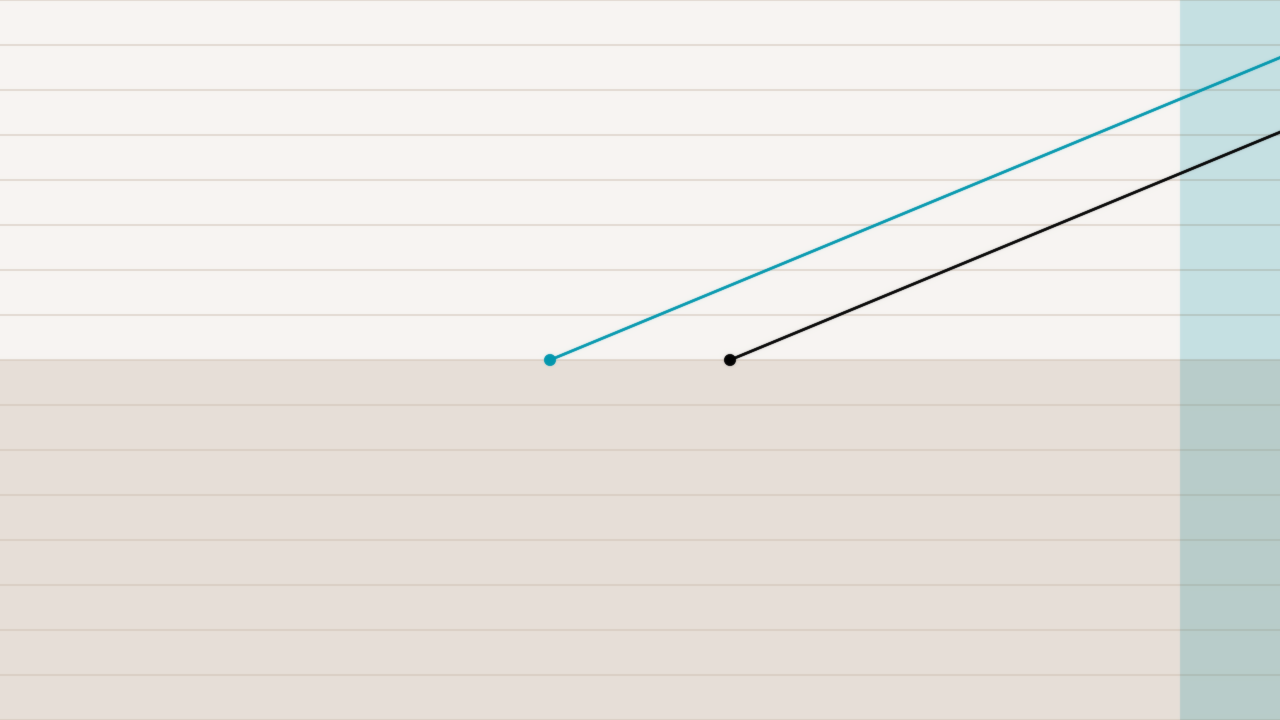
\includegraphics[width=6.5cm]{figures/rays_ge6.png}
\hspace{0.5cm}
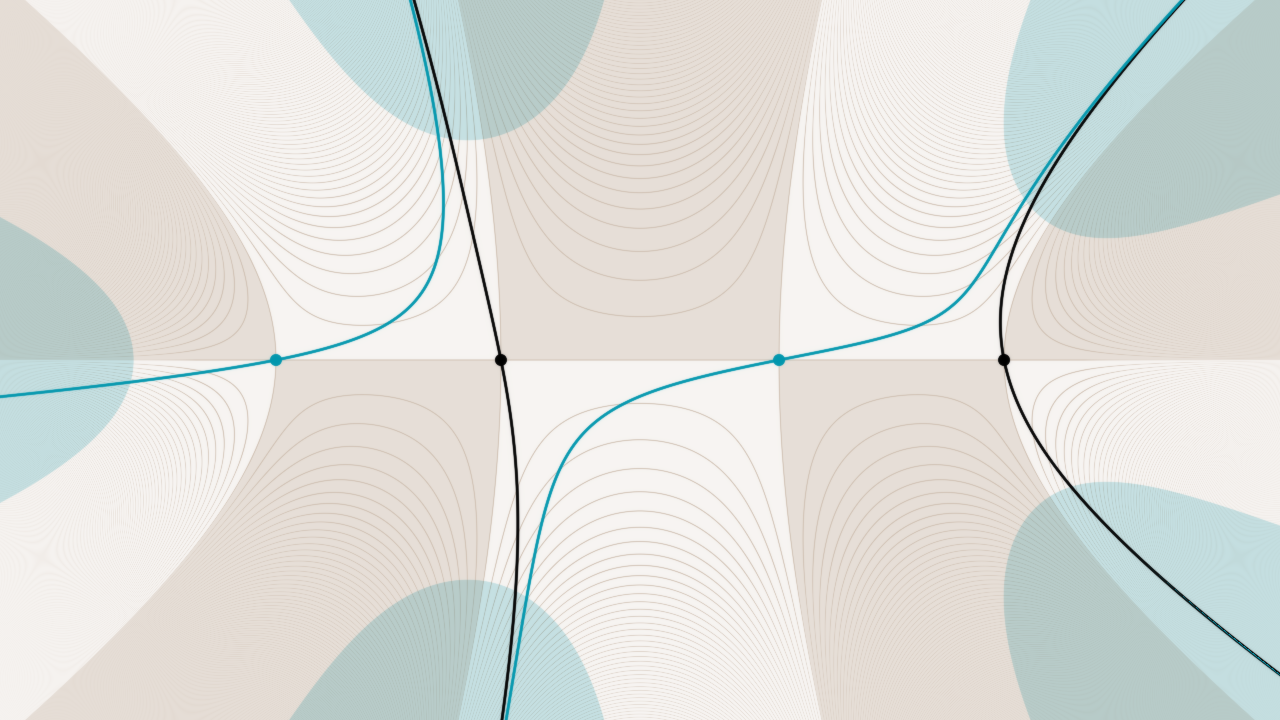
\includegraphics[width=6.5cm]{figures/thimbles-n5.png}
\captionof{figure}{The rays $\mathcal{J}^{\pi/8}_{\zeta, \pm 1}$ on the position domain, and their preimages in the $u$ plane.}\label{fig:thimble_vs_rays}
\end{center}
Choose a critcal point $a$ of $f$, noting the associated critical value $\alpha = f(a)$, and let $I_\alpha$ be a thimble integral through the thimble $\mathcal{C}_a^\theta$:
\begin{equation}
I_\alpha(z)\defeq\int_{\mathcal{C}_a^\theta}e^{-zf}\nu.
\end{equation}
Our main results show that $I_\alpha$ is Borel regular as a conseuqence of the fact that thimble integrals can be turned into a Laplace transform on the ray $f(\mathcal{C}_a^\theta)$. \textcolor{RoyalBlue}{[say more about this?]}. \textcolor{orange}{[As a start\ldots]} We recall the well-known result\color{black}
\begin{lemma}\label{lem:thimble_proj_formula}
A function $\iota$ with $I_\alpha = \laplace_{\zeta, \alpha}^\theta \iota$ is given by the {\em thimble projection formula}
\begin{equation}\label{eqn:formula}
\iota_\alpha = \frac{\partial}{\partial \zeta} \left( \int_{\mathcal{C}^\theta(\zeta)}\nu \right),
\end{equation}
where $\mathcal{C}^\theta(\zeta)$ is the part of $\mathcal{C}_a^\theta$ that goes through $f^{-1}([\alpha,\zeta e^{i\theta}])$. Notice that $\mathcal{C}(\zeta)$ starts and ends in $f^{-1}(\zeta)$. \textcolor{magenta}{[The thimble $\mathcal{C}$ needs an orientation, but the orientation is arbitrary.]}
\end{lemma}
%\begin{remark}
%The operator $\fracderiv{1/2}{\zeta}{\alpha}$ is the fractional derivative based at $\zeta = \alpha$, as defined in Section~\ref{L-int-op}:
%\begin{align*}
%\partial^{1/2}_{\zeta, \alpha} & \defeq \tfrac{\partial}{\partial \zeta} \, \partial^{3/2}_{\zeta, %\alpha} \\[2mm]
%[\partial^{3/2}_{\zeta, \alpha} g](p) & \defeq \frac{1}{\Gamma(\tfrac{1}{2})} \int_{\zeta = \alpha}^p \big(\zeta(p)-\zeta\big)^{-1/2} g\,d\zeta.
%\end{align*}
%\begin{verify}
%\begin{align*}
%[\partial^{0+1/2}_{\zeta, \alpha} f](p) & = \left(\tfrac{\partial}{\partial \zeta}\right)^{0+1} \partial^{1/2-1}_{\zeta, \alpha} \\
%& = \left(\tfrac{\partial}{\partial \zeta(p)}\right)^{0+1} \frac{1}{\Gamma(1-1/2)} \int_{\zeta = \alpha}^p \big(\zeta(p)-\zeta\big)^{-1/2} f\,d\zeta
%\end{align*}
%\end{verify}
%\end{remark}
Then, the Borel regularity of thimble integrals is established by the following theorem: 
\begin{theorem}\label{thm:maxim}
If the integral defining $I_\alpha$ is absolutely convergent, then $I_\alpha$ is Borel regular. More explicitly: \textcolor{magenta}{[change restatement to match]}
\begin{enumerate}
\item\label{part-1} The function $I_\alpha$ has an asymptotic expansion $\series{I}_\alpha \defeq \aexp^\theta I_\alpha$, which lies in the space $e^{-z \alpha} z^{-1/2} \C\llbracket z^{-1}\rrbracket$. Here, $\theta$ is the direction of the ray $\mathcal{J}^\theta_{\zeta, \alpha}$ that defines the thimble.
\item\label{part-2} The Borel transform $\tilde{\iota}_\alpha \defeq \borel_\zeta \tilde{I}_\alpha$ converges near $\zeta=\alpha$.
\item\label{part-3} The sum of $\tilde{\iota}_\alpha$ can be analytically continued along the ray $\mathcal{J}_{\zeta, \alpha}^\theta$. Its Laplace transform along that ray is well-defined, and equal to $I_\alpha$.
\end{enumerate}
\end{theorem}
%\color{Goldenrod}
%Then, our main result for thimble integrals is proving they are indeed Borel regular:
%\begin{theorem}[see Theorem \ref{thm:maxim-dim}]
 %   Let $\tilde{I}_{j}(z)\in e^{-z \alpha_j} z^{-1/2} \C\llbracket z^{-1}\rrbracket$ be the asymptotic expansion of $I_j$ as $\Re z e^{i\theta}\to \infty$ for the generic direction $\theta$. Then:
%\begin{enumerate}
%\item The series $\tilde{\Phi}_j:=z^{1/2} \tilde{I}_j$ is $1$-Gevrey, thus $\tilde{\phi}_j(\zeta)\defeq\borel_\zeta(\tilde{\Phi}_j)$ converges near $\zeta=\alpha_j$
%\item If you continue the sum of $\tilde{\phi}_j$ along the ray $ e^{i\theta}[\alpha_j,+\infty)$, and take its Laplace transform along that ray, you'll recover $z^{1/2} I_j$.
%\item\label{part3} For any $\zeta$ on the ray going rightward from $\alpha_j$, we have a \textit{thimble projection formula}
%\begin{multline}
%\hat{\phi}_{j}(\zeta)=\fracderiv{3/2}{\zeta}{\alpha_j} \left( \int_{\mathcal{C}_j(\zeta)}\nu \right)=\left(\tfrac{\partial}{\partial \zeta}\right)^2\,\frac{1}{\Gamma\big(\tfrac{1}{2}\big)} \int_{\alpha_j}^\zeta (\zeta-\zeta')^{-1/2}\left( \int_{\mathcal{C}_j(\zeta')} \nu \right)\,d\zeta',
%\end{multline}
%where $\mathcal{C}_j(\zeta)$ is the part of $\mathcal{C}_j$ that goes through $f^{-1}([\alpha_j, \zeta])$. Notice that $\mathcal{C}_j(\zeta)$ starts and ends in $f^{-1}(\zeta)$. \textcolor{magenta}{[The thimble $\mathcal{C}_j$ needs an orientation, but the orientation is arbitrary.]}
%\end{enumerate}
%\end{theorem}
%\color{black}
\color{RoyalBlue}
\textcolor{orange}{[Shorten, but maybe keep the basics.]} We sketch the proofs of the main results in the following diagram (for the rigorous ones see Section~\ref{borel-reg-thimble}):
%\[
%\begin{tikzcd}
%{I} \arrow[rrr,"\aexp^{\theta}"]\arrow[dd, swap,"\laplace^{-1} "] &  & & \tilde{I}\arrow[dd,"\borel"]\\
%& & &\\
%\iota \arrow[r,equal] & \hat{\iota} & &\tilde{\iota} \arrow[ll, "\text{sum}"]
%\end{tikzcd}
%\]
On the one hand, with a change of coordinates, the thimble integral $I$ can be written as a Laplace type integral, i.e. as the Laplace transform of a function $\iota$, written explicitly in equation~\eqref{eqn:formula}. 
On the other hand, we compute the asymptotic expansion of $I$ using the saddle point approximation, which turns out to be a formal $1$-Gevrey series in the frequency domain. Consequently, its Borel transform $\series{\iota}$ is a germ of holomorphic functions at $\zeta=\alpha$ in the position domain. Finally, we will show that the Taylor expansion of $\iota$ at $\zeta=\alpha$ agrees with~$\tilde{\iota}$.

\textcolor{magenta}{Discuss where to find proofs, similarly to \texttt{reg-sing-volterra}.}
\color{black}
%% the following remark has been moved to Section of the proof
%\begin{remark}\label{rmk:Pham formula}
%    Equation \eqref{eqn:formula} gives an explicit expression for $\phi_j$ in terms of $\nu$ and of the pre-image of the ray $e^{i\theta}[\alpha_j,\zeta)$ via $f$. When $f$ and $\nu$ are polynomials and $X$ is $N$-dimensional, a result of Pham \cite[Equation 2.4, II partie]{pham} allows to write $\hat{\iota}_j$ explicitly as 
%    \begin{equation}\label{eqn:Pham}
 %       (-1)^{\frac{N(N-1)}{2}}  \sum_{k=0}^\infty c_k\, \delta^{-\frac{N}{2}-k}+ \text{ hol. funct.}
 %   \end{equation}
%for some coefficients $c_k$ which depends on $f$ and $\nu$, and with $\delta^{-\alpha}$ be defined as
 %  \begin{equation*}
  %     \delta^{-\alpha}:=\begin{cases}
   %        \frac{\zeta^{\alpha-1}}{-2\pi i(\alpha-1)!}\log(\zeta) + \text{ hol. funct.} & \text{ if } \alpha\in\mathbb{N}^*\\
    %       & \\
     %      \frac{(-\zeta)^{\alpha-1}}{2\pi i \Gamma(-\alpha)}+ \text{ hol. funct.} & \text{ if } \alpha\notin \mathbb{N}^* 
      % \end{cases}
   %\end{equation*}
%In particular, if $N=1$, from equation \eqref{eqn:Pham} we deduce that $\hat{\phi}_j$ is the $1/2-$ derivative of $\hat{\iota}_j$, \textcolor{orange}{hence it has simple singularities \ref{simple-res-thimble}.} We expect this result to hold beyond the polynomial case. We also expect that equation \eqref{eqn:formula} can be generalized to the $N$-dimensional case replacing the $3/2$-derivative with the $(N+1)/2$ one. 
%\end{remark}
%     
\subsubsection{Other results}
%
In our study of Borel regularity, we use some new perspectives on the Laplace transform, discussed in Section~\ref{sec:Laplace-Borel-general}.

Laplace transform methods for solving ODEs on the frequency domain traditionally relate them to ODEs on the position domain. We find, however, that it is easier and more natural to relate ODEs on the frequency domain to integral equations on the position domain. In particular, the good behavior of integral equations and their solutions is central to our proof that certain ODEs have Borel regular solutions.

In Sections \ref{sec:geometry_laplace} and \ref{sec:geometry_borel}, we introduce a geometric picture of the Laplace and Borel transforms, generalizing the position domain from the complex plane to a translation surface $B$. Each translation chart $\zeta$ gives a different version of the Laplace transform, whose associated frequency domain is the cotangent space $T^*_{\zeta = 0} B$. The frequency coordinate $z$ is a canonical coordinate on $T^*_{\zeta = 0}B$, or on $T^*_{\zeta = 0}B^{\otimes n}$ if $\zeta = 0$ is a singularity with cone angle $2\pi n$.
\begin{center}
\phaseSpaceLaplace
\captionof{figure}{The frequency coordinate $z$ on the cotangent spaces of an ordinary point and a singular point. The singularity shown here has cone angle $6\pi$, like the singularities of the translation surface associated with the Airy function.}
\end{center}

We illustrate our main results with detailed treatments of several examples: we will mostly focus on degree two ODEs that admit a frame of solutions expressed as thimble integrals: the Airy--Lucas functions (Section~\ref{example_AL}), the modified Bessel functions, the Airy function (Appendix~\ref{airy-appendix}), \textcolor{red}{the anharmonic oscillator...).} On the one hand, we explicitly solve the integral equation associated with the ODE, building a frame of analytic solutions which are Laplace transforms. On the other hand, our \textit{thimble projection reasoning} shows how to rewrite explicitly thimble integrals as a Laplace transform and it makes Borel regularity evident directly from explicit computations. The thimble projection reasoning is the one we use in Lemma~\ref{lem:thimble_proj_formula} and it is crucial for the proof of Theorem~\ref{thm:maxim}. In the Airy example (see Section~\ref{airy-appendix}) we will compute the \textit{thimble projection formula} directly.%, and by numerical check we show $\hat{\phi}\defeq\fracderiv{-1/2}{\zeta}{\alpha}\iota$ is a simple resurgent function (see Section~\ref{apx:eye-res-airy}).

Among the examples we study, some of them have been discussed many times, using different approaches and conventions. We try to give an idea of how all these different treatments fit together. For instance, for the Airy function we will make a comparison with \cite[Section 2.2]{lectures-Marino}, \cite[Section 6.14]{diverg-resurg-i}, and \cite[Section 2.2]{kawai-takei}. \textcolor{red}{The anharmonic oscillator was also discussed in (\cite{bender-wu}, \cite[Appendix B]{aniceto2019primer} and \cite[Section 2.5.3]{sternin1995borel}).} Other examples haven't been discussed much, as for Airy--Lucas functions \cite[Equation 3.2]{charbonnier22}.

Recently, resurgence theory (first developed by \'Ecalle in the '80) has attracted interest in mathematics and physics. The resurgence of linear ODEs have been intensively studied \cite{loday1994stokes,diverg-resurg--ii} and many results are also known for non-linear ODEs \cite{costin-PI,costin_kruskal,diverg-resurg-iii,schiappa-PI}. For algebraic thimble integrals of the type we studied in this paper, the resurgence of their asymptotic expansion can be understood geometrically (see \cite{Maxim_slide_ERC}, \cite[Section 6.2]{kontsevich2022analyticity}), however for more general exponential integrals (see the last example in \cite{Maxim_slide_ERC}) resurgence remains conjectural. Despite their simplicity, our examples of linear ODEs and of 1-dimensional thimble integrals are toy-models that show some features of resurgent functions. 

%\color{gray}
%\begin{itemize}
%\item The central goal of this paper is to lay out two kinds of problems where we can prove that the Borel sum of a formal power series solution is always an actual solution.
%\begin{itemize}
%\item The first problem is evaluating a certain kind of exponential integral: a one-dimensional {\em thimble integral}.
%\item The second problem is solving a certain kind of ODE.
%\item These two problems are closely linked. By playing with derivatives of an exponential integral, you can often find a linear ODE that the integral satisfies. Conversely, for many classical ODEs, there are useful bases of exponential integral solutions.
%\item \textcolor{magenta}{(Does this touch the Picard-Lefshetz perspective? Betti / de Rham relationship: ODE is a connection, and exponential integrals give flat sections?)}
%\end{itemize}
%
%\item Clearly separate the parts of the theory that deal with holomorphic functions and formal power series.
%\begin{itemize}
%\item we can do that also for thimble integrals (this is part 4 of Thm 5.1 in {\tt draft2.pdf})
%\end{itemize}
%\item (Super-motivation: why do the zeroes of $\lambda$ play a special role?) As part of the treatment, we've made use of some new perspectives on the Laplace transform.
%\begin{itemize}
%\item \textbf{Geometric picture.} The spatial domain $B$ is a translation surface. If $b \in B$ is non-singular, the frequency domain for $\laplace_b^\theta$ is $T^* B_b$. If $b$ is a conical singularity, the frequency domain is more interesting, as we will see in our main example.
%\item \textbf{A new dictionary for ODEs.} The Laplace transform is often used to solve ODEs on the frequency domain by relating them to ODEs on the spatial domain. We find, however, that it is much easier and more natural to relate ODEs on the frequency domain to integral equations on the spatial domain. 
%\begin{itemize}
%\item This clarifies why we take the Borel sums at zeroes of $\lambda$ when we are trying to solve an ODE.
%\end{itemize}
%\end{itemize}
%\item Our picture helps explain why it is useful to work on the Borel plane (the position domain).
%\begin{itemize}
%\item Integral equations are more regular than differential equations.
%\item A thimble integral in the frequency domain can be recast as the Laplace transform of a function in the position domain.
%\end{itemize}
%\item Illustrate with detailed treatments of several examples.
%\begin{itemize}
%\item Contour argument (thimble integrals)
%\item solving integral equation (ODE)
%\item How thimble integrals and ODE are related in our examples?
%\end{itemize}
%\begin{itemize}
%\item Some have been discussed many times, using different approaches and conventions. We will try to give an idea of how all these different treatments fit together. $\bullet$ The Airy function (Marino, Sauzin). $\bullet$ The anharmonic oscillator (Bender--Wu, Schiappa).
%\item Others haven't been discussed much.
%\end{itemize}
%\item Recently, resurgence theory (first developed by \'Ecalle in the '80) has attracted interests in math and physics as a powerful alternative to Borel summability. Resurgence of lienar ODEs have been studied (see Costin slides for ReNewQuantum). Many results are also known for non linear ODEs (see Schiappa PI, Costin PI). For algebraic exponential integrals of the type we studied in this paper, resurgence of their asymptotic expansion can be understood geometrically (see Maxim's slides ReNewQuantum), however for more general exponential integrals (see examples in Maxim's talk) resurgence remains a conjecture. Despite their simplicity, our examples of linear ODEs and of exponential integrals show some features of resurgence and they are toy model to get a feeling on \'Ecalle formalism.       
%\item \textcolor{magenta}{The examples give a place to compare more complicated formalisms like the Picard-Lefshetz (Morse theory) or Ecalle formalisms? [How do we work this into the introduction?]}
%\begin{itemize}
%\item thimble integrals are geometric in the sense of being pairing between homology and cohomology 
%\item computation of Stokes constants via Picard--Lefschetz theory
%\end{itemize}
%\end{itemize}

%\subsection{Why does Borel resummation work?}
%
%\color{gray}
%
%Borel resummation is a way of turning a formal power series
%\[ \series{\varphi} = z^\sigma \left( \frac{\varphi_0}{z} + \frac{\varphi_1}{z^2} + \frac{\varphi_2}{z^3} + \frac{\varphi_3}{z^4} + \ldots \right), \]
%with $\sigma \in [0, 1)$, into a function which is asymptotic to $\series{\varphi}$ as $z \to \infty$. Different functions can be asymptotic to the same power series, and Borel resummation picks one of them, performing an implicit regularization~\textbf{[arXiv:1705.03071, or maybe arXiv:1412.6614]}. When a function matches the Borel sum of its asymptotic series, we will say it is {\em Borel regular}. Several familiar kinds of regularity imply Borel regularity, and shed light on why it occurs.
%%%Knowing that a function is Borel regular gives us extra information about it---enough to reconstruct it from its asymptotic series. What's the nature of this extra information?
%%%Since different functions can be asymptotic to the same power series, Borel resummation must involve an {\em implicit regularization}, restricting its range to a class of functions which are uniquely determined by their formal power series.
%\begin{itemize}
%\item \textbf{Having a good asymptotic approximation}
%
%Let $R_N$ be the difference between a function and the partial sum
%\[ \frac{\varphi_0}{z} + \frac{\varphi_1}{z^2} + \frac{\varphi_2}{z^3} + \ldots + \frac{\varphi_{N-2}}{z^{N-1}} \]
%of its asymptotic series. Watson showed a century ago that the function is Borel regular whenever there is a constant $c \in (0, \infty)$ with
%\[ |R_N| \le \frac{c^{N+1} N!}{|z|^N} \]
%over all orders $N$ and all $z$ in a wide enough wedge around infinity (Sokal, ``An improvement of Watson's theorem on Borel summability''; Hardy, {\em Divergent Series}, Theorem~136; Watson, ``A theory of asymptotic series,'' \S 8?).
%\color{black}
%
%\item \textbf{Satisfying a singular differential equation}
%
%\begin{itemize}
%\item This is the setup. We restrict to ODEs with irregular singularity at $\infty$ and of Poincaré rank $1$: 
%\begin{equation}\label{eqn:standard ODE}
%\Big[ P(\partial_z)+\frac{1}{z}Q_1(\partial_z)+\sum_{j=2}^d z^{-j}R_j(\partial_z)\Big]\Psi=0
%\end{equation}
%where $P(\lambda)$ is a (monic) degree $d$ polynomial, $Q(\lambda)$ is a degree $d-1$ polynomial and $R_j$ is a degree $d-j$ polynomial. \textcolor{magenta}{[Looking at the existence theorem in {\tt airy-resurgence} 2.1.3, we could apply this reasoning on the analytic side for more general equations, but this particular case makes it easier to talk about the formal side as well.]} Furthermore we assume $P$ has simple zeros $P(\alpha_j)=0$, $j=1,...,d$ and $Q(\alpha_j)\neq 0$.
%\item \color{DarkTurquoise}
%I think we can go more general? If I'm not mistaken, \'{E}calle's equation form \cite[equation~2.2.3, p.~105]{EcalleIII} covers operators like
%\[ P(\partial_z) + \frac{1}{z} Q_1(\partial_z) + \frac{1}{z^2}\big[ R_0(z^{-1}) + R_1(z^{-1})\,\partial_z + \ldots + R_d(z^{-1})\,\partial_z^d \b], \]
%where $P$ and $Q$ are as above, and $R_0, \ldots, R_d$ are holomorphic functions on $\C$.
%\color{black}
%\item (backgrounds) Under these assumptions, 
%\begin{itemize}
%\item \eqref{eqn:standard ODE} admits a basis of formal solutions: let $\tau_j:=Q(-\alpha_j)/P'(-\alpha_j)\in\mathbb{Q}^*$, then the formal solutions $\tilde{\Psi}_1,...,\tilde{\Psi}_d$ are of the form \cite{int-irreg} \cite[Proposition~2.2.7, p.~111]{EcalleIII}
%\begin{equation}
%\label{formal solution}
%\tilde{\Psi}_j(z)=e^{-\alpha_j z}z^{-\tau_j}\tilde{F}_j(z)\in e^{-\alpha_j z } z^{-\tau_j}\,\C \llbracket z^{-\tau_j} \rrbracket
%\end{equation}
%Notice that this basis is distinguished only up to scaling, so we have a distinguished frame in the space of formal solutions. 
%\item \eqref{formal solution} is Borel-Laplace summable and its Borel-Laplace sum $\Psi_j$ satisfies the original equation \eqref{eqn:standard ODE}
%\item as a consequence, the distinguished frame of formal solutions become a distinguished frame of analytic solutions $\Psi_1,...,\Psi_d$.  
%\end{itemize}
%\item Can we see there exists a distinguished basis in a purely analytic way? YES. [Thm 1]% The reason is the existence theorem gives for every $\alpha_j$ a unique solution in the $\zeta$-plane which blows-up in a certain way at $\alpha_j$: ${\phi}_j(\zeta_j)=\zeta_j^{-\tau_j}+\tilde{f}_j$, $\zeta_j=\zeta-\alpha_j$.
%\item why Borel summations of $\tilde{\Psi_1},...,\tilde{\Psi_d}$ finds this solutions? because they are an analytic frame of Borel regular functions. 
%\begin{itemize}
%\item {[Thm 1]}: for every $\alpha_j$ there exists a unique solution in the $\zeta$-plane which blows-up in a certain way at $\alpha_j$: ${\phi}_j(\zeta_j)=\zeta_j^{-\tau_j}+\tilde{f}_j$, $\zeta_j=\zeta-\alpha_j$. (proof based on existence theorem \ref{frac_int_exist})
%\item {[Thm 2]}: The Borel sum of the formal solutions $\tilde{\Psi}_j$ are the same as the Laplace transform of the solutions of Thm 1. 
%\item Cor of Thm 2: the Laplace transform of solutions of Thm 1 are Borel regular.   
%\end{itemize}
%\item Say there is a unique solution (up to scaling) that shrinks as you go right; everything else blows up exponentially. Then this is the only solution that can be expressed as a Laplace transform. [Follows from Aaron's argument in Airy resurgence, even if Aaron works with more general ODEs]
%
%\item Draw diagram showing formal vs. holomorphic solutions in time vs. frequency domains.
%
%\begin{center}
%\begin{tikzcd}
%& & ODE\arrow[dd,"\borel"]\arrow[dd,"\laplace^{-1}",swap] & & \\
%\Phi\arrow[rru,dotted, no head, tail] &\textcolor{red}{\hat{\Phi}}\arrow[ur,red, no head, tail] & & & \tilde{\Phi}\arrow[llu,"formal",swap, no head, tail]\arrow[dd,"\borel"]\\
%& & IE & & \\
%\phi\arrow[rru, no head, tail]\arrow[uu,"\laplace"]& \textcolor{red}{\hat{\phi}}\arrow[ur, no head, tail]\arrow[rrr,"sum",mapsfrom,red]\arrow[uu,"\laplace"]& & & \tilde{\phi}\arrow[llu, no head, tail]
%\end{tikzcd}
%\end{center}
%
%where the arrow in red are a consequence of multisummability. In addition, we can distinguish on the right hand side of the diagram the formal solutions and on the left hand side the holomorphic ones. On the upper part of the diagram the functions in the $z$-plane while on the lower part the functions in the Borel plane $\zeta$-plane.
%\item  
%there are many ways to see this problem have a distinguished base of solutions, Poincar\'e see it formally in the $z$-plane, \textcolor{red}{\'Ecalle figured it out how to see it formally in the Borel plane}, our results shows how to see it analytically in  the Borel plane.
%\item  M.A.E.T. says you can start in formal $z$-plane but it is not really constructive (see Balser chap 14); going from formal $\zeta$ to analytic is constructive and it is essentially Borel-Laplace summation. Our method uses just Laplace transform. 
%\item How do we know we are picking the same frame? from properties of Laplace transform we get solution asymptotics to Poincar\'e frame. From uniqueness result we get a frame equivalent to \'Ecalle's frame. 
%\item multi-summability is a regularity result starting form the formal solution in the $z$-plane. Borel regularity is instead based on the analytic solution in the $z$-plane. The argument we gave about getting the same frame is what proves Borel regularity of $\Psi_j$.   
%\end{itemize}
%
%\color{DarkBlue}
%
%\item \textbf{Being a thimble integral}
%
%\begin{itemize}
%\item This is the setup. Let $X$ be an algebraic variety of dimension $N$, $f\colon X\to \mathbb{C}$ be a holomorphic Morse function with only simple critical points and $\nu\in\Gamma(X,\Omega^N)$.
%\begin{itemize}
%\item recall theory of homology and cohomology to define the thimbles integrals. Pham has briefly discussed it, but apparently was introduced by Malgrange, Milnor and ?.  
%\end{itemize} 
%\item background: Pham prove Borel regularity for exponential integral in N-dimension and without assuming Morse critical points (but only isolated). His proof is geometric [it may be useful to add it in Appendix]. 
%\item \textcolor{red}{We give an analytic proof analogous of Pham.}
%\item I think we should separate what can we do in general for N-dimensional integral and what is special for the $1$-dimensional one. 
%\item {[Thm 4]} 1-dim thimbles integrals are Borel regular, namely let 
%\begin{equation}
%I_{\alpha}(z)\defeq\int_{\mathcal{C}_\alpha}e^{-zf}\nu
%\end{equation}
%
%then the following diagram is commutative
%\begin{equation}
%\begin{tikzcd}
%I_{\alpha}(z) \arrow[r,"\ae^\theta"] & \tilde{I}_{\alpha}(z)\arrow[dd,"\borel"]\\
%& \\
%\hat{\iota}_\alpha(\zeta)\arrow[uu, "\laplace^\theta_\alpha "] & \tilde{\iota}_{\alpha}(\zeta) \arrow[l, "\text{sum}"]
%\end{tikzcd}
%\end{equation}
%\begin{itemize}
%\item on the one hand take asymptotic expansion of integral via saddle point approximation and then study the Borel Laplace sum of the divergent series [from left upper corners clockwise]
%\item on the other hand \textcolor{red}{see that the thimble integral is a generalized Laplace transform (which in certain cases can be rewritten as a usual Laplace transform).}
%\item A priori, the Laplace transform of $\hat{\iota}_\alpha(\zeta)$ and $I_{\alpha}(z)$ have the same asymptotic behaviour in a given sector (indeed taking the asymptotic of $I_\alpha(z)$ we \textit{loose} information); however Borel regularity guarantees that $I_{\alpha}(z)=\laplace^{\theta}\hat{\iota}_{\alpha}$ in a given sector.
%\item A corollary of [Thm 4] is the fractional derivative formula.
%\item Conjecturally, we expect $\hat{\varphi}_\alpha(\zeta)$ to have simple singularities. 
%\end{itemize}
%\item From the result of Pham we can deduce Stokes constants are always integers as they are intersection numbers (use same argument of Maxim). See also the argument of KS21 sec 6.2 in the framework of analytic WCFs. Prove integrality of Stokes constants using the fractional integral formula vs differential equation (see example in Appendix C) 
%\end{itemize}



%\subsection{Stokes phenomenon}
%\begin{itemize}
%\item For Bessel functions, we can see explicitly how solutions jump when the Laplace transform angle crosses a critical value.
%\item The jump comes from the branch cut difference identity for hypergeometric functions.
%\item Possible interpretation of the Stokes factors as intersections numbers in Morse--Novikov theory \textbf{[ask Maxim]}
%\end{itemize}
\subsection{Plan of the paper}
The paper is organized as follows: in Section~\ref{sec:historical-context} we review some well-known results concerning Borel regularity which dates back to the classical theory of asymptotics, ODEs and integrals over Lefschetz thimbles. This could help the reader to contextualize our results in the literature. Then, in Section~\ref{sec:Laplace-Borel-general} is devoted to define the new geometric picture of the Borel and Laplace transform. The reader who is not familiar with the formalism of Borel and Laplace transforms might start with Sections \ref{laplace:ordinary}, the beginning of Section~\ref{sec:geometry_borel} and of Section~\ref{sec:borel-laplace-homom}. Then, Section~\ref{sec:proof_main_results} contains proofs of the main results. Finally, in Section~\ref{sec:examples} we give a detailed treatment of different examples both from the ODE perspective and from the thimble integral one. 
We include Appendix~\ref{airy-appendix} that contains a detailed treatment of the Airy example, and it is recommended for readers less familiar to the subject. \textcolor{red}{The second one, Appendix~\ref{apx:generalities_ODEs}, reviews the main aspects of \cite{reg-sing-volterra}.}  
%
\subsection{Acknowledgements}
This paper is a result of the ERC-SyG project, Recursive and Exact New Quantum Theory (ReNewQuantum) which received funding from the European Research Council (ERC) under the European Union's Horizon 2020 research and innovation programme under grant agreement No 810573. 

We thank Fondation Mathematique Jacques Hadamard for supporting the visit of the second author at IH\'ES, under the program \textit{Junior Scientific Visibility}. 

We thank Maxim Kontsevich, David Sauzin, Fr\'ed\'eric Fauvet, Andrew Neitzke, for fruitful discussions and suggestions. 
%
\section{Historical context}\label{sec:historical-context}
%
\subsection{Borel regularity as a good approximation condition}
Borel regular functions can be characterized as functions that are approximated well, asymptotically, by polynomials. Watson showed a century ago \cite[Part II, Section 9]{watson2} that a function $\Phi$ is Borel regular whenever its asymptotic expansion for large $|z|$ is uniformly $1$-Gevrey-asymptotic in an obtuse-angled sector at infinity (see Definition~\ref{def:unif-gevrey-asymp}).

Watson's theorem was soon improved by Nevanlinna \cite{nevanlinna} (see a modern proof in \cite[Theorem~B.15]{nikolaev2023exact} and a generalization to power series with fractional power exponents in \cite{delabaere--rosoamanana}), and improved again later by Sokal \cite{sokal1980improvement}. These improvements tell us that the obtuse-angled sector around $\infty$ in the statement above can be replaced with an open disk whose boundary touches infinity---that is, an half-plane which does not contain $0$, and may be displaced from $0$ by some distance $\Lambda$.
\begin{center}
\begin{tikzpicture}
\setfiberscale{2.5}
\renewcommand{\phase}{35}
\newcommand{\dis}{1.2}
\begin{fiber}[shade, phase=\phase, dis=\dis]
\genfibercontent[dual]
\draw (0, 0) -- (-\phase:\rshade);
\draw[rotate=-\phase] (\dis, -0.1) -- (\dis, 0.1);
\draw (0, 0) -- (0.75, 0);
\draw[shorten <=0.3mm, shorten >=0.3mm] (0:0.5) arc (0:-\phase:0.5) node[midway, anchor=180-\phase/2] {$-\theta$};
\node[anchor=90-\phase, inner sep=2mm] at (-\phase:\dis) {$\Lambda$};
\node[anchor=north west, inner sep=2mm] at (-\rfiber, \rfiber) {$z$};
\end{fiber}
\end{tikzpicture}
\end{center}
When the half-plane extends along the $-\theta$ direction, the sum $\hat{\phi}$ of the Borel transform of $\aexp^{-\theta} \Phi$ has an absolutely convergent Laplace transform along the $\theta$ direction. In fact, we have $|\hat{\phi}| \lesssim e^{\Lambda |\zeta|}$ uniformly over a constant-radius neighborhood of the ray $\zeta \in e^{i\theta}[0, \infty)$. 
\begin{center}
\begin{tikzpicture}
\setfiberscale{2.5}
\pgfmathsetmacro{\rshade}{1.5*\rfiber}
\renewcommand{\phase}{35}
\newcommand{\radius}{0.85}
\begin{fiber}
\fill[pwbeige!30, rotate=\phase] (\rshade, \radius) -- (0, \radius) arc (90:270:\radius) -- (0, -\radius) -- (\rshade, -\radius) -- cycle;
\genfibercontent
\draw (0, 0) -- (0.75, 0);
\draw[ray] (0, 0) -- (\phase:\rshade);
\draw[shorten <=0.3mm, shorten >=0.3mm] (0:0.5) arc (0:\phase:0.5) node[midway, anchor=180+\phase/2] {$\theta$};
\node[anchor=north west, inner sep=2mm] at (-\rfiber, \rfiber) {$\zeta$};
\end{fiber}
\end{tikzpicture}
\end{center}

The Watson--Nevanlinna--Sokal characterization of Borel regular functions is totally general, which means it cannot  take advantage of any extra structure provided by the problem you are trying to solve. We take the opposite approach, showing that certain functions are Borel regular just because of the extra structure provided by the problems they solve. 

%%a function $\Phi$ holomorphic in a sectorial neighbourhood $\mathsf{A}_\theta:=\{z\in\C \vert \Re(e^{i\theta}z)\}$ is Borel regular. Indeed let $\series{\Phi}\in\C\llbracket z^{-1}\rrbracket$ be the ``Gevrey-asymptotics'' of $\Phi$ as $\Re(e^{i\theta}z)\to \infty$, then its Borel transform $\hat{\phi}\defeq\borel\series{\Phi}$ is a germ of holomorphic function at the origin and it can be analytically continued in a tubular neighbourhood of the ray $e^{i\theta}[0,\infty)$ with at most exponential growth at infinity. Hence $\Phi$ is Borel-regularizable. In addition, $\series{\phi}$ converges uniformly to a holomorphic function $\phi(\zeta)$ whose Laplace transform coincides with $\Phi(z)$. In particular, we learn that being ``Gevrey-asymptotic'' to a formal series is a sufficient condition for Borel regularity. 
\subsection{Borel regularity for level~$1$ ODEs}
%
The study of irregular singular differential equations in the complex domain has a long history, and interesting phenoma distinguish irregular singular equations to regular singular ones. Already at the formal level, irregular singular ODEs have a distinguished behaviour, namely they admit divergent formal series solutions in the form of trans-monomials. In particular, for level $1$ ODEs of the kind we study in this paper, the Poincar\'e method gives an algorithm to compute formal solutions of $\mathcal{P}\Phi=0$, see~\cite{int-irreg}\cite[Proposition~2.2.7, p.~111]{EcalleIII}. Then, the main question is how to ``promote'' a formal solution to an analytic one, and here is where summability methods will play a r\^ole~\cite{loday-Remy2011,diverg-resurg--ii,malgrange--fourier,malgrange1995sommation,malgrange92,ramis1991series}. In fact, even if it is not contructive, the Main Asymptotic Existence Theorem (M.A.E.T.) guarantees the existence of an analytic frame of solutions asymptotic to the formal one (see~\cite[Chapter 14]{balser}). Then, the Ramis Index Theorem shows that the formal solutions $\tilde{\Phi}$ of $\mathcal{P}\Phi=0$ are 1-Gevrey series---the first step in proving Borel~summability~\cite{ramis_index}.  \textcolor{orange}{[Mention connection to index, in Loday-Richaud, and to the way orders get shifted?]} Furthermore, after checking the solution $\series{\Phi}$ is Borel summable, another argument is needed to show that the Borel sum solve the original equation---a priori, the Borel sum is only Gevrey asymptotic to the solution $\series{\Phi}$. 

Still based on Borel summation, the approach of resurgence introduced by \'Ecalle in the '80 emphasizes the r\^ole of the position domain. Indeed, differential equation in the frequency domain can be turned into integral equation in the position domain, using the Borel transform. In particular the Borel transform of the formal solution $\series{\Phi}$ is a germ of analytic functions, and its analytic properties can be studied in terms of the equation they satisfy. For instance, in~\cite{loday-Remy2011}, Loday-Richaud and Remy solve perturbed integral equations formally in the position domain (following the approach of \'Ecalle~\cite{EcalleIII}). Yet working in the position domain, one can turn the integral equation into a differential equation and trying to solve it analytically in the position domain, see~\cite{malgrange--fourier}. Then, going back to the frequency plane can be done with the Laplace transform, but it is usually a technincal analytic step. However, the advantage of resurgence compared to the usual Borel summation, is in the study of the Stokes phenomena, which is another distinguished feature of irregular singular ODEs. Indeed, the Stokes phenoma is closely related to the fact that formal solutions are divergent, and the so called Stokes constants encode the ``jumps" of the underlying analytic solution which is deifned on sectors of openening angle $\pi$ and when extended by continuation on larger sectors it jumps by an exponentially small correction. As an example, the first order equation \[\Phi'=\Phi+\frac{1}{z}\] has formal solution $\series{\Phi}=\sum_{n=0}^\infty n!z^{-n-1}$. Then, its Borel transform has a simple pole at $\zeta=1$. Consequently, the ``jump'' of its Borel sum occurs across the positive real axis $\Re(z)>0$ and it is given by $2\pi ie^{-z}$. 

In a nutshell, the aim of resurgence is to study the analytic continuation of the Borel transform of a divergent series, in particular the location of sngularities in the position domain and Stokes constants computed after analytic continuation across the singularities. Then, the set of Stokes data (namely the Stokes ray emanating from the singulairties and the associated Stokes constants) give the input to set-up a Riemann--Hilbert problem, whose solution would be a frame of analytic solutions of the ODEs~\cite{kontsevich2022analyticity}.

So far we have been discussed the classical approaches to summability and reusrgence of formal solutions of irregular singular ODEs, but a different approach would be to look for analytic solutions of $\mathcal{P}\Phi=0$. In other words, we can solve irregular singular ODEs in the frequency domain starting with an analytic \emph{ansatz}. Here the standard approach is the so called Laplace method, which takes as \emph{ansatz} a Laplace transform integral. This is the approahc we adopt in this paper, but our choice of Laplace transform integral to begin with is very special, i.e. it is a Borel regular solution. As for \'Ecalle's method, the Laplace transform method turns differential equations in the frequency domain into integral equations in the position domain. Indeed, building on our results of~\cite{reg-sing-volterra}, our approch will take the advantage of working on the position domain. A similar approach was taken by Braaksma in~\cite{braaksma2006laplace}, where also the same function spaces we will introduce in Section~\ref{sec:laplace_analytic} have been used to solve system of ODEs whose coefficients are in the form of Laplace transforms. However, with our approach, we can solve differetial equations with more general coefficients, and we plan to extend our results to systems of ODEs and generalize Braaksma's results. 

Summarizing, we collect the main methods to solve irregular singular ODEs in the following table stressing the difference between formal and analytic solutions in either the frequency and the position domain.
\begin{center}
\begin{tabular}{l|l|l}
& \textbf{Analytic} & \textbf{Formal} \\ \hline
\textbf{Frequency} &  & Poincar\'{e}: trans-monomial ansatz~\cite{int-irreg} \\ \hline
\textbf{Position} & \'{E}calle: resurgence  & \'{E}calle: formal perturbation theory~\cite{EcalleIII,loday-Remy2011} \\
& Fixed-point iteration~\cite{reg-sing-volterra} \\
\end{tabular}
\end{center}


\color{RoyalBlue}
From a formal perspective, the general theory of linear level~$1$ ODEs suggests to look for formal solutions $\tilde{\Psi}_\alpha$ of $\mathcal{P}\Phi=0$ in the transmonomial space $\tilde{\Psi}_\alpha\in e^{-\alpha z} z^{-\tau_\alpha}\C\llbracket z^{-1}\rrbracket$, where $\tau_\alpha=Q(-\alpha)/P’(-\alpha)$~\cite{int-irreg}\cite[Proposition~2.2.7, p.~111]{EcalleIII}. Since the cirtical values are distinct, the transmonomials $\tilde{\Psi}_\alpha$ determine a basis up to scaling, giving the space of formal solutions a distinguished frame. Then, the Main Asymptotic Existence Theorem (M.A.E.T.) guarantees the existence of an analytic frame of solutions asymptotic to the formal one, but it  does not give a way to construct that analytic frame (see~\cite[Chapter 14]{balser}). To get a constructive proof, a classical approach was to investigate Borel summability of the formal solutions~\cite{loday-Remy2011,diverg-resurg--ii,malgrange--fourier,malgrange1995sommation,malgrange92,ramis1991series}. For example, the Ramis Index Theorem shows that the $\tilde{\Psi}_\alpha$ are 1-Gevrey series---the first step in proving Borel~summability~\cite{ramis_index}. \textcolor{orange}{[Mention connection to index, in Loday-Richaud, and to the way orders get shifted?]}

At the same time, a natural question we can ask is whether we can build an analytic frame of solutions, without looking for a formal frame. This is possible, as we proved in Theorem~\ref{thm:exist_uniq_ODE} (building on our previous results in~\cite{reg-sing-volterra}), and these solutions turn out to be asymptotic to the formal solutions $\tilde{\Psi}_\alpha$ (see Theorem~\ref{thm:soln_is_asymptotic}). Recall that the key aspect in the proof of our result~\cite[Theorem~4]{reg-sing-volterra} is going to the position domain and study solutions of an integral equation with a special behaviour at the singular points $\zeta=\alpha$. Although our approach and the classical one of Borel summability both focus on the importance of the position domain, we study different equations: on the one hand, we solve integral equations in the position domain; on the other hand, Malgrange solves differential equations analytically in the position domain~\cite{malgrange--fourier}, and in~\cite{loday-Remy2011}, Loday-Richaud and Remy solve perturbed integral equations formally in the position domain (following the approach of \'Ecalle~\cite{EcalleIII}). 

\begin{remark}
Our approach of solving regular singular Volterra equation---based on the contraction mapping theorem for suitable Banach spaces \cite{reg-sing-volterra}---is analogous to the one that Braaksma used to solve a different class of non-linear ODEs and difference equations whose coefficients are written as Laplace transforms~\cite{braaksma2006laplace}. \textcolor{orange}{Our approach differs from Braaksma's in two ways. [\ldots]} \textcolor{RoyalBlue}{What distinguishs our result from Braaksma's is considering the Laplace transform of functions with integrable fractional power singuarities, and even if our result has been proved for linear level~1 ODEs, we allow holomorphic coefficents that are not necesserly Laplace transforms.}

In future work, it might be useful to combine our approach with Braaksma's

Combining our approach with Braaksma's, to

We leave a possible generalization of our result to other classes of ODEs and difference equations for further pubblications. \textcolor{orange}{[Let us do more compare-and-contrast! Our problem space is sort of orthogonal to Braaksma's, but we use the same solution space, so it seems like there could be a cool interaction there.]}
\end{remark}

\begin{remark}
There are many ways to build a frame of solutions for these kinds of ODEs.
\begin{center}
\begin{tabular}{l|l|l}
& \textbf{Analytic} & \textbf{Formal} \\ \hline
\textbf{Frequency} &  & Poincar\'{e}: trans-monomial ansatz~\cite{int-irreg} \\ \hline
\textbf{Position} & \'{E}calle: resurgence  & \'{E}calle: formal perturbation theory~\cite{EcalleIII,loday-Remy2011} \\
& Fixed-point iteration~\cite{reg-sing-volterra} \\
\end{tabular}
\end{center}
In the late 1800s, Poincar\'{e} did it formally in the frequency domain~\cite{int-irreg}. In the late 1900s, \'{E}calle and later authors did it formally in the position domain~\cite{EcalleIII,loday-Remy2011}. \'{E}calle also showed that each of his formal solutions sums to a resurgent analytic solution, from which a frame of analytic solutions can be extracted. Most recently, we directly constructed a frame of analytic solutions in the position domain~\cite{reg-sing-volterra}.

In Section~\ref{borel_reg-ODE}, we show that we are all finding the same frame. The uniqueness part of \cite[Theorem~4]{reg-sing-volterra} shows that \'{E}calle's formal solutions sum to our analytic ones, and Theorem~\ref{thm:exist_uniq_ODE} guarantees that our solutions are asymptotic to Poincar\'{e}'s ones.
\end{remark} 
%
%
%
\color{black}
\subsection{Borel regularity for thimble integrals}
%
Thimble integrals have been studied from different perspectives: in physics, they play an important technical role in quantum mechanics, where infinite-dimensional exponential integrals are supposed to give the expectation values of observable quantities \cite{dunne-unsal2,dunne-unsal,Fauvet_Menous_Queva,Tanizaki:2014tua}. In this context, physicists often use Borel summation, resurgence and related techniques to assign values to these integrals going beyond their pertubative expansion (see also \cite{Berry_Howls,Berry1991,costin_kruskal,Howls97,Howls,pham1988resurgence}). For instance, in complex Chern--Simons theory, one could decompose the path integral in thimble integrals and arguing as in the finite dimesional set-up to study the Witten--Reshetikhin--Turaev invariants of $3$ manifolds \cite{gukov-marino-purtrov-resurgence,Witten}. \textcolor{orange}{Take a look at Witten's paper on knots} More generally, we could think of a problem that is known to admit a thimble integral solution but that's hard to be defined explicitly. However, we know the perturbative expansion of the expected solution; then Borel regularity tells us that the Borel sum of the pertubative series is the solution we are looking for. In fact, the Laplace transform ray (namely the ray along which the Laplace trasnform is defined) is often a ``collapsed'' thimble.\textcolor{Maroon}{This is the bit about turning a perturbative series back into a thimble integral, taking advantage of the fact that the Laplace transform ray is often a ``collapsed'' thimble.}

In the algebraic geometric set-up, namely when $X$ is an $N$-dimensional alegbraic variety over $\C$ and $f$ is a proper map $f\colon X\to\C$, thimble integrals are known as period integrals \cite{deligne2007singularites,Maxim_lectures,pham}.\footnote{In particular, they find application in mirror symmetry for Fano varieties as they encode the Gromov--Witten invariants.\textcolor{orange}{add references---Maxim's mirror symmetry talk, Varchenko}.} In fact, the thimbles represent classes in the homology $H^{B,\theta}_N(X,f)$ which are relative to the preimage of \textcolor{magenta}{$e^{i\theta}\infty$} under the funtion $f$, for a generic direction $\theta$.\footnote{The relative homology $H_i^{\theta}(X,f)$ is defined as the limit as $c\to e^{i\theta}\infty$, of $H_i^{\theta}(X,f^{-1}(S_c^+))$, where $S_c^+=\lbrace \zeta\in\C \vert \Re \zeta> c\rbrace$. Generic directions correspond to $\theta\neq \arg (\alpha-\beta)$. } Furthermore, if $f$ has non-degenerate critical points, they form a basis for $H_N^{B,\theta}(X,f)$. Then varying $\theta$, $H_N^{B,\theta}(X,f)$ forms a local system over $S^1=\R/2\pi \Z$ singular at $\theta=\arg(\alpha-\beta)$, and whose monodromy can be computed by Picard--Lefschetz formula (we refer to \cite[Section~1]{Arnold} and \cite[Section~3.3, Part II]{pham}). Equivalently, the monodromy data can be computed as the Stokes phenomena for Laplace transforms; indeed as a consequence of our Borel regularity result Theorem~\ref{thm:maxim}, thimble integrals can be turned into Laplace transforms.  

Classical examples of thimble integrals (with polynomial $f$) are special functions, thus the Borel summability properties of their asymptotics can be studied either analytically (through the \textit{thimble projection reasoning} see the discussion in Section~\ref{sec:examples}) or geometrically (in terms of a certain Riemann--Hilbert problem \cite{Maxim_slide_ERC}\cite[Section 6.2]{kontsevich2022analyticity}). 


In the $N$-dimensional analog of our set-up \ref{borel-reg:explanatory-power} the thimbles are actually steepest descent paths from the critical points; thus the asymptotic behaviour as $z \to \infty$ in direction $\theta$ can be studied using the steepest descent method \cite{andersen2020resurgence,delabaere-howls,delabaere_dillinger_pham,Delabaere-Pham99,dingle1973asymptotic,Malgrange22,Pham83}.\footnote{In fact, analougus results hold when $f$ satisfies milder assumptions (see for instance~\cite[Section 1.2.2]{mistegard_phdthesis}).} However, the asymptotics of thimble integrals is typically a formal power series, and choosing a suitable resummation technique one should be able to recover the original function. This raises the question we address in this paper, namely to understand why Borel summation is effective for $1$-dimensional thimbles integrals. In a nutshell, our result follows from the fact that thimble integrals are generalized Laplace transforms, hence they are Borel regular functions. In addition, our approach wants to focus on the role of the position domain and it emphasizes how the geometry of the Laplace transform is the natural framework to describe Borel regularity for thimbles integrals (see Fenyes's lecture~\cite{Fenyes-ihes-lecture} and Section~\ref{sec:Laplace-Borel-general}).   

 %In addition, they typically come as \textcolor{orange}{[Stokes phenomena in one case ... in the other is ...]}   


%\textcolor{orange}{hyperasymptotics \cite{Berry_Howls,Berry1991,Howls97,Howls}}
%\color{DarkTurquoise}
%These questions have been classically addressed by Pham \cite[Section 3.3]{pham}, Malgrange \cite[Theorem 6]{Malgrange22}, Berry and Howls \cite{Berry_Howls} and Sternin and Shatalov \cite[Theorem 3.9 and 3.10]{sternin1995borel}. In addition, the study of thimble integrals plays an important technical role in quantum mechanics, where infinite-dimensional exponential integrals are supposed to give the expectation values of observable quantities. Physicists often use Borel summation, resurgence and related techniques to assign values to these integrals \cite{costin_kruskal,pham1988resurgence}.
%\color{black}
%%Our approach wants to focus on the role of the position domain and it emphasizes how the geometry of the Laplace transform is the natural framework to describe Borel regularity for thimbles integrals (see Fenyes's lecture \cite{Fenyes-ihes-lecture}). In a nutshell, we use that thimble integrals are generalized Laplace transforms, to show they are indeed Borel regular functions.  
%     
\section{The Laplace and Borel transforms}\label{sec:Laplace-Borel-general}
\subsection{The geometry of the Laplace transform}\label{sec:geometry_laplace}
Classically, the Laplace transform turns functions on the position domain into functions on the frequency domain. In the study of Borel summation and resurgence, it is useful to see the position domain as a {\em translation surface} $B$, and the frequency domain as one of its cotangent spaces. Roughly speaking, the Laplace transform lifts holomorphic functions on $B$ to holomorphic functions on $T^*B$.
%
\subsubsection{Background on translation surfaces}\label{sec:transl}
%
\paragraph{A brief definition}
%
A translation surface is a Riemann surface $B$ carrying a holomorphic $1$-form $\lambda$~\cite{zorich2006flat}. A {\em translation chart} is a local coordinate $\zeta$ with $d\zeta = \lambda$. The standard metric on $\C$ pulls back along translation charts to a flat metric on $B$, with a conical singularity of angle $2\pi n$ wherever $\lambda$ has a zero of order $n-1 > 0$.

We will call the zeros of $\lambda$ {\em branch points}. To explore the region around a branch point, it can be helpful to use a {\em translation parameter}: a function $\zeta$ which has $d\zeta = \lambda$, but is not necessarily a local coordinate.

In all of our examples, $B$ will be a finite-type Riemann surface, and $\lambda$ will have a pole at each puncture. This level of generality allows for plenty of interesting behavior without letting $B$ get too messy. Sections~2.4\;--\;2.5 of \cite{gupta2013meromorphic} give a sense of what $B$ can look like near a pole of $\lambda$.
%
\paragraph{A sense of direction}
%
The translation structure gives $B$ a notion of direction as well as distance. Away from the branch points, we can talk about moving upward, rightward, or at any angle, just as we would on $\C$. At a branch point of cone angle $2\pi n$, we can also talk about moving upward, rightward, or at any angle in $\R/2\pi\Z$, but here there are $n$ directions that fit each description. To make this more concrete, note that around any point $b \in B$, there is a unique translation parameter $\zeta_b$ that vanishes at $b$. This parameter is a translation chart when $b$ is an ordinary point, and an $n$-fold branched covering of $\C$ when $b$ is a branch point of cone angle $2\pi n$. In either case, $\zeta_b \in e^{i\theta} [0, \infty)$ is a ray or a set of rays leaving $b$ at angle $\theta \in \R/2\pi\Z$.

Near each branch point $b$, fix a coordinate $\omega_b$ with $\zeta_b = \tfrac{1}{n} \omega_b^n$, where $2\pi n$ is the cone angle at $b$. This lets us label each direction at $b$ with an ``extended angle'' in $\R/2\pi n\Z$. Of course, there are $n$ different choices for $\omega_b$.
%
\paragraph{The frequency coordinate}\label{transl-freq}
%
Over the complement $B'$ of the branch points, the translation structure gives us a holomorphic map $z \maps T^*B' \to \C$. This map is an isomorphism on every fiber, trivializing $T^*B$ almost globally. Over a branch point $b$ of cone angle $2\pi n$, we get an analogous isomorphism $z \maps T^*_bB^{\otimes n} \to \C$. In both cases, we will call $z$ the {\em frequency coordinate} of $B$.
\par\textcolor{RoyalBlue}{The translation structure gives us an isomorphism $z \maps T^*_bB \to \C$ when $b \in B$ is an ordinary point, and an isomorphism $z \maps T^*_bB^{\otimes n} \to \C$ when $b$ is a branch point of cone angle $2\pi n$.}

At an ordinary point, we can define $z$ simply as the map
\begin{align*}
z \maps T^*_bB & \to \C \\
\lambda\big|_b & \mapsto 1.
\end{align*}
To generalize $z$ to branch points, though, we need a more sophisticated definition. Recall that $T^*_bB = \van_b / \van_b^2$, where $\van_b$ is the ideal of holomorphic functions that vanish at $b$. Observing that $(f + \van_b)^n$ lies within $f^n + \van_b^{n+1}$ for any $f \in \van_b$, we can identify $T^*_bB^{\otimes n}$ with $\van_b^n / \van_b^{n+1}$ for $n \ge 1$. When $b$ is an ordinary point, the translation parameter $\zeta_b$ that vanishes at $b$ represents a nonzero element of $\van_b / \van_b^2$: the cotangent vector $\lambda\big|_b$. In general, $\zeta_b$ represents a nonzero element of $\van_b^n / \van_b^{n+1}$, where $2\pi n$ is the cone angle at $b$. We define $z$ as the isomorphism
\begin{align*}
z \maps \van_b^n / \van_b^{n+1} & \to \C \\
\zeta_b + \van^{n+1} & \mapsto 1.
\end{align*}
When $b$ is a branch point, the coordinate $\omega_b$ we fixed in ``A sense of direction'' gives us an isomorphism
\begin{align*}
w_b \maps T^*_bB & \to \C \\
\omega_b + \van^2 & \mapsto 1
\end{align*}
that makes the diagram
\begin{center}
\begin{tikzcd}
T^*_bB^{\otimes n} \arrow[r,"z"] & \C \\
T^*_bB \arrow[u,"\blankbox^n"] \arrow[r,"w"'] & \C \arrow[u,"\blankbox^n"']
\end{tikzcd}
\end{center}
commute. Here, $\blankbox^n$ represents the $n$th-power map.
% \subsubsection{Boundary}
% \textcolor{red}{\textbf{Discuss the visual boundary, citing Lemma~3.1 of Dankwart's thesis \textit{On the large-scale geometry of flat surfaces} for the description of geodesics.}}
% %
\subsubsection{The Laplace transform over an ordinary point}\label{laplace:ordinary}
Pick a translation parameter $\zeta$ on $B$ and an extended angle $\theta \in \R$. The {\em Laplace transform} $\laplace_{\zeta, \alpha}^\theta$ turns a local holomorphic function $\phi$ on $B$ into a local holomorphic function on $T^*_{\zeta = 0} B$. When $\zeta = 0$ is an ordinary point, the Laplace transform is defined by the formula
\begin{equation}\label{laplace:int}
\laplace_{\zeta, \alpha}^\theta \phi = \int_{\mathcal{J}_{\zeta, \alpha}^\theta} e^{-z\zeta} \phi\,d\zeta,
\end{equation}
where $z$ is the frequency function and $\mathcal{J}_{\zeta, \alpha}^\theta$ is the ray $\zeta \in \alpha + e^{i\theta} [0, \infty)$. To make sense of this formula, we ask for the following conditions.
\begin{itemize}
\item The starting point $\zeta = \alpha$ is in the domain of $\zeta$. Once we have this, we can continue $\zeta$ along the whole ray $\mathcal{J}_{\zeta, \alpha}^\theta$.
\item The ray $\mathcal{J}_{\zeta, \alpha}^\theta$ avoids the branch points after leaving $\zeta = 0$.
\item The integral converges. We ensure this by putting conditions on $\phi$ and $z$.
\begin{itemize}
\item With respect to the flat metric, $\phi$ is uniformly of exponential type $\Lambda$ along the ray $\mathcal{J}_{\zeta, \alpha}^\theta$, and is locally integrable throughout the ray.\footnote{Recall that a function $\phi$ is of exponential type $\Lambda$ if for every $\varepsilon>0$, there is a constant $A_\varepsilon$ (which may depends on $\varepsilon$) such that $|\phi|\le A_\varepsilon e^{(\Lambda+\varepsilon)|\zeta|}$. We instead require a uniform constant $A$ such that $|\phi| \le A e^{\Lambda|\zeta|}$.}
\item The value of $z$ satisfies the inequality $\Re(e^{i\theta} z) > \Lambda$, which cuts out a half-plane $H^\theta_\Lambda$ in $T^*_{\zeta = 0} B$.
\end{itemize}
\end{itemize}
For any $\sigma > -1$, the conditions on $\phi$ are satisfied by all of the functions in the spaces $\singexp{\sigma}{\Lambda}(\Omega_\alpha)$ introduced in \cite{reg-sing-volterra}. Here, the domain $\Omega_\alpha$ must contain the ray $\mathcal{J}_{\zeta, \alpha}^\theta$, and the norm $\|\cdot\|_{\sigma, \Lambda}$ is taken with respect to $\zeta = \alpha$.
\subsubsection{The Laplace transform over a branch point}
When $\zeta = 0$ is a branch point, we can still use formula~\eqref{laplace:int} to define $\laplace_{\zeta, \alpha}^\theta \phi$ on $T_{\zeta = 0}^*B$, as long as we take care of a few subtleties. Thanks to the labeling choices we made in Section~\ref{sec:transl}, the extended angle $\theta \in \R$ still picks out a ray $\mathcal{J}_{\zeta, \alpha}^\theta$. The function $z$ is defined on $T_b^*B^{\otimes n}$, where $2\pi n$ is cone angle at $\zeta = 0$, so we pull it back to $T^*_{\zeta = 0} B$ along the $n$th-power map. This amounts to substituting $w_b^n$ for $z$ in formula~\eqref{laplace:int}. The inequality $\Re(e^{i\theta} z) > \Lambda$ cuts out a half-plane in $T_b^*B^{\otimes n}$, which pulls back to $n$ sector-like regions in $T_b^*B$ of angle $\pi/n$. We only define $\laplace_{\zeta, \alpha}^\theta \phi$ on one of them: the one centered around the ray $w_b \in e^{-i\theta/n}[0, \infty)$.
%\color{gray}
%\subsection{The geometry of the Borel transform}
%\begin{itemize}
  %\item The Borel transform $\borel\textcolor{orange}{_\zeta}$ turns formal power series in $z^{-1}$---which represent functions defined all non-singular cotangent spaces---into formal power series in $\zeta$. It's a formal inverse of the $\laplace_{\zeta, 0}$.
  %\item Formalizing the change of variable identity that relates $\laplace_{\zeta, \alpha}$ to $\laplace_{\zeta_\alpha, 0}$, we can extend the Borel transform to trans-series, defining $\borel\textcolor{orange}{_\zeta} \maps e^{-\alpha z} \C\llbracket z^{-1} \rrbracket \to \C\llbracket \zeta \rrbracket$ as the formal inverse of $\laplace_{\zeta, \alpha}$.
  %\begin{itemize}
   % \item In other words, when $\borel_\zeta$ acts on formal power series, it formally inverts $\laplace_\zeta$ on the cotangent fiber over $0$. \textcolor{magenta}{When it acts on other trans-monomials, it formally inverts $\laplace_\zeta$ on other cotangent fibers. [Not quite\ldots figure out how to make this precise.] }
  %\end{itemize}
  %\item consequently, $\borel_{\zeta_\alpha}$ acts on trans-monomials $e^{z\alpha}\C\llbracket z^{-1}\rrbracket$ and it formally inverts $\laplace_{\zeta_\alpha}$ on the cotangent fibre over $0$. 
%\end{itemize}
%\color{black}
\subsubsection{Change of translation chart}\label{sec:change-translation}
Suppose $\zeta$ is a translation chart on $B$, and $\zeta = \alpha$ is an ordinary point. Let $\zeta_\alpha$ be the translation chart with $\zeta = \alpha + \zeta_\alpha$. The Laplace transforms $\laplace_{\zeta_\alpha, 0}$ and $\laplace_{\zeta, \alpha}$, which both turn functions on $B$ into functions on $T^*_{\zeta = \alpha}B$, are related in the following way. \textcolor{PaleVioletRed}{[We use $\singexp{}{}$ in the diagram below, but it hasn't been introduced yet. Should we just use generic holomorphic function spaces instead? Note that multiplying $\mathcal{O}_{T^*B}(H)$ by $e^{bz}$ (marked in magenta) does not do anything.]}

\textcolor{RoyalBlue}{Let $b \in B$ be an ordinary point, and let $\zeta_b$ be the coordinate on $B$ for which $\zeta = \zeta(b) + \zeta_b$. Then the Laplace transform $\laplace_{\zeta_b,0}$, which turns functions on $B$ into functions on $T^*_\alpha B$, is compatible with $\laplace_{\zeta, \alpha}$.}
\begin{lemma}\label{translation}
If the Laplace transform of $\varphi$ is well-defined, then
   \begin{equation}
    \label{change-chart}
    e^{-bz} \laplace_{\zeta_b, 0} \varphi = \laplace_{\zeta, b} \varphi.
\end{equation}
\begin{todo}
In other words, the diagram
\begin{center}
\begin{tikzcd}[row sep=12mm, column sep=2mm]
\mathcal{O}(T^*B) \arrow[rr, "e^{\alpha z}"] & & \mathcal{O}(T^*B)\\
& \singexp{\sigma}{\Lambda}(\Omega_b) \arrow[ul, "\laplace_{\zeta_\alpha, 0}"]\arrow[ur,swap,"\laplace_{\zeta, \alpha}"]
\end{tikzcd}
\end{center}
commutes, where $H$ is the half-plane $\Re(z) > 0$.
\end{todo}
\end{lemma}
\color{black}
\color{RoyalBlue}
\begin{lemma}%%\label{translation}
Let $\varphi\in\singexp{\sigma}{\Lambda}(\Omega_b)$ with $\sigma>-1$ and for some $\Lambda>0$, then
   \begin{equation}
    \label{change-chart}
    e^{-bz} \laplace_{\zeta_b, 0} \varphi = \laplace_{\zeta, b} \varphi.
\end{equation}
In other words, the diagram
\begin{center}
\begin{tikzcd}
 \mathcal{O}_{T^*B}(H) \arrow[rr, "e^{bz}"]&  & e^{bz}\,\mathcal{O}_{T^*B}(H)\\
& \singexp{\sigma}{\Lambda}(\Omega_b) \arrow[ul, "\laplace_{\zeta_b,0}"]\arrow[ur,swap,"\laplace_{\zeta,b}"]  &  
\end{tikzcd}
\end{center}
commutes, where $H$ is the half-plane $\Re(z) > 0$ (\textcolor{orange}{the coordinate $z$ is a global coordinate on $T^*B$}).
\end{lemma}
\color{black}
\begin{proof}
With a change of variable in the integral that defines the Laplace transform, we see that
\begin{align*}
\laplace_{\zeta, b} \varphi & = \int_{\mathcal{J}_{\zeta,b}} e^{-z \zeta}\,\varphi\;d\zeta \\
& = \int_{\mathcal{J}_{\zeta_b,0}} e^{-z(b + \zeta_b)}\,\varphi\;d\zeta_b \\
& = e^{-b z} \int_{\mathcal{J}_{\zeta_b,0}} e^{-z\zeta_b}\,\varphi\;d\zeta_b \\
& = e^{-b z} \laplace_{\zeta_b, 0} \varphi.
\end{align*}
\end{proof}
We now consider a rescale of the translation structure of $B$, expanding displacements by a factor of $\mu \in (0, \infty)$. The coordinate $\xi = \mu\zeta$ is a chart for the new translation structure. The corresponding frequency coordinate $x \maps T^*B \to B$ is given by $d\xi \mapsto 1$, so $x = \mu^{-1} z$. 
\begin{lemma}
Let $\varphi\in\singexp{\sigma}{\Lambda}(\Omega)$ with $\sigma>-1$ and for some $\Lambda>0$, then
    \[ \laplace_{\xi, 0} \varphi = \mu\,\laplace_{\zeta, 0} \varphi. \]
\end{lemma}
\begin{proof}
    From the computation 
    \begin{align*}
\laplace_{\xi, 0} \varphi & = \int_{\mathcal{J}_{\xi, 0}} e^{-x\xi}\,\varphi\;d\xi \\
& = \int_{\mathcal{J}_{\zeta, 0}} e^{-z \zeta}\,\varphi\;\mu\,d\zeta \\
& = \mu\,\laplace_{\zeta, 0} \varphi
\end{align*}
we get the desired result. 
\end{proof}
%
%Note that $\laplace_{\xi, 0}$ is defined in the new translation structure on $B$, while $\laplace_{\zeta, 0}$ is defined in the old translation structure. We can still compare them because they both turn complex-valued functions on $B$ into holomorphic functions on $T^*B$.
\subsection{Analysis of the Laplace transform}\label{sec:laplace_analytic}
%
\subsubsection{Regularity and decay properties}\label{sec:reg-decay}
%
\textcolor{orange}{[Revise]} Let $\Omega_\beta \subset B$ be an open, simply connected set that touches but does not contain $\zeta = \beta$, as shown \textcolor{RoyalBlue}{(see Figure \ref{Fig:domain})}. Suppose $\Omega_\beta$ contains the ray $\mathcal{J}_{\zeta, \beta}^\theta$. In \cite{reg-sing-volterra} we introduce the function space $\singexp{\sigma}{\Lambda}(\Omega_\beta)$ of holomorphic functions on $\Omega_\beta$ which are uniformly of exponential type $\Lambda$ and blow up like $|\zeta - \beta|^\sigma$ as $\zeta$ approaches $\beta$. When $\sigma>-1$, the singularity at $\zeta = \beta$ is integrable. Hence, the Laplace transform $\laplace_{\zeta, \beta}^\theta$ turns elements of $\singexp{\sigma}{\Lambda}(\Omega_\beta)$ into well-defined holomorphic functions on the half-plane $\Re(e^{i\theta} z) > \Lambda$ in the cotangent space $T_{\zeta = \beta}^*B$~\cite[Section  5.6]{diverg-resurg-i}.

\color{NavyBlue}
Suppose $\Omega_\alpha$ is an open sector with $\zeta = \alpha$ at its tip, and an opening angle of $\pi$ or less. In this case, for any $\Lambda \in \R$, let $\widehat{\Omega}_\alpha^\Lambda$ be the union of the half-planes $\Re(e^{i\theta} z) > \Lambda$ over all angles $\theta$ in the opening of $\Omega_\alpha$. Then, let $\dualsingexp{\sigma}{\Lambda}(\widehat{\Omega}_\alpha^\Lambda)$ be the space of holomorphic functions $\Phi$ on $\widehat{\Omega}_\alpha^\Lambda$ with $|\Phi| \lesssim \Delta^\sigma$, where $\Delta$ is the distance to the boundary of $\widehat{\Omega}_\alpha^\Lambda$. The norm $\|\Phi\|_{\sigma, \Lambda} = \sup_{\widehat{\Omega}_\alpha^\Lambda} \Delta^{-\sigma} |\Phi|$ turns $\dualsingexp{\sigma}{\Lambda}(\Omega_\alpha)$ into a Banach space. \textcolor{orange}{Cite \cite{sternin1995borel} better for the theorem.} \textcolor{orange}{Note that these results don't depend on which cotangent fiber we're mapping into. $\widehat{\Omega}$ is defined across all cotangent fibers over ordinary points.}
\begin{prop}[following~\cite{sternin1995borel}]\label{prop:laplace-cont}
Let $\Omega_\alpha$ be an open sector with $\zeta = \alpha$ at its tip, and an opening angle of $\pi$ or less. For any $\sigma > 0$ and $\Lambda \ge 0$, and any angle $\theta$ in the opening of $\Omega_\alpha$, the Laplace transform $\laplace_{\zeta_\alpha, 0}^\theta$ is a continuous map $\singexp{\sigma-1}{\Lambda}(\Omega_\alpha) \to \dualsingexp{-\sigma}{\Lambda}(\Omega_\alpha)$, with a norm of at most $\Gamma(\sigma)$.
\end{prop}
\begin{proof}
Given some $\phi \in \singexp{\sigma-1}{\Lambda}(\Omega_\alpha)$, we compute
\begin{align*}
|\laplace_{\zeta_\alpha, 0}^\theta \phi| & = \left| \int_{\mathcal{J}_{\zeta, \alpha}^\theta} e^{-z\zeta_\alpha} \phi\,d\zeta_\alpha \right| \\
& \le \int_{\mathcal{J}_{\zeta, \alpha}^\theta} e^{-\Re(z\zeta_\alpha)} |\zeta_\alpha|^{\sigma-1} e^{\Lambda |\zeta_\alpha|} \|\phi\|_{\sigma-1, \Lambda}\,|d\zeta_\alpha| \\
& \le \int_{\mathcal{J}_{\zeta, \alpha}^\theta} e^{(\Lambda - c_{z, \theta}|z|)|\zeta_\alpha|} |\zeta_\alpha|^{\sigma-1} \|\phi\|_{\sigma-1, \Lambda}\,|d\zeta_\alpha|,
\end{align*}
where $c_{z, \theta}$ is the cosine of $\arg(z) + \theta$. When $|z|$ is large and $c_{z, \theta}$ is positive, the integrand shrinks exponentially as $|\zeta|$ grows. This shows that for each angle $\theta$ in the opening of $\Omega_\alpha$, the integral defining $\laplace_{\zeta_\alpha, 0}^\theta \phi$ converges in some region of $\widehat{\Omega}_\alpha^\Lambda$. It also shows that for different angles $\theta$, the functions $\laplace_{\zeta_\alpha, 0}^\theta \phi$ match where their domains overlap. We can therefore glue these functions together into one big Laplace transform of $\phi$, defined at large values of $|z|$ across the whole opening angle of $\widehat{\Omega}_\alpha^\Lambda$.

We can now simplify the calculation of $\laplace_{\zeta_\alpha, 0}^\theta \phi$ by looking at $\arg(z)$ and using the closest angle $\theta$ in the opening of $\Omega_\alpha$. This keeps $\Lambda - c_{z, \theta}|z|$ equal to $\Delta$, the distance to the boundary of $\widehat{\Omega}_\alpha^\Lambda$. It follows that
\begin{align*}
|\laplace_{\zeta_\alpha, 0}^\theta \phi| & \le \int_{\mathcal{J}_{\zeta, \alpha}^{\arg(z)}} e^{-\Delta|\zeta_\alpha|} |\zeta_\alpha|^{\sigma-1} \|\phi\|_{\sigma-1, \Lambda}\,|d\zeta_\alpha| \\
& = \int_0^\infty e^{-\Delta t} t^{\sigma-1} \|\phi\|_{\sigma-1, \Lambda}\,dt.
\end{align*}
The integral on the last line converges throughout $\widehat{\Omega}_\alpha^\Lambda$. We can evaluate it by observing that it is a Laplace transform integral, with the roles of position and frequency played by $t$ and $\Delta$ respectively:
\[ |\laplace_{\zeta_\alpha, 0}^\theta \phi| \le \Gamma(\sigma) \Delta^{-\sigma} \|\phi\|_{\sigma-1, \Lambda}. \]
In terms of the metric on $\dualsingexp{-\sigma}{\Lambda}(\Omega_\alpha)$ defined above, this bound says that
\[ \|\laplace_{\zeta_\alpha, 0}^\theta \phi\|_{-\sigma, \Lambda} \le \Gamma(\sigma) \|\phi\|_{\sigma-1, \Lambda}, \]
which is what we wanted to show.
\end{proof}
\begin{prop}\label{prop:inverse_laplace_analytic}
Let $\Omega_\alpha$ be an open sector of the kind described in Proposition~\ref{prop:laplace-cont}, and let $\Omega_\alpha^\varepsilon \subset \Omega_\alpha$ be the open sector created by cutting a sector of angle $\varepsilon > 0$ off each edge of $\Omega_\alpha$. Choose any $\lambda' > \Lambda$. Under the conditions of Proposition~\ref{prop:laplace-cont}, the Laplace transform
\[ \laplace_{\zeta_\alpha, 0}^\theta \maps \singexp{\sigma-1}{\Lambda}(\Omega_\alpha) \to \dualsingexp{-\sigma}{\Lambda}(\widehat{\Omega}_\alpha^\Lambda) \]
has a continuous left inverse
\[ \left(\laplace_{\zeta_\alpha, 0}^\theta\right)^{-1} \maps \dualsingexp{-\sigma}{\Lambda}(\widehat{\Omega}_\alpha^\Lambda) \to \singexp{\sigma-1}{\lambda'}(\Omega_\alpha^\varepsilon), \]
with a norm of at most
\[ \frac{\Gamma(1-\sigma)}{\pi\,\sin(\varepsilon/2)}. \]
\end{prop}
\begin{proof}
Define the sector $\Omega_\alpha^{\varepsilon/2} \subset \Omega_\alpha$ similarly to $\Omega_\alpha^\varepsilon$. Choosing some $\lambda' > \Lambda$, let $\widehat{\Omega}_\alpha^{\varepsilon/2, \lambda'} \subset \widehat{\Omega}_\alpha^\Lambda$ be the union of the half-planes $\Re(e^{i\theta} z) > \lambda'$ over all angles $\theta$ in the opening of $\Omega_\alpha^{\varepsilon/2}$. The boundary of $\widehat{\Omega}_\alpha^{\varepsilon/2, \lambda'}$ forms a path $\mathcal{C}$, which we orient so that the boundary of $\widehat{\Omega}_\alpha^\Lambda$ is on its left. Parameterize $\mathcal{C}$ using the arc length parameter $t$ which is zero at the midpoint of the circular arc part of $\mathcal{C}$. Along $\mathcal{C}$, we have
\[ \Delta \ge \mu + \sin(\varepsilon/2)\,|t|, \]
for some $\mu \in (\lambda, \lambda')$, where $\Delta$ is still the distance to the boundary of $\widehat{\Omega}_\alpha^\Lambda$. On $\Omega_\alpha^\varepsilon \times \mathcal{C}$, we have
\[ \Re(z\zeta_\alpha) \le |\zeta_\alpha| \big(\lambda' - \sin(\varepsilon/2)\,|t|\big). \]

%%Choose a path $\textcolor{magenta}{\mathcal{C}}$ through $\widehat{\Omega}_\alpha^\Lambda$ on which
%%\[ \Delta = m + \sin(\varepsilon)\,|t|, \]
%%where $t$ is an arc length parameter.

%Choose any path $\textcolor{magenta}{\mathcal{C}}$ that runs through $\widehat{\Omega}_\alpha^\Lambda$ at a constant distance from the boundary, oriented so that the boundary is on its left. The inverse Laplace transform is given by the formula

The inverse Laplace transform is given by the formula
\[ \big(\laplace_{\zeta_\alpha, 0}^\theta\big)^{-1} \Phi = \frac{1}{2 \pi i} \int_{\mathcal{C}} e^{z\zeta_\alpha} \Phi\,dz. \]
When $\Phi$ is in $\dualsingexp{-\sigma}{\Lambda}(\Omega_\alpha)$, we have the bound
\begin{align*}
\left|\big(\laplace_{\zeta_\alpha, 0}^\theta\big)^{-1} \Phi\right| & \le \frac{1}{2 \pi} \int_{\mathcal{C}} e^{\Re(z\zeta_\alpha)} \Delta^{-\sigma} \|\Phi\|_{\sigma, \Lambda}\,dz \\
& \le \frac{1}{2 \pi} \int_{-\infty}^\infty e^{|\zeta_\alpha| \left(\lambda' - \sin(\varepsilon/2)\,|t|\right)} \big(\mu + \sin(\varepsilon/2)\,|t|\big)^{-\sigma} \|\Phi\|_{\sigma, \Lambda}\,dt \\
& = e^{|\zeta_\alpha| \lambda'} \|\Phi\|_{\sigma, \Lambda}\,\frac{1}{2 \pi} \int_{-\infty}^\infty e^{-|\zeta_\alpha| \sin(\varepsilon/2)\,|t|} \big(\mu + \sin(\varepsilon/2)\,|t|\big)^{-\sigma}\,dt,
\end{align*}
which we can rewrite as
\begin{align*}
\left|\big(\laplace_{\zeta_\alpha, 0}^\theta\big)^{-1} \Phi\right| & \le e^{|\zeta_\alpha| \lambda'} \|\Phi\|_{\sigma, \Lambda}\,\frac{1}{2 \pi} \int_{-\infty}^\infty e^{-|\zeta_\alpha| \,|s|} \big(\mu + |s|\big)^{-\sigma}\,\frac{ds}{\sin(\varepsilon/2)} \\
& = e^{|\zeta_\alpha| \lambda'} \|\Phi\|_{\sigma, \Lambda}\,\frac{1}{\pi\,\sin(\varepsilon/2)} \int_0^\infty e^{-|\zeta_\alpha|s} \big(\mu + s\big)^{-\sigma}\,ds \\
& \le e^{|\zeta_\alpha| \lambda'} \|\Phi\|_{\sigma, \Lambda}\,\frac{1}{\pi\,\sin(\varepsilon/2)} \int_0^\infty e^{-|\zeta_\alpha|s} s^{-\sigma}\,ds
\end{align*}
using the new parameter $s = \sin(\varepsilon/2)\,t$. Recognizing the integral in the last line as a Laplace transform integral, with the roles of position and frequency played by $s$ and $|\zeta_\alpha|$ respectively, we have
\[ \left|\big(\laplace_{\zeta_\alpha, 0}^\theta\big)^{-1} \Phi\right| \le e^{|\zeta_\alpha| \lambda'} \|\Phi\|_{\sigma, \Lambda}\,\frac{\Gamma(1-\sigma)}{\pi\,\sin(\varepsilon/2)} |\zeta_\alpha|^{\sigma-1}, \]
which is what we wanted to show.
\end{proof}
\textcolor{magenta}{[Introduce bare $\widehat{\Omega}$]}
\color{black}
%
\subsection{The geometry of the Borel transform}\label{sec:geometry_borel}
%
The Laplace transform $\laplace_{\zeta, 0}$ acts in an especially simple way on powers of the coordinate $\zeta$:
\[ \laplace_{\zeta, 0}\left[\frac{\zeta^n}{n!}\right] = z^{-n-1}. \]
Here, we are thinking of $z$ as the frequency coordinate on $T^*_{\zeta = 0}B$, as described in Section~\ref{transl-freq}. We can get a function on $T^*_{\zeta = \alpha}B$ instead by taking the Laplace transform with respect to the coordinate $\zeta_\alpha$ defined by $\zeta = \zeta_\alpha + \alpha$:
\[ \laplace_{\zeta_\alpha, 0}\left[\frac{\zeta_\alpha^n}{n!}\right] = z^{-n-1}. \]
On each cotangent space, we can define a formal inverse of the Laplace transform by turning negative powers of $z$ back into powers of the appropriate translation coordinate. This formal inverse is called the {\em Borel transform}. To be more precise, the Borel transform $\borel_\zeta$ on $T^*_{\zeta = 0}B$ is the inverse of $\laplace_{\zeta,0}$ on monomials 
\begin{center}
\begin{tikzcd}[every arrow/.append style={shift left}]
 \{z^{-1}, z^{-2}, z^{-3}, z^{-4}, \ldots \} \arrow{d}{\borel_{\zeta}} \\ \left\{1, \zeta, \frac{1}{2!} \zeta^2, \frac{1}{3!} \zeta^3, \ldots\right\} \arrow{u}{\laplace_{\zeta, 0}}
\end{tikzcd}
\end{center}
and it extends to formal power series by countable linearity:
\begin{align*}
\borel_\zeta \maps z^{-1} \C \llbracket z^{-1} \rrbracket & \to \C \llbracket \zeta \rrbracket \\
\sum_{n \ge 0} a_n z^{-n-1} & \mapsto \sum_{n \ge 0} a_n \frac{\zeta^n}{n!}.
\end{align*}
This definition extends straightforwardly to fractional powers of $z$. Observing that   
\[\laplace_{\zeta,0}[\zeta^\sigma]=\Gamma(\sigma+1)z^{-\sigma-1}\]
for every $\sigma \in \R \setminus \Z_{\leq 0}$, we define 
\begin{align*}
\borel_\zeta[z^{-\sigma-1}] \defeq \frac{\zeta^{\sigma}}{\Gamma(\sigma+1)}.
\end{align*}
Then, for any $\sigma \in \R \setminus \Z_{\leq 0}$, we can extend by countable linearity to the space $z^{-\sigma}\C\llbracket z^{-1}\rrbracket$ of ``fractionally shifted'' formal power series.
%\textcolor{orange}{[Parallel ``algebraic'' formula is the simplest definition, but the geometry is there, and the second formula captures the geometry.]}

%The Borel transform on $T^*B_{\zeta = 0}$ is the $\C$-linear map
%\begin{align*}
%\borel_\zeta \maps z^{-1} \C \llbracket z^{-1} \rrbracket & \to \C \llbracket \zeta \rrbracket \\
%z^{-n-1} & \mapsto \frac{\zeta^n}{n!}.
%\end{align*}
%In general, by linearity,
%\begin{align*}
%\borel_\zeta\big[a_1 z^{-1} + a_2 z^{-2} + a_3 z^{-3} + a_4 z^{-4} + \ldots \big] = a_1 + a_2 \zeta + a_3 \frac{\zeta^2}{2!} + a_4 \frac{\zeta^3}{3!} + \ldots.
%\end{align*}
% \textcolor{PaleVioletRed}{[I cannot  quite see what this paragraph is doing.]} If a function $\varphi$ belongs to $\singexpalg{0}(\Omega)$, and its Taylor series
% \[ \series{\varphi} = a_1 + a_2 \zeta + a_3 \frac{\zeta^2}{2!} + a_4 \frac{\zeta^3}{3!} + \ldots \]
% has an infinite radius of convergence, then the Taylor coefficients decay fast enough for us to take the Laplace transform term by term~\cite[Theorem 5.20]{diverg-resurg-i}:
% \begin{align*}
%   \laplace_{\zeta, 0}\varphi&=\laplace_{\zeta,0}\left[\sum_{n=0}^\infty a_{n+1}\frac{\zeta^n}{n!}\right]\\
%   &=\sum_{n=0}^\infty a_{n+1}\,\laplace_{\zeta,0}\left[\frac{\zeta^n}{n!}\right]\\
%   &=\sum_{n=0}^\infty a_{n+1}z^{-n-1}
% \end{align*}
% As a result, we can recover the Taylor series $\series{\varphi}$ from the series
% \[ \series{\Phi} = a_1 z^{-1} + a_2 z^{-2} + a_3 z^{-3} + a_4 z^{-4} + \ldots \]
% using the Borel transform:
% \begin{align*}
% \borel_\zeta \series{\Phi}&=\borel_\zeta\left[\sum_{n=0}^\infty a_{n+1}z^{-n-1}\right]\\
% &=\sum_{n=0}^\infty a_{n+1}\frac{\zeta^n}{n!}.
% \end{align*}
% We took the Borel transform with respect to the coordinate $\zeta$ because $\series{\Phi}$ represents a holomorphic function on the cotangent space $T^*_{\zeta = 0}B$.

On a different fiber of $T_{\zeta=\alpha}^*B$, the Borel transform $\borel_{\zeta_\alpha}$ in the translated coordinate $\zeta_\alpha$ is defined on monomials as the inverse of the Laplace transform $\laplace_{\zeta_\alpha,0}$
\begin{center}
\begin{tikzcd}[every arrow/.append style={shift left}]
 \{z^{-1}, z^{-2}, z^{-3}, z^{-4}, \ldots \} \arrow{d}{\borel_{\zeta_\alpha}} \\ \{1, \zeta_\alpha, \frac{1}{2!} \zeta_\alpha^2, \frac{1}{3!} \zeta_\alpha^3, \ldots\} \arrow{u}{\laplace_{\zeta_\alpha, 0}}
\end{tikzcd}
\end{center}
It extends countable linearity to a map $\borel_{\zeta_\alpha} \maps z^{-1} \C \llbracket z^{-1} \rrbracket  \to \C \llbracket \zeta_\alpha \rrbracket$.
%\begin{align*}
%\borel_{\zeta_b} \maps z^{-1} \C \llbracket z^{-1} \rrbracket & \to \C %\llbracket \zeta_b \rrbracket \\
%\sum_{n=0}a_n z^{-n-1} & \mapsto \sum_{n=0}^\infty a_n \frac{\zeta_b^n}{n!},
%\end{align*}
%%\begin{align*}
 %%    \borel_{\zeta_b}\colon z^{-1}\C\llbracket z^{-1}\rrbracket &\to \C\llbracket \zeta_b \rrbracket  \\
  %%   z^{-n-1}& \mapsto \frac{\zeta_\alpha^n}{n!} \qquad \text{ when } n\geq 0
 %%\end{align*}
%we could again recover ${\varphi}_b$. 

%Summarizing, we can describe the geometry of Borel and Laplace transforms by drawing the following diagram
%\begin{center}
%\begin{tikzcd}[every arrow/.append style={shift left}]
 %\text{functions on } T^*_{\zeta=0}B \arrow{d}{\borel_{\zeta}} & & \text{functions on } T^*_{\zeta=b}B \arrow{d}{\borel_{\zeta_b}}\arrow[ll,swap,"\mathsf{T}_b^*"] \\ 
 %\text{functions of } \zeta \arrow{u}{\laplace_{\zeta, 0}}\arrow[rr,"\mathsf{T}_b"'] & & \text{functions of } \zeta_b \arrow{u}{\laplace_{\zeta_b, 0}}
%\end{tikzcd}
%\end{center}
%where $\mathsf{T}_b$ denotes the translation map $\mathsf{T}_b(\zeta)=\zeta_b$. \textcolor{orange}{I don't like much the word function and the map $\mathsf{T}_b$, but we could change later.}

%%It's also possible to recover the definition of $\mathcal{B}_{\zeta,\alpha}$ from the properties of $\laplace_{\zeta_\alpha,0}$, as discussed in Section~\ref{transl-borel}.

%%%We then could've recovered the Taylor series of $\varphi$ using the Borel transform on $T^*B_{\zeta = \alpha}$, which is defined as
%%%\begin{align*}
%%%\borel_{\zeta_\alpha} \maps z^{-1} \C \llbracket z^{-1} \rrbracket & \to \C \llbracket \zeta_\alpha \rrbracket \\
%%z^{-n-1} & \mapsto \frac{\zeta_\alpha^n}{n!}.
%%\end{align*}

%%%working in a different cotangent space $T^*B_{\zeta = \alpha}$, we'd take the Borel transform with respect to $\zeta_\alpha$ instead, as described in Section~\ref{transl-borel}.

%\color{Peru}
%\textbf{[Draft version]} The Borel transform $\borel\textcolor{orange}{_\zeta}$ turns formal power series in $z^{-1}$---which represent functions defined all non-singular cotangent spaces---into formal power series in $\zeta$. More precisely, $\borel_\zeta$ is a $\C$-linear map 
%\begin{align*}
%\borel\textcolor{orange}{_\zeta} \maps \C \llbracket z^{-1} \rrbracket & \to \C\delta \oplus \C \llbracket \zeta \rrbracket \\
%1 & \mapsto \delta\vphantom{\frac{1}{1}} \\
%z^{-n-1} & \mapsto \frac{\zeta^n}{n!}\qquad\text{when } n \ge 0
%\end{align*}
%where $\delta$ is a ``convolution unit'', namely $\phi\ast \delta= \delta\ast \phi= \phi$ (see convolution below \textcolor{magenta}{[add convolution]}).


%%It follows that $\borel_\zeta$ is a formal inverse of the $\laplace_{\zeta, 0}$: let $\varphi=\sum_{n=0}^{\infty}a_n \zeta^n$
%\begin{align*}
 %   \borel_\zeta \laplace_{\zeta}\varphi&=\borel_\zeta \left[\int_{\mathcal{J}_{\zeta,0}}e^{-z\zeta} \varphi d\zeta\right]\\
  %  &=\borel_\zeta\left[\sum_{n=0}^{\infty}a_n \int_{\mathcal{J}_{\zeta,0}} e^{-z\zeta}\zeta^n d\zeta\right]\\
  %  &=\borel_\zeta\left[\sum_{n=0}^{\infty}a_n z^{-n-1}n! \right]\\
  %  &=\sum_{n=0}^{\infty}a_n \frac{\zeta^n}{n!}
%\end{align*}
%where in the second step we formally interchange the integral and the sum. 
%\color{black}
\subsubsection{Action on transseries}\label{sec:action_transseries}
%
\color{DarkTurquoise}
\color{RoyalBlue}
A transseries is a generalization of usual power series, whose building blocks (called trans-monomials) are of the form $e^{\alpha_n z}\varphi_n$ where $\alpha_n$ is a sequence of complex numbers such that \textcolor{PaleVioletRed}{[exponents must lie along a ray]} $0=\alpha_0 e^{-i\theta}< \alpha_1 e^{-i\theta}<...<\alpha_n e^{-i\theta}<...$ and $\varphi_n\in\C\llbracket z^{-1}\rrbracket$ for every $n$: 

\[T_{\alpha,\varphi}:=\sum_{n=0}^{\infty} e^{\alpha_n z} \varphi_n(z) \]

The main feature of $T_{\alpha,\varphi}$ is that its asymptotics as $\text{ Re } e^{i\theta}z \to +\infty$ is $\varphi_0$. In fact, they play a crucial role in the theory of ODEs with irregular singularities. 

It's natural to ask whether we can extend the definition of $\borel_\zeta$ to transseries, and we will achieve it using the relationship between $\laplace_{\zeta, \alpha}$ and $\laplace_{\zeta_\alpha, 0}$ in identity~\eqref{change-chart}.
\color{black}
\begin{definition}
    The action of $\borel_\zeta$ on trans-monomials is the formal inverse of $\laplace_{\zeta,\alpha}$
    \[\laplace_{\zeta,\alpha}\borel_\zeta\big[e^{-z\alpha}z^{-n-1}\big]=e^{-z\alpha}z^{-n-1}\]
    %\begin{center}
%\begin{tikzcd}[every arrow/.append style={shift left}]
 %e^{-z\alpha}\{z^{-1}, z^{-2}, z^{-3}, z^{-4}, \ldots \} \arrow{d}{\borel_{\zeta}} \\ \{1, \zeta_\alpha, \zeta_\alpha^2, \zeta_\alpha^3, \ldots\} \arrow{u}{\laplace_{\zeta,\alpha}}
%\end{tikzcd}
%\end{center}
    and it extends by linearity to transseries. 
\end{definition}
In particular, from identity~\eqref{change-chart} we deduce 
\begin{align*}
    e^{-z\alpha}z^{-n-1}&=e^{-z\alpha}\laplace_{\zeta_\alpha,0}\borel_\zeta\big[e^{-\zeta\alpha}z^{-n-1}\big]\\
     z^{-n-1}&=\laplace_{\zeta_\alpha,0}\borel_\zeta\big[e^{-\zeta\alpha}z^{-n-1}\big]
\end{align*}
and taking the inverse of $\laplace_{\zeta_\alpha,0}$ we find
%Indeed it is possible by formalizing the change of variable identity that relates $\laplace_{\zeta, \alpha}$ to $\laplace_{\zeta_\alpha, 0}$ (see Section \ref{translation} identity \eqref{change-chart}). 

%We extend the Borel transform to transseries, defining \[\borel_\zeta \maps e^{-\alpha z} \C\llbracket z^{-1} \rrbracket \to \C\llbracket \zeta_\alpha \rrbracket\] as the formal inverse of $\laplace_{\zeta, \alpha}$. To be more precise, we define the action on trans-monomial so that the diagram
%%\begin{center}
%%\begin{tikzcd}
%%& e^{-\alpha z} \C\llbracket z^{-1} \rrbracket \arrow[rd, "\borel_\zeta"] \\
%%\C\llbracket \zeta \rrbracket \arrow[ru, "\laplace_{\zeta, \alpha}"] \arrow[rr, "\text{change of variable}"'] & & \C\llbracket \zeta_\alpha \rrbracket
%%\end{tikzcd}
%%\end{center}
%\begin{lemma}
    \[\borel_{\zeta}\big[e^{-z\alpha}z^{-n-1}\big]=\frac{\zeta_\alpha^n}{n!}.\]
In other words, the diagram 
\begin{center}
\begin{tikzcd}[every arrow/.append style={shift left}]
\{z^{-1}, z^{-2}, z^{-3}, z^{-4}, \ldots \} \arrow[dd,"\borel_\zeta"'] \arrow[rr,"e^{-z\alpha}"]& & e^{-\alpha z} \{z^{-1}, z^{-2}, z^{-3}, z^{-4}, \ldots \} \arrow[dd, "\borel_\zeta"] \\
& & \\
\{1, \zeta, \zeta^2, \zeta^3, \ldots\} \arrow[rr, "\mathsf{T}_{-\alpha}^*"'] & & \{1, \zeta_\alpha, \zeta_\alpha^2, \zeta_\alpha^3, \ldots\}\arrow[lluu,"\laplace_{\zeta_\alpha, 0}" description]\arrow{uu}{\laplace_{\zeta, \alpha}}
\end{tikzcd}
\end{center}
commutes, where $\mathsf{T}_{-\alpha}$ denotes traslation by $-\alpha$. Notice that $\laplace_{\zeta, 0}$ and $\laplace_{\zeta, \alpha}$ produce functions on the fiber $T^*_{\zeta = 0}B$, while $\laplace_{\zeta_\alpha, 0}$ produces functions on the fiber $T^*_{\zeta = \alpha}B$, so this argument depends on the fact that $z$ is defined almost globally $T^*B$.
%\end{lemma}
\subsubsection{Change of translation chart}\label{transl-borel}
We will show that the Borel transform is compatible with the change of translation chart for the Laplace transform in Section~\ref{sec:change-translation}. To be more precise, we will show that the diagram
\begin{center}
\begin{tikzcd}
e^{-z\alpha}\{z^{-1}, z^{-2}, z^{-3}, z^{-4}, \ldots \}  \arrow[r,"e^{z\alpha}"]  & \{z^{-1}, z^{-2}, z^{-3}, z^{-4}, \ldots \}\arrow[d, "\borel_{\zeta_\alpha}"] \\
\{1, \zeta, \zeta^2, \zeta^3, \ldots\}\arrow[u,"\laplace_{\zeta,\alpha}"]\arrow[r,"\text{change chart}"'] &  \{1, \zeta_\alpha, \zeta_\alpha^2, \zeta_\alpha^3, \ldots\}  
\end{tikzcd}
\end{center}
commutes, where the functions of $z$ are functions on the fiber $T^*_{\zeta=\alpha}B$. 
\begin{proof}
We want to show that 
\[\borel_{\zeta_\alpha}\left[e^{z\alpha} \laplace_{\zeta,\alpha}\big[\zeta^n\big]\right]=\zeta^n.\]
Recall that $\borel_{\zeta_\alpha}$
is the formal inverse of $\laplace_{\zeta_\alpha,0}$ on the cotangent fibre over $\alpha$. Thus, taking the Borel transform on both side of the identity~\eqref{change-chart} we find
  \begin{align*}
      \borel_{\zeta_\alpha}\left[e^{z\alpha} \laplace_{\zeta,\alpha}\big[\zeta^n\big]\right]&=\borel_{\zeta_\alpha}\laplace_{\zeta_\alpha,0}\big[\zeta^n\big]\\
      &=\borel_{\zeta_\alpha}\laplace_{\zeta_\alpha,0}\left[\sum_{k=0}^n{n\choose k}\zeta_\alpha^k \alpha^{n-k}\right]\\
      &=\sum_{k=0}^n{n\choose k} \alpha^{n-k}\borel_{\zeta_\alpha}\laplace_{\zeta_\alpha,0}\big[\zeta_\alpha^k \big]\\
      &=\sum_{k=0}^n{n\choose k} \alpha^{n-k}\zeta_\alpha^k\\
      &=\zeta^n.
  \end{align*}
\end{proof}
 %Therefore, we learn that $\borel_{\zeta_\alpha}$ is a $\C$-linear map from formal power series in the frequency variable $z$ to formal power series in the position variable $\zeta_\alpha$, it is defined by 
 %\begin{align*}
    % \borel_{\zeta_\alpha}\colon z^{-1}\C\llbracket z^{-1}\rrbracket &\to \C\llbracket \zeta_\alpha \rrbracket  \\
    % z^{-n-1}& \mapsto \frac{\zeta_\alpha^n}{n!} \qquad \text{ when } n\geq 0
 %\end{align*}
%\textcolor{orange}{[Move to beginning?]} Furthermore, we learn that the action of $\borel_{\zeta_\alpha}$ extends to trans-monomials: $\borel_{\zeta_\alpha}\colon e^{z\alpha}\C\llbracket z^{-1}\rrbracket\to \C\llbracket \zeta  \rrbracket$ as the formal inverse of $\laplace_{\zeta_\alpha,-\alpha}$. 
\subsubsection{Action on translations in the frequency domain}
\textcolor{Pink}{[Optional section; used in theory of difference equations in the frequency domain]} Since $\borel_\zeta$ is the formal inverse of $\laplace_{\zeta,0}$, we can use the properties of the Laplace transform to deduce how $\borel_\zeta$ acts on translations in the frequency domain. It turns out that 
\[ \borel_\zeta \mathsf{T}_{-c}^* \series{\Phi} = e^{-c\zeta }\borel_\zeta \series{\Phi} \]
for all $\series{\Phi} \in z^{-1}\,\C\llbracket z^{-1} \rrbracket$.
Indeed, the following diagram
\begin{center}
\begin{tikzcd}[every arrow/.append style={shift left}]
\{z^{-1}, z^{-2}, z^{-3}, z^{-4}, \ldots \} \arrow{dd}{\borel_\zeta}\arrow[rr,"\mathsf{T}_{-c}^*"]& &  \{(z+c)^{-1}, (z+c)^{-2}, (z+c)^{-3}, (z+c)^{-4}, \ldots \} \arrow{dd}{\borel_\zeta}    \\
& & \\
\{1, \zeta, \zeta^2, \zeta^3, \ldots\} \arrow[rr, "e^{-c\zeta}"'] \arrow{uu}{\laplace_{\zeta,0}}     &  & e^{-c\zeta}\{1, \zeta, \zeta^2, \zeta^3, \ldots\}\arrow{uu}{\laplace_{\zeta,0}}
\end{tikzcd}
\end{center}
commutes, where the functions of the variable $z$ belong to the fiber $T^*_{\zeta=0}B$. If $z$ is a function on the fiber over $\zeta=\alpha$, then it is enough to replace $\borel_\zeta$ with $\borel_{\zeta_\alpha}$ and to use  $\laplace_{\zeta_\alpha,0}$ as the inverse. 
%\color{orange}
%\subsubsection{Action on power series with fractional exponents}
%\color{black}
%
\subsection{The Borel and Laplace transforms as algebra homomorphisms}\label{sec:borel-laplace-homom}
We begin this section introducing some notation.
\begin{notation*}
In reasoning about Borel summation, it is important to keep track of whether we are working with holomorphic functions or formal series, and whether we are working on the position domain (the Borel plane) or the frequency domain (the $z$ plane). We have adopted a variable naming convention that makes these distinctions apparent at a glance.
\begin{center}
\begin{tabular}{c|c|c}
& \textbf{Analytic}: no tilde & \textbf{Formal}: tilde \\[1mm] \hline
\vphantom{\rule{0mm}{5mm}} \textbf{Frequency domain}: upper case & $\Phi$ & $\series{\Phi}$ \\[1mm] \hline
\vphantom{\rule{0mm}{5mm}} \textbf{Position domain}: lower case & $\phi$ & $\series{\phi}$ \\[1mm]
\end{tabular}
\end{center}
We will sometimes use a hat to emphasize that we got a holomorphic function $\hat{\phi}$ by taking the sum of formal series $\series{\phi}$.
\end{notation*}
Here are some examples of this notation in action. Since the Laplace transform $\laplace_{\zeta, 0}$ turns functions on the position domain into functions on the frequency domain, we might write $\laplace_{\zeta,0} \phi = \Phi$. On the other hand, the Borel transform $\borel_\zeta$ turns formal series in the frequency variable into formal series in the position variable, so we might write $\series{\phi} = \borel_\zeta \series{\Phi}$.
\subsubsection*{The Laplace transform as algebra homomorphism}
The Laplace transform $\laplace_{\zeta,\alpha}$ is defined on the space of holomorphic functions in the position domain, integrable at $\zeta=\alpha$ and exponentially bounded at infinity. In particular, that subspace of holomorphic functions on $B$, it has a $\C$-algebra structure, with product given by the \textit{convolution product}. 
\begin{definition}\label{def:convolution}
Let $\phi,\psi$ be two holomorphic functions on $B$. Choose a translation cooridnate $\zeta$ on $B$ and a base point $\zeta=\alpha$, then the convolution product $\phi\ast_{\zeta,\alpha}\psi$ is an holomorphic function on $B$ defined as
\begin{equation}\label{eq:convolution_def}
    [\phi \ast_{\zeta, \alpha} \psi](a) := \int_{\zeta = \alpha}^a \psi\,\mathsf{R}^*\phi\,d\zeta,
\end{equation}
where $\mathsf{R}$ is the $180^\circ$ rotation that exchanges $\zeta = 0$ with $a$. In other words, $\mathsf{R}^*\zeta = \zeta(a) - \zeta$.
\end{definition}
\begin{prop}
The Laplace transform $\laplace^\theta_{\zeta,\alpha}$ is a homomorphim from the algebra of locally integrable, exponentially bounded holomorphic functions, equipped with the convolution product, to the algebra of analytic functions on the half-plane $\Re(e^{i\theta} z) > 0$, equipped with the usual product.
\end{prop}
\begin{proof}
We just need to prove that
\[ \laplace_{\zeta,\alpha}[{\phi}\ast_{\zeta,\alpha}{\psi}] = \laplace_{\zeta,\alpha}[{\phi}]\,\laplace_{\zeta,\alpha}[{\psi}] \]
for all $\phi, \psi$ with a well-defined Laplace transform. This can be shown by direct computation, done for instance in Theorem 2.39 of \cite{laplace-tfm} for $\alpha=0$.
\end{proof}
%
\begin{remark}
   Notice that for $\alpha=0$, the definition of convolution in equation~\eqref{eq:convolution_def} agrees with the standard deifinition (see \cite[Definition~5.12]{diverg-resurg-i}).
In addition, we will denote $\ast_{\zeta,0}$ simply by $\ast$, following the standard convention.   
\end{remark}
Notice that, assuming the Taylor expansion of $\phi$ and $\psi$ at $\zeta=\alpha$ are convergent in a disk of radius $R$, then the convolution $\phi\ast_{\zeta,\alpha}\psi$ has a convergent Taylor expansion at $\zeta=\alpha$ in the disk of radius $R$ (when $\alpha=0$, see \cite[Lemma 5.14]{diverg-resurg-i} for a proof).

In addition, the convolution product induces a $\C$-algebra structure on the space $\singexp{\sigma}{\Lambda}$, and the Laplace transform is an algebra isomorphism. 
\begin{lemma}
    Let $\phi,\psi\in\singexp{\sigma}{\Lambda}(\Omega_\alpha)$ with $\sigma>-1$ and $\Lambda>0$, then $\phi\ast_{\zeta,\alpha}\psi\in\singexp{\sigma}{\Lambda}(\Omega_\alpha)$.
\end{lemma}
\begin{verify}
\begin{proof}
    \begin{align*}
    |\tilde{\phi}\ast\tilde{\psi}|&=\left|\int_0^\zeta\tilde{\phi}(\zeta-\zeta')\tilde{\psi}(\zeta')\, d\zeta'\right|\\
        &\le \int_0^\zeta |\tilde{\phi}(\zeta-\zeta')||\tilde{\psi}(\zeta')|\, d\zeta'\\
        &\le ||\tilde{\psi}||_{\sigma,\Lambda} \int_0^\zeta\tilde{\phi}(\zeta-\zeta')|\zeta'|^{\sigma}e^{\Lambda|\zeta'|}\, d\zeta'\\
        &\le ||\tilde{\psi}||_{\sigma,\Lambda} |\zeta|^{\sigma}e^{\Lambda|\zeta|} \int_0^\zeta\tilde{\phi}(\zeta-\zeta')|\zeta-\zeta'|^{\sigma}e^{\Lambda|\zeta-\zeta'|}\, d\zeta'\\
        &\le |\zeta|^{\sigma}e^{\Lambda|\zeta|} ||\tilde{\psi}||_{\sigma,\Lambda} ||\tilde{\phi}||_{\sigma,\Lambda}. 
    \end{align*}
\end{proof}
\end{verify}
\begin{corollary}
    Let $\sigma>-1$ and $\Lambda>0$, the Laplace transform 
    \[\laplace_{\zeta,\alpha}^\theta\colon\singexp{\sigma}{\Lambda}(\Omega_\alpha)\to\dualsingexp{\sigma}{\Lambda}(\widehat{\Omega}_\alpha^\Lambda) \]
    is a $\C$-algebra isomomorphism, with inverse defined in Proposition~\ref{prop:inverse_laplace_analytic}. 
\end{corollary}

\subsubsection*{The Borel transform as algebra isomomrphism}
The Borel transform $\borel_\zeta$ is defined on the space of formal power series $z^{-1}\C\llbracket z^{-1}\rrbracket$, which is a $\C$-algebra, with product given by the Cauchy product of formal power series. In addition, introducing the formal unit $\delta$, the Borel transform can be extended to $\C\llbracket z^{-1}\rrbracket$ (including constants), as $\borel_\zeta(1)=:\delta$. Therefore, the Borel transform is a $\C$-linear map
 \[\borel_\zeta\colon\C\llbracket z^{-1}\rrbracket\to\C\delta + \C\llbracket\zeta\rrbracket\,.\] 
In fact, since $\borel_\zeta$ is defined as the formal inverse of $\laplace_{\zeta,0}$ we can introduce the \textit{formal Laplace transform} as the map from $\C\llbracket \zeta\rrbracket$ to $z^{-1}\C\llbracket z^{-1}\rrbracket$ which acts as $\laplace_{\zeta,0}$ on monomials $\zeta^k$ and then it extends by countable linearity. As a result, we find that the Borel transform is a $\C$-linear invertible map whose inverse is the formal Laplace transform.

In addition, on both $\C\llbracket\zeta\rrbracket$ and $\C\llbracket z^{-1}\rrbracket$ there is the natural product given by the Cauchy product of formal power series. However, the Borel transform does not extend to a $\C$-algebra isomorphism, because $\borel_\zeta\big(\series{\Phi}\series{\Psi}\big)$ is different from the Cauchy product $\borel_\zeta\series{\Phi}\borel_\zeta\series{\Psi}$.
%
In order to view the Borel transform as an algebra isomorphism, we should consider a different product on $\C\llbracket\zeta\rrbracket$, that is the convolution product of formal power series defined as follows:
\begin{definition}\label{def:convolution_formal}
Let $\zeta$ be a coordinate on $B$. For any integers $m, n$%%Let $\series{\phi}=\sum_{n=0}^\infty a_n\frac{\zeta^n}{n!}\,, \series{\psi}=\sum_{n=0}^\infty b_n\frac{\zeta^n}{n!}\in\C\llbracket\zeta\rrbracket$, then 
\begin{equation}\label{eq: convolution_formal}
\frac{\zeta^m}{m!} \ast_{\zeta, 0} \frac{\zeta^n}{n!} \defeq \frac{\zeta^{m+n+1}}{(m+n+1)!} \,.
\end{equation}
\begin{verify}
\begin{align*}
\frac{\zeta^m}{m!} \ast \frac{\zeta^n}{n} & = \borel_\zeta \left[ \laplace_{\zeta, 0}\left(\frac{\zeta^m}{m!}\right) \laplace_{\zeta, 0} \left(\frac{\zeta^n}{n!}\right) \right] \\
& = \borel_\zeta[z^{-m-n-2}] \\
\end{align*}
\end{verify}
This extends to the whole ring of formal power series $\C\llbracket\zeta\rrbracket$ by countable linearity:
\begin{align*}
   \left( \sum_{n=0}^\infty a_n \frac{\zeta^n}{n!}\right)\ast\left(\sum_{n=0}^\infty b_n\frac{\zeta^n}{n!}\right)=\sum_{n=0}^\infty\sum_{j=0}^na_jb_{n-j}\left[\frac{\zeta^j}{j!}\ast\frac{\zeta^{n-j}}{(n-j)!}\right]=\sum_{n=0}^\infty\sum_{j=0}^na_jb_{n-j}\frac{\zeta^{n+1}}{(n+1)!}\,.
\end{align*}
Furthemore, we define the convolution product of $\delta$ with monomials: \[\delta\ast_{\zeta,0}\frac{\zeta^n}{n!}\defeq\frac{\zeta^n}{n!}\,,\]
\[\frac{\zeta^n}{n!}\ast_{\zeta,0}\delta\defeq\frac{\zeta^n}{n!}\,,\]
in other words, $\delta$ is the unit for the convolution. 
\end{definition}
Notice that from equation~\eqref{eq: convolution_formal} and the definition of the convolution with $\delta$, we deduce the convolution product is commutative with unit $\delta$.

Similarly, we can extend the deifnition of $\ast$ to a different coordinate $\zeta_\alpha$ on $B$, the convolution product will be denoted by $\ast_{\zeta_\alpha,0}$ and the definition will be analogous of equation~\eqref{eq: convolution_formal}
\begin{equation}
\frac{\zeta_\alpha^m}{m!} \ast_{\zeta_\alpha, 0} \frac{\zeta_\alpha^n}{n!} \defeq \frac{\zeta_\alpha^{m+n+1}}{(m+n+1)!} \,.
\end{equation}
Then, the unit for $\ast_{\zeta_\alpha,0}$ will be denoted by $\delta$, namely \[\delta\ast_{\zeta_\alpha,0}\frac{\zeta_\alpha^n}{n!}\defeq\frac{\zeta_\alpha^n}{n!}\,.\]
We can show that $\borel_\zeta$ is an algebra homomorphism from $\C\llbracket z^{-1}\rrbracket$ endowed wiht the Cauchy product, to $\C\delta+\C\llbracket\zeta\rrbracket$ endowed with the convolution product.
\begin{prop}
    Let $z$ be a coordinate on the cotangent fiber over $\zeta=0$, and $\series{\Phi},\series{\Psi}\in\C\llbracket z^{-1}\rrbracket$. The Borel transform $\borel_\zeta$ is an algebra homomorphism, namely
    \[\borel_\zeta(\tilde{\Phi}\tilde{\Psi})=\borel_\zeta\tilde{\Phi}\ast\borel_\zeta\tilde{\Psi}.\]
\end{prop}
\begin{proof}
    We assume $\series{\Phi}=\sum_{n=0}^\infty a_nz^{-n}$ and $\series{\Psi}=\sum_{n=0}^\infty b_nz^{-n}$. Then,
    \begin{align*}
\borel_\zeta(\series{\Phi}\series{\Psi})&=\borel_\zeta\left(\sum_{n=0}^\infty\sum_{j=0}^na_jb_{n-j}z^{-n}\right)\\
&=a_0b_0\delta +\sum_{n=1}^\infty\sum_{j=0}^na_jb_{n-j}\frac{\zeta^{n-1}}{(n-1)!}\\
&=a_0b_0\delta+a_0\sum_{n=1}^\infty b_{n}\frac{\zeta^{n-1}}{(n-1)!}+b_0\sum_{n=1}^\infty a_n\frac{\zeta^{n-1}}{(n-1)!}+\sum_{n=1}^\infty\sum_{j=1}^{n-1}a_jb_{n-j}\left[\frac{\zeta^{j-1}}{(j-1)!}\ast\frac{\zeta^{n-j-1}}{(n-j-1)!}\right]\\
&=\left(a_0\delta+\sum_{n=1}^\infty a_n\frac{\zeta^{n-1}}{(n-1)!}\right)\ast\left(b_0\delta+\sum_{n=1}^\infty b_n\frac{\zeta^{n-1}}{(n-1)!}\right)\\
&=\borel_\zeta\tilde{\Phi}\ast \borel_\zeta\tilde{\Psi}\,.
%&=\sum_{n=0}^\infty\sum_{j=0}^na_jb_{n-j}\frac{\zeta^{j-1}}{(j-1)!}\ast\frac{\zeta^{n-j-1}}{(n-j-1)!}\\
%&= a_0b_0\delta + \sum_{n=1}^\infty\sum_{j=0}^na_jb_{n-j}   \left( \sum_{n=0}^\infty a_n \frac{\zeta^n}{n!}\right)\ast\left(\sum_{n=0}^\infty b_n\frac{\zeta^n}{n!}\right)
\end{align*}
\end{proof}
% Notice that if $z$ is the coordinate on the cotangent fiber over $\zeta=0$, and $\series{\Phi}=\sum_{n=0}^\infty a_nz^{-n-1}$ and $\series{\Psi}=\sum_{n=0}^\infty b_nz^{-n-1}$, then the convolution product of $\tilde{\phi}:=\borel_\zeta\tilde{\Phi}$ and $\tilde{\psi}:=\borel_\zeta\tilde{\Psi}$ is 
%  \[\tilde{\psi}\ast\tilde{\phi}=\borel_\zeta(\tilde{\Psi}\tilde{\Phi}).\]
%  Hence, if $z$ denotes a coordinate on $T^*_{\zeta=0}B$, the Borel transform $\borel_\zeta$ is an algebra homomorphism from $\C\llbracket z^{-1}\rrbracket$ endowed with the Cauchy product, and $\C\llbracket\zeta\rrbracket$ endowed with the convolution product.
% Furthermore, since $\tilde{\phi},\tilde{\psi}\in\C\{\zeta\}$ are convergent formal series, it follows that the sum of $\tilde{\psi}\ast\tilde{\phi}$ is the convolution $\hat{\psi}\ast\hat{\phi}$, where $\hat{\phi},\hat{\psi}$ are the sums of $\series{\phi}, \series{\psi}$ respectively. 
% \end{definition}
Similarly, $\borel_{\zeta_\alpha}$ is an algebra homomorphism from $\C\llbracket z^{-1}\rrbracket$ endowed with the Cauchy product, to $\C\delta+\C\llbracket\zeta_\alpha\rrbracket$ endowed with the convolution product $\ast_{\zeta_\alpha,0}$, where $z$ is a coordinate on $T^*_{\zeta=\alpha}B$. %We can further generalize this result to transseries: 
% \begin{prop}
%     The Borel transform $\borel_\zeta$ induces an algebra homomorphism 
%     \[\borel_\zeta\colon e^{-\alpha z}\C\llbracket z^{-1}\rrbracket\to \C\delta_\alpha+\C\llbracket\zeta_\alpha\rrbracket\]
%     where $\delta_\alpha:=\borel_{\zeta}e^{-z\alpha}$. 
% \end{prop}
% \begin{proof}
% Let $\series{\Phi}=e^{-\alpha z}\sum_{n=0}^\infty a_n z^{-n}\,, \series{\Psi}=e^{-\alpha z}\sum_{n=0}^\infty b_nz^{-n}\in e^{-\alpha z}\C\llbracket z^{-1}\rrbracket$. 
% %     \begin{align*}
% %         \borel_\zeta\series{\Phi}\series{\Psi}&=
% %     \end{align*}
% \end{proof}
\begin{remark}
   If $\series{\phi}, \series{\psi}$ are convergent formal power series in $\C\{\zeta\}$, their convolution product is convergent too, and its sum is the convolution of the sums of $\series{\phi}, \series{\psi}$, repsectively, as defined in equation~\eqref{eq:convolution_def}. We will discuss it in Section~\ref{sec:Borel-gevrey}. 
\end{remark}
%
\subsection{Bridging the gap between formal and analytic objects}\label{sec:bridging}
%
%
\subsubsection{Formal to analytic}\label{sec:Borel-gevrey}
%
If we want to get analytic information from the Borel transform---for example, by doing Borel summation---we should focus on the series whose Borel transforms converge. \textcolor{LimeGreen}{These are the {\em $1$-Gevrey} series mentioned in Section~\ref{intro:summation}.} Within $\C \llbracket z^{-1} \rrbracket$, the $1$-Gevrey series form a subspace $\C \llbracket z^{-1} \rrbracket_1$. They are characterized by the factorial growth of their coefficients.
\begin{prop}\label{prop:gevrey_to_convergent}
A series
\[ \series{\Phi} = \sum_{n \ge -1} a_n z^{-n-1} \]
is $1$-Gevrey if and only if its Borel transform $\series{\phi} = \borel_\zeta \series{\Phi}$ is convergent.
\end{prop}
\begin{proof}
From the expression
\[ \series{\phi} = a_{-1} \delta + \sum_{n \ge 0} a_n \frac{\zeta^n}{n!}, \]
we see that $\series{\phi}$ converges if and only if there is some $A > 0$ with $|a_n / n!| \lesssim A^n$ over all $n \ge 0$. The constant $A$ is the radius of convergence of $\series{\phi}$.
\end{proof}

% Equivalntly, $1$-Gevrey series are caracterized as follows:
% \begin{lemma}
% Let $\tilde{\Phi}\in\C \llbracket z^{-1} \rrbracket$. Then, $\tilde{\Phi}\in\C \llbracket z^{-1} \rrbracket_1$ is $1$-Gevrey if and only if $\borel_\zeta\tilde{\Phi}\in\C\lbrace\zeta\rbrace$ is a germ of holomorphic functions. 
% \end{lemma}
% \begin{proof}
%     If $\series{\Phi}\in\C\llbracket z^{-1}\rrbracket_1$, and $\series{\Phi}(z)=\sum_{n=0}^\infty a_n z^{-n-1}$, then by definition, there exixst a constant $A>0$ such that $|a_n|\lesssim A^n n!$ for all $n\ge 0$. Therefore,
%     \[\borel_\zeta\series{\Phi}=\sum_{n=0}^\infty a_n \frac{\zeta^n}{n!}\]
%     which has finite radius of convergence $A^{-1}$. 
%     Conversely, if $\borel_\zeta\series{\Phi}$ is a germ of analytic functions, i.e. $\borel_\zeta\series{\Phi}=\sum_{n=0}^\infty a_n \zeta^n$ has finte radius of convergence $1/A$, for some constant $A>0$, then the formal Laplace transform of $\borel_\zeta\series{\Phi}$ gives 
%     \[\sum_{n=0}^\infty a_n\, n!\, z^{-n-1}\]
%     and $|a_n n!|\le |a_n| n!\lesssim A^n n!$. 
% \end{proof}
The space of $1$-Gevrey series is close under the Cauchy product. In addition, 
\[\borel_\zeta\colon\C\llbracket z^{-1}\rrbracket_1\to\C\delta + \C\{\zeta\}\]
extends to an algebra homomorphism, where $\C\{\zeta\}$ is endowed with the convolution product defined in Definition~\ref{def:convolution_formal}. 
% \begin{definition}{(see \cite[Definition 5.12]{diverg-resurg-i})}
%     Let $\tilde{\Phi}, \tilde{\Psi}\in \C \llbracket z^{-1} \rrbracket_1$, and $z$ be a coordinate on the cotangent fiber over $\zeta=0$. Then, the convolution product of $\tilde{\phi}:=\borel_\zeta\tilde{\Phi}$ and $\tilde{\psi}:=\borel_\zeta\tilde{\Psi}$ is defined as
% \[\borel_\zeta(\tilde{\Psi}\tilde{\Phi})=:\tilde{\psi}\ast\tilde{\phi}.\]
% Furthermore, since $\tilde{\phi},\tilde{\psi}\in\C\{\zeta\}$ are convergent formal series, it follows that the sum of $\tilde{\psi}\ast\tilde{\phi}$ is the convolution $\hat{\psi}\ast\hat{\phi}$, where $\hat{\phi},\hat{\psi}$ are the sums of $\series{\phi}, \series{\psi}$ respectively. 
% \end{definition}
% The definition of convolution product for germs of holomorphic functions at $\zeta=0$, can be generalized to germs of analytic functions at $\zeta=\alpha$, using the Borel transform $\borel_{\zeta_\alpha}$ on $1$-Gevrey series on the fiber over $\zeta=\alpha$. 
% \begin{definition}
%     Let $\tilde{\Phi}, \tilde{\Psi}\in \C \llbracket z^{-1} \rrbracket_1$, and $z$ be a coordinate on the cotangent fiber over $\zeta=\alpha$. Then, the convolution product of $\tilde{\phi}:=\borel_{\zeta_\alpha}\tilde{\Phi}$ and $\tilde{\psi}:=\borel_{\zeta_\alpha}\tilde{\Psi}$ is defined as
% \[\borel_{\zeta_\alpha}(\tilde{\Psi}\tilde{\Phi})=:\tilde{\psi}\ast_{\zeta_\alpha,0}\tilde{\phi}.\]
% Furthermore, the sum of $\tilde{\psi}\ast_{\zeta_\alpha,0}\tilde{\phi}$ is the convolution $\hat{\psi}\ast_{\zeta_\alpha,0}\hat{\phi}$. 
% \end{definition}
In fact, we deduce that the Borel transform induces an algebra homomorphism on $1$-Gevrey series. Similarly, if $z$ is coordinate on the fiber over $\zeta=\alpha$, the Borel transform $\borel_{\zeta_\alpha}$ induces an isomorphism between $\C\llbracket z^{-1}\rrbracket_1$ edowed with the Cauchy product, and $\C\delta+\C\{\zeta_\alpha\}$ endowed with the convolution $\ast_{\zeta_\alpha,0}$.  
% \begin{prop}
%     Let $z$ be a coordinate on $T^*_{\zeta=\alpha}B$. The Borel transform $\borel_{\zeta_\alpha}$ is an algebra homomorphism from $\C\llbracket z^{-1}\rrbracket_1$ to $\C\delta+\C\{\zeta_\alpha\}$ endowed with the convolution product $\ast_{\zeta_\alpha,0}$. 
% \end{prop}
\begin{verify}
\subsubsection{Compatibility of the convolution product with the geometry}\label{sec:convolution-compatible}
The convolution product is compatible with the change of translation chart: if $\tilde{\Phi}, \tilde{\Psi}\in \C \llbracket z^{-1} \rrbracket_1$ be series on $T^*_{\zeta=b}B$ and let $\series{\psi}:=\borel_{\zeta_b}\series{\Psi}$ and $\series{\phi}:=\borel_{\zeta_b}\series{\Phi}$
\[\borel_{\zeta_b}(\series{\Psi}\series{\Phi})=\hat{\psi}\ast \hat{\phi}=\int_{0}^{\zeta_b}\hat{\psi}(\zeta_b-\zeta')\hat{\phi}(\zeta')d\zeta'\]
Furthermore, we can extend the previous definition to trans-series: let $\tilde{\Phi}, \tilde{\Psi}\in e^{-z\alpha}\C \llbracket z^{-1} \rrbracket_1$ be series on $T^*_{\zeta=0} B$, we define \[\borel_{\zeta}(\series{\Psi}\series{\Phi})=:\series{\psi}\ast_\alpha\series{\phi}.\]
Then the sum of $\series{\psi}\ast_\alpha\series{\phi}$ can be explicitly written as 
\begin{equation}
    \hat{\psi}\ast_\alpha\hat{\phi}=\int_\alpha^{\zeta}d\zeta' \hat{\psi}(\zeta-\zeta')\hat{\phi}(\zeta')
\end{equation}
where $\hat{\phi}$ and $\hat{\psi}$ denote respectively the sum of $\tilde{\phi}$ and $\tilde{\psi}$ in a neighbourhood of $\zeta=\alpha$. 

We also introduce $\delta_\alpha$ as the unit for the product $\ast_\alpha$
\[\delta_\alpha\ast_\alpha\borel_\zeta(e^{-\alpha z}z^{-n-1}):=\borel_\zeta(1\cdot e^{-\alpha z} z^{-n-1})=\borel_\zeta\laplace_{\zeta,\alpha}\frac{\zeta_\alpha^n}{n!}=\frac{\zeta_\alpha^n}{n!},\]
where in the last step we used the properties of $\borel_\zeta$ acting on transseries (see Section~\ref{sec:action_transseries}).
More generally, if $\borel_\zeta\tilde{\Phi}$ extends to an analytic function $\hat{\phi}\in\singexpalg{\sigma}(\Omega_\alpha)$ for $\sigma>-1$, we deduce that $\delta_\alpha\ast_\alpha\hat{\phi}=\hat{\phi}\ast_\alpha\delta_\alpha=\hat{\phi}$. 
\begin{remark}
We can express the fractional integrals/derivatives $\fracderiv{\lambda}{\zeta}{\alpha}$ and $\fracderiv{\lambda}{\zeta_\alpha}{0}$ as convolution products, and we will see how the definitions vary depending on the fibers of $T^*B$ in consideration. 

We first assume $\Phi=\laplace_{\zeta,\alpha}\phi$ for $\phi\in\singexpalg{\sigma}(\Omega_\alpha)$, and assume $z$ is a function on $T^*_{\zeta=0}B$. Then, for every $\lambda\in (-1,\infty)$
\begin{align*}
    \borel_\zeta(z^{-\lambda}{\Phi})=\borel_\zeta(z^{-\lambda}\laplace_{\zeta,\alpha}\phi)&=\borel_\zeta(\laplace_{\zeta,\alpha}\partial_{\zeta,\alpha}^{-\lambda}\phi)=\partial_{\zeta,\alpha}^{-\lambda}\phi=\frac{1}{\Gamma(\lambda)}\int_{\alpha}^\zeta (\zeta-t)^{\lambda-1}\phi(t)dt=\borel_\zeta (z^{-\lambda})\ast_\alpha\phi
\end{align*}
where we use the identity $\laplace_{\zeta, \alpha}\,\fracderiv{-\lambda}{\zeta}{\alpha} \varphi = z^{-\lambda} \laplace_{\zeta, \alpha} \varphi$, that generalizes properties $(i)$ and $(ii)$ in Proposition~\ref{prop:L-int-op}. Hence \[\borel_\zeta (z^{-\lambda})\ast_\alpha\borel_\zeta{\Phi}=\fracderiv{-\lambda}{\zeta}{\alpha}\big[\borel_\zeta\Phi\big].\]
%However, if we consider a different fiber on $T^*B$, we have to modify the definition of convolution product in order to generalize properties (i) and (ii): indeed assuming $\series{\Phi}=\laplace_{\zeta_\alpha,0}\phi$ we have for every $\lambda\in (0,\infty)$
Then, we study the case when $\Phi$ and $z$ are functions on the fiber over $\zeta=b$, and we assume $\Phi=\laplace_{\zeta_b,0}\phi$ for $\phi\in\singexpalg{\sigma}(\Omega_b)$. For every $\lambda\in (-1,\infty)$
\begin{multline*}
    \borel_{\zeta_b}\big[z^{-\lambda}\Phi\big]=\borel_{\zeta_b}\big[z^{-\lambda}\laplace_{\zeta_b,0}\phi\big]=\borel_{\zeta_b}\big[\laplace_{\zeta_b,0}\partial_{\zeta_b,0}^{-\lambda}\phi\big]=\partial_{\zeta_b,0}^{-\lambda}\phi=\frac{1}{\Gamma(\lambda)}\int_{0}^{\zeta_b} (\zeta_b-t)^{\lambda-1}\phi(t)dt\\
    =\borel_{\zeta_b}(z^{-\lambda})\ast\phi
\end{multline*}
hence,  \[\partial_{\zeta_b,0}^{-\lambda}\big[\borel_{\zeta_b}\Phi\big]=\borel_{\zeta_b} (z^{-\lambda})\ast\borel_{\zeta_b}{\Phi}.\]
\end{remark}
\end{verify}
%

  %It's not accidentely that we use the same symbol $*$ that denotes the convolution product to denote the product of two convergent series; indeed, as proved in , %the convolution product $\ast$ can be explicitly characterized as \textcolor{orange}{[maybe just define it on holomorphic functions first, and then extend to all formal series by linearity via Taylor series]}
%\[
 %   \hat{\psi}\ast\hat{\phi}=\int_0^{\zeta}d\zeta' \hat{\psi}(\zeta-\zeta')\hat{\phi}(\zeta'),
%\]
%and we refer to \cite[Definition 5.12 and Lemma 5.14]{diverg-resurg-i} for a proof. 
%\textcolor{orange}{check Lemma 5.14}{where $\hat{\phi}$ and $\hat{\psi}$ are the sum of $\series{\phi}$ and $\series{\psi}$, respectively. }
%\begin{prop}
 %   Let $\tau\in\mathbb{R}\setminus\Z_{<0}$, then $\borel_\zeta$ is a $\C$-algebra homomorphism from $1$-Gevrey formal power series $z^{-\tau} \C\llbracket z^{-1} \rrbracket$ to the germs of holomorphic functions $\zeta^{\tau-1} \C\{ z^{-1} \}$.
%\end{prop}
%\begin{proof}
 %   Let $\tilde{\Phi}(z)=\sum_{n\geq 0}a_nz^{-n}\in\C \llbracket z^{-1} \rrbracket_1$ %with $|a_n|\leq A^n n!$ and $A>0$ then  
%\begin{align*}
%\borel_\zeta (z^{-\tau}\tilde{\Phi})&=\frac{\zeta^{\tau-1}}{\Gamma(\tau)}\ast\left(a_0\delta+\sum_{n\geq 0}a_{n+1}\frac{\zeta^n}{n!}\right)\\
%&=a_0\frac{\zeta^{\tau-1}}{\Gamma(\tau)}+\frac{1}{\Gamma(\tau)}\int_0^\zeta\sum_{n\geq 0}\frac{a_{n+1}}{n!}(\zeta-\zeta')^{\tau-1}(\zeta')^n\, d\zeta'\\
%&=a_0\frac{\zeta^{\tau-1}}{\Gamma(\tau)}+\frac{1}{\Gamma(\tau)}\sum_{n\geq 0} \frac{a_{n+1}}{n!} \int_0^\zeta (\zeta-\zeta')^{\tau-1}(\zeta')^n\, d\zeta'\\
%&=a_0\frac{\zeta^{\tau-1}}{\Gamma(\tau)}+\sum_{n\geq 0}a_{n+1} \frac{\zeta^{n+\tau}}{\Gamma(1+n+\tau)}
%\end{align*}  
%where in the third step we use that the Borel transform of $\tilde{\Phi}$ is convergent in a neighbourhood of $\zeta=0$. and \[\left|\frac{a_{n+1}}{\Gamma(1+n+\tau)}\right|\leq A^{n+1}\frac{\Gamma(n+2)}{|\Gamma(n+1+\tau)|} \]
%which grows as $n(n+1)^{-\tau} A^{n+1}$.
%\begin{verify}
 %   we use $\Gamma(n+1+\tau)\sim \Gamma(n+1) (n+1)^\tau$ as $n\to\infty$. 
%\end{verify}
%\end{proof}
%
\subsubsection{Analytic to formal}
%
The spaces $\singexp{\sigma}{\Lambda}(\Omega)$ from \cite{reg-sing-volterra} are convenient for analytic discussions of the Laplace transform, as we saw in Section~\ref{sec:reg-decay}. To study Borel summation, however, we also need to take shifted Taylor expansions around $\zeta = 0$, turning holomorphic functions $\phi \in \singexp{\sigma}{\Lambda}(\Omega)$ into convergent power series $\series{\phi} \in \zeta^\rho \C\{\zeta\}$ with $\rho \ge \sigma$. When $\Omega$ touches but does not contain $\zeta = 0$, only some of its functions will have shifted Taylor expansions. We need a way to make sure we stay in a subspace of $\singexp{\sigma}{\Lambda}(\Omega)$ where the shifted Taylor series exists.

\color{HotPink}
If a function on $\Omega$ has an ordinary Taylor expansion in $\C\{\zeta\}$, summing the series extends the function to a neighborhood of $\zeta = 0$. The subspace of $\singexp{\sigma}{\Lambda}(\Omega)$ where the ordinary Taylor series exists can thus be seen as the intersection
\[ \mathcal{O}_{\zeta = \alpha} \cap \singexp{\sigma}{\Lambda}(\Omega), \]
where $\mathcal{O}_{\zeta = \alpha}$ is the algebra of germs of holomorphic functions at $\zeta$. More generally, for any $\rho \ge \sigma$, the subspace of $\singexp{\sigma}{\Lambda}(\Omega)$ where the $\rho$-shifted Taylor series exists can be seen as the intersection
\[ \zeta^\rho\,\mathcal{O}_{\zeta = \alpha} \cap \singexp{\sigma}{\Lambda}(\Omega). \]

To study this subspace, it will be helpful to work on the universal covering $\pi \maps \widetilde{\C^\times} \to \C^\times$. On a simply connected open set $\Upsilon \subset \widetilde{\C^\times}$ that touches $\zeta = 0$, a function has an ordinary Taylor expansion around $\zeta = 0$ if and only if it descends and extends to a holomorphic function on a neighborhood of $\zeta = 0$ in $\C$. Thus, once again, we can see the subspace of $\singexp{\sigma}{\Lambda}(\Upsilon)$ where the $\rho$-shifted Taylor series exists as the intersection
\[ \zeta^\rho\,\mathcal{O}_{\zeta = 0} \cap \singexp{\sigma}{\Lambda}(\Upsilon). \]

\color{black}\textcolor{SteelBlue}{To do this, it will be helpful to work on the universal covering $\pi \maps \widetilde{\C^\times} \to \C^\times$. In the result below, our conditions on the open set $\Upsilon \subset \widetilde{\C^\times}$ imply that the projection $\pi \Upsilon$ contains a punctured disk around $\zeta = 0$. A holomorphic function on $\pi \Upsilon$ is therefore guaranteed to have a Laurent series expansion around $\zeta = 0$. In fact, a holomorphic function on $\Upsilon$ will have a Laurent series expansion around $\zeta = 0$ only if it descends to a holomorphic function on $\pi \Upsilon$. In other words, by pulling back along $\pi$, we can think of the holomorphic function space $\mathcal{O}(\pi \Upsilon)$ as the subspace of $\mathcal{O}(\Upsilon)$ where the Laurent series around $\zeta = 0$ exists.}

\textcolor{RoyalBlue}{Our arguments in \cite{reg-sing-volterra} took place on the complex plane, but they work just as well on appropriate covers of punctured complex planes. The universal covering $\pi \maps \widetilde{\C^\times} \to \C^\times$ is a convenient setting for the following result.}

\begin{lemma}\label{lem:shifted_holo_closed}
Consider a simply connected open set $\Upsilon \subset \widetilde{\C^\times}$ which touches $\zeta = 0$ and is star-shaped around $\zeta = 0$. Suppose that $\pi \maps \Upsilon \to \C^\times$ overlaps itself at the edges: it is two-to-one over a simply connected open set $\Upsilon_\Delta \subset \C^\times$ which is star-shaped around $\zeta = 0$, and it is one-to-one everywhere else.
\begin{center}
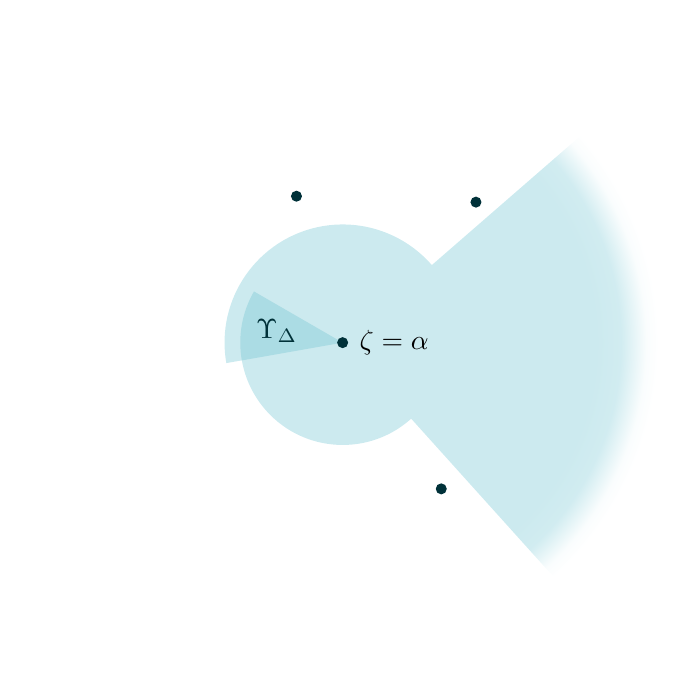
\begin{tikzpicture}
  \newcommand{\spill}{4}
  \fill[ietcoast!20, bezier bounding box, path fading=radial edge]
    (-\spill, -\spill) (\spill, \spill)
    (190:1.5) arc (190:41:1.5) -- (41:\spill) arc (41:-48:\spill) -- (-48:1.3) arc (-48:-170:1.3) -- cycle;
  \fill[ietcoast!33] (0, 0) -- (-170:1.3) arc (-170:-210:1.3) -- cycle;
  \fill[ietcoast!33!black] circle (0.7mm) node[anchor=west, black, outer sep=1mm] {$\zeta = \alpha$};
  \node[ietcoast!33!black] at (-190:0.85) {$\Upsilon_\Delta$};
  \foreach \p in {(107.5:1.95), (46.5:2.46), (-56:2.24)} {
    \fill[ietcoast!33!black] \p circle (0.7mm);
  }
\end{tikzpicture}
\end{center}
\color{HotPink}
For any $\sigma \in \R$, $\Lambda \in \R$, and non-integer $\rho \ge \sigma$, the intersection
\[ \zeta^\rho\,\mathcal{O}_{\zeta = 0} \cap \singexp{\sigma}{\Lambda}(\Upsilon) \]
\color{black}
\color{SteelBlue}
For any $\rho \in \R \smallsetminus \Z$, $\Lambda \in \R$ and $\sigma \in (\rho-1, \rho]$, the intersection
\[ \zeta^\rho\,\mathcal{O}(\pi \Upsilon) \cap \singexp{\sigma}{\Lambda}(\Upsilon) \]
\color{black}
is a closed subspace of $\singexp{\sigma}{\Lambda}(\Upsilon)$.
\end{lemma}
\begin{proof}
Each point $b \in \Upsilon_\Delta$ has two preimages $b_+, b_- \in \Upsilon$, where $b_+$ is $2\pi$ counterclockwise of $b_-$ around $\zeta = \alpha$. The {\em variation} operator $\var \maps \singexp{\sigma}{\Lambda}(\Upsilon) \to \singexp{\sigma}{\Lambda}(\Upsilon_\Delta)$, defined by\footnote{The target of the variation operator is a space of functions on $\Upsilon_\Delta$ because the variation is defined only on the overlap. Our notation follows the convention of \cite{diverg-resurg-i}, described before Definition~6.46.}
\[ \var \varphi \big|_b = \varphi(b_+) - \varphi(b_-) \]
is bounded. A function in $\singexp{\sigma}{\Lambda}(\Upsilon)$ descends and extends to a function on a neighborhood of $\zeta = 0$ in $\C$ if and only if it lies in the kernel of $\var - (e^{2\pi i \rho} - 1)$. This operator is bounderd, so its kernel is closed.
\end{proof}
\color{SteelBlue}
If a function in $\zeta^\rho\,\mathcal{O}(\pi \Upsilon)$ also belongs to $\singexp{\sigma}{\Lambda}(\Upsilon)$, its Laurent series cannot include any terms more singular than $\zeta^\sigma$. That means its Laurent series is actually a Taylor series.
\begin{prop}\label{prop:shifted_holo_series}
Under the conditions of Lemma~\ref{lem:shifted_holo_closed}, every function in
\[ \zeta^\rho\,\mathcal{O}(\pi \Upsilon) \cap \singexp{\sigma}{\Lambda}(\Upsilon) \]
is the sum of a shifted Taylor series in $\zeta^\rho\,\C\{\zeta\}$.
\end{prop}
\begin{proof}
Since $\pi \Upsilon$ contains a punctured disk around $\zeta = 0$, every function $\varphi \in \zeta^\rho\,\mathcal{O}(\pi \Upsilon)$ is the sum of a shifted Laurent series $\series{\varphi} \in \zeta^\rho\,\C\{\zeta, \zeta^{-1}\}$. The definition of $\singexp{\sigma}{\Lambda}(\Upsilon)$ tells us that $|\zeta|^\sigma |\varphi|$ is bounded on a punctured disk around $\zeta = 0$, which would be impossible if $\series{\varphi}$ included any $\zeta^{\rho-1},\;\zeta^{\rho-2},\;\zeta^{\rho-3}\ldots$ terms. That means $\series{\varphi}$ must belong to $\zeta^\rho\,\C\{\zeta\}$.
\end{proof}
\color{black}

Taylor expansion and summation form a two-way link between holomorphic functions and formal power series. For regular enough functions, the Laplace transform preserves a one-way vestige of this link: it turns Taylor expansions on the position domain into asymptotic expansions on the frequency domain. \begin{todo}[Compare with Sokal's version of the Watson--Nevanlinna theorem?]\end{todo}
\begin{lemma}\label{lem:laplace-bridge}
Let $\Omega$ be an open sector with $\zeta = 0$ at its tip, and an opening angle of $\pi$ or less. Take some $\rho \in (-1,\infty)$. If $\varphi \in \singexp{\rho}{\Lambda}(\Omega)$ is the sum of a power series $\series{\varphi} \in \zeta^\rho\,\C\{\zeta\}$, then its Laplace transform $\Phi = \laplace_{\zeta, 0}^\theta \varphi$ is asymptotic to the formal Laplace transform $\series{\Phi} = \laplace_{\zeta, 0} \series{\varphi}$. \textcolor{orange}{[Define formal Laplace transform into transmonomial spaces?]}
\end{lemma}
\begin{remark}
This result is similar to Theorem~5.20 of \cite{diverg-resurg-i}. It is weaker in that it does not establish Gevrey asymptoticity, but stronger in that it can be applied to functions with fractionally shifted Taylor expansions.
\end{remark}
\begin{proof}
By adding points within the disk around $\zeta = 0$ where $\series{\varphi}$ converges, expand $\Omega$ to an open set $\Upsilon \subset \widetilde{\C^\times}$ of the kind used in Lemma~\ref{lem:shifted_holo_closed}. Write $\series{\varphi}$ out in the form
\[ \series{\varphi} = a_0 \frac{\zeta^\rho}{\Gamma(\rho+1)} + a_1 \frac{\zeta^{\rho+1}}{\Gamma(\rho+2)} + a_2 \frac{\zeta^{\rho+2}}{\Gamma(\rho+3)} + a_3 \frac{\zeta^{\rho+3}}{\Gamma(\rho+4)} + \ldots, \]
observing that
\[ \series{\Phi} = \frac{a_0}{z^{\rho+1}} + \frac{a_1}{z^{\rho+2}} + \frac{a_2}{z^{\rho+3}} + \frac{a_3}{z^{\rho+4}} + \ldots. \]
For each $n \in \Z_{\ge 0}$, define the tail sum $\varepsilon_n \in \singexp{\sigma+n}{\Lambda}(\Upsilon)$ by the equation
\[ \varphi = a_0 \frac{\zeta^\rho}{\Gamma(\rho+1)} + a_1 \frac{\zeta^{\rho+1}}{\Gamma(\rho+2)} + \ldots + a_{n-1} \frac{\zeta^{\rho+n-1}}{\Gamma(\rho+n)} + \varepsilon_n. \]
Taking the Laplace transform of both sides, we learn that
\[ \Phi = \frac{a_0}{z^{\rho+1}} + \frac{a_1}{z^{\rho+2}} + \ldots + \frac{a_{n-1}}{z^{\rho+n}} + E_n, \]
where $E_n = \laplace_{\zeta, 0}^\theta \varepsilon_n$. To show that $\Phi$ is asymptotic to $\series{\Phi}$, we just need to prove that $|z^{\rho+n} E_n| \to 0$ as $|z| \to \infty$ along every ray.

Because of the conditions we put on $\Omega$, we can apply Proposition~\ref{prop:laplace-cont}, which tells us that $E_n$ lies in $\dualsingexp{-\rho-n-1}{\Lambda}(\widehat{\Omega}_0^\Lambda)$. This means that $|E_n| \lesssim \Delta^{-\rho-n-1}$, where $\Delta$ is the distance to the boundary of $\widehat{\Omega}_\alpha^\Lambda$. Noting that $|z|/\Delta$ goes to a constant limit as $z \to \infty$ along any ray \textcolor{magenta}{[check]},\footnote{The constant limit is not uniform over all rays, so we are showing that $\Phi$ is asymptotic, but not necessarily uniformly asymptotic, to $\series{\Phi}$.} we deduce that
\begin{align*}
|z^{\rho+n} E_n| & \lesssim |z|^{\rho+n} \Delta^{-\rho-n-1} \\
& = \big(|z|/\Delta\big)^{\rho+n} \Delta^{-1} \\
& \lesssim \Delta^{-1}
\end{align*}
along any ray. This, as discussed above, proves the desired result.
\end{proof}
\color{black}

%The space of $1$-Gevrey formal series is a $\C$-algebra with unit $1$, thus in order to prove that $\borel_\zeta$ is an algebra homomorphism between $\C\llbracket z^{-1}\rrbracket_1$ and $\C\lbrace\zeta\rbrace$ we should endow $\C\lbrace\zeta\rbrace$ with the convolution product and with the formal unit $\delta\defeq\borel_\zeta 1$. 

%Let $\tilde{\Phi}, \tilde{\Psi}\in \C \llbracket z^{-1} \rrbracket_1$ (where we assume they are series on the fiber over $\zeta=0$), then 
%\[\borel_\zeta(\tilde{\Psi}\tilde{\Phi})=:\tilde{\psi}\ast\tilde{\phi}.\]
%In addition, as proved in \cite[Definition 5.12 and Lemma 5.14]{diverg-resurg-i}, the convolution product $\ast$ can be explicitly characterized as \textcolor{orange}{[maybe just define it on holomorphic functions first, and then extend to all formal series by linearity via Taylor series]}
%\[
 %   \series{\psi}\ast\series{\phi}=\int_0^{\zeta}d\zeta' \series{\psi}(\zeta-\zeta')\series{\phi}(\zeta').
%\]
%\begin{lemma}
%The convolution product induces an algebra structure on the space $\singexp{\sigma}{\Lambda}(\Omega)$.
%\end{lemma}
%\begin{proof}
%    Let $\tilde{\phi},\tilde{\psi}\in\singexp{\sigma}{\Lambda}(\Omega)$, then a simple computation shows $\tilde{\phi}\ast\tilde{\psi}\in\singexp{\sigma}{\Lambda}(\Omega)$.
%\begin{verify}
 %   \begin{align*}
  %      | \tilde{\phi}\ast\tilde{\psi}|&=\left|\int_0^\zeta\tilde{\phi}(\zeta-\zeta')\tilde{\psi}(\zeta')\, d\zeta'\right|\\
   %     &\le \int_0^\zeta |\tilde{\phi}(\zeta-\zeta')||\tilde{\psi}(\zeta')|\, d\zeta'\\
    %    &\le ||\tilde{\psi}||_{\sigma,\Lambda} \int_0^\zeta\tilde{\phi}(\zeta-\zeta')|\zeta'|^{\sigma}e^{\Lambda|\zeta'|}\, d\zeta'\\
    %    &\le ||\tilde{\psi}||_{\sigma,\Lambda} |\zeta|^{\sigma}e^{\Lambda|\zeta|} \int_0^\zeta\tilde{\phi}(\zeta-\zeta')|\zeta-\zeta'|^{\sigma}e^{\Lambda|\zeta-\zeta'|}\, d\zeta'\\
    %    &\le |\zeta|^{\sigma}e^{\Lambda|\zeta|} ||\tilde{\psi}||_{\sigma,\Lambda} ||\tilde{\phi}||_{\sigma,\Lambda}. 
    %\end{align*}
%\end{verify}
%\end{proof}
%We deduce that also the Laplace transform is a $\C$-algebra homomorphism from $\singexp{\sigma}{\Lambda}(\Omega)$ to the space of holomorphic functions on $H_\theta$.  
%\begin{prop}
 %   Let $\sigma>-1$, $\Lambda>0$ and $\theta\in [0,2\pi)$. Then the Laplace transform $\laplace_{\zeta,0}^\theta$ is $\C$-algebra homomorphism from $\singexp{\sigma}{\Lambda}(\Omega)$ to $\mathcal{O}(H_\theta)$. 
%\end{prop}
%\begin{proof}
%First of all, from the properties of $\laplace_{\zeta,0}^\theta$ we know that if $\phi, \psi\in\singexp{\sigma}{\Lambda}(\Omega)$, then
%\[\laplace_{\zeta,0}^\theta\big[{\phi}\ast{\psi}\big]=\laplace_{\zeta,0}^\theta\big[{\phi}\big]\laplace_{\zeta,0}^\theta\big[{\psi}\big],\]
%see for instance \cite[Theorem 2.39]{laplace-tfm}. Then we should prove that $\delta$ is a unit: from its definition and the fact that $\borel_\zeta$ is the formal inverse of $\laplace_{\zeta,0}$, we deduce that 
 %   \[
%\laplace_{\zeta,0}^\theta\big[\delta\big]:=\laplace_{\zeta,0}^\theta\big[\borel_\zeta(1)\big]=1.
 %   \]
%Thus, $\delta$ behaves as a Dirac delta distribution acting on $\singexpalg{\sigma}(\Omega)$. Then, if ${\phi}\in\singexp{\sigma}{\Lambda}(\Omega)$
  %   \begin{align*}
%\big[\delta\ast\phi\big](p)&=\int_0^{\zeta(p)} \delta(\zeta(p)-\zeta)\phi(\zeta) \, d\zeta=\phi(p)
 %   \end{align*}
%\end{proof}
%
%
\subsection{Action on fractional derivatives and fractional integrals}\label{sec:frac-diff-laplace}
In this section, we will consider the action of $\borel_\zeta$ and $\laplace_{\zeta,0}$ with respect to the action of derivatives in both the frequency and position domains, as well as fractional integrals and derivatives $\fracderiv{\lambda}{\zeta}{0}$ in the position domain. This will be useful in Section~\ref{sec:examples}. 

In our treatmeant, we will restrict the Borel transform to the space of $1$-Gevrey series and the Laplace transform to $\singexp{\sigma}{\Lambda}$ \textcolor{magenta}{[needs domain]} with $\sigma>-1$ and $\Lambda>0$. 
\begin{definition}
For $\nu \in (-\infty, 1)$, the \textit{fractional integral} $\partial^{\nu-1}_{\zeta, \alpha}$ is defined by
\[ [\partial^{\nu-1}_{\zeta, \alpha} \phi](p) \defeq \frac{1}{\Gamma(1-\nu)} \int_{\zeta =\alpha}^p \big(\zeta(p)-\zeta\big)^{-\nu} \phi\,d\zeta, \]
where $p$ is any point on the position domain $B$.%\footnote{\textcolor{magenta}{Why highlight this special case of the definition above? Is it important to use $\lambda$ instead of $\nu-1$?} For completeness we also give the \textcolor{magenta}{[redundant] definition} of the fractional integral $\partial_{\zeta_\alpha,0}^{-\lambda}$: 
% \begin{equation*}
%     \partial_{\zeta_\alpha,0}^{-\lambda}\varphi(p)\defeq\frac{1}{\Gamma(\lambda)}\int_{\zeta_\alpha=0}^{p}(\zeta_\alpha(p)-\zeta_\alpha)^{\lambda-1} \varphi \, d\zeta_\alpha.
% \end{equation*}
% }
\end{definition}
The fractional integral obeys the expected semigroup law \cite[Section  1.3]{mladenov2014advanced}
\begin{align*}
\fracderiv{\lambda}{\zeta}{\alpha}\,\fracderiv{\mu}{\zeta}{\alpha} & = \fracderiv{\lambda+\mu}{\zeta}{\alpha} \qquad \lambda, \mu \in (-\infty, 0),
\end{align*}
and agrees with ordinary repeated integration when $\nu$ is an integer~\cite[Equation 35]{mladenov2014advanced}.

For $\mu \in (0, 1)$ and integers $n \ge 0$, fractional derivatives $\fracderiv{n+\mu}{\zeta}{0}$ are defined by composing $\fracderiv{\mu-1}{\zeta}{0}$ with powers of $\tfrac{\partial}{\partial \zeta}$. However, $\fracderiv{\mu-1}{\zeta}{0}$ and $\tfrac{\partial}{\partial \zeta}$ do not commute~\cite[equation 54]{mladenov2014advanced}. Various ordering conventions give various definitions of $\fracderiv{n+\mu}{\zeta}{0} \phi$, which differ by operators that act on the germ of $\phi$ at zero (see \cite[Section 1.3]{mladenov2014advanced}---original source \cite{podlubny}). We will use the {\em Riemann-Liouville} convention.
\begin{definition}\label{definition:frac_driv}
For $\mu \in (0, 1)$ and integers $n \ge 0$, the {\em Riemann-Liouville fractional derivative} $\fracderiv{n+\mu}{\zeta}{0}$ is defined by
\[ \fracderiv{n+\mu}{\zeta}{0} \defeq \big(\tfrac{\partial}{\partial \zeta}\big)^{n+1} \fracderiv{\mu-1}{\zeta}{0}. \]
\end{definition}
The symbol $\fracderiv{\mu}{\zeta}{0}$ is now defined for any $\mu \in \R \smallsetminus \{0, 1, 2, 3, \ldots\}$. It denotes a fractional integral when $\mu$ is negative, and a fractional derivative when $\mu$ is a positive non-integer.

The Riemann-Liouville fractional derivative is a left inverse of the fractional integral, in the sense that $\fracderiv{\lambda}{\zeta}{ 0}\,\fracderiv{-\lambda}{\zeta}{0}$ is the identity for all $\lambda \in (0, \infty)$. This extends the semigroup law:
\begin{align*}
\fracderiv{\lambda}{\zeta}{0}\,\fracderiv{\mu}{\zeta}{0} & = \fracderiv{\lambda+\mu}{\zeta}{0} & \lambda \in \R \smallsetminus \{0, 1, 2, 3, \ldots\},\quad\mu \in (-\infty, 0).
\end{align*}
\begin{prop}\label{prop:L-int-op}
Let $\phi\in\singexp{\sigma}{\Lambda}(\Omega)$ with $\sigma>-1$ and $\Lambda>0$, then
\begin{itemize}
\item[(i)] \emph{[fractional derivative]} for every $\mu\in(0,1)$, $\laplace_{\zeta,0} \big[\fracderiv{\mu}{\zeta}{0} \phi\big] = z^{\mu} \laplace_{\zeta,0} \phi$;
\item[(ii)] \emph{[fractional integral]} $\laplace_{\zeta,0} \big[\fracderiv{\lambda}{\zeta}{0} \phi\big] = z^{\lambda} \laplace_{\zeta,0} \phi$ for every $\lambda\in\R_{<0}$;
\item[(iii)] \emph{[derivative]} let $n\in\Z_{>0}$ and assume that $ \phi^{(k)}(0)=0$ for every $k=0,\ldots,n$. Then $\laplace_{\zeta,0} \big[\big(\frac{\partial}{\partial\zeta}\big)^n \phi\big] = z^{n} \laplace_{\zeta,0} \phi$;
\item[(iv)] $\laplace_{\zeta,0} \big[\zeta^n \phi\big] = \big(-\frac{\partial}{\partial z}\big)^n \laplace_{\zeta,0} \phi$, 
for every $n\in\Z_{\geq 0}$.
\end{itemize}
\end{prop}
\begin{proof}
%where in the last step we repetedly use integration by part and the fact that boundary terms vanish. %Then we deduce that   
%\begin{align*}
 %   z^\mu\laplace_{\zeta,0}\phi&= \laplace_{\zeta,0}\Big[\frac{\zeta^{-\alpha-1}}{\Gamma(-\alpha)}\Big] \laplace_{\zeta,0}\big[\partial_\zeta^n \phi\big]\\
  %  &=\laplace_{\zeta,0}\Big[\frac{\zeta^{-\alpha-1}}{\Gamma(-\alpha)}\ast \partial_\zeta^n\phi\Big]\\
   % &=z^n\laplace_{\zeta,0}\Big[\fracderiv{\lambda}{\zeta}{0}\partial_\zeta^n \phi\Big]
%\end{align*}
   
   The result of \emph{(i)} and \emph{(ii)} follow from the properties of the Laplace transform with respect to the convolution product: for every $\tau\in\R_{<0}\cup(0,1)$
    \begin{align*}
        z^\tau\laplace_{\zeta,0}\phi&=\laplace_{\zeta,0}\Big[\frac{\zeta^{-\tau-1}}{\Gamma(-\tau)}\Big] \laplace_{\zeta,0}\phi\\
        &=\laplace_{\zeta,0}\Big[\frac{\zeta^{-\tau-1}}{\Gamma(-\tau)}\ast \phi\Big]\\
        &=\laplace_{\zeta,0} \int_0^{\zeta}\frac{(\zeta-\zeta')^{-\tau-1}}{\Gamma(-\tau)} \phi(\zeta') d\zeta'\\
        &=\laplace_{\zeta,0}\fracderiv{\tau}{\zeta}{0}\phi
        \end{align*}
        The result of $(iii)$ follows by repetedly using integration by part and the fact that boundary terms vanish:
\begin{align*}
    z^n\laplace_{\zeta,0}\phi&=\int_0^\infty e^{-z\zeta} z^n \phi \, d\zeta\\
    &=(-1)^n\int_0^\infty \partial_\zeta^n \big[e^{-z\zeta}\big]  \phi\, d\zeta\\
    &=\laplace_{\zeta,0}\big[\partial_\zeta^n \phi\big].
\end{align*}
     Finally, the proof of $(iv)$ follows by integration by parts and the fact that $\zeta^n\phi\in\singexp{\sigma}{\Lambda}(\Omega)$.   
        %from a 2d integration argument, akin to the one in \cite[Theorem~2.39]{laplace-tfm}. This generalizes the Laplace transform's action on derivatives: using differentiation under the integral we prove \emph{ii)} (see also \cite[Theorem~1.34]{laplace-tfm}). Similarly, one can prove \emph{iii)}.  
\end{proof}
\begin{lemma}\label{lem:frac-deriv-Borel}
For any non-integer $\mu \in (0, \infty)$ and any integer $k \ge 0$,
\[ \partial^\mu_{\zeta } \borel_\zeta \big[z^{-(k+1)}\big] =  \borel_\zeta \big[z^\mu z^{-(k+1)}\big]. \]
\end{lemma}
\begin{proof}
We will show that for any $\mu \in (0, 1)$ and any integer $n \ge 0$, the claim holds with $\mu = n + \alpha$. First, evaluate
\begin{align*}
\partial^{\mu-1}_{\zeta} \borel_\zeta \big[z^{-(k+1)}\big] & = \frac{1}{\Gamma(1-\mu)} \int_0^\zeta (\zeta-\zeta')^{-\mu} \frac{{\zeta'}^k}{\Gamma(k+1)}\,d\zeta' \\
& = \frac{1}{\Gamma(1-\mu)\,\Gamma(k+1)} \int_0^1 (\zeta-\zeta t)^{-\mu} (\zeta t)^k\,\zeta\,dt \\
& = \frac{\zeta^{k-(\mu-1)}}{\Gamma(1-\mu)\,\Gamma(k+1)} \int_0^1 (1-t)^{-\mu} t^k\,dt \\
& = \frac{\zeta^{k-(\mu-1)}}{\Gamma\big(k-(\mu-1)+1\big)}
\end{align*}
by reducing the integral to Euler's beta function (see \cite[Identity 5.12.1]{dlmf}). This establishes that
\begin{equation}\label{frac-diff-laplace}
\big(\tfrac{\partial}{\partial \zeta}\big)^{n+1}\,\partial^{\mu-1}_{\zeta } \borel_\zeta \big[z^{-(k+1)}\big] = \frac{\zeta^{k-(n+\mu)}}{\Gamma\big(k-(n+\mu)+1\big)}
\end{equation}
for $n = -1$. If \eqref{frac-diff-laplace} holds for $n = m$, it also holds for $n = m+1$, because
\begin{align*}
\tfrac{\partial}{\partial \zeta} \big(\tfrac{\partial}{\partial \zeta}\big)^{m+1}\,\partial^{\mu-1}_{\zeta} \borel_\zeta \big[z^{-(k+1)}\big] & = \frac{\partial}{\partial \zeta} \left( \frac{\zeta^{k-(m+\mu)}}{\big(k-(m+\mu)\big)\,\Gamma\big(k-(m+\mu)\big)} \right) \\
& = \frac{\zeta^{k-(m+1+\mu)}}{\Gamma\big(k-(m+\mu)\big)}
\end{align*}
Hence, \eqref{frac-diff-laplace} holds for all $n \ge -1$, and the desired result quickly follows. The condition $\mu \in (0, 1)$ saves us from the trouble we would run into if $k-(m+\mu)$ were in $\Z_{\le 0}$. This is how we avoid the initial value corrections that appear in ordinary derivatives of Borel transforms.
\end{proof}
We can now prove the properties of the Borel transform analogous to the one of the Laplace transform from Proposition~\ref{prop:L-int-op}.
\begin{prop}\label{prop:frac-der-int-borel}
Let $\tilde{\Phi}\in\C\llbracket z^{-1}\rrbracket_1$ %and let $\hat{\phi}$ be the sum of $\borel_\zeta\tilde{\Phi}$, then %and $\tilde{\phi}\defeq\borel_\zeta\tilde{\Phi}$
\begin{itemize}
\item[(i)] \emph{[fractional derivative]} $\borel_\zeta\big[ z^\mu \, \tilde{\Phi}\big]=\fracderiv{\mu}{\zeta}{0}\, \borel_\zeta\series{\Phi}$, for every $\mu\in\R_{> 0}$;
\item[(ii)] \emph{[fractional integral]} $\borel_\zeta\big[z^\lambda\, \tilde{\Phi}\big]=\fracderiv{\lambda}{\zeta}{0}\,\borel_\zeta\series{\Phi}$, for every $\lambda\in\R_{<0}$; 
\item[(iii)] let $k\in\Z_{\ge 0}$ and $\tilde{\Phi}\in z^{-k-1}\llbracket z^{-1}\rrbracket_1$, then $\borel_\zeta\big[\partial_z^{k} \tilde{\Phi}\big]=(-\zeta)^k\borel_\zeta\tilde{\Phi}$.\footnote{This property holds more generally for $\tilde{\Phi}\in\C\llbracket z^{-1}\rrbracket$, without restricting to $1$-Gevrey series.}
\end{itemize} 
\end{prop}
\begin{proof} 
The proof of $(i)$ follows from Lemma \ref{lem:frac-deriv-Borel}. 

Then, to prove $(ii)$, first notice that for $\lambda\in\R_{< 0}$  
\[\fracderiv{\lambda}{\zeta}{0}\zeta^{k}=\zeta^{k-\lambda}\frac{k!}{\Gamma(k-\lambda+1)}.\] 
Hence, if $\tilde{\Phi}=\sum_{n\geq 0}a_n z^{-n}$ %and $\hat{\phi}$ denotes the sum of $\borel_\zeta\tilde{\Phi}$
\[\borel_\zeta \big[z^\lambda \tilde{\Phi}\big]=\sum_{n\geq 0}a_n\frac{\zeta^{n-\lambda}}{\Gamma(n-\lambda+1)}=\sum_{n\geq 0}a_n\frac{\zeta^{n-\lambda}}{n!}\frac{n!}{\Gamma(n-\lambda+1)}=\sum_{n\geq 0} \frac{a_n}{n!}\,\fracderiv{\lambda}{\zeta}{0}\zeta^n=\fracderiv{\lambda}{\zeta}{0}\series{\Phi}\]
where in the last step, we use that $\borel_\zeta\tilde{\Phi}$ is convergent. 

Finally, $(iii)$ follows from a simple computation: 
\begin{align*}
\borel_\zeta\big[\partial_z^k\tilde{\Phi}\big]&=\borel_\zeta\left[\sum_{n=k+1}^\infty a_n \frac{(n+k-1)!}{(n-1)!} (-1)^{k} z^{-n-k}\right]\\
&=(-1)^k \sum_{n=k+1}^\infty a_n \frac{(n+k-1)!}{(n-1)!}\frac{\zeta^{n+k-1}}{(n+k-1)!}\\
&=(-\zeta)^k\sum_{n=k+1}^\infty a_n \frac{\zeta^{n-1}}{(n-1)!}\\
&=(-\zeta)^k\borel_\zeta \tilde{\Phi}
\end{align*}
\end{proof}
% \begin{remark}
% We notice that properties $(i)$ and $(ii)$ of Proposition~\ref{prop:frac-der-int-borel} are special cases of the convolution product: for every $\lambda\in\R\setminus\Z_{>0}$ 
% \[\fracderiv{\lambda}{\zeta}{0}\big[\borel_\zeta\tilde{\Phi}\big]=\borel_\zeta \big[z^\lambda \tilde{\Phi}\big]=\borel_\zeta (z^\lambda)\ast \borel_\zeta\tilde{\Phi}.\]
% \begin{verify}
% \begin{align*}
% \fracderiv{\tau}{\zeta}{0}\borel_\zeta\tilde{\Phi}=\borel_\zeta (z^\tau \tilde{\Phi})&=\borel_\zeta (z^\tau)\ast \borel_\zeta\tilde{\Phi}\\
% &=\frac{\zeta^{-\tau-1}}{\Gamma(-\tau)}\ast\sum_{n=0}^\infty a_n \frac{\zeta^n}{n!}\\
% &=\int_0^\zeta \frac{(\zeta')^{-\tau-1}}{\Gamma(-\tau)}\sum_{n= 0}^\infty a_n\frac{(\zeta-\zeta')^n}{n!}d\zeta'\\
% &=\sum_{n= 0}^\infty\frac{a_n}{n!}\frac{1}{\Gamma(-\tau)}\zeta^{n-\tau}\frac{\Gamma(n+1)\Gamma(-\tau)}{\Gamma(n-\tau+1)}
% \end{align*}
% Recall from Lemma~\ref{lem:frac-deriv-Borel} that for every 
% $\tau>0$ and $\tau\notin\Z_{>0}$, 
% \[\frac{\zeta^{n-\tau}}{\Gamma(n-\tau+1)}=\fracderiv{\tau}{\zeta}{0}\Big[\frac{\zeta^n}{n!}\Big]
% \]
% and if $\tau<0$, by definition 
% \[\fracderiv{\tau}{\zeta}{0}\Big[\frac{\zeta^n}{n!}\Big]=\frac{1}{\Gamma(-\tau)}\int_0^\zeta (\zeta')\frac{(\zeta-\zeta')^n}{n!}d\zeta'\]
% therefore, we deduce $\fracderiv{\tau}{\zeta}{0}\borel_\zeta\tilde{\Phi}=\frac{\zeta^{\tau-1}}{\Gamma(-\tau)}\ast\borel_\zeta\tilde{\Phi}$. 
% \end{verify}
% \end{remark}
\color{RoyalBlue}
We can express the fractional integrals/derivatives $\fracderiv{\lambda}{\zeta}{\alpha}$ as convolution product.
\begin{lemma}
    Let us assume $\Phi=\laplace_{\zeta,\alpha}\phi$ for $\phi\in\singexpalg{\sigma}(\Omega_\alpha)$, and $z$ to be a function on $T^*_{\zeta=0}B$. Then, for every $\lambda\in (-1,\infty)$
    \[\borel_\zeta (z^{-\lambda})\ast_{\zeta,\alpha}\borel_\zeta{\Phi}=\fracderiv{-\lambda}{\zeta}{\alpha}\big[\borel_\zeta\Phi\big].\]
\end{lemma}
\begin{proof}
    First of all, notice that 
    \begin{align*}
    \borel_\zeta(z^{-\lambda}{\Phi})=\borel_\zeta(z^{-\lambda}\laplace_{\zeta,\alpha}\phi)=\borel_\zeta(\laplace_{\zeta,\alpha}\partial_{\zeta,\alpha}^{-\lambda}\phi)=\partial_{\zeta,\alpha}^{-\lambda}\phi%=\frac{1}{\Gamma(\lambda)}\int_{\zeta=\alpha}^p (\zeta(p)-\zeta)^{\lambda-1}\phi d\zeta=\borel_\zeta (z^{-\lambda})\ast_{\zeta,\alpha}\phi
\end{align*}
where we use the identity $\laplace_{\zeta, \alpha}\,\fracderiv{-\lambda}{\zeta}{\alpha} \varphi = z^{-\lambda} \laplace_{\zeta, \alpha} \varphi$, that generalizes properties $(i)$ and $(ii)$ in Proposition~\ref{prop:L-int-op}. Then, by definition of fractional integral $\partial_{\zeta,\alpha}^{-\lambda}\phi$, we have
\begin{align*}
    \Big[\partial_{\zeta,\alpha}^{-\lambda}\phi\Big](p)=\frac{1}{\Gamma(\lambda)}\int_{\zeta=\alpha}^p (\zeta(p)-\zeta)^{\lambda-1}\phi\, d\zeta=\frac{1}{\Gamma(\lambda)}\int_{\zeta=\alpha}^p \mathsf{R}^{*}\zeta^{\lambda-1}\phi\, d\zeta=\borel_\zeta (z^{-\lambda})\ast_{\zeta,\alpha}\phi\,.
\end{align*}
\end{proof}
\begin{remark}
    
\end{remark}
% We first assume $\Phi=\laplace_{\zeta,\alpha}\phi$ for $\phi\in\singexpalg{\sigma}(\Omega_\alpha)$, and assume $z$ is a function on $T^*_{\zeta=0}B$. Then, for every $\lambda\in (-1,\infty)$
% \begin{align*}
%     \borel_\zeta(z^{-\lambda}{\Phi})=\borel_\zeta(z^{-\lambda}\laplace_{\zeta,\alpha}\phi)=\borel_\zeta(\laplace_{\zeta,\alpha}\partial_{\zeta,\alpha}^{-\lambda}\phi)=\partial_{\zeta,\alpha}^{-\lambda}\phi%=\frac{1}{\Gamma(\lambda)}\int_{\zeta=\alpha}^p (\zeta(p)-\zeta)^{\lambda-1}\phi d\zeta=\borel_\zeta (z^{-\lambda})\ast_{\zeta,\alpha}\phi
% \end{align*}
% where we use the identity $\laplace_{\zeta, \alpha}\,\fracderiv{-\lambda}{\zeta}{\alpha} \varphi = z^{-\lambda} \laplace_{\zeta, \alpha} \varphi$, that generalizes properties $(i)$ and $(ii)$ in Proposition~\ref{prop:L-int-op}. Then, by definition of fractional integral $\partial_{\zeta,\alpha}^{-\lambda}\phi$, we have
% \begin{align*}
%     \borel_\zeta(z^{-\lambda}{\Phi})(p)=\frac{1}{\Gamma(\lambda)}\int_{\zeta=\alpha}^p (\zeta(p)-\zeta)^{\lambda-1}\phi\, d\zeta=\borel_\zeta (z^{-\lambda})\ast_{\zeta,\alpha}\phi\,.
% \end{align*}
% Hence \[\borel_\zeta (z^{-\lambda})\ast_{\zeta,\alpha}\borel_\zeta{\Phi}=\fracderiv{-\lambda}{\zeta}{\alpha}\big[\borel_\zeta\Phi\big].\]
% %However, if we consider a different fiber on $T^*B$, we have to modify the definition of convolution product in order to generalize properties (i) and (ii): indeed assuming $\series{\Phi}=\laplace_{\zeta_\alpha,0}\phi$ we have for every $\lambda\in (0,\infty)$
% Then, we study the case when $\Phi$ and $z$ are functions on the fiber over $\zeta=b$, and we assume $\Phi=\laplace_{\zeta_b,0}\phi$ for $\phi\in\singexpalg{\sigma}(\Omega_b)$. For every $\lambda\in (-1,\infty)$
% \begin{multline*}
%     \borel_{\zeta_b}\big[z^{-\lambda}\Phi\big]=\borel_{\zeta_b}\big[z^{-\lambda}\laplace_{\zeta_b,0}\phi\big]=\borel_{\zeta_b}\big[\laplace_{\zeta_b,0}\partial_{\zeta_b,0}^{-\lambda}\phi\big]=\partial_{\zeta_b,0}^{-\lambda}\phi=\frac{1}{\Gamma(\lambda)}\int_{0}^{\zeta_b} (\zeta_b-t)^{\lambda-1}\phi(t)dt\\
%     =\borel_{\zeta_b}(z^{-\lambda})\ast\phi
% \end{multline*}
% hence,  \[\partial_{\zeta_b,0}^{-\lambda}\big[\borel_{\zeta_b}\Phi\big]=\borel_{\zeta_b} (z^{-\lambda})\ast\borel_{\zeta_b}{\Phi}.\]
%
%
%
\color{black}
\section{Proof of main results}\label{sec:proof_main_results}
%
\subsection{Borel regularity for ODEs}\label{borel_reg-ODE}
\color{NavyBlue}
\textcolor{PaleVioletRed}{[Revised flavor text.]}
In Section~\ref{sec:regularity-results}, we show that linear level~1 ODEs of a certain form always have Borel regular solutions, indexed by the characteristic roots of their constant-coefficient parts. These solutions turn out to be asymptotic to the formal series solutions found by Poincar\'{e}.

In Section~\ref{sec:new-summability-proof}, we will look at the same class of ODEs from a more formal perspective, starting from the assumption that Poincar\'{e}'s solutions exist and are $1$-Gevrey. Using the existence and uniqueness results that characterize the Borel regular solutions, we give a new proof that Poincar\'{e}'s solutions are Borel summable.
\color{black}
\subsubsection{Regularity results}\label{sec:regularity-results}
Let us recall the setting from Section~\ref{borel-reg:explanatory-power}. Let $\mathcal{P}$ be a linear differential operator of the form \textcolor{PaleVioletRed}{[I just noticed we use $\partial_z$ instead of $\tfrac{\partial}{\partial z}$ in \texttt{reg-sing-volterra}, where these equations were copied from. Could we switch to $\tfrac{\partial}{\partial z}$, as I've done provisionally?]}
\begin{equation}\label{eqn:operator-P}
\mathcal{P} = P\big(\tfrac{\partial}{\partial z}\big) + \frac{1}{z} Q\big(\tfrac{\partial}{\partial z}\big) + \frac{1}{z^2} R(z^{-1}),
\end{equation}
where
\begin{enumerate}
\item $P$ is a monic degree-$d$ polynomial whose roots are all simple; 
\item $Q$ is a degree-$(d-1)$ polynomial that is non-zero at every root of $P$;
\item $R(z^{-1})$ is holomorphic in some disk $|z| > A$ around $z = \infty$. In particular, the power series
\[ R(z^{-1}) = \sum_{j=0}^\infty R_j z^{-j} \]
converges in the region $|z| > A$.
\end{enumerate}
%%For each root $-\alpha$ of $P$, choose an open sector $\Omega_\alpha \subset \C$ that has $\zeta = \alpha$ at its tip, does not touch any other root of $P(-\zeta)$, and has an opening angle of $\pi$ or less.
\textcolor{orange}{[Introduce $\hat{\mathcal{P}}_\alpha$?]} \textcolor{orange}{[Transition text]}
%%%\begin{itemize}
%%%\item The set $\Omega_\alpha$ is star-shaped around $\zeta = \alpha$. In other words, for any $a \in \Omega_\alpha$, a straight path from $\zeta = \alpha$ to $a$ stays in $\Omega_\alpha$. Since $\Omega_\alpha$ does not contain $\zeta = \alpha$, we will always leave that starting point out of the path.
%%%\item The set $\Omega_\alpha$ does not contain the tubular neighborhood of the other critical points, as shown in Figure \ref{Fig:domain}. \textcolor{orange}{[In ``Regular singular Volterra,'' we assume that $\Omega_\alpha$ does not touch any other critical point (that is, does not contain any other critical point in its closure). Under the star-shaped assumption, I think that implies avoiding tubular neighborhoods of the shadow rays.]}
%%%\end{itemize}
\begin{theorem}[restatement of \ref{thm:exist_uniq_ODE}]\label{re:thm:exist_uniq_ODE}
Choose a root $-\alpha$ of $P$. Choose an open sector $\Omega_\alpha$ which has an opening angle of $\pi$ or less, has $\zeta = \alpha$ at its tip, and does not touch any other root of $P(-\zeta)$. The equation $\mathcal{P}\Psi = 0$ has a unique solution $\Psi_\alpha$ in the affine subspace \textcolor{orange}{[define $\widehat{\Omega}_\alpha$]}
\[ e^{-\alpha z} \left[ z^{-\tau_\alpha} + \dualsingexpalg{-\tau_\alpha-1}(\widehat{\Omega}_\alpha) \right] \]
of the space $e^{-\alpha z} \dualsingexpalg{-\tau_\alpha}(\widehat{\Omega}_\alpha)$ from Section~\ref{sec:reg-decay}.
\end{theorem}
\begin{center}
%\begin{figure}
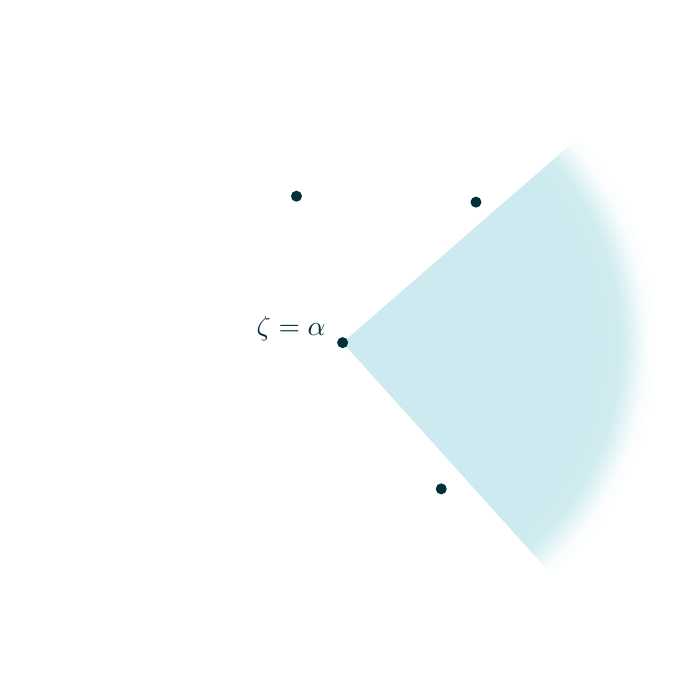
\begin{tikzpicture}
\newcommand{\spill}{4}
\fill[ietcoast!20, bezier bounding box, path fading=radial edge]
  (-\spill, -\spill) (\spill, \spill)
  (0, 0) -- (41:\spill) arc (41:-48:\spill) -- cycle;
\fill[ietcoast!33!black] circle (0.7mm) node[anchor=-15, outer sep=1mm] {$\zeta = \alpha$};
\foreach \p in {(107.5:1.95), (46.5:2.46), (-56:2.24)} {
  \fill[ietcoast!33!black] \p circle (0.7mm);
}
\end{tikzpicture}

{\small The domain $\Omega_\alpha$ \textcolor{orange}{[Cite as ``the figure after Lemma~***]}}
%\end{figure}
\end{center}
\begin{proof}
After rescaling by a constant, Theorem~4 of \cite{reg-sing-volterra} tells us that the equation $\hat{\mathcal{P}}_\alpha \psi_\alpha = 0$ has a unique solution $\psi_\alpha$ in the affine subspace
\[ \frac{\zeta^{\tau_\alpha-1}}{\Gamma(\tau_\alpha)} + \singexpalg{\tau_\alpha}(\Omega_\alpha) \]
of the space $\singexpalg{\tau_\alpha-1}(\Omega_\alpha)$. The same is true on any smaller sector created by shaving a sector off each edge of $\Omega_\alpha$. By Theorem~\ref{translation} and the results of Section~\ref{sec:reg-decay}, the Laplace transform $\laplace^\theta_{\zeta, \alpha}$ is a left-invertible map
\[ \singexpalg{\tau_\alpha}(\Omega_\alpha) \to e^{-\alpha z} \dualsingexpalg{-\tau_\alpha-1}(\widehat{\Omega}_\alpha). \]
With $\Psi_\alpha = \laplace^\theta_{\zeta, \alpha} \psi_\alpha$, the desired result follows.
\end{proof}
\color{RoyalBlue}
\textcolor{orange}{[\ldots]} Our arguments in \cite{reg-sing-volterra} took place on $\C$, but they work just as well on a covering of $\C$ which is branched at the roots of $P(-\zeta)$. Let us use the covering $\pi \maps \widetilde{B}_{P(-\zeta)} \to \C$ built by puncturing $\C$ at the roots of $P(-\zeta)$, taking the universal cover, and then gluing the roots back in as infinite-order branch points.
\color{black}
\textcolor{orange}{[Add flavor text]}
\begin{theorem}[restatement of \ref{thm:soln_is_Borel_sum}]\label{re:thm:soln_is_Borel_sum}
The analytic solution $\Psi_\alpha$ from Theorem~\ref{thm:exist_uniq_ODE} is the Borel sum of a formal trans-monomial solution $\series{\Psi}_\alpha \in e^{-\alpha z} z^{-\tau_\alpha}\,\C \llbracket z^{-1} \rrbracket$ of the equation $\mathcal{P}\series{\Phi} = 0$.
\end{theorem}
\begin{proof}
Take an open sector $\Omega_\alpha$ of the kind used in Theorem~\ref{re:thm:exist_uniq_ODE}, and expand it to an open set $\Upsilon \subset \widetilde{\C^\times}$ of the kind used in Lemma~\ref{lem:shifted_holo_closed}. By Theorem~4 of \cite{reg-sing-volterra}, the equation $\hat{\mathcal{P}}_\alpha \psi_\alpha = 0$ has a unique solution $\psi_\alpha$ in the affine subspace \textcolor{orange}{[use $\zeta_\alpha$ in place of $\zeta$ throughout proof]}
\[ \frac{\zeta_\alpha^{\tau_\alpha-1}}{\Gamma(\tau_\alpha)} + \singexpalg{\tau_\alpha}(\Upsilon) \]
of the space $\singexpalg{\tau_\alpha-1}(\Upsilon)$. Restricting this solution to $\Omega_\alpha$ gives the analogous solution from the proof of Theorem~\ref{re:thm:exist_uniq_ODE}, as we can see from the uniqueness part of Theorem~4 of \cite{reg-sing-volterra}. To express $\Psi_\alpha = \laplace_{\zeta, \alpha} \psi_\alpha$ as the Borel sum of a trans-monomial, we first need to expess $\psi_\alpha$ as the sum of a convergent power series. We will do this by showing that $\psi_\alpha$ lies in $\zeta^{\tau_\alpha - 1}\,\mathcal{O}(\pi \Upsilon)$.

For convenience, let $p = P(-\zeta)$ and $q = Q(-\zeta)$. To prove Theorem~4 in \cite{reg-sing-volterra}, we rewrite the equation $\hat{\mathcal{P}}_\alpha \solwhole = 0$ as a regular singular Volterra equation $\solwhole = \volterra^\alpha \solwhole$ that satisfies the conditions of the underlying existence and uniqueness result~\cite[Theorem~3]{reg-sing-volterra}. The operator $\volterra^\alpha$ is the sum of the ``prototypical'' part
%%\[ \hardpart^\alpha = -\tfrac{1}{P(-\zeta)} \circ \partial^{-1}_{\zeta, \alpha} \circ Q(-\zeta) \]
\[ \hardpart^\alpha = -\tfrac{1}{p} \circ \partial^{-1}_{\zeta, \alpha} \circ q \]
and the perturbation
%%\[ \softpart^\alpha = \tfrac{1}{P(-\zeta)} \circ \partial^{-2}_{\zeta, \alpha} \circ R(\partial^{-1}_{\zeta, \alpha}) \]
\[ \softpart^\alpha = \tfrac{1}{p} \circ \partial^{-2}_{\zeta, \alpha} \circ R\big(\partial^{-1}_{\zeta, \alpha}\big). \]

Let us run through the proof of Theorem~3, specialized to the case we consider in Theorem~4. First, picking an arbitrary point $b \in \Omega_\alpha$, we show that the {\em prototype solution}
\[ \solproto(a) = \frac{1}{p(a)} \exp\left(-\int_{b}^{a}\frac{q}{p}\;d\zeta\right) \]
lies in the space $\singexpalg{\tau_\alpha - 1}(\Upsilon)$ and satisfies the equation $\solproto = \hardpart^\alpha \solproto$. We then look for a perturbation $\solptb$ that makes $\solwhole = \solproto + \solptb$ a solution of the Volterra equation we are trying to solve. This is equivalent to solving the inhomogeneous equation
\begin{equation}\label{eqn:inhomog-volterra}
\solptb = \softpart^\alpha \solproto + \volterra^\alpha \solptb
\end{equation}
The central idea of the proof is to show that $\softpart^\alpha$ maps $\solproto$, and in fact all of $\singexpalg{\tau_\alpha - 1}(\Upsilon)$, into $\singexpalg{\tau_\alpha}(\Upsilon)$, and that $\volterra^\alpha$ is a contraction of $\singexp{\tau_\alpha}{\Lambda}(\Upsilon)$ when $\Lambda$ is large enough. It follows, by the contraction mapping theorem, that equation~\eqref{eqn:inhomog-volterra} has a unique solution $\solptb$ in $\singexp{\tau_\alpha}{\Lambda}(\Upsilon)$. More explicitly, we can solve equation~\eqref{eqn:inhomog-volterra} by fixed-point iteration. Defining
\begin{align*}
\solptb^{(0)} & = \softpart^\alpha \solproto \\
\solptb^{(1)} & = \softpart^\alpha \solproto + \volterra^\alpha \solptb^{(0)} \\
\solptb^{(2)} & = \softpart^\alpha \solproto + \volterra^\alpha \solptb^{(1)} \\
\solptb^{(3)} & = \softpart^\alpha \solproto + \volterra^\alpha \solptb^{(2)} \\
& \;\;\vdots
\end{align*}
we get a sequence of functions that converges in $\singexp{\tau_\alpha}{\Lambda}(\Upsilon)$ to a solution $f_*$.

In \citesection{sec:construction} Section~3.2.1 of \cite{reg-sing-volterra}, we rewrite the prototype solution in the form
\[ \solproto(a) = \frac{1}{p(a)} \left(\frac{\zeta_\alpha(a)}{\zeta_\alpha(b)}\right)^{\tau_\alpha} \exp\left[-\int_b^a \left( \frac{q}{p} + \frac{\tau_\alpha}{\zeta_\alpha} \right)\;d\zeta_\alpha\right], \]
\textcolor{HotPink}{which shows that it represents a germ in $\zeta_\alpha^{\tau_\alpha-1}\,\mathcal{O}_{\zeta = \alpha}$.}
\textcolor{SteelBlue}{which shows that it lies in $\zeta_\alpha^{\tau_\alpha - 1}\,\mathcal{O}(\pi \Upsilon)$}. By working with Taylor series, we can show that $\softpart^\alpha$ maps
\textcolor{HotPink}{\[ \zeta_\alpha^{\tau_\alpha-1}\,\mathcal{O}_{\zeta=\alpha} \to \zeta^{\tau_\alpha}\,\mathcal{O}_{\zeta=\alpha} \]}
\textcolor{SteelBlue}{\[ \zeta^{\tau_\alpha-1}\,\mathcal{O}(\pi \Upsilon) \to \zeta^{\tau_\alpha}\,\mathcal{O}(\pi \Upsilon) \]}
and $\volterra^\alpha$ maps \textcolor{HotPink}{$\zeta_\alpha^{\tau_\alpha}\,\mathcal{O}_{\zeta=\alpha}$} \textcolor{SteelBlue}{$\zeta^{\tau_\alpha}\,\mathcal{O}(\pi \Upsilon)$} to itself. It follows that the sequence $\solptb^{(0)}, \solptb^{(1)}, \solptb^{(2)}, \ldots$ lies in \textcolor{HotPink}{$\zeta_\alpha^{\tau_\alpha}\,\mathcal{O}_{\zeta=\alpha} \cap \singexp{\tau_\alpha}{\Lambda}(\Upsilon)$} \textcolor{SteelBlue}{$\zeta^{\tau_\alpha}\,\mathcal{O}(\pi \Upsilon) \cap \singexp{\tau_\alpha}{\Lambda}(\Upsilon)$}, which by Lemma~\ref{lem:shifted_holo_closed} is a closed subspace of $\singexp{\tau_\alpha}{\Lambda}(\Upsilon)$. The limit $f_*$, which satisfies equation~\eqref{eqn:inhomog-volterra}, therefore \textcolor{HotPink}{represents a germ in $\zeta_\alpha^{\tau_\alpha}\,\mathcal{O}_{\zeta = \alpha}$} \textcolor{SteelBlue}{lies in $\zeta^{\tau_\alpha}\,\mathcal{O}(\pi \Upsilon)$}. Recalling that the prototype solution \textcolor{HotPink}{represents a germ in $\zeta_\alpha^{\tau_\alpha-1}\,\mathcal{O}_{\zeta = \alpha}$} \textcolor{SteelBlue}{lies in $\zeta^{\tau_\alpha - 1}\,\mathcal{O}(\pi \Upsilon)$}, we can deduce that $\psi_\alpha$ \textcolor{HotPink}{represents a germ in $\zeta_\alpha^{\tau_\alpha-1}\,\mathcal{O}_{\zeta = \alpha}$.} \textcolor{SteelBlue}{lies in that space} too.

\textcolor{HotPink}{We now cross over into the formal world, expanding $\psi_\alpha$ as} \textcolor{SteelBlue}{We now cross over into the formal world using Proposition~\ref{prop:shifted_holo_series}, which tells us that $\psi_\alpha$ is the sum of} a shifted Taylor series $\series{\psi}_\alpha \in \zeta_\alpha^{\tau_\alpha-1}\,\C\{\zeta\}$. By definition, the formal Laplace transform $\series{\Psi}_\alpha = \laplace_{\zeta, \alpha} \series{\psi}_\alpha$ lies in $e^{-\alpha z} z^{-\tau_\alpha}\,\C \llbracket z^{-1} \rrbracket$.

When we take the Borel sum of $\series{\Psi}_\alpha$, we start by retracing the construction steps described above. The Borel transform inverts the formal Laplace transform, bringing us back to $\series{\psi}_\alpha$, and summation then inverts the Taylor expansion, bringing us back to $\psi_\alpha$. We finish the Borel summation by taking the Laplace transform $\laplace^\theta_{\zeta, \alpha} \psi_\alpha$, giving $\Psi_\alpha$ by definition.
\end{proof}
\textcolor{orange}{[Add flavor text]}
\begin{theorem}[restatement of \ref{thm:soln_is_asymptotic}]\label{re:thm:soln_is_asymptotic}
\textcolor{magenta}{[revise organiztion to match intro]} The analytic solution $\Psi_\alpha$ from Theorem~\ref{re:thm:exist_uniq_ODE} is asymptotic to the formal solution $\series{\Psi}_\alpha$ from Theorem~\ref{re:thm:soln_is_Borel_sum}.
\end{theorem}
\begin{proof}
In the proof of Theorem~\ref{re:thm:soln_is_Borel_sum}, we showed that the position-domain solution $\psi_\alpha \in \singexpalg{\tau_\alpha-1}(\Upsilon)$ is the sum of a shifted Taylor series $\series{\psi}_\alpha \in \zeta^{\tau_\alpha-1}\,\C\{\zeta\}$. Since $\Psi_\alpha$ is the Laplace transform of $\psi_\alpha$, and $\series{\Psi}_\alpha$ is the formal Laplace transform of $\series{\psi}_\alpha$, the desired result follows from Lemma~\ref{lem:laplace-bridge}.
\end{proof}
%
\subsubsection{A new proof of the Borel summability of the Poincar\'{e} solutions}\label{sec:new-summability-proof}
%
In~\cite{int-irreg}, Poincar\'{e} described a formal way to solve the equation $\mathcal{P}\series{\Phi} = 0$ for an operator of the form~\eqref{eqn:operator-P}. Choose a root $-\alpha$ of $P$, set $\tau_\alpha = Q(-\alpha)/P'(-\alpha)$, and look for a formal solution $\series{\Psi}_\alpha$ in the space $e^{-z\alpha} z^{-\tau_\alpha}\C\llbracket z^{-1} \rrbracket$. Once the leading coefficient of $\series{\Psi}_\alpha$ is chosen, the rest of the coefficients are determined, and can be found order by order. The Ramis Index Theorem guarantees that $\series{\Psi}_\alpha$ will be $1$-Gevrey~\cite{ramis_index}.

We have come this far in our discussion of Poincar\'{e}'s method through formal reasoning in the frequency domain. From here, there are various ways to show that $\series{\Psi}_\alpha$ is Borel summable. We do it by using Theorem~4 of \cite{reg-sing-volterra} to show that the relevant integral equation in the position domain has a unique analytic solution.
\begin{theorem}\label{thm:summability_ODE}
Choose a root $-\alpha$ of $P$. Choose an open sector $\Omega_\alpha$ which has an opening angle of $\pi$ or less, has $\zeta = \alpha$ at its tip, and does not touch any other root of $P(-\zeta)$. If a $1$-Gevrey trans-monomial \textcolor{orange}{[define]} $\series{\Psi}_\alpha \in e^{-z\alpha} z^{-\tau_\alpha}\C\llbracket z^{-1} \rrbracket_1$ satisfies the equation $\mathcal{P} \series{\Psi}_\alpha = 0$, then it is Borel summable at $\alpha$ along any ray in $\Omega_\alpha$, and its Borel sum is proportional to the analogous analytic solution $\Psi_\alpha$ from Theorem~\ref{re:thm:exist_uniq_ODE}.
\end{theorem}
\begin{proof}
By Proposition~\ref{prop:frac-der-int-borel}, the Borel transform $\series{\psi}_\alpha = \borel_\zeta \series{\Psi}_\alpha$ is a formal solution of the equation $\hat{\mathcal{P}}_\alpha \series{\psi}_\alpha = 0$, where $\hat{\mathcal{P}}_\alpha$ is the operator described in equation~\textcolor{magenta}{\textbf{(?)}}. By Proposition~\ref{prop:gevrey_to_convergent}, the series $\series{\psi}_\alpha$ converges to a holomorphic function $\hat{\psi}_\alpha$ on some open set $\Omega_\text{near}$ created by restricting $\Omega_\alpha$ to a small disk around of $\zeta = \alpha$. Since the integrals in $\hat{\mathcal{P}}_\alpha \hat{\psi}_\alpha$ converge absolutely, $\hat{\psi}_\alpha$ satisfies the same equation that its Taylor series does: $\hat{\mathcal{P}}_\alpha \hat{\psi}_\alpha = 0$.

Since the series $\series{\psi}_\alpha$ lies in $\zeta^{\tau_\alpha-1} \C\{\zeta\}$, the function $\hat{\psi}_\alpha$ lies in $\zeta^{\tau_\alpha-1} \mathcal{O}(\Omega_\text{near})$. Since $\Omega_\text{near}$ is bounded, this implies that $\hat{\psi}_\alpha$ lies in $c \zeta^{\tau_\alpha-1} + \singexpalg{\tau_\alpha}(\Omega_\text{near})$, where $c$ is the leading coefficient of $\series{\psi}_\alpha$. We know from Theorem~4 of \cite{reg-sing-volterra} that the equation $\hat{\mathcal{P}}_\alpha \varphi = 0$ has unique solution in the $\zeta^{\tau_\alpha-1} + \singexpalg{\tau_\alpha}(\Omega_\alpha)$. The same theorem applies on the domain $\Omega_\text{near}$, where its uniqueness provision shows that $\hat{\psi}_\alpha$ and $c\psi_\alpha$ must match. This means, in particular, that $\hat{\psi}_\alpha$ can be analytically continued throughout $\Omega_\alpha$, and it is uniformly of exponential type on that sector. Thus, $\hat{\psi}_\alpha$ has a well-defined Laplace transform along any ray $\mathcal{J}^\theta_{\zeta, \alpha}$ in $\Omega_\alpha$, meaning that $\series{\Psi}_\alpha$ is Borel summable along any such ray. Recalling how the solution $\Psi_\alpha$ was constructed in Theorem~\ref{re:thm:exist_uniq_ODE}, we see that the Borel sum of $\series{\Psi}_\alpha$ is $c\Psi_\alpha$.
\end{proof}
\subsection{Borel regularity for thimble integrals}\label{borel-reg-thimble}

Recall the setting from Section~\ref{borel-reg:explanatory-power}: let $X$ be a $1$-dimensional complex manifold equipped with a volume form $\nu\in\Gamma(X,\Omega^1)$ and a holomorphic function $f\colon X\to\C$ with non--degenerate critical points. Let $I_\alpha$ be the thimble integral 
\begin{equation}\label{exp-int}
I_\alpha \defeq \int_{\mathcal{C}_a^\theta} e^{-zf} \nu
\end{equation}
where $\mathcal{C}_a^\theta$ is the thimble through the critical point $a$ and $\alpha=f(a)$. In this section, we will prove that thimble integrals of the form \eqref{exp-int} are Borel regular. The first step will be to rewrite $I_\alpha$ as the Laplace transform of a function $\iota_\alpha$ which is explicitly given by the \textit{thimble projection formula}.% \eqref{eqn:formula-proof}.   
\begin{lemma}\label{lem:thimble_proj_formula-proof}
\textcolor{magenta}{[Well-known result---see, e.g., \S 3.3 of \cite{pham}, which uses the variation $\nu/df$ instead of derivative of integral.]} A function $\iota_\alpha$ with $I_\alpha = \laplace_{\zeta, \alpha}^\theta \iota_\alpha$ is given by the {\em thimble projection formula}
\begin{equation}\label{eqn:formula-proof}
    \iota_\alpha = \frac{\partial}{\partial \zeta} \left( \int_{\mathcal{C}_\alpha^\theta(\zeta)}\nu \right),
\end{equation}
where $\mathcal{C}_\alpha^\theta(\zeta)$ is the part of $\mathcal{C}_a^\theta$ that goes through $f^{-1}([\alpha,\zeta e^{i\theta}])$. Notice that $\mathcal{C}_\alpha^\theta(\zeta)$ starts and ends in $f^{-1}(\zeta)$. \textcolor{magenta}{[The thimble $\mathcal{C}_a^\theta$ needs an orientation, but the orientation is arbitrary.]}
\end{lemma}
\begin{proof}
    Let us recast the integral $I_\alpha$ into the position domain. As $\zeta$ goes rightward from $\alpha$ with angle $\theta$, the start and end points of $\mathcal{C}_\alpha^\theta(\zeta)$ sweep backward along $\mathcal{C}^-_\alpha(\zeta)$ and forward along $\mathcal{C}^+_\alpha(\zeta)$, respectively. Hence, we have
\begin{align*}
I_\alpha(z) & = \int_{\mathcal{C}_a^\theta} e^{-zf} \nu \\
& = \int_{\alpha}^{e^{i\theta} \infty} e^{-z\zeta} \left[\frac{\nu}{df}\right]_{\operatorname{start} \mathcal{C}_\alpha^\theta(\zeta)}^{\operatorname{end} \mathcal{C}_\alpha^\theta(\zeta)}\,d\zeta.
\end{align*}
Noticing that the right-hand side is a Laplace transform, we learn that
\begin{equation}\label{thimble-difference}
{\iota}_\alpha(\zeta) = \left[\frac{\nu}{df}\right]_{\operatorname{start} \mathcal{C}_\alpha^\theta(\zeta)}^{\operatorname{end} \mathcal{C}_\alpha^\theta(\zeta)}.
\end{equation}
\end{proof}
We will now prove that $I_\alpha$ is Borel regular:
\begin{theorem}\label{thm:maxim-proof}
If the integral defining $I_\alpha$ is absolutely convergent, then $I_\alpha$ is Borel regular. More explicitly:
\textcolor{orange}{[Change statement as in Intoduction]}
\begin{enumerate}
\item\label{part-1-prf} The function $I_\alpha$ has an asymptotic expansion $\series{I}_\alpha \defeq \aexp^\theta I_\alpha$, which lies in the space $e^{-z \alpha} z^{-1/2} \C\llbracket z^{-1}\rrbracket$. Here, $\theta$ is the direction of the ray $\mathcal{J}^\theta_\alpha$ that defines the thimble.
\item\label{part-2-prf} The Borel transform $\tilde{\iota}_\alpha \defeq \borel_\zeta \tilde{I}_\alpha$ converges near $\zeta=\alpha$.
\item\label{part-3-prf} By continuing the sum of $\tilde{\iota}_\alpha$ along the ray $\mathcal{J}_\alpha^\theta$, and taking its Laplace transform along that ray, we recover $I_\alpha$.
\end{enumerate}
\end{theorem}
\begin{proof}
Since $f$ has non--degenerate critical points, we can find a holomorphic chart $\tau$ around $a$ with $\tfrac{1}{2} \tau^2 = f - f(a)$. Let $\mathcal{C}^-_\alpha$ and $\mathcal{C}^+_\alpha$ be the parts of $\mathcal{C}_a^\theta$ that go from the past ($-e^{-i\theta}\infty$) to $a$ and from $a$ to the future ($+e^{-i\theta}\infty$), respectively. By changing the sign of $\tau$, we can arrange for it to be valued in $(-\infty, 0]$ and $[0,\infty)$ on $\mathcal{C}^-_\alpha$ and $\mathcal{C}^+_\alpha$, respectively. Since $\nu$ is holomorphic, we can express it as a Taylor series
\[ \nu = \sum_{m \ge 0} b_m^a \tau^m\,d\tau \]
that converges in some disk $|\tau| < \varepsilon$.

Let us write $\approx$ when two functions are asymptotic at all orders around the base point; by the steepest descent method,\footnote{The details can be found in \cite{miller2006applied}: follow the proof of Proposition~2.1 in through equation~(2.9).}
%%\[ e^{-z\zeta_\alpha} I_\alpha(z) \approx \int_{\tau \in [-\varepsilon, \varepsilon]} e^{-z\tau^2/2} \nu \]
\[ e^{z \alpha} I_\alpha \approx \int_{\tau \in [-\varepsilon, \varepsilon]} e^{-z\tau^2/2} \nu \]
as $z \to \infty$. Plugging in the Taylor series for $\nu$, we get
\begin{align*}
e^{z \alpha} I_\alpha & \approx \int_{-\varepsilon}^\varepsilon e^{-z\tau^2/2} \sum_{m \ge 0} b_m^a \tau^m\,d\tau \\
& = \int_{-\varepsilon}^\varepsilon e^{-z\tau^2/2} \sum_{n \ge 0} b_{2n}^a \tau^{2n}\,d\tau.
\end{align*}
By the dominated convergence theorem,\footnote{Notice that the sum over $k$ is empty when $n = 0$. Following convention, we extend the double factorial to all odd integers by its recurrence relation, giving $(-1)!! = 1$.}
\begin{align*}
e^{z \alpha} I_\alpha & \approx \sum_{n \ge 0} b_{2n}^a \int_{-\varepsilon}^\varepsilon e^{-z\tau^2/2} \tau^{2n}\,d\tau \\
& = \sum_{n \ge 0} (2n-1)!!\,b_{2n}^a \left[ \sqrt{2\pi}\,z^{-(n+1/2)} \operatorname{erf}\big(\varepsilon \sqrt{z/2}\big) - 2e^{-z\varepsilon^2/2} \sum_{\substack{k \in \mathbb{N}_+ \\ k \le n}} \frac{\varepsilon^{2k-1}}{(2k-1)!!} z^{-n+k-1} \right].
\end{align*}

The annoying $e^{-z\varepsilon^2/2}$ correction terms are crucial for the convergence of the sum, but we can get rid of them and still have a formal series asymptotic to $e^{-z \alpha} I_\alpha(z)$. In other words,
\[ e^{z \alpha} I_\alpha(z) \sim \sqrt{2\pi} \sum_{n \ge 0} (2n-1)!!\,b_{2n}^a\,z^{-(n+1/2)} \operatorname{erf}\big(\varepsilon \sqrt{z/2}\big). \]
To see why, cut the sum off after $N$ terms, and observe that
\begin{align*}
  \Bigg | \sum_{n= 0}^N(2n-1)!! b_{2n}^a  2e^{-z\varepsilon^2/2} \sum_{\substack{k \in \mathbb{N}_+ \\ k \le n}} \frac{\varepsilon^{2k-1}}{(2k-1)!!} z^{-n+k-1} \Bigg | &\leq  2 e^{-\Re (z) \varepsilon^2/2} \sum_{n=0}^N(2n-1)!! b_{2n}^a n|z|^{-n}.
\end{align*}
The right-hand side goes to $0$ as $\Re(z)$ grows.
%Hence,
%\[ e^{-z\zeta_\alpha} I_\alpha(z) \sim \sqrt{2\pi} \sum_{n \ge 0} (2n-1)!!\,b_{2n}^\alpha\,z^{-(n+1/2)} \operatorname{erf}\big(\varepsilon \sqrt{z/2}\big). \]
The differences $1 - \operatorname{erf}\big(\varepsilon \sqrt{z/2}\big)$ shrink exponentially as $z$ grows \cite[inequality~(5)]{chiani-dardari-book}, allowing the simpler estimate
\[ e^{z\alpha} I_\alpha(z) \sim \sqrt{2\pi} \sum_{n \ge 0} (2n-1)!!\, b_{2n}^a \,z^{-(n+1/2)}. \]
Hence, defining the formal series $\tilde{I}_\alpha$
\[\tilde{I}_\alpha(z):=e^{-z\alpha} z^{-1/2}\, \sqrt{2\pi} \sum_{n \ge 0} (2n-1)!!\, b_{2n}^a \,z^{-n}\]
we get $\tilde{I}_\alpha\in e^{-z\alpha}z^{-1/2}\C\llbracket z^{-1}\rrbracket$. This ends the proof of part \ref{part-1-prf}.

Using the porperties of the Borel tranform acting on trans-mononials \ref{sec:action_transseries} we get 
\begin{align*}
\tilde{\iota}_\alpha & = \sqrt{2\pi} \sum_{n \ge 0} (2n - 1)!! \,b_{2n}^a\,\frac{\zeta_\alpha^{n+\tfrac{1}{2}}}{\Gamma(n+\tfrac{1}{2})} \\
&= \sqrt{2\pi} \sum_{n \ge 0} \frac{2^n}{\sqrt{\pi}} \,b_{2n}^a\,\zeta_\alpha^{n+\tfrac{1}{2}}
\end{align*}
We know from the definition of $\varepsilon$ that $\left|b_n^a\right| \varepsilon^n \lesssim 1$, thus we deduce that $\tilde{\iota}$ has a finite radius of convergence. This ends the proof of part~\ref{part-2-prf}. %$|a_{j,n}| \lesssim \left(\tfrac{2}{\varepsilon^2}\right)^n\,n!\,$, showing that $\tilde{I}_j$ is $1$-Gevrey.

\textcolor{RoyalBlue}{[Analytic/position version starts here.]} The proof of part~\ref{part-3-prf} relies on the thimble projection formula \eqref{eqn:formula-proof}: we will show that the Taylor expansion of $\iota_\alpha$ at $\zeta=\alpha$ agrees with $\tilde{\iota}_\alpha$. We can rewrite the Taylor series for $\nu$ as
\begin{align*}
\nu & = \sum_{n \ge 0} b_n^a [2(f - \alpha)]^{(n - 1)/2}\,df,
\end{align*}
taking the positive branch of the square root on $\mathcal{C}^+_a$ and the negative branch on $\mathcal{C}^-_a$. Plugging this into our expression for $\iota_\alpha$ (in Theorem \ref{lem:thimble_proj_formula-proof}), we learn that
\begin{align*}
\iota_\alpha & = \left[ \sum_{m \ge 0} b_m^a [2(f - \alpha)]^{(m - 1)/2} \right]_{\operatorname{start} \mathcal{C}_a(\zeta)}^{\operatorname{end} \mathcal{C}_a(\zeta)} \\
& = \sum_{m \ge 0} b_m^a \Big( [2\zeta_\alpha]^{(m - 1)/2} - (-1)^{m-1}[2\zeta_\alpha]^{(m - 1)/2} \Big) \\
& = \sum_{n \ge 0} 2 b_{2n}^a [2\zeta_\alpha]^{n - 1/2} \\
& = \sum_{n \ge 0} 2^{n+1/2} b_{2n}^a \zeta_\alpha^{n - 1/2}
\end{align*}
In particular, $\tilde{\iota}_\alpha$ can be analytically continued along $\mathcal{J}_\alpha^\theta$ and its sum is given by $\iota_\alpha$. %Thus, we can take the Laplace transform of $\phi_j$ and we find
%\begin{align*}
 %   \laplace_{\zeta,\alpha_j}^\theta \phi_j &= \laplace_{\zeta,\alpha_j}^\theta \fracderiv{-1/2}{\zeta}{\alpha_j} \iota_j \\
 %   &= z^{-1/2} \laplace_{\zeta,\alpha_j}^\theta  \iota_j \\
 %   &= z^{-1/2} I_j
%\end{align*}

\color{RoyalBlue}
Lemma~\ref{lem:thimble_proj_formula-proof} tells us that
\begin{align*}
I_j & = \laplace_{\zeta, \alpha_j}^\theta \iota_j \\
e^{z\alpha_j} I_j & = \laplace_{\zeta_j, 0}^\theta \iota_j \\
& = \laplace_{\zeta_j, 0}^\theta \left( \sum_{n = 0}^N 2^{n+1/2} b_{2n}^j \zeta_j^{n - 1/2} + \textcolor{orange}{\zeta^{N+1/2} f}\right) \\
& \color{magenta} = \laplace_{\zeta_j, 0}^\theta \left( \sum_{n = 0}^\infty 2^{n+1/2} b_{2n}^j \zeta_j^{n - 1/2} \right).
%%& = \int_{\mathcal{J}_j^\theta} e^{-z\zeta_j} \iota_j\,d\zeta_j \\
%%& = \int_{\mathcal{J}_j^\theta} e^{-z\zeta_j} \left( \sum_{n \ge 0} 2^{n+1/2} b_{2n}^j \zeta_j^{n - 1/2} \right) d\zeta_j
\end{align*}
Over any finite number of terms, we can exchange the sum with the Laplace transform, giving
\begin{align*}
e^{z\alpha_j} I_j & = \Delta_n + \sum_{n = 0}^N 2^{n+1/2} b_{2n}^j\,\laplace_{\zeta_j, 0}^\theta \zeta_j^{n - 1/2} \\
& = \Delta_n + \sum_{n = 0}^N 2^{n+1/2} b_{2n}^j \Gamma(n + \tfrac{1}{2})\,z^{-n - 1/2} \\
& = \Delta_n + \sum_{n = 0}^N \sqrt{2\pi}\,(2n - 1)!!\,b_{2n}^j\,z^{-n - 1/2},
\end{align*}
where
\[ \Delta_n = \laplace_{\zeta_j, 0}^\theta \left( \sum_{n = N+1}^\infty 2^{n+1/2} b_{2n}^j \zeta_j^{n - 1/2} \right). \]
\begin{verify}
\begin{align*}
2^n \Gamma(n + \tfrac{1}{2}) & = \sqrt{\pi}\,(2n - 1)!! \\
2^{n + 1/2} \Gamma(n + \tfrac{1}{2}) & = \sqrt{2\pi}\,(2n - 1)!!
\end{align*}
\end{verify}

\begin{prop}
Consider a function
\[ \varphi = \sum_{\kappa \in K} a_\kappa \zeta^\kappa \]
defined by a power series with real exponents $K \subset (-1, \infty)$, with a positive lower bound on the distances between the exponents. If the series converges throughout the disk $|\zeta| < \varepsilon$, then
\[ \partial_{\zeta, 0}^{-\nu} \varphi = \sum_{\kappa \in K} \tfrac{\Gamma(\kappa+1)}{\Gamma(\kappa+\nu+1)} \zeta^{\kappa + \nu} \]
on that disk.
\end{prop}
\begin{proof}
The convergence of the series for $\varphi$ in the disk $|\zeta| < \varepsilon$ implies that for each $\eta \in (0, \varepsilon)$, we have $|a_\kappa| \lesssim \eta^{-\kappa}$ over all $\kappa \in K$. The
\end{proof}
\begin{verify}
Reference for monomials: ``Evaluation of Fractional Integrals and Derivatives of Elementary Functions''

For convenience, think of $K$ as sequence, in increasing order. At any point $\zeta = \rho$ with $|\rho| < \varepsilon$, the series defining $\varphi$ converges, implying that
\begin{align*}
& \lim_{\kappa \in K} |a_\kappa \rho^\kappa| = 0 \\
& \lim_{\kappa \in K} |a_\kappa| |\rho|^\kappa = 0 \\
& |a_\kappa| |\rho|^\kappa \lesssim 1 \text{ over all } \kappa \in K \\
& |a_\kappa| \lesssim |\rho|^{-\kappa} \text{ over all } \kappa \in K.
\end{align*}
In other words, for every $r \in (0, \varepsilon)$, we have $|a_\kappa| \lesssim r^{-\kappa}$ over all $\kappa in K$.

Hence, on the region $|\zeta| < |\rho|$, we have
\begin{align*}
|\varphi| & \le \sum_{\kappa \in K} |a_n| |\zeta|^\kappa \\
& \lesssim \sum_{\kappa \in K} r^{-\kappa} |\zeta|^\kappa \\
& = \sum_{\kappa \in K} |\zeta/r|^\kappa.
\end{align*}
In the disk $|\zeta| < r$, the ratio $|\zeta/r|$ is smaller than $1$, so increasing its exponent always decreases the value.

Let $c > 0$ be the lower bound on the distances between the exponents. Choose some $\lambda \in (-1, \infty)$ so that $K \subset (\lambda, \infty)$. For each $n \in \mathbb{N}_{\ge 0}$, the $n$th element of $K$ must be greater than $\lambda + nc$, so
\begin{align*}
|\varphi| & \lesssim \sum_{n = 0}^\infty |\zeta/r|^{\lambda + nc} \\
& = |\zeta/r|^\lambda \sum_{n = 0}^\infty (|\zeta/r|^c)^n \\
& = \frac{|\zeta/r|^\lambda}{1 - |\zeta/r|^c} \\
& = \frac{1}{|\zeta/\rho| - |\zeta/r|^{1+c}}.
\end{align*}
We now see that the series defining $\varphi$ converges absolutely on $|\zeta| < |\rho|$.

The kernel of $\partial_{\zeta, 0}^{\nu-1}$ is $\big(\zeta(p) - \zeta\big)^{\nu-1}$. It has an integrable singularity at $p$, and it is non-singular at $\zeta = 0$.
\end{verify}

\begin{prop}
Suppose $f_0, f_1, f_2, \ldots$ is a sequence of holomorphic functions on some connected domain $\Omega$, and the series $\sum_{k=0}^\infty |f_k|$ converges at each point in $\Omega$. Then, for any $\nu > 0$,
\[ \partial_{\zeta, \alpha}^{-\nu} \left( \sum_{k=0}^\infty f_k \right) = \sum_{k=0}^\infty \partial_{\zeta, \alpha}^{-\nu} f_k \]
throughout $\Omega$.
\end{prop}
\begin{proof}
Given any point $p \in \Omega$, choose a path $\gamma$ that runs through $\Omega$ from $\zeta = \alpha$ to $p$. Since $\gamma$ is the continous image of a closed interval, it is compact, so $\zeta$ is bounded

Recalling that
\[ [\partial^{\nu-1}_{\zeta, \alpha} f](p) \defeq \frac{1}{\Gamma(1-\nu)} \int_{\zeta = \alpha}^p \big(\zeta(p)-\zeta\big)^{-\nu} f\,d\zeta, \]
\textcolor{orange}{[\ldots]}
\end{proof}

By the steepest descent method,\footnote{The details can be found in \cite{miller2006applied}: follow the proof of Proposition~2.1 in through equation~(2.9).} \textcolor{magenta}{[define $\approx$]}
%%\[ e^{-z\zeta_\alpha} I_\alpha(z) \approx \int_{\tau \in [-\varepsilon, \varepsilon]} e^{-z\tau^2/2} \nu \]
\[ e^{z \alpha_j} I_j \approx \int_{\tau \in [-\varepsilon, \varepsilon]} e^{-z\tau^2/2} \nu \]
as $z \to \infty$ along the ray $e^{-i\theta}\, \R_{> 0}$.
%%Since the Taylor series for $\nu$ converges in the disk $|\tau| < \varepsilon$, we know that $|b_m^j| \lesssim \varepsilon^{-m}$ over all $m \ge 0$, giving
%%\[ \left| e^{-z\zeta_j}\;2^{n+1/2} b_{2n}^j \zeta_j^{n - 1/2} \right| \lesssim 2^{n+1/2} \varepsilon^{-2n} e^{-\Re(z\zeta_j)} |\zeta_j|^{n - 1/2}. \]
%%When $z\zeta_j \in \R_{> 0}$, that implies
%%\begin{align*}
%%\left| e^{-z\zeta_j}\;2^{n+1/2} b_{2n}^j \zeta_j^{n - 1/2} \right| \lesssim 2^{n+1/2} \varepsilon^{-2n} e^{-|z||\zeta_j|} |\zeta_j|^{n - 1/2}.
%%\end{align*}
\color{black}
\end{proof}
\begin{remark}\label{rmk:1/2-deriv}
\textcolor{orange}{[Spirit of the remark: if you want to run the argument above for $\Phi_\alpha$, you can, but there is one subtlety you should be aware of\ldots]} For some applications, it might be more convenient to study Borel regularity of $\Phi_\alpha=z^{-1/2}I_\alpha$, as its asymptotics will not have fractional power singularities. The proof follows the same argument we chose for $I_\alpha$, but there is one subtlety to be aware of when rewriting $\Phi_\alpha$ as the Laplace transform of a function $\phi_\alpha$. Indeed, first notice that \[\phi_\alpha = \fracderiv{-1/2}{\zeta}{\alpha} \, \iota_\alpha \]
Then, we can take the $1/2$ fractional integral on both sides:
\begin{align*}
    \fracderiv{-1/2}{\zeta}{\alpha} \phi_\alpha &= \fracderiv{-1}{\zeta}{\alpha} \, \iota_\alpha \\
    & = \fracderiv{-1}{\zeta}{\alpha} \partial_\zeta \left( \int_{\mathcal{C}_a^\theta(\zeta)}\nu \right) \\
    & = \int_{\mathcal{C}_\alpha^\theta(\zeta)}\nu - \int_{\mathcal{C}_\alpha^\theta(\alpha)}\nu.
\end{align*}
The second term vanishes because $\mathcal{C}_\alpha^\theta(\alpha)$ is a single point, leaving
\[ \fracderiv{-1/2}{\zeta}{\alpha} \phi_\alpha = \int_{\mathcal{C}_\alpha^\theta(\zeta)}\nu. \]
Finally, we apply the $1/2$ derivative of both sides, recalling that it is a left inverse of the $1/2$ integral, and we find
\begin{equation}\label{eqn:formula--1/2}\phi_\alpha= \fracderiv{1/2}{\zeta}{\alpha} \left( \int_{\mathcal{C}_\alpha^\theta(\zeta)}\nu \right).\end{equation}
\textcolor{orange}{[This argument works for any function that vanishes at $\alpha$, so maybe we should instead prove it generally in the section on fractional calculus.]}
\end{remark}
\begin{remark}
We can use the $1/2$ derivative formula~\eqref{eqn:formula--1/2} to see that the functions $\phi$ are all resurgent, in the sense of \'{E}calle~\cite[Section~1]{EcalleI}. Let us say $\mathcal{J}_\alpha^\theta(\beta)$ is the straight path from $\zeta = \alpha$ to $\zeta = \beta$ in $\C$. As long as this path avoids the critical values of $f$, it lifts uniquely along $f$ to a path $\mathcal{C}_\alpha^\theta(\beta)$ in $X$. This lets us analytically continue $\int_{\mathcal{C}_\alpha^\theta(\zeta)} \nu$ to a star-shaped domain $\Omega_\alpha \subset \C$. Intuitively, $\Omega_\alpha$ is constructed by drawing rays from $\zeta = \alpha$ through all of the other critical values, and then cutting $\C$ along the parts of those rays that go from the other critical values to $\infty$ (see Figure~\ref{Fig:slit domain}).
\begin{figure}
\center
\begin{center}
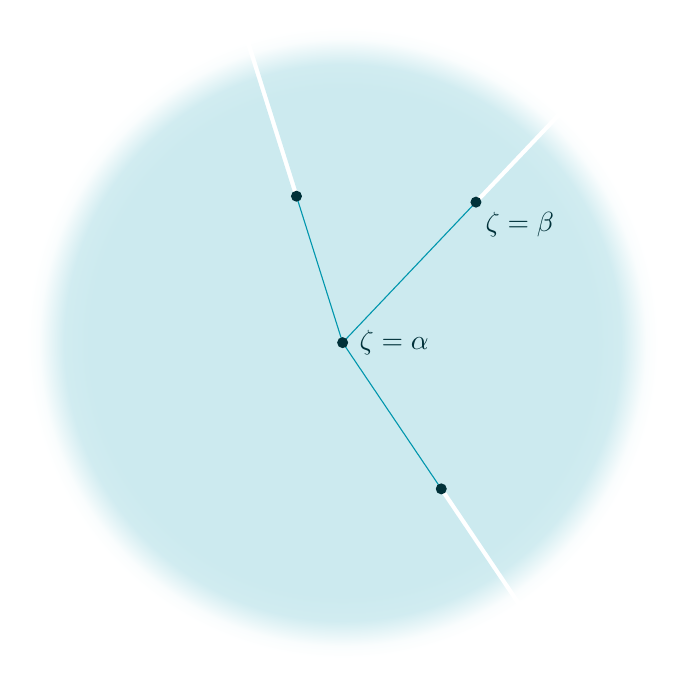
\begin{tikzpicture}
\newcommand{\spill}{4}
\newcommand{\slitsize}{0.4}
\fill[ietcoast!20, bezier bounding box, path fading=radial edge]
  (-\spill, -\spill) (\spill, \spill)
  (0, 0) -- (180:\spill)
  arc (180:107.5+\slitsize:\spill) -- (107.5+\spill/1.95*\slitsize:1.95) -- (107.5-\spill/1.95*\slitsize:1.95) -- (107.5-\slitsize:\spill)
  arc (107.5-\slitsize:46.5+\slitsize:\spill) -- (46.5+\spill/2.46*\slitsize:2.46) -- (46.5-\spill/2.46*\slitsize:2.46) -- (46.5-\slitsize:\spill)
  arc (46.5-\slitsize:-56+\slitsize:\spill) -- (-56+\spill/2.24*\slitsize:2.24) -- (-56-\spill/2.24*\slitsize:2.24) -- (-56-\slitsize:\spill)
  arc (-56-\slitsize:-180:\spill) -- (0, 0);
\node[ietcoast!33!black, anchor=north west] at (46.5:2.46) {$\zeta = \beta$};
\foreach \p in {(107.5:1.95), (46.5:2.46), (-56:2.24)} {
  \draw[ietcoast] \p -- (0,0);
  \fill[ietcoast!33!black] \p circle (0.7mm);
}
\fill[ietcoast!33!black] circle (0.7mm) node[anchor=180, outer sep=1mm] {$\zeta = \alpha$};
\end{tikzpicture}
\end{center}
\caption{The domain $\Omega_\alpha$}\label{Fig:slit domain}
\end{figure}
Let us calculate the jump of $\int_{\mathcal{C}_\alpha^\theta(\zeta)}\nu$ across the cut starting at $\zeta = \beta$. Write $\beta$ as $\alpha + re^{i\theta_\beta}$, and let $\beta^+$ and $\beta^-$ be the points we get by infinitesimally increasing or decreasing $\theta_\beta$. The jump is then given by \[\int_{\mathcal{C}_\alpha^\theta(\beta^+)} \nu - \int_{\mathcal{C}_\alpha^\theta(\beta^-)} \nu\] 
and it is 
which turns out to be proportional to $\tilde{\phi}_\beta$, namely to the germ of analytic functions at $\zeta_\alpha=\beta$. %We will see an example of this behaviour in Appendix~\ref{apx:eye-res-airy}. 


\textcolor{Navy}{Initially, the function $\int_{\mathcal{C}_j(\zeta)} \nu$ is only defined for $\zeta$ on the ray $[\alpha_j, \infty)$, but it can be analytically continued to points off the ray by homotopy of the path $\mathcal{C}_j(\zeta)$. Since $\nu$ is holomorphic, the only way for $\int_{\mathcal{C}_j(\zeta)} \nu$ to be singular is for something to go wrong with the hotmotopy of $\mathcal{C}_j(\zeta)$. At a critical point of $f$, the ends of the homotoped path $\mathcal{C}_j(\zeta)$ come together, telling us that.}
\end{remark}
\textcolor{orange}{
\begin{corollary}\label{simple-res-thimble}
    If $f$ and $\nu$ are polynomials, the function ${\phi}=\fracderiv{-1/2}{\zeta}{\alpha}\iota$ defined in Remark~\ref{rmk:1/2-deriv} has simple resurgent singularities at $\zeta=\beta$, for all $\beta$ roots of $P$ such that $\beta\neq\alpha$.  
\end{corollary}
\begin{proof}
    Recall ${\phi}_\alpha$ is the sum of the Borel transform of $z^{1/2}\tilde{I}_j$, namely 
    \[\hat{\phi}_j(\zeta)=\fracderiv{1/2}{\zeta}{\alpha_j}\hat{\iota}_j=\int_{\alpha_j}^\zeta(\zeta-s)^{-3/2}\hat{\iota}_j(s)\, ds\]
    Then by Pham's result (see \eqref{rmk:Pham formula}) we know 
    \[\hat{\iota}_j(\zeta_j)=\frac{(-\zeta_j)^{-1/2}}{2\pi i\Gamma(-\tfrac{1}{2})}\sum_{k=0}^\infty c_k (-\zeta_j)^{-k} + \text{ hol. funct. }\]
hence 
\[\hat{\iota}_j(\zeta)=\int_{\alpha_j}^\zeta(\zeta-s)^{-3/2}\frac{(-s+\alpha_j)^{-1/2}}{2\pi i\Gamma(-\tfrac{1}{2})}\sum_{k=0}^\infty c_k (-s+\alpha_j)^{-k} \, ds + \text{ hol. funct. }\]
\end{proof}
}
\begin{remark}\label{rmk:Pham formula}
    When $f$ and $\nu$ are polynomials and $X$ is $N$-dimensional, a result of Pham \cite[Equation 2.4, II partie]{pham} allows to write ${\iota}$ explicitly as 
    \begin{equation}\label{eqn:Pham}
        (-1)^{\frac{N(N-1)}{2}}  \sum_{k=0}^\infty c_k\, \delta^{-\frac{N}{2}-k}+ \text{ hol. funct.}
    \end{equation}
    for some coefficients $c_k$ which depends on $f$ and $\nu$, and with $\delta^{-\ell}$ be defined as
   \begin{equation*}
       \delta^{-\ell}:=\begin{cases}
           \frac{\zeta^{\ell-1}}{-2\pi i(\ell-1)!}\log(\zeta) + \text{ hol. funct.} & \text{ if } \ell\in\mathbb{N}^*\\
           & \\
           \frac{(-\zeta)^{\ell-1}}{2\pi i\, \Gamma(-\ell)}+ \text{ hol. funct.} & \text{ if } \ell\notin \mathbb{N}^* 
       \end{cases}
   \end{equation*}
In particular, if $N=1$, the inverse Laplace transform of $I$ has a fractional power singularity of order $1/2$ at the origin, as we compute explicitly in the proof of Theorem~\ref{thm:maxim-proof}. %as computed in Remark~\ref{rmk:1/2-deriv} the inverse Laplace tranform of $z^{-1/2} I$ is the $1/2$-derivative of ${\iota}$, hence it has \textcolor{orange}{simple singularities (see Corollary~\ref{simple-res-thimble})}. \textcolor{magenta}{We expect this result to hold beyond the polynomial case.} We also expect that equation \eqref{eqn:formula-proof} can be generalized to the $N$-dimensional case replacing the $1/2$-derivative with the $N/2$ one. 
\end{remark}
\section{Examples}\label{sec:examples}
%
\subsection{Airy}\label{sec:airy}
%
The Airy equation is
\begin{equation}\label{eqn:airy}
\left[\big(\tfrac{\partial}{\partial y}\big)^2 - y\right] \Phi = 0.
\end{equation}
One solution is given by the Airy function,
\[ \Ai(y) = \frac{1}{2\pi i} \int_\gamma \exp\left(\tfrac{1}{3}t^3 - yt\right)\,dt, \]
where $\gamma$ is a path that comes from $\infty$ at $-60^\circ$ and returns to $\infty$ at $60^\circ$. \textcolor{Pink}{[Figure~\ref{fig:path_Airy} shows integration contour after change of coordinates]}

With the substitution $t = 2uy^{1/2}$, we can rewrite the Airy integral as
\[ \Ai(y) = y^{1/2}\;\frac{1}{\pi i} \int_{\mathcal{C}^\theta_1} \exp\left[\tfrac{2}{3}y^{3/2} \left(4u^3 - 3u\right)\right]\,du, \]
where $\mathcal{C}^\theta_1$ is the contour that passes through the point $u = \tfrac{1}{2}$ and projects to the ray $\mathcal{J}^\theta_{\zeta, 1}$ under the mapping $-\zeta = 4u^3 - 3u$.
\begin{center}
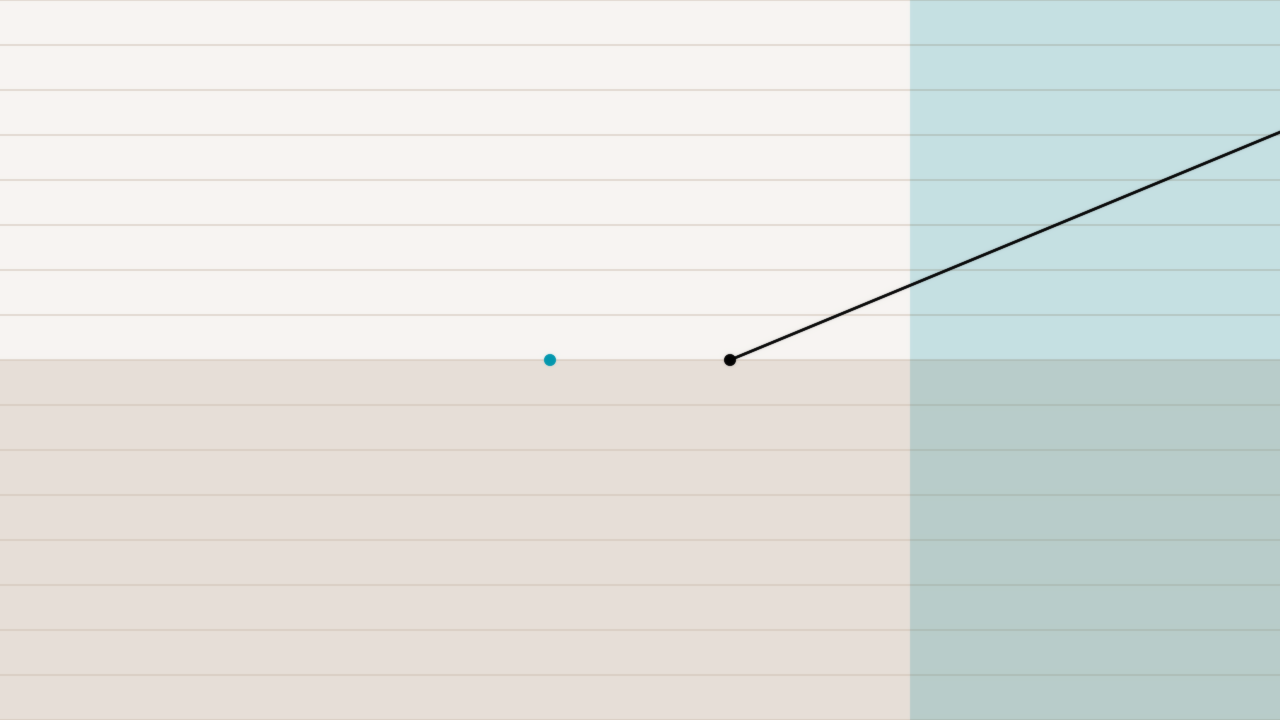
\includegraphics[width=6.5cm]{figures/ray_1_ge3.png}
\hspace{0.5cm}
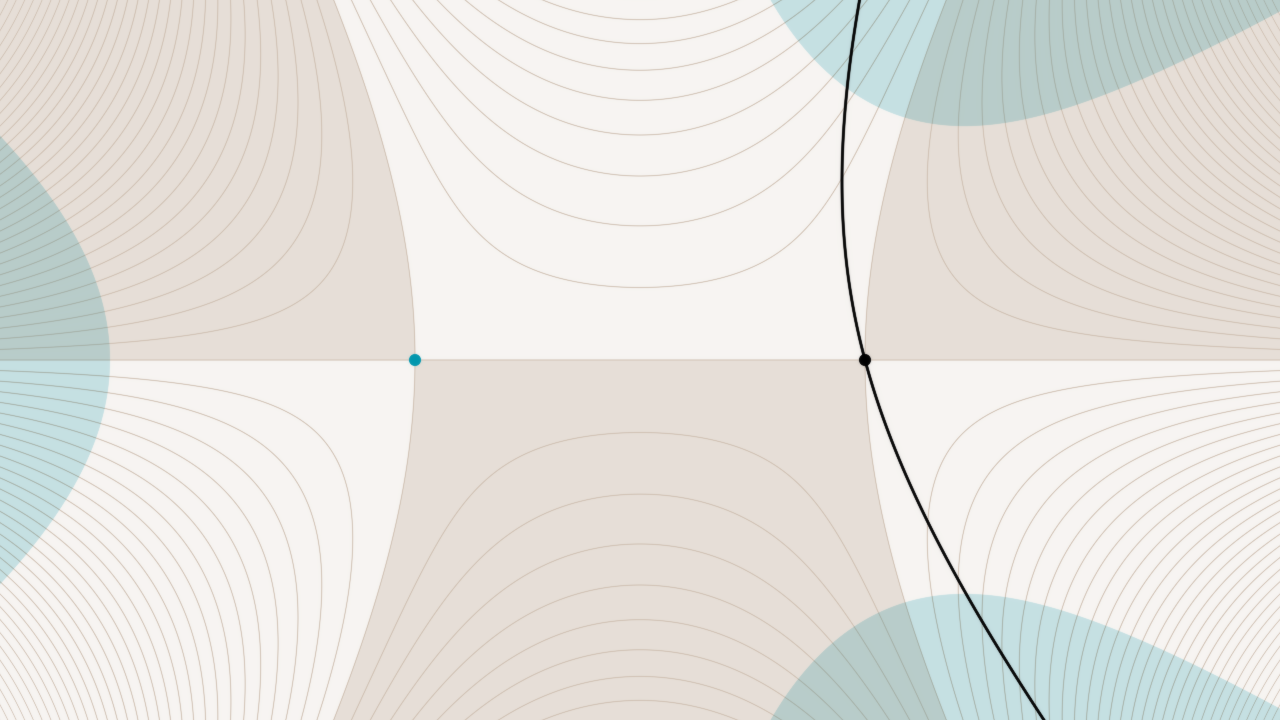
\includegraphics[width=6.5cm]{figures/thimble-n3_1.png}
\captionof{figure}{The ray $\mathcal{J}^{\pi/8}_{\zeta, 1}$ in the $\zeta$ plane and its preimage $\mathcal{C}^{\pi/8}_1$ in the $u$ plane. The upper and lower halves of the $\zeta$ plane are colored light and dark, so their preimages form a checker pattern on the $u$ plane. The region $\Re(\zeta) > 3$ and its preimage in the $u$ plane are shaded.}\label{fig:path_Airy}
\end{center}

Note that $4u^3 - 3u$ is the third Chebyshev polynomial. By considering other Chebyshev polynomials, we can situate the Airy function within the family of {\em Airy-Lucas functions}. Treating these functions as a family adds more insight than complexity, so we will go straight to the general case. However, since the Airy function is a classic example in the study of Borel summation and resurgence, it may be worth seeing on its own. In Appendix~\ref{airy-appendix}, we give a detailed treatment of the Airy function, specializing our arguments from the general case.

\subsection{Airy--Lucas}\label{example_AL}
The Airy-Lucas equation is
\begin{equation}\label{eqn:airy-lucas}
\left[\big(\tfrac{\partial}{\partial y}\big)^2 - (m-1) y^{-1} \tfrac{\partial}{\partial y} - y^{n-2}\right] \Phi = 0
\end{equation}
with $n \in \{3, 4, 5, \ldots\}$ and $m \in \{1, 2, \ldots, n-1\}$. A few solutions, indexed by $j \in \{1, \ldots, n-1\}$, are given by the Airy-Lucas functions~\cite[equation~3.6]{charbonnier22}
\[ \widehat{\Ai}^{(j)}_{n, m-1}(y) = \left\{\begin{array}{ll}i & j \text{ odd} \\ 1 & j \text{ even}\end{array}\right\} \frac{y^{m/2}}{\pi} \int_{\mathcal{C}^\theta_j} \exp\left[\tfrac{2}{n} y^{n/2}\,T_n(u)\right]\,U_{m-1}(u)\,du, \]
where $\mathcal{C}^\theta_j$ is the contour that passes through the point $u = \cos\big(\tfrac{j}{n}\pi\big)$ and projects to the ray $\mathcal{J}^\theta_{\zeta, \pm 1}$ under the mapping $-\zeta = T_n(u)$. \textcolor{RoyalBlue}{where $\mathcal{C}^\theta_j$ is the Lefschetz thimble through $u = \cos\big(\tfrac{j}{n}\pi\big)$. By definition, $\mathcal{C}^\theta_j$ is a preimage of the ray $\mathcal{J}^\theta_{\mp 1}$ under the function $-T_n(u)$.} The ray starts at the critical value $1$ when $j$ is odd, and $-1$ when $j$ is even.
\begin{center}
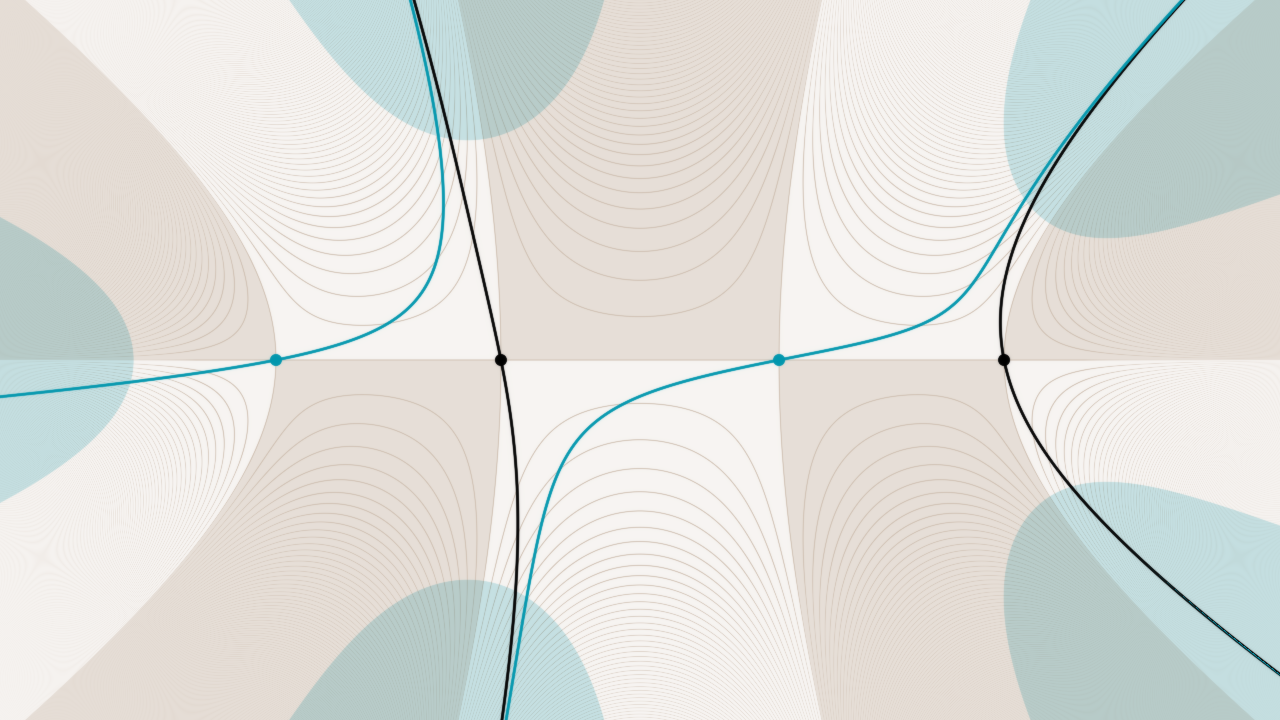
\includegraphics[width=10cm]{figures/thimbles-n5.png}
\captionof{figure}{The integration contours $\mathcal{C}^{\pi/8}_1, \ldots, \mathcal{C}^{\pi/8}_4$ for the Airy--Lucas functions with $n=5$. The dark and light thimbles are the preimages of the rays $\mathcal{J}^{\pi/8}_{\zeta, 1}$ and $\mathcal{J}^{\pi/8}_{\zeta, -1}$, respectively.}\label{fig:thimble_n_5}
\end{center}
\subsubsection{Rewriting as a modified Bessel $\frac{m}{n}$ equation}
We can distill the most interesting parts of the Airy-Lucas function by writing
\[ \widehat{\Ai}^{(j)}_{n, m-1}(y) = \frac{2 \sinh\big(\tfrac{m}{n}\,i\pi\big)}{n\pi} \left\{\begin{array}{ll}i & j \text{ odd} \\ 1 & j \text{ even}\end{array}\right\}\,y^{{m/2}}\,K^{(j)}_{m/n}\big(\tfrac{2}{n} y^{n/2}\big), \]
where
\begin{equation}\label{integral:mod-bessel-rational-AL}
K^{(j)}_{m/n}(z) = \frac{n}{2 \sinh\big(\tfrac{m}{n}\,i\pi\big)}\int_{\mathcal{C}^\theta_j} \exp\left[z T_n(u)\right]\,U_{m-1}(u)\,du.
\end{equation}
Saying that $\widehat{\Ai}^{(j)}_{n, m-1}$ satisfies the Airy-Lucas equation is equivalent to saying that $K^{(j)}_{m/n}$ satisfies the modified Bessel equation with parameter $\frac{m}{n}$:
\begin{equation}\label{eqn:mod-bessel-AL}
\left[z^2 \big(\tfrac{\partial}{\partial z}\big)^2 + z \tfrac{\partial}{\partial z} - \big[\big(\tfrac{m}{n} \big)^2 + z^2\big]\right] \Phi = 0.
\end{equation}
%%[DROPPED] In fact, as we will see in Section~\ref{contour-argument-AL}, $K$ is the modified Bessel function $K_{{m/n}}$.
Let us put equation~\eqref{eqn:mod-bessel-AL} in the form $\mathcal{P}\Phi=0$ with $\mathcal{P}$ as in equation~\eqref{eqn:operator-P}:
\begin{equation}\label{eqn:reg-mod-bessel-AL}
\left[ \big[ \big(\tfrac{\partial}{\partial z}\big)^2 - 1 \big] + z^{-1} \tfrac{\partial}{\partial z} - \big({\tfrac{m}{n}}\big)^2 z^{-2} \right] \Phi = 0.
\end{equation}

\subsubsection{Asymptotic analysis}\label{sec:asympt-AL}
From the work of Poincar\'{e} and the Ramis Index Theorem, as discussed at the beginning of Section~\ref{sec:new-summability-proof}, we know that equation~\eqref{eqn:reg-mod-bessel-AL} has a frame of formal $1$-Gevrey trans-monomial solutions
\[ \{ e^{-\alpha z} z^{-\tau_\alpha}\,\series{W}_\alpha \mid \alpha^2 - 1 = 0 \}, \]
where $\tau_\alpha = 1/2$ and $\series{W}_\alpha\in\C\llbracket z^{-1} \rrbracket_1$. From \cite[Equations 10.40.2 and 10.17.1]{dlmf}, we learn that $K_{m/n}(z) \sim \left(\tfrac{\pi}{2}\right)^{1/2} e^{-z} z^{-1/2}\,\series{W}_1$, with
\begin{equation}\label{bessel-asymp-AL}
\series{W}_1 = 1 - \frac{\left(\tfrac{1}{2}-\tfrac{m}{n}\right)_1 \left(\tfrac{1}{2}+\frac{m}{n}\right)_1}{2^1 \cdot 1!}\;z^{-1} + \frac{\left(\tfrac{1}{2}-\tfrac{m}{n}\right)_2 \left(\tfrac{1}{2}+\tfrac{m}{n}\right)_2}{2^2 \cdot 2!}\;z^{-2} - \frac{\left(\tfrac{1}{2}+\tfrac{m}{n}\right)_3 \left(\tfrac{1}{2}+\tfrac{m}{n}\right)_3}{2^3 \cdot 3!}\;z^{-3} + \ldots
\end{equation}

The holomorphic analysis in Section~\ref{big-idea} will give us holomorphic solutions
\[ \{ e^{-\alpha z} z^{-\tau_\alpha}\,W_\alpha \mid \alpha^2 - 1 = 0 \}, \]
which seem analogous to the trans-monomials above. Borel summation makes the analogy precise. We will see in Section~\ref{bessel-regularity-AL} that each $z^{-\tau_\alpha}\,W_\alpha$ is proportional to the Borel sum of $z^{-\tau_\alpha}\,\series{W}_\alpha$, as required by Theorem~\ref{thm:summability_ODE}.
%\subsection{Going to the spatial domain}\label{spatial-AL}
\subsubsection{The big idea}\label{big-idea}
We are going to look for functions $v_\alpha$ whose Laplace transforms $\laplace_{\zeta, \alpha} v_\alpha$ satisfy equation~\eqref{eqn:reg-mod-bessel-AL}. We will succeed when $\alpha^2 - 1 = 0$, and we will see that $K_{m/n}$ is a scalar multiple of $\laplace_{\zeta, 1} v_1$.

By the properties of the Laplace transform laid out in Proposition~\ref{prop:L-int-op}, a function $\laplace_{\zeta, \alpha} v$ satisfies the differential equation~\eqref{eqn:reg-mod-bessel-AL} if and only if $v$ satisfies the integral equation
\begin{equation}\label{int-eq:spatial-mod-bessel-AL}
\left[ \big[ \zeta^2 - 1 \big] - \fracderiv{-1}{\zeta}{\alpha} \circ \zeta - \big(\tfrac{m}{n}\big)^2 \fracderiv{-2}{\zeta}{\alpha} \right] v = 0.
\end{equation}
It is tempting to differentiate both sides of this equation until we get
\begin{equation}\label{diff-eq:spatial-mod-bessel-AL}
\left[ \big(\tfrac{\partial}{\partial \zeta}\big)^2 \circ \big[ \zeta^2 - 1 \big] - \tfrac{\partial}{\partial \zeta} \circ \zeta - \big(\tfrac{m}{n}\big)^2 \right] v = 0,
\end{equation}
which is easier to solve. Unfortunately, a solution of equation~\eqref{diff-eq:spatial-mod-bessel-AL} will not satisfy equation~\eqref{int-eq:spatial-mod-bessel-AL} in general. However, as we show in Appendix~\ref{shifting}, a solution of equation~\eqref{diff-eq:spatial-mod-bessel-AL} {\em will} satisfy equation~\eqref{int-eq:spatial-mod-bessel-AL} if it belongs to $(\zeta - \alpha)^\sigma \mathcal{O}_{\zeta = \alpha}$ for some $\sigma \in (-1, 0)$.

This is good news, because equation~\eqref{diff-eq:spatial-mod-bessel-AL} has a regular singularity at each root of $\zeta^2 - 1$, and the Frobenius method often gives a solution of the desired kind at each regular singular point. We can see the regular singularities by moving the derivatives to the right:
\[ \left[ (\zeta^2 - 1) \big(\tfrac{\partial}{\partial \zeta}\big)^2 + 3\zeta \tfrac{\partial}{\partial \zeta} + \big[ 1 - \big(\tfrac{m}{n}\big)^2 \big] \right] v = 0. \]

In Sections \ref{pos-root-AL}\,--\,\ref{neg-root-AL}, we will see this approach succeed. For each root $\alpha$, we will find a solution $v_\alpha$ of equation~\eqref{diff-eq:spatial-mod-bessel-AL} that belongs to $(\zeta - \alpha)^{\tau_\alpha-1}\,\mathcal{O}_{\zeta = \alpha}$ for some constant $\tau_\alpha \in (0, 1)$. We will express $v_\alpha$ explicitly enough to see that it extends to a function in $\singexpalg{\tau_\alpha-1}(\Omega_\alpha)$ on any sector $\Omega_\alpha$ that has its tip at $\zeta = \alpha$ and does not touch the other root.
\textcolor{LimeGreen}{Furthermore, we will show in Section~\ref{bessel-regularity-AL} that $v_\alpha$ can be analytically continued to a function in $\singexpalg{\tau_\alpha-1}(\Omega_\alpha)$, where $\Omega_\alpha$ is a sector with its tip at $\zeta = \alpha$.}
%%and can be analytically continued to a sector $\Omega_\alpha$ with its tip at $\zeta = \alpha$. In fact $v_\alpha$ will belong to $\zeta_\alpha^{\tau_\alpha-1}\,\mathcal{O}_{\zeta=\alpha} \cap$
%%which is in $\singexpalg{\tau_\alpha-1}(\Omega_\alpha)$ for some constant $\tau_\alpha \in (0, 1)$ and some domain $\Omega_\alpha$ resembling the one in the figure from Theorem~\ref{re:thm:exist_uniq_ODE}.
It follows by Proposition~\ref{prop:laplace-cont} that for any ray $\mathcal{J}^\theta_{\zeta, \alpha}$ in $\Omega_\alpha$, the Laplace transform $\laplace^\theta_{\zeta, \alpha} v_\alpha$ is a well-defined element of $\dualsingexp{-\tau_\alpha}{\Lambda}(\widehat{\Omega}_\alpha^\Lambda)$ that satisfies equation~\eqref{eqn:reg-mod-bessel-AL}. Using the technique from the proof of Lemma~\ref{lem:laplace-bridge}, we can see more precisely that $\laplace^\theta_{\zeta, \alpha} v_\alpha$ belongs to
\[ cz^{-\tau_\alpha} + \dualsingexp{-\tau_\alpha-1}{\Lambda}(\widehat{\Omega}_\alpha^\Lambda) \]
for some non-zero constant $c$, confirming the existence part of Theorem~\ref{re:thm:exist_uniq_ODE}.

We know from Section~\ref{sec:change-translation} that
\[ \laplace^\theta_{\zeta, \alpha} v_\alpha = e^{-\alpha z} V_\alpha \]
for $V_\alpha \defeq \laplace^\theta_{\zeta_\alpha, 0} v_\alpha$ and $\zeta = \alpha + \zeta_\alpha$. Observing that multiplication by $z^{-\tau_\alpha}$ gives an isometry $\dualsingexp{0}{\Lambda}(\widehat{\Omega}_\alpha^\Lambda) \to \dualsingexp{-\tau_\alpha}{\Lambda}(\widehat{\Omega}_\alpha^\Lambda)$, we can do the further decomposition
\[ \laplace_{\zeta, \alpha} v_\alpha = e^{-\alpha z} z^{-\tau_\alpha} W_\alpha, \]
where $W_\alpha$ is a bounded holomorphic function on $\widehat{\Omega}_\alpha^\Lambda$.

\textcolor{LimeGreen}{We can see from Section~\ref{sec:reg-decay} that $V_\alpha$ is asymptotic to a scalar multiple of $z^{-1 - \tau_\alpha}$ at $z = \infty$, so the further decomposition
\[ \laplace_{\zeta, \alpha} v_\alpha = e^{-\alpha z} z^{-\tau_\alpha} W_\alpha, \]
makes $W_\alpha$ asymptotic to a scalar multiple of \textcolor{magenta}{$z^{-1}$} at $z = \infty$.}
%\color{Peru}
%\begin{align*}
%\left[ \big(\tfrac{\partial}{\partial \zeta}\big)^2 \circ (\zeta - 1)(\zeta + 1) - \tfrac{\partial}{\partial \zeta} \circ \zeta - \big(\tfrac{1}{3}\big)^2 \right] v & = 0
%\end{align*}
%\color{Sienna}
%\begin{align*}
%\left[ \big[ 2 + 2(2\zeta) \tfrac{\partial}{\partial \zeta} + (\zeta^2 - 1) \big(\tfrac{\partial}{\partial \zeta}\big)^2 \big] - \big[ 1 + \zeta \tfrac{\partial}{\partial \zeta} \big] - \big(\tfrac{1}{3}\big)^2 \right] v & = 0 \\
%\left[ (\zeta^2 - 1) \big(\tfrac{\partial}{\partial \zeta}\big)^2 + 3\zeta \tfrac{\partial}{\partial \zeta} + \big[ 1 - \big(\tfrac{1}{3}\big)^2 \big] \right] v & = 0 \\
%\left[ (\zeta - 1)(\zeta + 1) \big(\tfrac{\partial}{\partial \zeta}\big)^2 + 3\zeta \tfrac{\partial}{\partial \zeta} + \big[ 1 - \big(\tfrac{1}{3}\big)^2 \big] \right] v & = 0
%\end{align*}
%\color{black}
%%In terms of the coordinate $\zeta_\alpha$ with $\zeta = \alpha + \zeta_\alpha$, this equation is written
%%\begin{equation}\label{eqn:centered-mod-bessel}
%%\[ \left[ \big[ \zeta_\alpha (\zeta_\alpha + 2\alpha) + \alpha^2 - 1 \big] + \fracderiv{-1}{\zeta_\alpha}{0} \circ \big[ \zeta_\alpha + \alpha \big] - \big(\tfrac{1}{3}\big)^2 \fracderiv{-2}{\zeta_\alpha}{0} \right] w = 0. \]
%%\end{equation}
\subsubsection{Focus on $\zeta = 1$}\label{pos-root-AL}
Let us find a germ in $(\zeta-1)^{\tau_1-1}\,\mathcal{O}_{\zeta=1}$, for some $\tau_1 \in (0, 1)$, that satisfies equation~\eqref{diff-eq:spatial-mod-bessel-AL}. Define a new coordinate $\zeta_1$ on $\C$ so that $\zeta = 1 + \zeta_1$. In this coordinate, equation~\eqref{diff-eq:spatial-mod-bessel-AL} looks like
\begin{equation}\label{diff-eq:spatial-mod-bessel-pos-AL}
\left[\zeta_1(2 + \zeta_1) \big(\tfrac{\partial}{\partial \zeta_1}\big)^2 + 3(1 + \zeta_1) \tfrac{\partial}{\partial \zeta_1} + \big[1 - \big(\tfrac{m}{n}\big)^2\big]\right] v = 0.
\end{equation}
With another change of coordinate, given by $\zeta_1 = -2\xi_1$, we can rewrite equation~\eqref{diff-eq:spatial-mod-bessel-AL} as the hypergeometric equation
\begin{equation}\label{diff-eq:hypergeom-pos-AL}
\left[\xi_1 (1 - \xi_1) \big(\tfrac{\partial}{\partial \xi_1}\big)^2 + 3(\tfrac{1}{2} - \xi_1) \tfrac{\partial}{\partial \xi_1} - \big[1 - \big(\tfrac{m}{n}\big)^2\big]\right] v = 0.
\end{equation}
Looking through the twenty-four expressions for Kummer's six solutions, we find one \cite[formula~15.10.12]{dlmf} that represents a germ in $\xi_1^{-1/2}\,\mathcal{O}_{\xi_1=0}$:
\begin{alignat*}{2}
v_1 &=\;& \hphantom{-i\sqrt{2}}\,\xi_1^{-1/2} & {}_2F_1\big(\tfrac{1}{2}-\tfrac{m}{n}, \tfrac{1}{2}+\tfrac{m}{n}; \tfrac{1}{2}; \xi_1\big) \\[1mm]
&=\;& -i\sqrt{2}\,\zeta_1^{-1/2} & {}_2F_1\big(\tfrac{1}{2}-\tfrac{m}{n}, \tfrac{1}{2}+\tfrac{m}{n}; \tfrac{1}{2}; -\tfrac{1}{2}\zeta_1\big)
\end{alignat*}
From the argument in Section~\ref{big-idea} \textcolor{magenta}{(!)}, we know that $\laplace^\theta_{\zeta, 1} v_1$ is well-defined, satisfies equation~\eqref{eqn:mod-bessel-AL}, and can be written as $e^{-z} V_1$, where $V_1 = \laplace_{\zeta_1, 0} v_1$. Since $v_1$ \textcolor{magenta}{has order $-1/2$}, the decomposition $V_1 = z^{-1/2} W_1$ makes $W_1$ asymptotic to a scalar multiple of $1+O(z^{-1})$ at $z = \infty$.
\subsubsection{Focus on $\zeta = -1$}\label{neg-root-AL}
Let us find a germ in $(\zeta+1)^{\tau_{-1}-1}\,\mathcal{O}_{\zeta=-1}$, for some $\tau_{-1} \in (0, 1)$, that satisfies equation~\eqref{diff-eq:spatial-mod-bessel-AL}. In the rescaled coordinate from Section~\ref{pos-root-AL}, this is the point $\xi_1 = 1$. Looking again through Kummer's table of solutions, we find another expression \cite[formula~15.10.14]{dlmf} that represents a germ in $(1-\xi_1)^{-1/2}\,\mathcal{O}_{\xi_1=1}$:
\begin{alignat*}{2}
v_{-1} &=\;& (1-\xi_1)^{-1/2} &\;{}_2F_1\big(\tfrac{1}{2}-\tfrac{m}{n}, \tfrac{1}{2}+\tfrac{m}{n}; \tfrac{1}{2}; 1-\xi_1\big) \\[1mm]
&=\;& \sqrt{2}\,\zeta_{-1}^{-1/2} &\;{}_2F_1\big(\tfrac{1}{2}-\tfrac{m}{n}, \tfrac{1}{2}+\tfrac{m}{n}; \tfrac{1}{2}; \tfrac{1}{2}\zeta_{-1}\big)
\end{alignat*}
where $\zeta_{-1}$ is the coordinate with $\zeta = -1 + \zeta_{-1}$. From the argument in Section~\ref{big-idea}, we know that $\laplace_{\zeta, -1} v_{-1}$ satisfies equation~\eqref{eqn:mod-bessel-AL}, and can be written as $e^z V_{-1}$, where $V_{-1} = \laplace_{\zeta_{-1}, 0} v_{-1}$. Since $v_{-1}$, like our other solution, \textcolor{magenta}{has order $-1/2$}, the same decomposition $V_{-1} = z^{-1/2} W_{-1}$ makes $W_{-1}$ asymptotic to a scalar multiple of $1+O(z^{-1})$ at $z = \infty$.

In this example, $v_1$ and $v_{-1}$ happen to be related by a symmetry: the M\"{o}bius transformation that pulls $\zeta$ back to $-\zeta$. Kummer's solutions typically come from six different hypergeometric equations, which are related by the M\"{o}bius transformations that permute their singularities. In our case, though, exchanging $1$ with $-1$ keeps equation~\eqref{diff-eq:spatial-mod-bessel-AL} the same.
\subsubsection{Abstract argument for Borel regularity}\label{bessel-regularity-AL}
The analysis in Sections~\ref{big-idea}--\ref{neg-root-AL} picks out a frame in the space of analytic solutions of~\eqref{eqn:reg-mod-bessel-AL}. The frame is generated by solutions of the form $\laplace_{\zeta, 1} v_1$ and $\laplace_{\zeta, -1} v_{-1}$, with $v_\alpha \in \singexpalg{-1/2}(\Omega_\alpha)$.
\begin{verify}
We get $v_\alpha$ from the existence result in Section~\ref{borel_reg-ODE}, which gives $v_\alpha = \zeta^{\tau_\alpha-1} + v_\alpha'$ with $\tau \in (0, \infty)$ and $v_j' \in \holoL{\infty, 1-\tau-\epsilon}(\Omega)$ \textcolor{magenta}{[What is this space? does not match notation from {\tt reg-sing-volterra}]} for some $\epsilon \in (0, 1]$. Looking back at the definitions of our weighted $L^\infty$ spaces, we can see that
\begin{align*}
v_j' \in \holoL{\infty, 1-\tau-\epsilon}(\Omega) & \Longrightarrow \zeta_j^{1-\tau-\epsilon}\,v_j' \text{ is bounded near } \zeta_j = 0 \\
& \Longrightarrow \zeta_j^\epsilon\,\zeta_\alpha^{1-\tau-\epsilon}\,v_j' \text{ goes to } 0 \text{ as } \zeta_\alpha \text{ goes to } 0 \\
& \Longrightarrow \zeta_\alpha^{1-\tau}\,v_\alpha' \text{ goes to } 0 \text{ as } \zeta_\alpha \text{ goes to } 0 \\
& \Longrightarrow v_\alpha' / \zeta_\alpha^{\tau_\alpha-1} \text{ goes to } 0 \text{ as } \zeta_\alpha \text{ goes to } 0 \\
& \Longleftrightarrow v_j' \in o\big(\zeta_\alpha^{\tau_\alpha-1}\big).
\end{align*}
In this case, $\tau_\alpha = \tfrac{1}{2}$.
\end{verify}

The Poincar\'{e} algorithm, as we saw in Section~\ref{sec:asympt-AL}, picks out a frame in the space of formal trans-series solutions of equation~\eqref{eqn:reg-mod-bessel-AL}. The frame is generated by trans-monomial solutions of the form $e^{-z} z^{-1/2}\,\tilde{W}_1$ and $e^z z^{-1/2}\,\tilde{W}_{-1}$, with $\tilde{W}_j \in \C\llbracket z^{-1} \rrbracket$. We will now show that if these solutions are Borel-summable, their Borel sums generate the same frame as $\laplace_{\zeta, 1} v_1$ and $\laplace_{\zeta, -1} v_{-1}$. \textcolor{orange}{[We're following the version of the argument that shows the Poincar\'{e} solutions exist and are 1-Gevrey.]}

The Borel transform maps $e^{-\alpha z} z^{-1/2}\,\C\llbracket z^{-1} \rrbracket$ into $\zeta_\alpha^{-1/2}\,\C\llbracket \zeta_j \rrbracket$ \textcolor{magenta}{(see Section \ref{sec:action_transseries})}, and it turns formal trans-monomial solutions of equation~\eqref{eqn:reg-mod-bessel-AL} into formal power series solutions of equation~\eqref{int-eq:spatial-mod-bessel-AL}. Summation sends convergent power series in $\zeta_\alpha^{-1/2}\,\C\llbracket \zeta_\alpha \rrbracket$ into $\zeta_\alpha^{-1/2}+ o\big(\zeta_\alpha^{-1/2}\big)$ \textcolor{orange}{[since the argument above is one-way, is not this weaker than being in $\singexpalg{-1/2}$?]}, and it turns convergent power series that satisfy a given fractional integral equation into holomorphic functions that satisfy the same equation \cite[Lemma 2]{reg-sing-volterra}. Thus, if $e^{-z} z^{-1/2}\,\tilde{W}_1$ and $e^z z^{-1/2}\,\tilde{W}_{-1}$ are $1$-Gevrey, their Borel transforms sum to solutions of equation~\eqref{int-eq:spatial-mod-bessel-AL}, which lie in $\singexpalg{-1/2}$ \textcolor{magenta}{[needs domain]} for $\alpha = 1$ and $\alpha = -1$, respectively.

When $\alpha$ is $1$ or $-1$, equation~\eqref{int-eq:spatial-mod-bessel-AL} becomes the kind of singular integral equation discussed in Section~\ref{borel_reg-ODE}. It therefore has exactly one solution in $\singexpalg{1/2}$ \textcolor{orange}{[needs domain]}, up to scaling. That means $\borel\big[ e^{-\alpha z} z^{-1/2}\,\tilde{W}_\alpha \big]$ must sum to a scalar multiple of $v_\alpha$. Thus, if $e^{-\alpha z} z^{-1/2}\,\tilde{W}_\alpha$ is Borel-summable, its Borel sum is a scalar multiple of $\laplace_{\zeta, \alpha} v_\alpha$.

\subsubsection{Confirmation of Borel regularity}\label{confirmation-borel-regularity}
We can confirm the conclusion of Section~\ref{bessel-regularity-AL} using our explicit expressions for the formal power series $\tilde{W}_\alpha$ and the functions $v_\alpha$. We found in Section~\ref{sec:asympt-AL} that
\begin{align*}
\tilde{W}_1 & = \sum_{k = 0}^{\infty} \frac{\left(\tfrac{1}{2}-\tfrac{m}{n}\right)_k \left(\tfrac{1}{2}+\tfrac{m}{n}\right)_k}{k!} \left(-\frac{1}{2}\right)^k z^{-k} \\
\tilde{W}_{-1} & = \sum_{k = 0}^{\infty} \frac{\left(\tfrac{1}{2}-\tfrac{m}{n}\right)_k \left(\tfrac{1}{2}+\tfrac{m}{n}\right)_k}{k!} \left(\frac{1}{2}\right)^k z^{-k}.
\end{align*}
Computing
\begin{align*}
\borel_\zeta \big[ e^{-z} z^{-1/2}\,\tilde{W}_1 \big] & = \borel_\zeta \left[ e^{-z} \sum_{k = 0}^{\infty} \frac{\left(\tfrac{1}{2}-\tfrac{m}{n}\right)_k \left(\tfrac{1}{2}+\tfrac{m}{n}\right)_k}{k!} \left(-\frac{1}{2}\right)^k z^{-k-\frac{1}{2}} \right] \\
& = \sum_{k = 0}^{\infty} \frac{\left(\tfrac{1}{2}-\tfrac{m}{n}\right)_k \left(\tfrac{1}{2}+\tfrac{m}{n}\right)_k}{k!} \left(-\frac{1}{2}\right)^k \frac{\zeta_1^{k-\frac{1}{2}}}{\Gamma\big(k+\frac{1}{2}\big)} \\
& = \sum_{k = 0}^{\infty} \frac{\left(\tfrac{1}{2}-\tfrac{m}{n}\right)_k \left(\tfrac{1}{2}+\tfrac{m}{n}\right)_k}{k!} \left(-\frac{1}{2}\right)^k \frac{\zeta_1^{k-\frac{1}{2}}}{\Gamma\big(\frac{1}{2}\big) \left(\frac{1}{2}\right)_k} \\
& = \frac{\zeta_1^{-\frac{1}{2}}}{\Gamma\big(\frac{1}{2}\big)} \sum_{k = 0}^{\infty} \frac{\left(\tfrac{1}{2}-\tfrac{m}{n}\right)_k \left(\tfrac{1}{2}+\tfrac{m}{n}\right)_k}{\left(\frac{1}{2}\right)_k} \left(-\frac{1}{2}\right)^k \frac{\zeta_1^k}{k!},
\end{align*}
we see that $\borel\big[ e^{-z} z^{-1/2}\,\tilde{W}_1 \big]$ sums to
\[ \tfrac{1}{\Gamma(1/2)}\,\zeta_1^{-1/2}\,{}_2F_1\big(\tfrac{1}{2}-\tfrac{m}{n}, \tfrac{1}{2}+\tfrac{m}{n}; \tfrac{1}{2}; -\tfrac{1}{2}\zeta_1\big). \]
Looking back at Section~\ref{pos-root-AL}, we recognize this as a scalar multiple of $v_1$. In fact, with the thimble projection reasoning, there is no ambiguity in the choice of the multiplicative constant. 


Through a similar calculation, we see that $\borel\big[ e^z z^{-1/2}\,\tilde{W}_{-1} \big]$ sums to
\[ \tfrac{1}{\Gamma(1/2)}\,\zeta_{-1}^{-1/2}\,{}_2F_1\big(\tfrac{1}{2}-\tfrac{m}{n}, \tfrac{1}{2}+\tfrac{m}{n}; \tfrac{1}{2}; \tfrac{1}{2}\zeta_{-1}\big). \]
Looking back at Section~\ref{neg-root-AL}, we recognize this as a scalar multiple of $v_{-1}$.



\subsubsection{Thimble projection reasoning for Airy-Lucas functions}\label{contour-argument-AL}
We follow the reasoning of the proof of Lemma~\ref{lem:thimble_proj_formula-proof}. We can recast integral~\eqref{integral:mod-bessel-rational-AL} into the $\zeta$ plane by setting $-\zeta = T_n(u)$, which implies that $-d\zeta = n U_{n-1}(u)\,du$. The critical point $u = \cos\big(\tfrac{j}{n}\pi\big)$ splits $\mathcal{C}^\theta_j$ into two pieces: the {\em incoming} branch, where the orientation of the thimble runs toward the critical point, and the {\em outgoing} branch, where the orientation points away. Recalling that $\mathcal{C}^\theta_j$ is a preimage of $\mathcal{J}^\theta_{\zeta, \mp 1}$, we get \textcolor{magenta}{[mention that $\theta$ should be $\arg z$]}
\begin{align*}%%\label{integral:mod-bessel-rational-zeta}
K^{(j)}_{m/n}(z) & = \frac{n}{2 \sinh\big(\tfrac{m}{n}\,i\pi\big)} \int_{\mathcal{C}^\theta_j} \exp\left[z T_n(u)\right]\,U_{m-1}(u)\,du \\
& = -\frac{1}{2\sinh\big(\tfrac{m}{n}\,i\pi\big)} \left[ \int_{\mathcal{J}^\theta_{\zeta, \mp 1}} e^{-z\zeta}\,\frac{U_{m-1}(u_+)}{U_{n-1}(u_+)}\,d\zeta - \int_{\mathcal{J}^\theta_{\zeta, \mp 1}} e^{-z\zeta}\,\frac{U_{m-1}(u_-)}{U_{n-1}(u_-)}\,d\zeta \right]
\end{align*}
where $u_-$ and $u_+$ are the lifts to the incoming and outgoing branches of $\mathcal{C}^\theta_j$, respectively. \begin{todo}[Draw the thimble in the $u$ plane?]\end{todo}

\color{NavyBlue}
Since the Chebyshev polynomial $T_n$ is defined by the identity $T_n(\cos(\phi)) = \cos(n\phi)$, we introduce a new variable $\phi$ with $u = \cos(\phi)$ and $-\zeta = \cos(n\phi)$. On the $\phi$ plane, which is an infinite branched cover of the $u$ plane, we can lift $\mathcal{C}^\theta_j$ to the path $\tfrac{j}{n}\pi + i\R$. The incoming and outgoing branches lift to $\tfrac{j}{n}\pi - i[0, \infty)$ and $\tfrac{j}{n}\pi + i[0, \infty)$, respectively. \begin{todo}[Draw the lifted thimble in the $\phi$ plane?]\end{todo}

We can now use identity~15.4.16 from \cite{dlmf} to write the integrand explicitly in terms of $\zeta$:
\begin{align*}
\frac{U_{m-1}(\cos(\phi))}{U_{n-1}(\cos(\phi))} &= \frac{\sin(m\phi)}{\sin(\phi)}\frac{\sin(\phi)}{\sin(n \phi)}\\
& = \frac{\sin(m\phi)}{\sin(n \phi)}\\
& = \frac{m}{n}\;{}_2F_1\left(\frac{1}{2} - \frac{m}{2n},\;\frac{1}{2} + \frac{m}{2n};\;\frac{3}{2};\;\sin^2(n \phi)\right) \\
& = \frac{m}{n}\;{}_2F_1\left(\frac{1}{2} - \frac{m}{2n},\;\frac{1}{2} + \frac{m}{2n};\;\frac{3}{2};\;1 - \zeta^2\right).
\end{align*}
Initially, we only know that this equation holds in the disk $|\phi| < \tfrac{\pi}{2n}$. However, observing that the left-hand side is meromorphic throughout the $\phi$ plane, we can deduce by analytic continuation that the equation holds throughout the $\phi$ plane.

Next, we simplify the integrand using identities 15.8.4 and 15.8.27--28 from \cite{dlmf}, which tell us that\begin{align*}
&{}_2F_1\left(\frac{1}{2} - \frac{m}{2n}, \frac{1}{2} + \frac{m}{2n}; \frac{3}{2}; 1 - \zeta^2\right) \\[3mm]
& =\; \hphantom{+} \frac{\pi}{\Gamma\left(1-\frac{m}{2n}\right) \Gamma\left(1 + \frac{m}{2n}\right)}\;{}_2F_1\left(\frac{1}{2} - \frac{m}{2n},\;\frac{1}{2} + \frac{m}{2n};\;\frac{1}{2};\;\zeta^2\right) \\
& \hphantom{=}\; - \frac{\pi \zeta}{\Gamma\left(\frac{1}{2} - \frac{m}{2n}\right) \Gamma\left(\frac{1}{2} + \frac{m}{2n}\right)}\;{}_2F_1\left(1 - \frac{m}{2n},\;1 + \frac{m}{2n};\;\frac{3}{2};\;\zeta^2\right) \\[3mm]
& =\; \hphantom{+ \frac{0}{0}}\;{}_2F_1\left(1 - \frac{m}{n},\;1 + \frac{m}{n};\;\frac{3}{2};\;\frac{1}{2} - \frac{\zeta}{2}\right) + \hphantom{\frac{0}{0}}\;{}_2F_1\left(1-\frac{m}{n},\;1 + \frac{m}{n};\;\frac{3}{2};\;\frac{1}{2} + \frac{\zeta}{2}\right) \\
& \hphantom{=}\; + \frac{1}{2}\;{}_2F_1\left(1-\frac{m}{n},\;1+\frac{m}{n};\;\frac{3}{2};\;\frac{1}{2} - \frac{\zeta}{2}\right) - \frac{1}{2}\;{}_2F_1\left(1-\frac{m}{n},\;1 + \frac{m}{n};\;\frac{3}{2};\;\frac{1}{2} + \frac{\zeta}{2}\right) \\[3mm]
& =\; \hphantom{+} \frac{3}{2}\;{}_2F_1\left(1 - \frac{m}{n},\;1 + \frac{m}{n};\;\frac{3}{2};\frac{1}{2} - \frac{\zeta}{2}\right) + \frac{1}{2}\;{}_2F_1\left(1 - \frac{m}{n},\;1 + \frac{m}{n};\;\frac{3}{2};\;\frac{1}{2} + \frac{\zeta}{2}\right)
\end{align*}
away from the line $\Re(\zeta) = 0$ and the rays $\mathcal{J}^0_{\zeta,1}$ and $\mathcal{J}^\pi_{\zeta,-1}$.

Returning to the projected thimble integral
\[ K^{(j)}_{m/n}(z) = -\frac{1}{2\sinh\big(\tfrac{m}{n}\,i\pi\big)} \int_{\mathcal{J}^\theta_{\zeta, \mp 1}} e^{-z\zeta} \left[ \frac{U_{m-1}(u_+)}{U_{n-1}(u_+)} - \frac{U_{m-1}(u_-)}{U_{n-1}(u_-)} \right] d\zeta, \]
we can see the integrand as the variation of the function
\[ \frac{U_{m-1}(\cos(\phi))}{U_{n-1}(\cos(\phi))} = \frac{3m}{2n}\;{}_2F_1\left(1 - \frac{m}{n},\;1 + \frac{m}{n};\;\frac{3}{2};\frac{1}{2} - \frac{\zeta}{2}\right) + \frac{m}{2n}\;{}_2F_1\left(1 - \frac{m}{n},\;1 + \frac{m}{n};\;\frac{3}{2};\;\frac{1}{2} + \frac{\zeta}{2}\right) \]
across the branch cut $\mathcal{J}^\theta_{\zeta, \mp 1}$. When $j$ is odd, only the second term will contribute to the jump, because the first term is regular at $\zeta = 1$. Similarly, when $j$ is even, only the first term will contribute to the jump. We can write the jump explicitly using identity~15.2.3 from \cite{dlmf}. For odd $j$, we have
\[ K^{(j)}_{m/n}(z) = -\frac{1}{2} \int_{\mathcal{J}^\theta_{\zeta, 1}} e^{-z\zeta} \left(-\frac{1}{2}+\frac{\zeta}{2}\right)^{-1/2} {}_2F_1\left(\frac{1}{2} - \frac{m}{n},\;\frac{1}{2} + \frac{m}{n};\;\frac{1}{2};\;\frac{1}{2} - \frac{\zeta}{2}\right) d\zeta, \]
and for even $j$, we have \begin{todo}{[check sign]}\end{todo}
\[ K^{(j)}_{m/n}(z) = -\frac{3}{2} \int_{\mathcal{J}^\theta_{\zeta, -1}} e^{-z\zeta} \left(-\frac{1}{2}-\frac{\zeta}{2}\right)^{-1/2} {}_2F_1\left(\frac{1}{2} - \frac{m}{n},\;\frac{1}{2} + \frac{m}{n};\;\frac{1}{2};\;\frac{1}{2} + \frac{\zeta}{2}\right) d\zeta. \]

Comparing the expressions above with the expressions for $v_{\pm 1}$ computed in Sections~\ref{pos-root-AL}\;--\;\ref{neg-root-AL}, we notice that
\[ K^{(j)}_{m/n}(z) = \begin{cases}
\frac{i}{2}\laplace_{\zeta, 1} v_1 & j \text{ odd} \\
\frac{3i}{2}\laplace_{\zeta, -1} v_{-1} & j \text{ even}.
\end{cases} \]
\begin{verify}
\begin{align*}
\zeta & = 1 + \zeta_1 & -\zeta_1 & = 1 - \zeta \\
\zeta & = -1 + \zeta_{-1} & \zeta_{-1} & = 1 + \zeta
\end{align*}
\begin{align*}
\left(-\frac{1}{2}+\frac{\zeta}{2}\right)^{-1/2} & = \sqrt{2}\,\zeta_1^{-1/2} \\
\left(-\frac{1}{2}-\frac{\zeta}{2}\right)^{-1/2} & = \sqrt{2}\,(-\zeta_{-1})^{-1/2} \\
& = i\sqrt{2}\,\zeta_{-1}^{-1/2}
\end{align*}
\end{verify}
\color{black}
%
\subsubsection{A flavor of resurgence: the Stokes phenomena in the position domain}\label{resurgence-AL}
%
In the previous sections, we have seen how to compute the Borel transform of a formal frame of solutions of the modified Bessel equation with parameter $m/n$ (Section \ref{confirmation-borel-regularity}) or equivalently of the asymptotic expansion of thimble integrals $K_{m/n}$ (Section \ref{contour-argument-AL}). In both cases we find 
\begin{align*}
    v_1(\zeta)= i \left(-\frac{1}{2}+\frac{\zeta}{2}\right)^{-1/2} {}_2F_1\left(\frac{1}{2}-\frac{m}{n},\frac{1}{2}+\frac{m}{n};\frac{1}{2};\frac{1}{2}-\frac{\zeta}{2}\right)
\end{align*}
which has a fractional power singularity at $\zeta=1$. In addition, the hypergeometric function ${}_2F_1\left(\frac{1}{2}-\frac{m}{n},\frac{1}{2}+\frac{m}{n};\frac{1}{2};\frac{1}{2}-\frac{\zeta}{2}\right)$ is convergent at $\zeta=1$ therefore $v_1$ has the typical form of a \textit{singularity} in the formalism of \'Ecalle's resurgent functions. More precisely, we can consider ${}_2F_1\left(\frac{1}{2}-\frac{m}{n},\frac{1}{2}+\frac{m}{n};\frac{1}{2};\frac{1}{2}-\frac{\zeta}{2}\right)$ as a new holomorphic function (analytic continuation of a new germ at the origin), which has a branch cut singularity at $\zeta=-1$. Using equation \cite[15.2.3]{dlmf}, we can compute the analytic continuation of this germ at $\zeta=-1$: 
\begin{align*}
&{}_2F_1\left(\frac{1}{2}-\frac{m}{n},\frac{1}{2}+\frac{m}{n};\frac{1}{2};-\frac{\zeta_1}{2}+i\varepsilon\right)-{}_2F_1\left(\frac{1}{2}-\frac{m}{n},\frac{1}{2}+\frac{m}{n};\frac{1}{2};-\frac{\zeta_1}{2}-i\varepsilon\right)=\\
&=\frac{2\pi i}{\Gamma\big(\tfrac{1}{2}-\tfrac{m}{n}\big)\Gamma\big(\tfrac{1}{2}+\tfrac{m}{n}\big)} \left(-\frac{\zeta_{-1}}{2}\right)^{-1/2} {}_2F_1\left(\frac{m}{n},-\frac{m}{n};\frac{1}{2};\frac{\zeta_{-1}}{2}\right) \\
&=2 i\cos(\pi m/n) \left(-\frac{\zeta_{-1}}{2}\right)^{-1/2} {}_2F_1\left(\frac{m}{n},-\frac{m}{n};\frac{1}{2};\frac{\zeta_{-1}}{2}\right) \\
&=2\cos(\pi m/n) \left(\frac{\zeta_{-1}}{2}\right)^{-1/2} {}_2F_1\left(\frac{m}{n},-\frac{m}{n};\frac{1}{2};\frac{\zeta_{-1}}{2}\right) \\
&=2\cos(\pi m/n)\, \left(\frac{\zeta_{-1}}{2}\right)^{-1/2} \left(-\frac{\zeta_{1}}{2}\right)^{1/2}\, {}_2F_1\left(\frac{1}{2}-\frac{m}{n},\frac{1}{2}+\frac{m}{n};\frac{1}{2};\frac{\zeta_{-1}}{2}\right)
\end{align*}
Hence, we deduce  
\begin{equation}\label{resurgent-relation-1}
    v_1(\zeta+1+i\varepsilon)-v_1(\zeta+1+i\varepsilon)=2i \cos(\pi m/n)  v_{-1}(\zeta)
\end{equation}
namely, that the germ of the singularity at $\zeta=1$ knows about the germ of the singularity at $\zeta=-1$. This is an instance of \textit{resurgent functions}, introduced by \'Ecalle in \cite{EcalleI,EcalleII,EcalleIII}\footnote{If the reader is interested in resurgence, it may be useful to look at the following review \cite{diverg-resurg-i,Dorigoni,aniceto2019primer}.}. Although we will not discuss more about resurgence, we would like to point out that among the great advantages of resurgence (for instance compared to Borel summability) there are the \textit{formalism of singularities} and the \textit{Alien calculus} which allow to understand the Stokes phenomena working in the position domain. The same phenomena were described by Berry and Howls \cite{Berry_Howls} who noticed that divergent asymptotic expansions of thimble integrals encode the contribution of other critical values. 

We can repeat the same reasoning with $v_{-1}$:
\begin{align*}
    v_{-1}(\zeta)=  \left(\frac{1}{2}+\frac{\zeta}{2}\right)^{-1/2} {}_2F_1\left(\frac{1}{2}-\frac{m}{n},\frac{1}{2}+\frac{m}{n};\frac{1}{2};\frac{1}{2}+\frac{\zeta}{2}\right)
\end{align*}
and ${}_2F_1\left(\frac{1}{2}-\frac{m}{n},\frac{1}{2}+\frac{m}{n};\frac{1}{2};\frac{1}{2}+\frac{\zeta}{2}\right)$ is singular at $\zeta=1$. Hence
\begin{align*}
&{}_2F_1\left(\frac{1}{2}-\frac{m}{n},\frac{1}{2}+\frac{m}{n};\frac{1}{2};\frac{\zeta_{-1}}{2}+i\varepsilon\right)-{}_2F_1\left(\frac{1}{2}-\frac{m}{n},\frac{1}{2}+\frac{m}{n};\frac{1}{2};\frac{\zeta_{-1}}{2}-i\varepsilon\right)=\\
&=\frac{2\pi i}{\Gamma\big(\tfrac{1}{2}-\tfrac{m}{n}\big)\Gamma\big(\tfrac{1}{2}+\tfrac{m}{n}\big)} \left(\frac{\zeta_{1}}{2}\right)^{-1/2} {}_2F_1\left(\frac{m}{n},-\frac{m}{n};\frac{1}{2};-\frac{\zeta_{1}}{2}\right) \\
&=2 i\cos(\pi m/n) \left(\frac{\zeta_{1}}{2}\right)^{-1/2} {}_2F_1\left(\frac{m}{n},-\frac{m}{n};\frac{1}{2};-\frac{\zeta_{1}}{2}\right) \\
&=2i \cos(\pi m/n)\, \left(\frac{\zeta_{1}}{2}\right)^{-1/2} \left(\frac{\zeta_{-1}}{2}\right)^{1/2}\, {}_2F_1\left(\frac{1}{2}-\frac{m}{n},\frac{1}{2}+\frac{m}{n};\frac{1}{2};-\frac{\zeta_{1}}{2}\right)
\end{align*}
and the analogue of \eqref{resurgent-relation-1} is 
\begin{equation}\label{resurgent-realtion-2}
    v_{-1}(\zeta-1+i\varepsilon)-v_{-1}(\zeta-1-i\varepsilon)= -2i\cos(\pi m/n) v_1(\zeta).
\end{equation}
Equations \eqref{resurgent-relation-1} and \eqref{resurgent-realtion-2} are a manifestation of the Stokes phenomena, already in the position domain. Indeed, when we start varying the contour of integration for the Laplace transform, we know that $\laplace_{\zeta,1}^\pi$ and $\laplace_{\zeta,-1}^0$ are not well defined because the contour hits the other singularity (respectively at $\zeta=-1$ and $\zeta=1$). The Stokes phenomenon consists of comparing the Laplace transform below and above the critical direction and it quantifies the jump as a constant (the so-called Stokes constant) times another function. In our example:
\begin{align*}
    \laplace_{\zeta,1}^{\pi+\varepsilon} v_1-\laplace_{\zeta,1}^{\pi-\varepsilon} v_1 & = 2 i \cos(\pi m/n) \, e^{-z}\, \laplace_{\zeta,-1}^{\pi} v_{-1} \\
    \laplace_{\zeta,-1}^{\varepsilon} v_{-1}-\laplace_{\zeta,-1}^{-\varepsilon} v_{-1} & = - 2 i \cos(\pi m/n)  \, e^z \, \laplace_{\zeta,1} v_{1} 
\end{align*}
thus the Stokes constants are respectively $\pm 2i \cos(\pi m/n)$\footnote{If we think of the Laplace transforms of $v_1$ and $v_{-1}$ as a frame of solutions for the Airy--Lucas differential equation, the equations above define the so-called Stokes matrices for the ODE.}. 

It may be surprising that the Stokes constants depend on $\cos(\pi m/n)$, as the Stokes constants are the intersection number of \textit{dual pairs of thimbles}, according to Picard--Lefschetz formula (in particular, they are integers in a suitable normalization), see \cite[Section 5]{pham} and \cite[Chapter ??]{Arnold}. However, in the Airy--Lucas example, $f$ is not Morse (unless $n=3$), hence we have to interpret the $\cos(\pi m/n)$ as a consequence of the ambiguity on the lift of a path in the position domain. \textcolor{orange}{ I think we should argue we have the action of the permutation which leaves the base unchanged but gives a } 




%\textcolor{DarkCyan}{where the sign must be chosen so that $\pm\zeta$ stays in the left half-plane over the whole integration path (?)}.
%For $z \in (0, \infty)$, the contour $\gamma_z$ runs \textcolor{magenta}{counterclockwise} around $[1, \infty)$, as shown below\textcolor{DarkCyan}{, so we have to choose the negative sign above (?)}. Let us assume $z \in (0, \infty)$ for the rest of the section. \textcolor{magenta}{[Our conclusions should probably hold whenever $\operatorname{Re}(z) > 0$.]}


%The integrand is non-meromorphic at $\zeta = 1$. Along the branch cut $\zeta \in [1, \infty)$, its above-minus-below difference is
%\begin{align*}
%& -(2\pi i)\tfrac{n}{2\pi m} \sin(\tfrac{m}{n} \pi)\,(\pm\tfrac{1}{2}\zeta - \tfrac{1}{2})^{-1/2} {}_2F_1(\tfrac{1}{2} - \tfrac{m}{n}, \tfrac{1}{2} + \tfrac{m}{n}, \tfrac{1}{2}, \tfrac{1}{2} \mp \tfrac{1}{2}\zeta) \\
%= & -\tfrac{n}{m} \sinh(\tfrac{m}{n}\,i\pi)\,(\pm\tfrac{1}{2}\zeta - \tfrac{1}{2})^{-1/2} {}_2F_1(\tfrac{1}{2} - \tfrac{m}{n}, \tfrac{1}{2} + \tfrac{m}{n}, \tfrac{1}{2}, \tfrac{1}{2} \mp \tfrac{1}{2}\zeta),
%\end{align*}
%as given\footnote{Note that $\Gamma(\tfrac{3}{2}) \Gamma(\tfrac{1}{2})^{-1} = \tfrac{1}{2}$ and $\big[\Gamma(1 - \tfrac{m}{n})\Gamma(1 + \tfrac{m}{n})\big]^{-1} = \big[\Gamma(1 - \tfrac{m}{n})\,\tfrac{m}{n}\Gamma(\tfrac{m}{n})\big]^{-1} = \tfrac{n}{m\pi} \sin(\tfrac{m}{n} \pi)$.} by equation~15.2.3 from \cite{dlmf}. Hence, $K_{m/n}$ turns out to be the Laplace transform along $(1, \infty)$ of
%\[ \tfrac{1}{2}\,(-\tfrac{1}{2}\zeta - \tfrac{1}{2})^{-1/2} F(\tfrac{1}{2} - \tfrac{m}{n}, \tfrac{1}{2} + \tfrac{m}{n}, \tfrac{1}{2}, \tfrac{1}{2} + \tfrac{1}{2}\zeta). \]
%\color{DarkCyan}
%Guessing the branch of the square root for consistency with the numerically checked result in Section~\ref{contour-argument}, we get
%\[ \tfrac{i}{2}\,(\tfrac{1}{2} + \tfrac{1}{2}\zeta)^{-1/2} F(\tfrac{1}{2} - \tfrac{m}{n}, \tfrac{1}{2} + \tfrac{m}{n}, \tfrac{1}{2}, \tfrac{1}{2} + \tfrac{1}{2}\zeta). \]
%In other words, $K_{m/n} = \tfrac{i}{2} \laplace_{\zeta, -1} v_{-1}$ with
%\[ v_{-1} = \sqrt{2}\,\zeta_{-1}^{-1/2} F(\tfrac{1}{2} - \tfrac{m}{n}, \tfrac{1}{2} + \tfrac{m}{n}, \tfrac{1}{2}, \tfrac{1}{2}\zeta_{-1}), \]
%where $\zeta = -1 + \zeta_{-1}$.
%\color{black}


\subsection{Modified Bessel}\label{sec:mod-bessel-lift}
Our analysis of the Airy-Lucas functions boiled down to an analysis of equation~\eqref{eqn:mod-bessel-AL}: the modified Bessel equation with a rational parameter $\mu = \tfrac{m}{n}$. We now do a general analysis of the modified Bessel equation, allowing the parameter $\mu$ to be any complex number.
\begin{equation}\label{eqn:mod-bessel}
\left[z^2 \big(\tfrac{\partial}{\partial z}\big)^2 + z \tfrac{\partial}{\partial z} - \big[\mu^2 + z^2\big]\right] \Phi = 0
\end{equation}


This generalization does not really affect the argument from Section~\ref{bessel-regularity-AL}, so we will only briefly state the analogous results:
\begin{itemize}
 \item \textbf{Asymptotic analysis}: equation~\eqref{eqn:mod-bessel} admits a basis of formal solutions \[\series{I}_{\mu,1}(z)=e^{-z} z^{-1/2} \tilde{W}_{\mu, 1} \quad \text{ and } \quad \series{I}_{\mu,-1}(z)=e^z z^{-1/2} \series{W}_{\mu, -1}\] with 
 \begin{align*}
 \tilde{W}_{\mu,1} &= 1- \frac{\big(\tfrac{1}{2}-\mu\big)\big(\frac{1}{2}+\mu\big)}{2 \cdot 1!} z^{-1} + \frac{\big(\tfrac{1}{2}-\mu\big)_2\big(\frac{1}{2}+\mu\big)_2}{2^2 \cdot 2!} z^{-2} - \frac{\big(\tfrac{1}{2}-\mu\big)_3\big(\frac{1}{2}+\mu\big)_3}{2^3 \cdot 3!} z^{-3}+...\\
 \series{W}_{\mu,-1} &= 1+\frac{\big(\tfrac{1}{2}-\mu\big)\big(\frac{1}{2}+\mu\big)}{2 \cdot 1!} z^{-1} + \frac{\big(\tfrac{1}{2}-\mu\big)_2\big(\frac{1}{2}+\mu\big)_2}{2^2 \cdot 2!} z^{-2}+ \frac{\big(\tfrac{1}{2}-\mu\big)_3\big(\frac{1}{2}+\mu\big)_3}{2^3 \cdot 3!} z^{-3} + ...
\end{align*}   
 \item  \textbf{Frame of analytic solutions}: there exist two functions $v_{\mu, 1}, v_{\mu, -1}$ such that $\laplace_{\alpha}v_{\mu, \alpha}$ satisfies equation~\eqref{eqn:mod-bessel} and they are explicitly 
\begin{align*}
v_{\mu, 1}&=-i\sqrt{2}\,\zeta_{1}^{-1/2}  {}_2F_1\big(\tfrac{1}{2}-\mu, \tfrac{1}{2}+\mu; \tfrac{1}{2}; -\tfrac{1}{2}\zeta_{1}\big)\\
v_{\mu, -1}&=\sqrt{2}\,\zeta_{-1}^{-1/2}  {}_2F_1\big(\tfrac{1}{2}-\mu, \tfrac{1}{2}+\mu; \tfrac{1}{2}; \tfrac{1}{2}\zeta_{-1}\big)
\end{align*}
\item \textbf{Borel regularity} We can compare the Borel transform of the formal solutions $\series{W}_{\mu,\pm1}$ with the analytic solutions $v_{\mu,\pm 1}$. They agree (up to the choice of a constant), hence we have another example where Borel regularity can be explicitly verified. 
\end{itemize}
On the other hand, the thimble projection reasoning we describe in Section~\ref{contour-argument-AL} has to be generalized, as we will discuss in the following Section~\ref{countable-cover}. 

\subsubsection{Lifting to a countable cover}\label{countable-cover}
Formula~\eqref{integral:mod-bessel-rational-AL} expresses the modified Bessel function $K_{m/n}$ as an exponential integral on a finite cover of $\C$. Lifting to a countable cover reveals this formula as a special case of a general integral formula for modified Bessel functions.

Setting $u = \cosh(t/n)$ and recalling that
\begin{align*}
\cosh(n\tau) & = T_n(\cosh(\tau)) \\
\sinh(m\tau) & = U_{m-1}(\cosh(\tau)) \sinh(\tau),
\end{align*}
we can rewrite formula~\eqref{integral:mod-bessel-rational-AL} as
\begin{align}
\notag K^{(j)}_{m/n}(z) & = \frac{n}{2 \sinh\big(\tfrac{m}{n}\,i\pi\big)} \int_\gamma \exp\left[z T_n(u)\right]\,U_{m-1}(u)\,du \\
\notag & = \frac{n}{2 \sinh\big(\tfrac{m}{n}\,i\pi\big)} \int_{\mathcal{C}^\theta_j} \exp\left[z \cosh(t)\right]\,U_{m-1}(\cosh(t/n))\,\sinh(t/n)\,d(t/n) \\
\label{integral:mod-bessel-lifted} & = \frac{1}{2 \sinh\big(\tfrac{m}{n}\,i\pi\big)} \int_{\mathcal{C}^\theta_j} \exp\left[z \cosh(t)\right]\,\sinh\big(\tfrac{m}{n}\,t\big)\,dt,
\end{align}
using the path $\mathcal{C}^\theta_j$ described below.
\begin{center}
\begin{tabular}{l|l|l}
When $j$ is\ldots & $\mathcal{C}^\theta_j$ comes from $-\infty$ along\ldots & and goes to $+\infty$ along\ldots \\[1mm] \hline
\vphantom{\rule{0mm}{5mm}} Odd & $(-\infty,0) + (j\pi-\theta)i$ & $(0, \infty) + (j\pi-\theta)i$ \\[1mm] \hline
\vphantom{\rule{0mm}{5mm}} Even & $(-\infty,0) + \big((j+1)\pi-\theta\big)i$ & $(0, \infty) + \big((j-1)\pi-\theta\big)i$ \\[1mm]
\end{tabular}
\end{center}
Because $\cosh(t)$ is periodic, $j$ only affects the integral through its parity.
\begin{center}
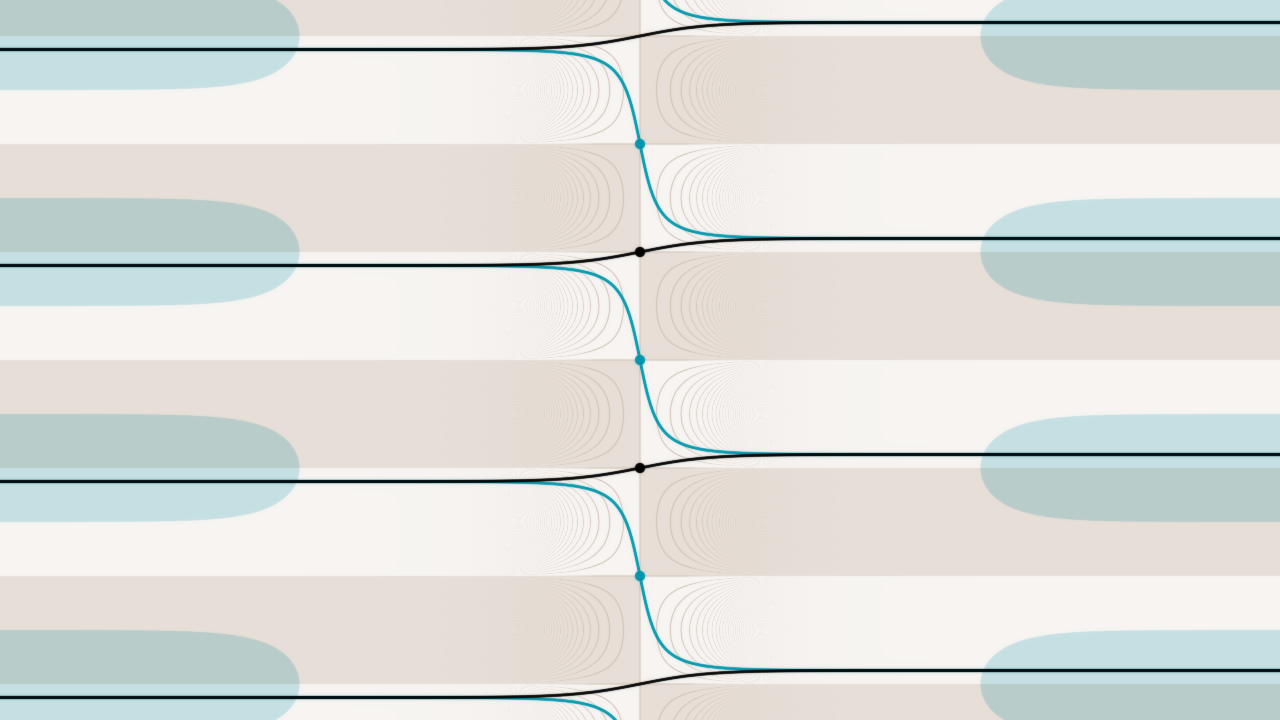
\includegraphics[width=10cm]{figures/bessel-unrolled.png}
\captionof{figure}{The paths $\mathcal{C}^{\pi/8}_j$ in the $t$ plane.}\label{fig:bessel_unrolled}
\end{center}

For any $\mu \in \C \smallsetminus \Z$, the classical modified Bessel function $K_\mu(z)$ can be expressed as the thimble integral
\begin{equation}\label{int:mod-bessel-gen}
 K_\mu(z) = \frac{1}{2 \sinh(\mu\,i\pi)} \int_{\mathcal{C}^\theta_1} \exp\left[z \cosh(t)\right]\,\sinh(\mu t)\,dt
\end{equation}
for $|\theta| < \tfrac{\pi}{2}$. This formula can be deduced, with a lot of finagling, from formulas 10.32(ii) and 10.27.4 of \cite{dlmf}\begin{todo}{[Cite Watson too?]}\end{todo}.
\begin{verify}
\par
From equation~6.22(3) of Watson's \textit{A treatise on the theory of Bessel functions} (1944), p. 181 (the reference in \cite{dlmf}):
\begin{align*}
2\pi i \, I_\mu(z) &= \int_{+\infty}^0 e^{z\cosh(-\pi i+a)-\mu(-i\pi +a)}\,da + \int_{0}^{+\infty} e^{z\cosh(\pi i+a)-\mu(i\pi +a)}\,da +\int_{-\pi}^{\pi} e^{z\cosh(ib)-\mu i b}\,db\\
& = -\int_{-\infty}^0 e^{z\cosh(-\pi i-a)+\mu(i \pi +a)}\,da + \int_{0}^{+\infty} e^{z\cosh(\pi i+a)-\mu(i \pi  +a)}\,da +\int_{0}^{\pi} e^{z\cosh(ib)}\cosh(i\mu b)\,db\\
& = -\int_{-\infty}^0 e^{z\cosh(\pi i+a)+\mu(i\pi +a)}\,da + \int_{0}^{+\infty} e^{z\cosh(\pi i+a)-\mu(i\pi +a)}\,da +\int_{0}^{\pi} e^{z\cosh(ib)}\cosh(i\mu b)\,db.
\end{align*}
Hence,
\begin{align*}
4 i \sin(\mu \pi) K_\mu(z) & = 2\pi i \big[ I_{-\mu}(z) - I_\mu(z) \big] \\
& = \int_{-\infty}^0 e^{z\cosh(\pi i+a)}\left[-e^{-\mu(i\pi +a)}+e^{\mu(i\pi +a)}\right]\,da + \int_{0}^{+\infty} e^{z\cosh(\pi i+a)}\left[e^{\mu(i\pi +a)}-e^{-\mu(i\pi +a)}\right]\,da \\
& \textcolor{OrangeRed}{= 2\int_{-\infty}^0 e^{z\cosh(\pi i+a)} \sinh\big(\mu(a+i\pi)\big)\,da + 2\int_{0}^{+\infty} e^{z\cosh(\pi i+a)} \sinh(\mu(i\pi+a)\big)\,da} \\
& = 2\int_{-\infty}^0 e^{z\cosh(-\pi i+a)} \sinh\big(\mu(a-i\pi)\big)\,da + 2\int_{0}^{+\infty} e^{z\cosh(\pi i+a)} \sinh\big(\mu(i\pi+a)\big)\,da
\end{align*}
\color{OrangeRed}
Stop at the highlighted line! This simplifies to the integral
\[ 2 \int_\gamma e^{z\cosh(t)} \sinh(\mu t)\,dt \]
along the contour $\gamma$ that runs rightward along $i\pi + \R$. \textcolor{magenta}{The integral on the next line is {\em not} the path coming from infinity along $(-\infty,0) + 2\pi i (j - \tfrac{1}{2})$ and returning to infinity along $(0, \infty) + 2\pi i (j + \tfrac{1}{2})$, because it skips the segment along $i(-\pi, \pi)$.}
\par
\end{verify}
The integral converges when $z$ is in the right half-plane. Choosing a rational parameter $\mu = \tfrac{m}{n}$ gives formula~\eqref{integral:mod-bessel-lifted}, showing that $K^{(j)}_{m/n}(z)$ is the classical modified Bessel function $K_{m/n}(z)$ when $j$ is odd.

\color{RoyalBlue}
We can now follow Section \ref{contour-argument-AL} to compute the Borel transform of the asymptotic of $K_\mu$ as an inverse Laplace transform: let $\zeta=-\cosh(t)$
\color{black}
\textcolor{orange}{[\ldots]} We first recast the integral into the $\zeta$ plane by setting $-\zeta = \cosh(t)$
\[ K^{(j)}_{m/n}(z) = -\frac{1}{2\sinh\big(\tfrac{m}{n}\,i\pi\big)} \int_{\mathcal{J}^\theta_{\zeta, \mp 1}} e^{-z\zeta} \left[ \frac{\sinh(\mu t_+)}{\sinh(t_+)} - \frac{\sinh(\mu t_-)}{\sinh(t_-)} \right] d\zeta, \]
where $t_-$ and $t_+$ are the lifts to the incoming and outgoing branches of $\mathcal{C}^\theta_j$. \textcolor{orange}{[\ldots]}
\color{RoyalBlue}
\begin{align*}
    K_\mu(z)& = -\frac{1}{2 \sinh(\mu\,i\pi)} \int_{\gamma_z} e^{-z \zeta}\,\frac{\sinh(\mu t)}{\sinh(t)}\,d\zeta  & \\
    &=-\frac{\mu}{2 \sinh(\mu\,i\pi)} \int_{\gamma_z} e^{-z \zeta}\, {}_2F_1\left(\frac{1+\mu}{2},\frac{1-\mu}{2};\frac{3}{2};1-\zeta^2\right)\,d\zeta & \cite[15.4.16]{dlmf}
\end{align*}
where $\gamma_z$ is Hankel contour coming from $\infty$ to $1$ and then going back to $\infty$. Using formula \cite[15.8.4]{dlmf}, followed by \cite[15.8.27]{dlmf} and \cite[15.8.28]{dlmf} \textcolor{PaleVioletRed}{[Please clean up operators that are repeated across line breaks, like the $=$ below. I like the equation spacing in the ``Thimble projection reasoning for Airly-Lucas functions'' section; can we copy that here?]}
\begin{multline*}
     {}_2F_1\left(\frac{1+\mu}{2},\frac{1-\mu}{2};\frac{3}{2};1-\zeta^2\right) \textcolor{magenta}{=} \\
     =\frac{3}{2}\, {}_2F_1\left(1-\mu,1+\mu,\frac{3}{2};\frac{1-\zeta}{2}\right)+\frac{1}{2}\, {}_2F_1\left(1-\mu,1+\mu,\frac{3}{2};\frac{1+\zeta}{2}\right)
\end{multline*}
hence 
%
\[K_\mu(z)=\frac{\mu\, i}{4 \sin(\mu\pi)} \int_{\gamma_z} e^{-z \zeta}\, {}_2F_1\left(1-\mu,1+\mu;\frac{3}{2};\frac{1+\zeta}{2}\right)\,d\zeta\]
%
Equation \cite[15.2.3]{dlmf} gives the analytic continuation of hypergeometric functions across the branch cut:

\begin{align}
    K_{\mu}(z)& \label{eqn:K-mu}=-\frac{1}{2}\int_1^\infty e^{-z\zeta} \, \left(\frac{\zeta-1}{2}\right)^{-1/2} \,\, {}_2F_1\left(\frac{1}{2}-\mu, \frac{1}{2}+\mu;\frac{1}{2};\frac{1-\zeta}{2}\right)  d\zeta\\
    &  \notag=-\frac{i}{2}\laplace_{\zeta,1} v_{\mu,1} . 
\end{align}
\color{black}
\subsubsection{The case $\mu=0$}
When $\mu$ goes to $0$, formula~\eqref{int:mod-bessel-gen} becomes
\[ K_0(z) = \frac{1}{2\pi i} \int_ {\textcolor{orange}{\Omega}} \exp\left[z \cosh(t)\right]\,t\,dt. \]
\textcolor{orange}{Choosing $\Omega$ to be the unit-speed path that runs from $\infty$ leftward to $-i\pi$, upward to $i\pi$, and rightward back to $\infty$,} we can rewrite this formula as
\begin{align*}
K_0(z) & = \frac{1}{2\pi i} \int_0^\infty \exp\left[-z \cosh(t)\right]\,2\pi i\,dt \\
& = \int_0^\infty \exp\left[-z \cosh(t)\right]\,dt \\
& = \int_1^\infty \exp\left[-z\,\tfrac{1}{2}\left(s + \tfrac{1}{s}\right)\right]\,\frac{ds}{s},
\end{align*}
with $s = e^t$. This is a special case of formula~10.32.9 from \cite{dlmf}. Then equation \eqref{eqn:K-mu} gives
\begin{equation}\label{eqn:borel_bessel0}
    K_0(z)=\textcolor{red}{-}\frac{1}{2}\int_1^\infty e^{-z\zeta} \, \left(\frac{\zeta-1}{2}\right)^{-1/2} \,\, {}_2F_1\left(\frac{1}{2}, \frac{1}{2};\frac{1}{2};\frac{1-\zeta}{2}\right)  d\zeta =  \int_1^\infty \frac{e^{-z\zeta}}{\sqrt{\zeta^2-1}} \, d\zeta .
\end{equation}
\begin{verify}
    We can also verify equation \eqref{eqn:borel_bessel0} using the thimble projection reasoning: from the expression of $K_0$ 
    \begin{equation}
        K_0(z)=\int_0^{\infty} \exp(-z\cosh(t)) dt
    \end{equation}
    we set $\zeta=\cosh(t)$, and choosing a branch for the square root
    \begin{align*}
        d\zeta & = \sinh(t) dt\\
        & =  \sqrt{\zeta^2-1} \, dt
    \end{align*}
    we finally get 
    \[\int_1^{\infty} e^{-z\zeta} \frac{d\zeta}{\sqrt{\zeta^2-1}}\]
\end{verify}



\subsection{Generalized Airy}
In \cite{Reid} and the appendix of \cite{drazin-reid}, Drazin and Reid construct approximate solutions of the Orr--Sommerfield fluid equation using the generalized Airy functions
\begin{align*}
\mathrm{A}_k(y,p) & = \frac{1}{2\pi i}\int_{\mathscr{a}_k} \exp\big[yt-\tfrac{t^3}{3}\big]\,\frac{dt}{t^p} & & p \in \C\hphantom{{}_{\le 0}},\quad k \in \{1,2,3\} \\
\mathrm{B}_0(y,p) & = \frac{1}{2\pi i}\int_{\mathscr{b}_0} \exp\big[yt-\tfrac{t^3}{3}\big]\,\frac{dt}{t^p} & & p \in \Z \\
\mathrm{B}_k(y,p) & = \hphantom{\frac{1}{2\pi i}} \int_{\mathscr{b}_k} \exp\big[yt-\tfrac{t^3}{3}\big]\,\frac{dt}{t^p}, & & p \in \Z_{\le 0},\quad k \in \{1,2,3\}
\end{align*}
which are defined by integrals along the contours $\mathscr{a}_k, \mathscr{b}_0, \mathscr{b}_k$ shown in Figure~\ref{fig:path-generalized-Airy}~\cite{drazin-reid}\cite[Section 9.13(ii)]{dlmf}.
\begin{figure}[ht]
\center
\newcommand{\apathcolor}{ietcoast}
\newcommand{\bpathcolor}{black}
\begin{tikzpicture}
\renewcommand{\dotsize}{0.08}
\fill[pwbeige!10] circle(3.95);
\begin{scope}[\bpathcolor, very thick, -stealth]
  \draw (80:0.8) arc (80:400:0.8);
  \node at (60:0.8) {$\mathscr{b}_0$};
  \foreach \ang/\name in {0/1, 120/2, 240/3} {
    \draw[very thick,-stealth] (0, 0) -- ++(\ang:4) node[anchor=\ang-180] {$\mathscr{b}_\name$};
  };
  \fill (1.25, 0) circle (\dotsize) node[anchor=north west] {$\tfrac{1}{2}$};
  \draw[fill=white, thin] circle (\dotsize);
\end{scope}
\begin{scope}[\apathcolor, very thick, -stealth]
  \foreach \ang/\name in {0/1, 120/2, 240/3} {
    \draw[rotate=\ang] (-0.5, 0) +(-120:3.75) .. controls +(62:1) and +(0, -1.2) .. +(-0.75, 0) .. controls +(0, 1.2) and +(-62:1) .. +(120:3.75) node[midway, anchor=\ang+30] {$\mathscr{a}_\name$};
  };
  \fill (-1.25, 0) circle (\dotsize) node[anchor=north east] {$-\tfrac{1}{2}$};
\end{scope}
\end{tikzpicture}
\caption{The integration contours in the $t$ plane that define $\mathrm{A}_k,\mathrm{B}_0,\mathrm{B}_k$.}\label{fig:path-generalized-Airy}
\end{figure}
These functions satisfy the generalized Airy equation
\[ \left[\big(\tfrac{\partial}{\partial y}\big)^3 - y\,\tfrac{\partial}{\partial y} + (p-1)\right] \Phi = 0. \]
When $p = 0$, this equation reduces to
\[ \tfrac{\partial}{\partial y} \circ \left[\big(\tfrac{\partial}{\partial y}\big)^2 - y\right] \Phi = 0, \]
which is equivalent to an inhomogeneous version of the classical Airy equation.

As we did with the Airy--Lucas functions, we will use the substitution $t = 2uy^{1/2}$ to rewrite the generalized Airy function $\mathrm{A}_1(y,p)$ in terms of a thimble integral. We get
\[ \mathrm{A}_1(y,p) = (12 z)^{(1-p)/3}\,I_+\big(\tfrac{2}{3}y^{3/2},p\big) \]
with
\[ I_+(z,p) = \frac{1}{2\pi i} \int_{\mathcal{C}^\theta_1} \exp\left[-z\left(4u^3 - 3u\right)\right]\,\frac{du}{u^p}. \]
To find the right contour $\mathcal{C}_1^\theta$, we first note that the mapping $\zeta = 4u^3 - 3u$ is familiar, up to a sign, from Section~\ref{sec:airy}. In particular, we already know its critical points $u = \pm\tfrac{1}{2}$ and the corresponding critical values $\zeta = \pm 1$. To get the desired integral, $\mathcal{C}_1^\theta$ should be the thimble through $u = -\tfrac{1}{2}$ over the ray $\mathcal{J}^\theta_1$. However, this thimble does not live on the complex plane, like it did for the classical Airy function. When $p$ is a positive integer, the volume form $du/u^p$ has a pole at $u = 0$, so we put $\mathcal{C}_1^\theta$ as a contour on $\C^\times$. More generally, for any complex value of $p$, we can put $\mathcal{C}_1^\theta$ on the universal cover $\widetilde{\C^\times}$.
\begin{verify}
\begin{align*}
I_{+}(z,p)&=\frac{1}{2\pi i}\int_{\mathcal{C}_{+}}e^{-z(4u^3-3u)}\, \frac{du}{u^p} &\\
&=\frac{1}{2\pi i}(12 z)^{(p-1)/3}\int_{z^{1/3}\mathcal{C}_{+}}e^{-z(\tfrac{4}{12}\tfrac{t^3}{z}-3 (12 z)^{-1/3}t)}\frac{dt}{t^p} & u=(12 z)^{-\tfrac{1}{3}}t\\
&=\frac{1}{2\pi i}(12 z)^{(p-1)/3}\int_{z^{1/3}\mathcal{C}_{+}}e^{-\left(\frac{t^3}{3}-(\tfrac{3}{2} z)^{2/3}t\right)}\frac{dt}{t^p} & \\
&=(12 z)^{(p-1)/3}\mathrm{A}_1((\tfrac{3}{2}z)^{2/3},p)
\end{align*}  
\end{verify}
%
We will now show, in the case $p = 1$, that equation~\eqref{eqn:I} has a frame of Borel regular solutions---as long as the constant solution $\mathrm{B}_0(z, 1)$ counts as Borel regular. For $\mathrm{A}_1(y, p)$ to satisfy the generalized Airy equation, $I_+(z,1)$ must satisfy the equation
\begin{equation}\label{eqn:I}
\left[\big[\big(\tfrac{\partial}{\partial z}\big)^2 - 1\big] + z^{-1} \left(\tfrac{\partial}{\partial z}\right)^2 - \tfrac{1}{9} z^{-2} \right] \tfrac{\partial}{\partial z} \Phi = 0.
\end{equation}
Equivalently, $\tfrac{\partial}{\partial z} I_+(z, 1)$ satisfies the modified Bessel equation \eqref{eqn:reg-mod-bessel-AL} with parameter $1/3$. We can now follow the reasoning of Section~\ref{big-idea}, viewing that frequency domain differential equation~\eqref{eqn:I} as the image under $\laplace_{\zeta, \alpha}$ of the position domain integral equation
\begin{equation}\label{int-eq:position-I}
\left[ \big[ \zeta^2 - 1 \big] - \fracderiv{-1}{\zeta}{\alpha} \circ \zeta - \big(\tfrac{1}{3}\big)^2 \fracderiv{-2}{\zeta}{\alpha} \right] (-\zeta)\,v^{(1)} = 0.
\end{equation}
In Sections \ref{pos-root-AL} and \ref{neg-root-AL}, we found solutions $v_{\pm 1}$ of the closely related equation~\eqref{int-eq:spatial-mod-bessel-AL}, which we can turn into solutions $v^{(1)}_{\pm 1} = \zeta^{-1} v_{\pm 1}$ of equation~\eqref{int-eq:position-I}.

At the critical values $\zeta = \pm 1$, we can build solutions $v^{(1)}_{\pm 1}$ of this equation from the solutions $v_{\pm 1}$ of equation~\eqref{int-eq:spatial-mod-bessel-AL} that we found in Sections \ref{pos-root-AL} and \ref{neg-root-AL}. Explicitly, in terms of the coordinates defined by $\zeta = 1 + \zeta_1$ and $\zeta = -1 + \zeta_{-1}$, these solutions are
\begin{alignat*}{3}
v^{(1)}_1 &=\;& -i\sqrt{2}\,(1 + \zeta_1)^{-1} &\,\zeta_1^{-1/2} &\;{}_2F_1\big(\tfrac{1}{6},\tfrac{5}{6};\tfrac{1}{2};-\tfrac{1}{2}\zeta_{1}\big) \\
v^{(1)}_{-1} &=\;& \sqrt{2}\,(-1 + \zeta_{-1})^{-1} &\,\zeta_{-1}^{-1/2} &\;{}_2F_1\big(\tfrac{1}{6},\tfrac{5}{6};\tfrac{1}{2};\tfrac{1}{2}\zeta_{-1}\big).
\end{alignat*}
Their Laplace transforms $V^{(1)}_1 = \laplace_{\zeta, 1} v^{(1)}_1$ and $V^{(1)}_{-1} = \laplace_{\zeta, -1} v^{(1)}_{-1}$ satisfy equation~\eqref{eqn:I}.
\begin{verify}
From the result about the Bessel equation, we know there exists two analytic functions $v_1$ and $v_{-1}$ such that $\varphi_1$ and $\varphi_2$ defined by $\partial_z\varphi_1=\laplace_{\zeta,1}v_1$ and $\partial_z\varphi_2=\laplace_{\zeta,-1}v_{-1}$, give a frame of analytic solutions of \eqref{eqn:I}. Then we argue as follows:
\begin{align*}
    \partial_z\varphi_1&=\laplace_{\zeta,1}v_1\\
    \varphi_1-\varphi_1(a)&=\int_a^z\int_1^{\infty}e^{-y\zeta} v_1 d\zeta \, dy\\
    &=\int_1^{\infty}d\zeta\,  v_1 \, \int_a^ze^{-y\zeta}  \, dy\\
    &=\int_1^{\infty}d\zeta\,  v_1 \, \Big[\frac{e^{-\zeta a}}{\zeta}-\frac{e^{-z\zeta}}{\zeta}\Big]\\
    &=\laplace_{\zeta,1} \tfrac{v_1}{\zeta}-\Big[\laplace_{\zeta,1}\tfrac{v_1}{\zeta}\Big](a)
\end{align*}
\end{verify}
Notice that $v^{(1)}_1$ belongs to $\singexpalg{-1/2}(\Omega_1)$, has a simple pole at $\zeta_1 = -1$, and has a logarithmic singularity at $\zeta_1 = -2$. Similarly, $v^{(1)}_{-1}$ belongs to $\singexpalg{1/2}(\Omega_{-1})$, has a simple pole at $\zeta_{-1} = 1$, and has a logarithmic singularity at $\zeta_{-1} = 2$.

With an argument analogous to the one in Section~\ref{bessel-regularity-AL}, one should be able to show that $V^{(1)}_1$ and $V^{(1)}_{-1}$ are Borel regular. Since equation~\eqref{eqn:I} is third-order, we need one more Borel regular solution to make a frame. We choose the constant solution $1$, which can be seen as the Laplace transform of the formal convolution unit $\delta$ introduced in Section~\ref{sec:borel-laplace-homom}. Interestingly, $1$ is actually the generalized Airy function $\mathrm{B}_0(z,1)$.
%
\begin{todo}
\subsubsection{Thimble projection formula}
In Theorem~\ref{thm:maxim-proof}, we proved a $3/2$-derivative formula to compute the Borel transform of the asymptotics of a thimble integral.
\color{black}
\end{todo}
\subsection{Third-degree thimble integrals}
\color{DarkBlue}
In this section, we consider the thimble integral
\[ I(z) = \int_{\mathcal{C}} e^{-zg}\,du \]
defined by a general third-degree polynomial map $g \maps \C \to \C$. By definition, the Lefschetz thimble $\mathcal{C}$ is a connected component of the preimage of a critical value of $g$. After taking various symmetries into account, we will find that there are essentially only two cases, distinguished by whether $g$ has two distinct critical points or a single degenerate one.
\subsubsection{Symmetries of the integral}\label{sec:int-symm}
First, we step back and consider the completely general thimble integral
\[ J(z) = \int_{\mathcal{C}} e^{-zf}\,\nu \]
defined by an arbitrary holomorphic map $f \maps X \to \C$ and an arbitrary $1$-form $\nu$ on $X$. The affine group of $\C$ acts on $f$ by post-composition, and this action affects $J$ in a simple way. The affine group is generated by two kinds of transformations, which we consider separately.
%%The affine group of $\C$ acts on $f$ by post-composition, and $\C^\times$ acts on $\nu$ by multiplication. These actions both affect $J$ in simple ways. The affine group is generated by two kinds of transformations, which we consider separately.
\begin{itemize}
\item[] \textbf{Translations}

For any $c \in \C$, the translation action $f \mapsto f + c$ on maps corresponds to the action
\[ J(z) \mapsto e^{-cz} J(z) \]
on integrals. This is because
\begin{align*}
\int_\mathcal{C} e^{-z(f + c)}\,\nu & = e^{-cz} \int_\mathcal{C} e^{-zf}\,\nu \\
& = e^{-cz} \int_\mathcal{C} e^{-zf}\,\nu \\
& = e^{-cz} J(z).
\end{align*}
\item[] \textbf{Scaling-rotations}

For any $r \in \C^\times$, the scaling-rotation action $f \mapsto rf$ corresponds to the action
\[ J(z) \mapsto J(rz) \]
on integrals. This is because
\begin{align*}
\int_\mathcal{C} e^{-z(rf)}\,\nu & = \int_\mathcal{C} e^{-(rz)f}\,\nu \\
& = J(rz).
\end{align*}
%%\item[] \textbf{Multiplications}
%%
%%For any $s \in \C^\times$, the multiplication action $\nu \mapsto s\nu$ corresponds to the action
%%\[ J(z) \mapsto s J(z) \]
%%on integrals.
\end{itemize}
Next, we specialize to the case where $X$ is the complex plane, with standard coordinate $u$, and $\nu = du$. The affine group of $\C$ now acts on $f$ by pre-composition as well. To make sure that $\mathcal{C}$ remains a Lefschetz thimble, we act on it simultaneously by the inverse of whatever we precompose with $f$.
\begin{itemize}
\item[] \textbf{Translations}

For any $c \in \C$, pulling $f$ back along the translation $\mathsf{T}_c^* u = u - c$ has no effect on the integral. This is because $du$ is translation-invariant.

\item[] \textbf{Scaling-rotations}

For any $s \in \C^\times$, the scaling-rotation action $\mathsf{M}_s^* u = s^{-1} u$ corresponds to the action
\[ J(z) \mapsto s J(z) \]
on integrals. This is because
\begin{align*}
\int_{\mathsf{M}_{1/s} \mathcal{C}} e^{-z \mathsf{M}_s^* f}\,du & = \int_\mathcal{C} e^{-zf}\,\mathsf{M}_{1/s}^* du \\
& = \int_\mathcal{C} e^{-zf}\,s\,du \\
& = s J(z).
\end{align*}
%%\item[] \textbf{Multiplications}
%%
%%For any $s \in \C^\times$, the multiplication action $\nu \mapsto s\nu$ corresponds to the action
%%\[ J(z) \mapsto s J(z) \]
%%on integrals.
\end{itemize}
\subsubsection{Reduction of the integral}
We now return to our original thimble integral $I(z)$, defined by the third-degree polynomial map
\[ g = a_3 u^3 + a_2 u^2 + a_1 u + a_0, \]
and use the group actions from Section~\ref{sec:int-symm} to reduce it to its two essential cases. Our first move is to bring the polynomial into depressed form by post-composing it with a scaling by $\tfrac{1}{a_3}$ and pre-composing it with a translation by $\tfrac{1}{3} \tfrac{a_2}{a_3}$.
\begin{center}
\begin{tabular}{c|c|c}
\textbf{Symmetry} & \textbf{Resulting polynomial} & \textbf{Resulting integral} \\[2mm]
$\displaystyle f \mapsto f/a_3$ & $\displaystyle u^3 + \frac{a_2}{a_3} u^2 + \frac{a_1}{a_3} u + \frac{a_0}{a_3}$ & $\displaystyle I\left(\frac{z}{a_3}\right)$ \\[5mm]
$\displaystyle \mathsf{T}_{a_2/3a_3}^*$ & $\displaystyle u^3 + pu + q$ & $\displaystyle I\left(\frac{z}{a_3}\right)$ \\[5mm]
\end{tabular}
\end{center}
The coefficients of the depressed polynomial are given by the usual formulas,\footnote{\begin{align*}
p & = \frac{a_1}{a_3} - \frac{1}{3} \left(\frac{a_2}{a_3}\right)^2 \\
q & = \frac{a_0}{a_3} - \frac{1}{3} \frac{a_1 a_2}{a_3^2} + \frac{2}{27} \left(\frac{a_2}{a_3}\right)^3
\end{align*}}
and its critical points are $\pm\big(\tfrac{p}{3}\big)^{1/2}$. We make the critical values symmetric around $0$ by post-composing the polynomial with a translation by $-q$.
\begin{center}
\begin{tabular}{c|c|c}
\textbf{Symmetry} & \textbf{Resulting polynomial} & \textbf{Resulting integral} \\[2mm]
$\displaystyle f \mapsto f - q$ & $\displaystyle u^3 + pu$ & $\displaystyle e^{qz}\,I\left(\frac{z}{a_3}\right)$ \\[5mm]
\end{tabular}
\end{center}
What we do next depends on how many critical points $g$ has.
\begin{itemize}
\item[] \textbf{Two distinct critical points}

When $p$ is non-zero, $g$ has two distinct critical points. We bring them to $\pm \tfrac{1}{2}$ by pre-composing the polynomial with a scaling by $2\big(\tfrac{p}{3}\big)^{1/2}$. Then we bring the critical values to $\pm 1$ by post-composing with
\begin{center}
\begin{tabular}{c|c|c}
\textbf{Symmetry} & \textbf{Resulting polynomial} & \textbf{Resulting integral} \\[2mm]
$\displaystyle \mathsf{M}_{-2i(p/3)^{1/2}}^*$ & $\displaystyle 2i\left(\frac{p}{3}\right)^{3/2} \left(4u^3 - 3u\right)$ & $\displaystyle -2i\left(\frac{p}{3}\right)^{1/2} e^{qz}\,I\left(\frac{z}{a_3}\right)$ \\[5mm]
$f \mapsto \frac{1}{2i} \left(\frac{3}{p}\right)^{3/2} f$ & \\[5mm]
\end{tabular}
\end{center}
\end{itemize}

\color{black}

\par\color{RoyalBlue}
Let $f\colon\C\to \C$ be a degree three polynomial\footnote{Every degree three polynomial $a_3 u^3+a_2 u^2+a_1 u+a_0$ can be written in the form $a_3u^3+pu+q$, after a change of coordinates $u\to u-\frac{a_2}{3 a_3}$. Furthermore, we can restrict to monic polynomials by setting $a_3=1$.}, we are going to consider thimble integrals of the form 
\[ I_j(z) = \int_{\mathcal{C}_j} \exp\left[z\big(u^3 + pu + q)\right]\,du \]
where $\mathcal{C}_j$ is a thimble in \textcolor{magenta}{$H_{1}^{B,z}$} through a critical point of $f$. We can distinguish between the case when $f$ has two distinct critical points $x_+, x_-$ and only one critical point $x$, which correspond respectively to the case $p\neq 0$ and $p=0$. \footnote{Equivalently, the difference between the generic case ($p\neq 0$) and the degenerate one ($p=0$) is visible from the ODE perspective as in the former case $I$ is a solution of degree two ODE \[\left[\partial_z^2 +2q \partial_z+\left(\frac{4p^3}{27}+q^2\right)+\frac{1}{z}\left(\partial_z +q \right)-\frac{1}{9z^2}\right]\Phi=0,\] while in the latter, $I$ solves a degree one ODE (see \eqref{eqn:degree-3-poly-1root}).}
\color{black}
Recall that translations and scaling-rotations act naturally on the image of $f\colon X\to \C$ ($f$ not necessarily a degree three polynomial), and their action transforms the thimble integral $I_j$ in the following ways:
\begin{itemize}
    \item \textbf{Action of translations:} let $q\in\C$, post-composing with translation of $q$ maps $f\to f+q$, thus 
    \begin{align*}
        \int_{\mathcal{C}_j}e^{z (f+q)} \nu &= e^{qz} I_j(z)
    \end{align*}
    \item  \textbf{Action of scaling-rotations:} let $\gamma\in\C$, post-composing with scaling-rotations by $\gamma$ maps $f\to \gamma\cdot f$, thus 
    \begin{align*}
        \int_{\mathcal{C}_j}e^{z (\gamma\cdot f)} \nu &= I_j(z \gamma)
    \end{align*}
\end{itemize}
In particular, we can always reduce to study the thimble integral in simpler situations. 
As an example, every degree three polynomial with distinct critical points can be transformed in the Chebyshev polynomial $T_3(t)=4 t^3-3t$, implying that the thimble integral $I_+$ can be transformed into the Airy--Lucas integral with parameter $m=1, n=3$. This follows by post-composing $f$ with a translation of $-q$ followed by a scaling-rotation of $\frac{ -i 3^{3/2}}{2 p^{3/2}}$
\begin{align*}
    f-q &= u^3 + pu \\
    (f-q) \cdot \frac{ -i 3^{3/2}}{2 p^{3/2}} &= 4 \Big(\sqrt{-\tfrac{3}{p}} \tfrac{u}{2} \Big)^{3} - 3\Big(\sqrt{-\tfrac{3}{p}} \tfrac{u}{2} \Big) \\
    &= 4 t^3- 3t 
\end{align*}
with $t= \sqrt{-\frac{3}{p}} \frac{u}{2}$. Then the thimble integral $I_+$ gets transformed into 
\begin{align*}
    e^{-zq} I_+\left(-\tfrac{i 3^{3/2}}{2 p^{3/2}} z\right)&= \int_{\mathcal{C}_+} e^{z (4t^3-3t)} du\\
    &= 2\sqrt{-\tfrac{p}{3}} \int_{\mathcal{C}_+} e^{z (4t^3-3t)} dt \\
    &= 2\sqrt{-\tfrac{p}{3}} K_{1/3}(z). 
\end{align*}
In particular, when $p\neq 0$, the thimble integral $I_+$ can be studied following the analysis of Appendix \ref{airy-appendix}. 
%In both cases, we will compute the differential equation satisfied by $I$. 

%\begin{lemma}
 %Let $f(u)=u^3+pu+q$, 
  %  \begin{itemize}
   %     \item if $p\neq 0$, then $I_{\pm}(z)$ solves 
    %    \begin{equation}\label{eqn:degree-3-poly-2roots}
    %        \left[\partial_z^2 +2q \partial_z+\left(\frac{4p^3}{27}+q^2\right)+\frac{1}{z}\left(\partial_z +q \right)-\frac{1}{9z^2}\right]\Phi=0
    %    \end{equation}
    %    \item  if $p=0$, then $I(z)$ solves
     %   \begin{equation}\label{eqn:degree-3-poly-1root}
      %      \left[\partial_z+q+\frac{1}{3z}\right]I=0
      %  \end{equation}
    %\end{itemize}
%\end{lemma}
%\begin{proof}
 %   The proof follows from a direct computation. 
%\end{proof}

%Let us first assume $p\neq 0$, then $x_{\pm}=\pm\sqrt{-p/3}$ and the critical values are $\alpha_{\pm}=f(x_\pm)$. Notice that equation \eqref{eqn:degree-3-poly-2roots} admits slight solutions as $\tau_\pm=\frac{1}{2}$ (recall the definition of $\tau\pm=\frac{Q(-\alpha_\pm)}{P'(-\alpha_\pm)}$ as in Section \ref{borel_reg-ODE}), thus, for $\theta=-\arg z$, $\laplace_{\zeta,f(\alpha_\pm)}^{\theta}v_\pm$ solves \eqref{eqn:degree-3-poly-2roots} if and only $v_\pm$ solves   

%\begin{equation}\label{eqn:deg3-borel-ODE}
 %   \left[\Big[\zeta^2-2q\zeta+\big(\frac{4p^3}{27}+q^2\big)\Big]\partial_\zeta^2+3(\zeta-q)\partial_\zeta+\frac{8}{9}\right]v_\pm=0
%\end{equation}

%Let us find a solution of \eqref{eqn:deg3-borel-ODE} slight at $\zeta=\alpha_+$: in the new coordinate $\zeta_+:=\zeta-\alpha_+$, equation \eqref{eqn:deg3-borel-ODE} becomes

%\begin{equation*}
 %   \left[\zeta_+ (\zeta_+ + \frac{4}{3}p\, x_+)\partial_{\zeta_+}^2+ \left[2p\, x_++3\zeta_{+}\right]\partial_{\zeta_+} +\frac{8}{9} \right]v_+=0
%\end{equation*}

%which is an hypergeometric equation in the coordinate $\xi=-\frac{3}{4p\,x_+}\zeta_+$

%\begin{equation*}
 %   \left[\xi (1-\xi)\partial_{\xi}^2+ 3\big(\frac{1}{2}-\xi\big)\partial_{\xi}-\frac{8}{9} \right]v_+=0
%\end{equation*}

%and it admits a slight solution \textcolor{red}{the solution should match with the one of airy, so choose $w_2$ in DLMf list and not $w_1$}

%\begin{align*}
 %   v_+ &= \xi^{-1/2}\, {}_2F_1\left(\frac{1}{6},\frac{5}{6} ;\frac{3}{2};1-\xi\right)\\
  %  &=\left(\frac{3}{4p\,x_+}\zeta_+\right)^{-1/2}\, {}_2F_1\left(\frac{1}{6},\frac{5}{6} ;\frac{3}{2};1-\frac{3}{4p\,x_+}\zeta_+\right). 
%\end{align*}

%Notice that $v_+$ is a hypergeometric function with the same parameters as the hypergeometric function $v_1$ in the example of Airy \S \ref{pos-root}. Similarly for $\zeta_-=\zeta-\alpha_-$ 

%\begin{equation*}
%    v_- =\left(\frac{3}{4p\,x_-}\zeta_-\right)^{-1/2}\, {}_2F_1\left(\frac{1}{6},\frac{5}{6} ;\frac{3}{2};1-\frac{3}{4p\,x_-}\zeta_-\right). 
%\end{equation*}
We then consider the case when $p=0$, and we study it both as a solution of an ODE and as a thimble integral.
First, notice that $I(z)$ solves
       \begin{equation}\label{eqn:degree-3-poly-1root}
          \left[\partial_z+q+\frac{1}{3z}\right]I=0
       \end{equation}
and we can find a Borel regular solution following the argument of Section~\ref{big-idea}: $\laplace_{\zeta,\alpha}^{\theta}v$ is a solution of \eqref{eqn:degree-3-poly-1root} if and only if $v$ is a solution of 
\begin{align*}
   \left[ (\zeta-q)\partial_\zeta +\frac{2}{3}\right] v=0
\end{align*}
namely $v=(\zeta-q)^{-2/3}=\zeta_q^{-2/3}={}_2F_1\left(a,\frac{2}{3};a;1-\zeta_q\right)$, where $\zeta_q=\zeta-q$ and $a\in\C$ is a free parameter. 

The result is confirmed by the thimble projection reasoning which in this simple case reads
\begin{align*}
    \int_{\mathcal{C}} e^{-z (u^3+q)} du &= e^{-zq} e^{i\pi/3} \int_0^{+e^{i\theta}\infty} e^{-z\zeta} \zeta^{-2/3} d\zeta\\
    &= e^{i\pi/3} \int_q^{+e^{i\theta}\infty} e^{-z\zeta} \, \zeta_q^{-2/3}\,  d\zeta
\end{align*}
where $e^{\pi i/3}$ accounts for the monodromy of $\zeta^{-2/3}$ at the origin. 
\begin{remark}
    The degenerate case $p=0$ can be recovered from the generic case, taking the limit of $I_+(z)$ as $p\to 0$. Indeed, 
    \[ e^{-zq} I_+(z)=2 \sqrt{-\frac{p}{3}} K_{1/3}\Big(\frac{2p^{3/2}}{i3^{3/2}}z\Big)\]
    and its limit as $p\to 0$ can be computed from equations 10.25.2 and 10.27.4 in \cite{dlmf} giving 
    \[ e^{\pi i/3} \Gamma\big(\tfrac{1}{3}\big) e^{-zq} z^{-1/3}.  \]
    \begin{verify}
        \begin{align*}
            2\sqrt{\frac{-p}{3}} K_{1/3}\Big(\frac{2ip^{3/2}}{3^{3/2}}z\Big)&=2\sqrt{\frac{-p}{3}}\left[\frac{\pi}{2\sin(\pi/3)}\Big(I_{-1/3}\big(\tfrac{2ip^{3/2}}{3^{3/2}}z\big)-I_{1/3}\big(\tfrac{2ip^{3/2}}{3^{3/2}}z\big)\Big)\right]\\
            &=\frac{2}{3}\pi ip^{1/2}\left[\Big(\frac{ip^{3/2}}{3^{3/2}}z\Big)^{-1/3}\sum_{k\geq 0}\frac{(-\tfrac{p^3}{3}z^2)^k}{k!\Gamma(k+\tfrac{2}{3})}-\Big(\frac{ip^{3/2}}{3^{3/2}}z\Big)^{1/3}\sum_{k\geq 0}\frac{(-\tfrac{p^3}{3}z^2)^k}{k!\Gamma(k+\tfrac{4}{3})}\right]\\
            &=\frac{2\pi}{\sqrt{3}} e^{\pi i/3} z^{-1/3} \sum_{k\geq 0}\frac{(-\tfrac{p^3}{3}z^2)^k}{k!\Gamma(k+\tfrac{2}{3})}-\frac{2\pi }{3\sqrt{3}} e^{2\pi i/3} z^{1/3} p \sum_{k\geq 0}\frac{(-\tfrac{p^3}{3}z^2)^k}{k!\Gamma(k+\tfrac{4}{3})}
        \end{align*}
         Now we take the limit as $p\to 0$ and we find 
         \[\frac{2\pi}{\sqrt{3}} e^{\pi i/3} z^{-1/3} \frac{1}{\Gamma\big(\tfrac{2}{3}\big)}=e^{\pi i/3} \Gamma\big(\tfrac{1}{3}\big) z^{-1/3}\]
    \end{verify}
    From the properties of the Laplace transform, we then deduce
    \[e^{\pi i/3} \Gamma\big(\tfrac{1}{3}\big) e^{-zq} z^{-1/3}= e^{\pi i/3} e^{-qz} \laplace_{\zeta,0}(\zeta^{-2/3}) = e^{\pi i/3} \laplace_{\zeta_{-q},q}(\zeta^{-2/3})\]
    which agrees with the thimble integral representation of $I$ computed above. 
\end{remark}
\subsection{The triangular cantilever}\label{sec:catilever}
A {\em triangular cantilever} is a flexible strip with constant thickness and linearly tapered width, clamped at the broad end so it sticks out horizontally like a diving board.
\begin{center}
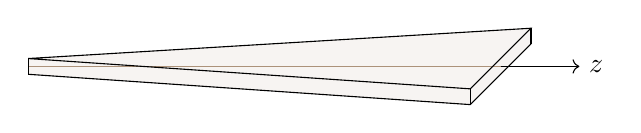
\begin{tikzpicture}
\newcommand{\clen}{6}
\newcommand{\ctaper}{1}
\newcommand{\cthic}{0.1}
\fill[pwbeige!10] (0, \cthic, 0) -- ++(6, 0, -\ctaper) -- ++(0, -2*\cthic, 0) -- ++(0, 0, 2*\ctaper) -- (0, -\cthic, 0);
\draw (0, -\cthic, 0) -- ++(\clen, 0, \ctaper) -- ++(0, 0, -2*\ctaper);
\draw[pwbeige] (0, 0, 0) -- ++(\clen, 0, 0);
\draw[->] (\clen, 0, 0) -- ++(1, 0, 0) node[anchor=west] {$z$};
\draw (0, \cthic, 0) -- ++(\clen, 0, \ctaper) -- ++(0, 0, -2*\ctaper) -- cycle;
\foreach \x / \y in {0 / 0, 6 / 1, 6 / -1} {
  \draw (\x, 0.1, \y) -- (\x, -0.1, \y);
}
\end{tikzpicture}
\end{center}
If you strike the strip from above, it vibrates up and down. Let us suppose the vibrations are small, and uniform across the width of the strip, so we can describe them using the Euler--Bernoulli beam model~\cite[\S 12.4]{genta2009vibration}. The vibration modes of frequency $\omega$ are described by the vertical displacement profiles $\Phi$ that satisfy the equation
\begin{equation}\label{eqn:triangular_cantilever}
    \left[\big[\big(\tfrac{\partial}{\partial z}\big)^4 - \omega^2\big] + \tfrac{2}{z}\big(\tfrac{\partial}{\partial z}\big)^3\right] \Phi = 0,
\end{equation}
where $z$ is the distance from the tip along the strip's axis.\footnote{To keep the equation simple, we've adjusted the units of time so that the strip's elasticity, density, and taper are absorbed into the frequency parameter.}

\begin{verify}
The vertical displacement of a vibrating beam is annihilated by the operator
\[ \big(\tfrac{\partial}{\partial z}\big)^2 \circ EI_\text{roll} \circ \big(\tfrac{\partial}{\partial z}\big)^2 + m \big(\tfrac{\partial}{\partial t}\big)^2, \]
as described in equation~12.58 of \cite{genta2009vibration}. Here, $m$ is the mass per unit length, $E$ is the elastic modulus, and $I_\text{roll}$ is the second moment of area about the axis the beam ``rolls'' around as it vibrates. We can write the displacement as $\cos(\omega t)$ times a time-independent envelope, which is annihilated by the operator
\[ \mathcal{P} = \big(\tfrac{\partial}{\partial z}\big)^2 \circ EI_\text{roll} \circ \big(\tfrac{\partial}{\partial z}\big)^2 - m\omega^2. \]
We are assuming the cantilever has a rectangular cross-section with half-width $s$ and half-thickness $t$, so its second moment of area about the side-to-side axis is $\tfrac{4}{3}st^3$, mass per unit length isproportional to $st$, giving
\[ \mathcal{P} = \big(\tfrac{\partial}{\partial z}\big)^2 \circ \tfrac{4}{3}Et^3 s \circ \big(\tfrac{\partial}{\partial z}\big)^2 - t\omega^2 s. \]
For the triangular cantilever, $t$ is constant, and $s = \sigma z$ for some constant $\sigma$. Letting $c_1 = \tfrac{4}{3}\sigma Et^3$ and $c_2 = t\sigma\omega^2$, we have
\begin{align*}
\mathcal{P} & = \big(\tfrac{\partial}{\partial z}\big)^2 \circ c_1 z \circ \big(\tfrac{\partial}{\partial z}\big)^2 - c_2 z \\
& = c_1 \tfrac{\partial}{\partial z} \circ \big[ 1 + z \tfrac{\partial}{\partial z} \big] \circ \big(\tfrac{\partial}{\partial z}\big)^2 - c_2 z \\
& = c_1 \circ \big[ \tfrac{\partial}{\partial z} + \tfrac{\partial}{\partial z} + z \big(\tfrac{\partial}{\partial z}\big)^2 \big] \circ \big(\tfrac{\partial}{\partial z}\big)^2 - c_2 z \\
& = c_1 2\big(\tfrac{\partial}{\partial z}\big)^3 + c_1 z \big(\tfrac{\partial}{\partial z}\big)^4 - c_2 z \\
\tfrac{1}{c_1 z} \mathcal{P} & = \tfrac{2}{z} \big(\tfrac{\partial}{\partial z}\big)^3 + \big(\tfrac{\partial}{\partial z}\big)^4 - \tfrac{c_2}{c_1}.
\end{align*}
Now, set $\mu = \tfrac{c_2}{c_1} = \tfrac{3}{4} \tfrac{1}{E} \big(\tfrac{\omega}{t}\big)^2$. This example works because the linear density of the beam and the second moment of area about the side-to-side axis are proportional, so they both end up in the $P(\partial/\partial z)$ term.\par
\end{verify}
\color{black}
We are going to look for functions $v$ and points $\zeta = \alpha$ for which the Laplace transform $\laplace_{\zeta, \alpha} v$ satisfies the differential equation~\eqref{eqn:triangular_cantilever}. From Proposition~\ref{prop:L-int-op} we deduce that $\laplace_{\zeta, \alpha} v$ satisfies equation~\eqref{eqn:triangular_cantilever} if and only if $v$ satisfies the integral equation
\begin{equation}\label{eqn:position_cantilever}
    \left[ \big[ \zeta^4 - \omega^2 \big] - 2\fracderiv{-1}{\zeta}{\alpha} \circ \zeta^3 \right] v = 0.
\end{equation}
Observing that
\[ \tfrac{\partial}{\partial \zeta} \sqrt{\zeta^4 - \omega^2} = \frac{2\zeta^3}{\sqrt{\zeta^4 - \omega^2}}, \]
we learn that
\[ v_\text{uni} = \frac{1}{\sqrt{\zeta^4 - \omega^2}} \]
satisfies equation~\eqref{eqn:position_cantilever} whenever $\alpha^4 - \omega = 0$. Thus, a single ``universal solution'' in the position domain leads to four linearly independent solutions $V_\alpha = \laplace_{\zeta, \alpha} v_\text{uni}$ of equation~\eqref{eqn:triangular_cantilever}, indexed by the fourth roots of $\omega^2$.
\par\textcolor{orange}{[Stokes? Thimbles? Mathematica gives solution ${}_0 F_3\big(; \tfrac{1}{2}, \tfrac{3}{4}, \tfrac{3}{4}; \tfrac{1}{16} z^4\big)$.]}
%\subsection{The anharmonic oscillator}\label{sec:anharmonic_oscillator}
%
\appendix
%
\section{The Airy equation}\label{airy-appendix}
%
\subsubsection{Rewriting as a modified Bessel equation}
We can distill the most interesting part of the Airy function by writing
\[ \Ai(y) = \tfrac{1}{\pi\sqrt{3}}\,y^{1/2}\,K\big(\tfrac{2}{3} y^{3/2}\big), \]
where
\begin{equation}\label{integral:mod-bessel}
K(z) = i\sqrt{3} \int_{z^{-1/3}\mathcal{C}_1} \exp\left[z \left(4u^3 - 3u\right)\right]\,du.
\end{equation}
and the contour $\mathcal{C}_1$ is represented in Figure \ref{fig:path_Airy}.
Saying that $\Ai$ satisfies the Airy equation is equivalent to saying that $K$ satisfies the modified Bessel equation
\begin{equation}\label{eqn:mod-bessel-1/3}
\left[z^2 \big(\tfrac{\partial}{\partial z}\big)^2 + z \tfrac{\partial}{\partial z} - \big[\big(\tfrac{1}{3}\big)^2 + z^2\big]\right] K = 0.
\end{equation}
In fact, $K$ is the modified Bessel function $K_{1/3}$~\cite[equation~9.6.1]{dlmf}.
%The method we will demonstrate in Section~\ref{spatial} works for any differential equation
%\[ \left[ P\big(\tfrac{\partial}{\partial z}\big) + z^{-1} Q\big(\tfrac{\partial}{\partial z}\big) + z^{-2} R(z^{-1}) \right] \varphi = 0, \]
%where $P$ is a polynomial, $Q$ is a polynomial of one degree lower, and $R$ is an entire function.
Like we did in equation~\eqref{eqn:reg-mod-bessel-AL}, we can rewrite the modified Bessel equation above as 

\begin{equation}\label{eqn:reg-mod-bessel}
\left[ \big[ \big(\tfrac{\partial}{\partial z}\big)^2 - 1 \big] + z^{-1} \tfrac{\partial}{\partial z} - \big(\tfrac{1}{3}\big)^2 z^{-2} \right] K = 0.
\end{equation}
%
\subsection{Asymptotic analysis}
From the general theory of ODE of Poincar\'e rank $1$, we know that the space of trans-series solutions of ~\eqref{eqn:reg-mod-bessel} has a basis of trans-monomials
\[ \{ e^{-\alpha z} z^{-\tau_\alpha}\,\series{W}_\alpha \mid \alpha^2 - 1 = 0 \} \]
where the $\series{W}_\alpha\in\C\llbracket z^{-1} \rrbracket$ are formal power series in $z^{-1}$. From equations 10.40.2 and 10.17.1 of \cite{dlmf}, we learn that $K \sim \left(\tfrac{\pi}{2}\right)^{1/2} e^{-z} z^{-1/2}\,\series{W}_1$, with
\begin{equation}\label{bessel-asymp}
\series{W}_1 = 1 - \frac{(\tfrac{1}{6})_1 (\tfrac{5}{6})_1}{2^1 \cdot 1!}\;z^{-1} + \frac{(\tfrac{1}{6})_2 (\tfrac{5}{6})_2}{2^2 \cdot 2!}\;z^{-2} - \frac{(\tfrac{1}{6})_3 (\tfrac{5}{6})_3}{2^3 \cdot 3!}\;z^{-3} + \ldots
\end{equation}
The holomorphic analysis in Section~\ref{spatial} will give us holomorphic solutions
\[ \{ e^{-\alpha z} z^{-\tau_\alpha}\,W_\alpha \mid \alpha^2 - 1 = 0 \}, \]
which seem analogous to the trans-monomials above. Borel summation makes the analogy precise. We’ll see in Section~\ref{bessel-regularity} that each $z^{-\tau_\alpha}\,W_\alpha$ is proportional to the Borel sum of $z^{-\tau_\alpha}\,\series{W}_\alpha$. This is an evidence of \cite[Theorem~4]{reg-sing-volterra}.
%
\subsection{Building a distinguished frame of analytic solutions}
\subsubsection{Going to the spatial domain}\label{spatial}
%\subsubsection{The big idea}\label{big-idea}
We are going to look for functions $v_j$ whose Laplace transforms $\laplace_{\zeta, \alpha_j} v_j$ satisfy equation~\eqref{eqn:reg-mod-bessel}. We’ll succeed when $\alpha^2 - 1 = 0$, and we will see that $K$ is a scalar multiple of $\laplace_{\zeta, 1} v_1$.

From Proposition~\ref{prop:L-int-op}, we find that $\laplace_{\zeta, \alpha} v$ satisfies the differential equation~\eqref{eqn:reg-mod-bessel} if and only if $v$ satisfies the integral equation
\begin{equation}\label{int-eq:spatial-mod-bessel}
\left[ \big[ \zeta^2 - 1 \big] - \fracderiv{-1}{\zeta}{\alpha} \circ \zeta - \big(\tfrac{1}{3}\big)^2 \fracderiv{-2}{\zeta}{\alpha} \right] v = 0.
\end{equation}
It's tempting to differentiate both sides of this equation until we get
\begin{equation}\label{diff-eq:spatial-mod-bessel}
\left[ \big(\tfrac{\partial}{\partial \zeta}\big)^2 \circ \big[ \zeta^2 - 1 \big] - \tfrac{\partial}{\partial \zeta} \circ \zeta - \big(\tfrac{1}{3}\big)^2 \right] v = 0,
\end{equation}
which is easier to solve. However, as we learned in Section~\ref{shifting}, a solution of equation~\eqref{diff-eq:spatial-mod-bessel} satisfies equation~\eqref{int-eq:spatial-mod-bessel} if it is slight and locally integrable at $\zeta = \alpha$. 

This is great news, because equation~\eqref{diff-eq:spatial-mod-bessel} has a regular singularity at each root of $\zeta^2 - 1$, and the Frobenius method often gives a slight solution at each regular singular point. We can see the regular singularities by moving the derivatives to the right:
\[ \left[ (\zeta^2 - 1) \big(\tfrac{\partial}{\partial \zeta}\big)^2 + 3\zeta \tfrac{\partial}{\partial \zeta} + \big[ 1 - \big(\tfrac{1}{3}\big)^2 \big] \right] v = 0. \]
In Sections \ref{pos-root}\,--\,\ref{neg-root}, we will see this approach succeed. For each root $\alpha$, we will find a solution $v_\alpha$ of equation~\eqref{diff-eq:spatial-mod-bessel} which is slight and locally integrable at $\zeta = \alpha$. We know the function $\laplace_{\zeta, \alpha} v_\alpha$ will satisfy equation~\eqref{eqn:reg-mod-bessel}, and we can even find its asymptotics from the order $\tau_\alpha$ of $v_\alpha$. We learned in Section~\ref{translation} that
\[ \laplace_{\zeta, \alpha} v_\alpha = e^{-\alpha z} V_\alpha \]
where $V_\alpha = \laplace_{\zeta_\alpha, 0} v_\alpha$ and $\zeta = \alpha + \zeta_\alpha$. We can see from Section~\ref{sec:reg-decay} that $V_\alpha$ is asymptotic to a scalar multiple of $z^{ - \tau_\alpha}$ at $z = \infty$, so the further decomposition
\[ \laplace_{\zeta, \alpha} v_\alpha = e^{-\alpha z} z^{-\tau_\alpha} W_\alpha, \]
makes $W_\alpha$ is asymptotic to a scalar multiple of $1+O(z^{-1})$ at $z = \infty$.
%\textcolor{Magenta}{Show that $W_1$ is asymptotic to $\tilde{W}_1$!}
%\color{Peru}
%\begin{align*}
%\left[ \big(\tfrac{\partial}{\partial \zeta}\big)^2 \circ (\zeta - 1)(\zeta + 1) - \tfrac{\partial}{\partial \zeta} \circ \zeta - \big(\tfrac{1}{3}\big)^2 \right] v & = 0
%\end{align*}
%\color{Sienna}
%\begin{align*}
%\left[ \big[ 2 + 2(2\zeta) \tfrac{\partial}{\partial \zeta} + (\zeta^2 - 1) \big(\tfrac{\partial}{\partial \zeta}\big)^2 \big] - \big[ 1 + \zeta \tfrac{\partial}{\partial \zeta} \big] - \big(\tfrac{1}{3}\big)^2 \right] v & = 0 \\
%\left[ (\zeta^2 - 1) \big(\tfrac{\partial}{\partial \zeta}\big)^2 + 3\zeta \tfrac{\partial}{\partial \zeta} + \big[ 1 - \big(\tfrac{1}{3}\big)^2 \big] \right] v & = 0 \\
%\left[ (\zeta - 1)(\zeta + 1) \big(\tfrac{\partial}{\partial \zeta}\big)^2 + 3\zeta \tfrac{\partial}{\partial \zeta} + \big[ 1 - \big(\tfrac{1}{3}\big)^2 \big] \right] v & = 0
%\end{align*}
%\color{black}
%%In terms of the coordinate $\zeta_\alpha$ with $\zeta = \alpha + \zeta_\alpha$, this equation is written
%%\begin{equation}\label{eqn:centered-mod-bessel}
%%\[ \left[ \big[ \zeta_\alpha (\zeta_\alpha + 2\alpha) + \alpha^2 - 1 \big] + \fracderiv{-1}{\zeta_\alpha}{0} \circ \big[ \zeta_\alpha + \alpha \big] - \big(\tfrac{1}{3}\big)^2 \fracderiv{-2}{\zeta_\alpha}{0} \right] w = 0. \]
%%\end{equation}
\subsubsection{Focus on $\zeta = 1$}\label{pos-root}
Let us find a solution of equation~\eqref{diff-eq:spatial-mod-bessel} which is slight and locally integrable at $\zeta = 1$. Define a new coordinate $\zeta_1$ on $\C$ so that $\zeta = 1 + \zeta_1$. In this coordinate, equation~\eqref{diff-eq:spatial-mod-bessel} looks like
\begin{equation}%%\label{diff-eq:spatial-mod-bessel-pos}
\left[\zeta_1(2 + \zeta_1) \big(\tfrac{\partial}{\partial \zeta_1}\big)^2 + 3(1 + \zeta_1) \tfrac{\partial}{\partial \zeta_1} + \big[1 - \big(\tfrac{1}{3}\big)^2\big]\right] v = 0.
\end{equation}
With another change of coordinate, given by $\zeta_1 = -2\xi_1$, we can rewrite equation~\eqref{diff-eq:spatial-mod-bessel} as the hypergeometric equation
\begin{equation}\label{diff-eq:hypergeom-pos}
\left[\xi_1 (1 - \xi_1) \big(\tfrac{\partial}{\partial \xi_1}\big)^2 + 3(\tfrac{1}{2} - \xi_1) \tfrac{\partial}{\partial \xi_1} - \big[1 - \big(\tfrac{1}{3}\big)^2\big]\right] v = 0.
\end{equation}
Looking through the twenty-four expressions for Kummer's six solutions, we find one \cite[formula~15.10.12]{dlmf} which is manifestly slight and locally integrable at $\xi_1 = 0$:
\begin{alignat*}{2}
v_1 &=\;& \hphantom{-i\sqrt{2}}\,\xi_1^{-1/2} & {}_2F_1\big(\tfrac{1}{6}, \tfrac{5}{6}; \tfrac{1}{2}; \xi_1\big) \\
&=\;& -i\,\left(\frac{\zeta_1}{2}\right)^{-1/2} & {}_2F_1\big(\tfrac{1}{6}, \tfrac{5}{6}; \tfrac{1}{2}; -\tfrac{1}{2}\zeta_1\big)
\end{alignat*}
From the argument in Section~\ref{spatial}, we know that $\laplace_{\zeta, 1} v_1$ satisfies equation~\eqref{eqn:reg-mod-bessel}, and can be written as $e^{-z} V_1$, where $V_1 = \laplace_{\zeta_1, 0} v_1$. Since $v_1$ has order $-1/2$, the decomposition $V_1 = z^{1/2} W_1$ makes $W_1$ asymptotic to a scalar multiple of $z^{-1}$ at $z = \infty$.
\subsubsection{Focus on $\zeta = -1$}\label{neg-root}
Let us find a solution of equation~\eqref{diff-eq:spatial-mod-bessel} which is slight and locally integrable at $\zeta = -1$. In the rescaled coordinate from Section~\ref{pos-root}, this is the point $\xi_1 = 1$. Looking again through Kummer's table of solutions, we find another expression \cite[formula~15.10.14]{dlmf} which is manifestly slight and locally integrable at $\xi_1 = 1$:
\begin{alignat*}{2}
v_{-1} &=\;& (1-\xi_1)^{-1/2} & F\big(\tfrac{1}{6}, \tfrac{5}{6}; \tfrac{1}{2}; 1-\xi_1\big) \\
&=\;& \left(\frac{\zeta_{-1}}{2}\right)^{-1/2} & F\big(\tfrac{1}{6}, \tfrac{5}{6}; \tfrac{1}{2}; \tfrac{1}{2}\zeta_{-1}\big)
\end{alignat*}
where $\zeta_{-1}$ is the coordinate with $\zeta = -1 + \zeta_{-1}$. From the argument in Section~\ref{big-idea}, we know that $\laplace_{\zeta, -1} v_{-1}$ satisfies equation~\eqref{eqn:mod-bessel}, and can be written as $e^z V_{-1}$, where $V_{-1} = \laplace_{\zeta_{-1}, 0} v_{-1}$. Since $v_{-1}$, like our other solution, has order $-1/2$, the same decomposition $V_{-1} = z^{1/2} W_{-1}$ makes $W_{-1}$ asymptotic to a scalar multiple of $z^{-1}$ at $z = \infty$.

In this example, $v_1$ and $v_{-1}$ happen to be related by a symmetry: the M\"{o}bius transformation that pulls $\zeta$ back to $-\zeta$. Kummer's solutions typically come from six different hypergeometric equations, which are related by the M\"{o}bius transformations that permute their singularities. In our case, though, exchanging $1$ with $-1$ keeps equation~\eqref{diff-eq:spatial-mod-bessel} the same.
%\color{DodgerBlue}
%If we follow the routine from Section~\ref{pos-root}, rewriting equation~\eqref{diff-eq:spatial-mod-bessel} in the coordinate $\zeta_{-1}$ and then rewriting it again in a more recognizable form, we arrive at the hypergeometric equation
%\[ \left[\xi_{-1} (1 - \xi_{-1}) \big(\tfrac{\partial}{\partial \xi_{-1}}\big)^2 + 3(\tfrac{1}{2} - \xi_{-1}) \tfrac{\partial}{\partial \xi_{-1}} - \big[1 - \big(\tfrac{1}{3}\big)^2\big]\right] v = 0, \]
%where $\zeta_{-1} = 2\xi_{-1}$. This is the same as what we get by substituting $\xi_{-1}$ for $\xi_1$ in Section~\ref{pos-root}! In other words, the holomorphic map that pulls $\xi_{-1}$ back to $\xi_1$.
\subsection{Borel regularity}\label{bessel-regularity}
Recall that $\tilde{W}_1$ is a formal solution of \eqref{eqn:reg-mod-bessel}
\begin{equation}
\tilde{W}_1(z)=\sum_{n=0}^{\infty}\frac{\left(\frac{1}{6}\right)_n\left(\frac{5}{6}\right)_n}{n!}\frac{(-1)^n}{2^n}z^{-n}.
\end{equation}
Our goal is to prove that the Borel sum of $z^{-1/2}\tilde{W}_1$ is proportional to $V_1=\laplace_{\zeta_1,0}v_1$. 
%
%\subsubsection{Borel sum of $\tilde{W}_1$}
%
%Let us first compute the Borel transform of $\tilde{W}_1$:
%
%
%\begin{align*}
%\tilde{w}_1(\zeta)&=\delta+\sum_{n=1}^{\infty}\frac{\left(\frac{1}{6}\right)_n\left(\frac{5}{6}\right)_n}{n!}\frac{(-1)^n}{2^n}\frac{\zeta^{n-1}}{\Gamma(n)}\\
%&=\delta -\frac{1}{2}\sum_{n=0}^{\infty}\frac{\left(\frac{1}{6}\right)_{n+1}\left(\frac{5}{6}\right)_{n+1}}{\Gamma(n+2)n!}\frac{(-\zeta)^n}{2^n}\\
%&=\delta-\frac{1}{2}\frac{\Gamma(\frac{7}{6})\Gamma(\frac{11}{6})}{\Gamma(\frac{1}{6})\Gamma(\frac{5}{6})}\sum_{n=0}^{\infty}\frac{\left(\frac{7}{6}\right)_{n}\left(\frac{11}{6}\right)_{n}}{\Gamma(n+2)n!}\frac{(-\zeta)^n}{2^n}\\
%&=\delta-\frac{5}{72}\,\, {}_2F_1\left(\frac{7}{6},\frac{11}{6};2,-\frac{\zeta}{2}\right)
%\end{align*}
Let us compute the Borel transform of $z^{-1/2}\tilde{W}_1$: notice that the appropriate coordinate is $\zeta_1$ 
\begin{align*}
\borel\left[z^{-1/2}\tilde{W}_1(z)\right](\zeta_1)&=\borel\left[\sum_{n=0}^{\infty}\frac{\left(\frac{1}{6}\right)_n\left(\frac{5}{6}\right)_n}{n!}\frac{(-1)^n}{2^n}z^{-n-\frac{1}{2}} \right](\zeta_1)\\
&=\sum_{n=0}^{\infty}\frac{\left(\frac{1}{6}\right)_n\left(\frac{5}{6}\right)_n}{n!}\frac{(-1)^n}{2^n}\frac{\zeta_1^{n-\frac{1}{2}}}{\Gamma(n+\frac{1}{2})}\\
&=\zeta_1^{-1/2}\,\, {}_2F_1\left(\frac{1}{6},\frac{5}{6};\frac{1}{2};-\frac{\zeta_1}{2}\right)
\end{align*}
Comparing with the solution $v_1$ computed in Section~\ref{pos-root} we notice that \[v_1(\zeta_1)\propto \borel\left[z^{-1/2}\tilde{W}_1\right](\zeta_1)\]
therefore the Borel Laplace sum of $z^{-1/2}\tilde{W}_1$ is proportional to $V_1$. In particular, both $K$ and $e^{-z}V_1$ are analytic solutions of the Airy equation~\eqref{eqn:reg-mod-bessel} and they have the same asymptotics at $\infty$ up to a multiplicative constant. 

Similarly, if we consider the formal power series
\begin{equation}
\tilde{W}_{-1}(z)=\sum_{n=0}^{\infty}\frac{\left(\frac{1}{6}\right)_n\left(\frac{5}{6}\right)_n}{n!}\frac{1}{2^n}z^{-n}
\end{equation}
analogous computations give that $v_{-1}(\zeta_{-1})\propto\borel\left[z^{-1/2}\tilde{W}_{-1}\right](\zeta_{-1})$.
\subsection{Thimble projection reasoning for the Airy function}\label{contour-argument}
\textcolor{orange}{[Convert to new version]} Generalizing from Section~\ref{contour-argument-AL}, we can recast integral~\eqref{integral:mod-bessel} into the $\zeta$ plane by setting $-\zeta = 4u^3 - 3u$. Projecting $z^{-1/3} \mathcal{C}_1$ to a contour \textcolor{magenta}{[rephrase in terms of ray]} $\mathcal{H}^1_z$ in the $\zeta$ plane and choosing the branch of $u$ that lifts $\mathcal{H}^1_z$ back to $z^{-1/3} \mathcal{C}_1$, we have
\begin{equation}\label{integral:mod-bessel-zeta}
K = \frac{i}{\sqrt{3}} \int_{\mathcal{H}^1_z} e^{-z\zeta}\frac{d\zeta}{4u^2 - 1}.
\end{equation}
For $z \in (0, \infty)$, the contour $\mathcal{H}^1_z$ runs clockwise around $[1, \infty)$, as shown below. Let us assume $z \in (0, \infty)$ for the rest of the section. \textcolor{magenta}{[Our conclusions should probably hold whenever $\operatorname{Re}(z) > 0$.]}
\begin{center}
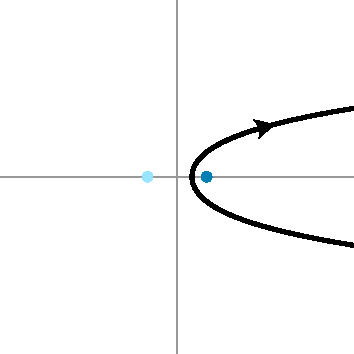
\includegraphics{figures/zeta_contour_3.pdf} \\[1em]
{\small The contour $\mathcal{H}^1_z$ in the $\zeta$ plane.}
\end{center}
From formula~15.4.14 in \cite{dlmf}, we learn that for our desired branch of $u$,
\[ \frac{1}{4u^2 - 1} = -F\big(\tfrac{1}{3}, \tfrac{2}{3}; \tfrac{1}{2}; \zeta^2\big), \]
so we can rewrite integral~\eqref{integral:mod-bessel-zeta} as
\[ K = \frac{1}{i\sqrt{3}} \int_{\mathcal{H}^1_z} e^{-z\zeta} F\big(\tfrac{1}{3}, \tfrac{2}{3}; \tfrac{1}{2}; \zeta^2\big)\;d\zeta. \]
This gives us an alternate route to the conclusion of Section~\ref{spatial}, which we will follow below.

In addition to the solutions $v_1$ and $v_{-1}$ from Sections~\ref{pos-root}\,--\,\ref{neg-root}, equation~\eqref{diff-eq:spatial-mod-bessel} has the solutions
\begin{alignat*}{2}
g_1 &\;=\;& & {}_2F_1\big(\tfrac{2}{3}, \tfrac{4}{3}; \tfrac{3}{2}; \xi_1\big) \\
g_{-1} &\;=\;&  & {}_2F_1\big(\tfrac{2}{3}, \tfrac{4}{3}; \tfrac{3}{2}; 1-\xi_1\big),
\end{alignat*}
given by formulas 15.10.11 and 15.10.13 from \cite{dlmf}.

The quadratic transformation identity 15.8.27 from \cite{dlmf} shows that\footnote{Note that $2\Gamma(\tfrac{1}{2})\Gamma(\tfrac{3}{2}) = 2\Gamma(\tfrac{1}{2})\,\tfrac{1}{2}\Gamma(\tfrac{1}{2}) = \pi$ and $\big[\Gamma(\tfrac{5}{6})\Gamma(\tfrac{7}{6})\big]^{-1} = \big[\Gamma(\tfrac{5}{6})\,\tfrac{1}{6}\Gamma(\tfrac{1}{6})\big]^{-1} = \frac{6\sin(\tfrac{1}{6} \pi)}{\pi} = \frac{3}{\pi}$.}
\[ F\big(\tfrac{1}{3}, \tfrac{2}{3}; \tfrac{1}{2}; \zeta^2\big) = \tfrac{1}{3}(g_1 + g_{-1}), \]
so we have
\[ K = \frac{1}{i\,3\sqrt{3}} \int_{\mathcal{H}^1_z} e^{-z\zeta} (g_1 + g_{-1})\;d\zeta. \]
The solution $g_{-1}$ is holomorphic on $\zeta \in [1, \infty)$, so it integrates to zero. The solution $g_1$, in contrast, is non-meromorphic at $\zeta = 1$. Along the branch cut $\zeta \in [1, \infty)$, its above-minus-below difference is $-\tfrac{3\sqrt{3}}{2}\,v_1$,
as given\footnote{Note that $\Gamma(\tfrac{3}{2}) \Gamma(\tfrac{1}{2})^{-1} = \tfrac{1}{2}$ and $\big[\Gamma(\tfrac{2}{3})\Gamma(\tfrac{4}{3})\big]^{-1} = \big[\Gamma(\tfrac{2}{3})\,\tfrac{1}{3}\Gamma(\tfrac{1}{3})\big]^{-1} = \frac{3\sin(\tfrac{1}{3} \pi)}{\pi} = \frac{3\sqrt{3}}{2\pi}$.} by equation~15.2.3 from \cite{dlmf}.
Hence,
\begin{align*}
K & = \frac{i}{2} \int^\infty_1 e^{-z\zeta} v_1\;d\zeta \\
e^z K & = \frac{i}{2} \int^\infty_1 e^{-z(\zeta - 1)} v_1\;d\zeta \\
e^z K & = \tfrac{i}{2} \laplace_{\zeta_1} v_1,
\end{align*}
just as we found in Section~\ref{bessel-regularity}. However, in this case, we get an exact equality (compared to the proportionality of Section~\ref{bessel-regularity}). 
\subsubsection{Another solution}
Section~\ref{contour-argument} associates the solution $K$ of equation~\eqref{eqn:mod-bessel} with the solution $g_1$ of equation~\eqref{diff-eq:hypergeom-pos}, which contributes the pole at $\zeta = 1$ of
\[ \frac{du}{d\zeta} = \frac{1}{4u^2 - 1} = \tfrac{1}{3}(g_1 + g_{-1}). \]
The solution $g_{-1}$, which contributes the pole at $\zeta = -1$, is associated with another solution of equation~\eqref{eqn:reg-mod-bessel}.
To express this other solution as a Laplace transform, following the method of Section~\ref{contour-argument}, we would use the solution
\[ v_{-1} = (1-\xi)^{-1/2} \,\, {}_2F_1\big(\tfrac{1}{6}, \tfrac{5}{6}; \tfrac{1}{2}; 1-\xi\big) \]
of equation~\eqref{diff-eq:spatial-mod-bessel}, given by formula~15.10.14 from \cite{dlmf}. This is the only solution, up to scale, which has a fractional power singularity at $\zeta = -1$.

In summary, the thimble projection technique of solving equation~\eqref{eqn:reg-mod-bessel} is associated with the basis
\begin{align*}
g_{1} & = {}_2F_1\big(\tfrac{2}{3}, \tfrac{4}{3}; \tfrac{3}{2}; \xi\big) \\
g_{-1} & = {}_2F_1\big(\tfrac{2}{3}, \tfrac{4}{3}; \tfrac{3}{2}; 1-\xi\big)
\end{align*}
of solutions for equation~\eqref{diff-eq:spatial-mod-bessel}, given by formulas 15.10.11 and 15.10.13 from \cite{dlmf}. These solutions contribute the poles at $\xi = 1$ and $\xi = 0$, respectively, of a generic solution.

The Laplace transformation method of solving equation~\eqref{eqn:reg-mod-bessel}, on the other hand, is associated with the basis
\begin{alignat*}{2}
v_{-1} &\;=\;& (1-\xi)^{-1/2} & \, {}_2F_1\big(\tfrac{1}{6}, \tfrac{5}{6}; \tfrac{1}{2}; 1-\xi\big) \\
v_1 &\;=\:& \xi^{-1/2} & \, {}_2F_1\big(\tfrac{1}{6}, \tfrac{5}{6}; \tfrac{1}{2}; \xi\big)
\end{alignat*}
given by formulas 15.10.14 and 15.10.12 from \cite{dlmf}. These solutions, up to scale, are the only ones with fractional power singularities.

Identities 15.10.18, and 15.10.22 from \cite{dlmf} give the change of basis
\begin{alignat*}{3}
v_{-1} &\;=\;&\tfrac{1}{\sqrt{3}}\,g_{-1} &\;+\;& \tfrac{1}{2}\,v_1 \\
v_1 &\;=\;& \tfrac{1}{\sqrt{3}}\,g_{1} &\;+\;& \tfrac{1}{2}\,v_{-1}.
\end{alignat*}
Summing these identities, we see that
\[ g_1 + g_{-1} = \tfrac{\sqrt{3}}{2}\,(f_1 + f_{-1}), \]
giving the alternate decomposition
\[ \frac{du}{d\zeta} = \tfrac{1}{2\sqrt{3}}\,(f_1 + f_{-1}). \]

\subsection{Thimble projection formula}

In the Airy-Lucas integral, $f$ is a Chebyshev polynomial, so we can do a thimble projection technique (see Section~\ref{contour-argument-AL}) or apply the thimble projection formula equation~\eqref{eqn:formula-proof} using trigonometric substitution. As an example of how one might reason in the latter case, we look at the Airy function, given by $f = 4u^3-3u$.

\textcolor{RoyalBlue}{[\ldots] this time applying the thimble projection formula to the generalized Cardano's formula.}

\textcolor{Peru}{Recall that the roots of $f(u)-\zeta$ can be written explicitly as 
\begin{align*}
    u(\zeta)&=\cos\Big(\frac{1}{3}\arccos\zeta-\frac{2\pi k}{3}\Big) \quad k=0,1,2\\
    &={}_2F_1\Big(-\frac{1}{6},\frac{1}{6};\frac{1}{2};1-\zeta^2\Big)
\end{align*}}
\textcolor{orange}{[Add the numerical check to show simple resurgence. For example, maybe graph exponential of the magnitude of function on position domain]}
The thimble $\mathcal{C}_1$ can be parametrized by the path $\theta \mapsto \cosh(\theta - \tfrac{2}{3}\pi i)$. Since $4u^3 - 3u$ is the third Chebyshev polynomial and $\cosh$ is $2\pi$-periodic in the imaginary direction, the start and end points of $\mathcal{C}_1(\zeta)$ are then characterized by
\begin{align*}
u & = \cosh(\mp\theta - \tfrac{2}{3}\pi i) \\
\zeta & = \cosh(3\theta).
\end{align*}
It follows that
\begin{align*}
\int_{\mathcal{C}_1(\zeta)} \nu & = \int_{\mathcal{C}_1(\zeta)} du \\
& = u \Big|_{\operatorname{start} \mathcal{C}_1(\zeta)}^{\operatorname{end} \mathcal{C}_1(\zeta)}\\
 & = \cosh(\theta - \tfrac{2}{3}\pi i) - \cosh(-\theta - \tfrac{2}{3}\pi i) \\
& = \big[\cosh(\theta) \cosh(-\tfrac{2}{3}\pi i) + \sinh(\theta) \sinh(-\tfrac{2}{3}\pi i)\big] \\
& \quad - \big[\cosh(-\theta) \cosh(-\tfrac{2}{3}\pi i) + \sinh(-\theta) \sinh(-\tfrac{2}{3}\pi i)\big] \\
& = 2\sinh(\theta) \sinh(-\tfrac{2}{3}\pi i) \\
& = -i\sqrt{3}\,\sinh(\theta).
\end{align*}
Let $\xi = \tfrac{1}{2}(1 - \zeta)$, and notice that $\xi = -\sinh\big(\tfrac{3}{2} \theta\big)^2$ at the start and end points. The identity~15.4.16 \cite{dlmf}
\[ \sinh( \theta) = \tfrac{1}{3} \sinh\big( \tfrac{3}{2}\theta\big)\,{}_2F_1\big(\tfrac{1}{6}, \tfrac{5}{6}; \tfrac{3}{2}; -\sinh\big(\tfrac{3}{2}\theta\big)^2\big) \]
then shows us that
\[ \frac{i}{\sqrt{3}} \int_{\mathcal{C}_1(\zeta)} \nu = (-\xi)^{1/2}\,{}_2F_1\big(\tfrac{1}{6}, \tfrac{5}{6}; \tfrac{3}{2}; \xi\big). \]

Now we can evaluate the half-integral of $\int_{\mathcal{C}_1} \nu$ using Bateman's fractional integral formula for hypergeometric functions see \cite[Section 4.1]{koornwinder2015fractional}.
\begin{align*}
\fracderiv{-1/2}{\zeta}{1} \left( \int_{\mathcal{C}_1(\zeta)} \nu \right) & = \frac{1}{\Gamma\big(\tfrac{1}{2}\big)} \int_{1}^\zeta (\zeta - \zeta')^{-1/2} \left( \int_{\mathcal{C}_1(\zeta')} \nu \right)\,d\zeta' \\
& = \frac{1}{\Gamma\big(\tfrac{1}{2}\big)} \int_0^\xi  (\xi' - \xi)^{-1/2} \Big[ -{i}{\sqrt{3}}\, (-\xi)^{1/2}\,{}_2F_1\big(\tfrac{1}{6}, \tfrac{5}{6}; \tfrac{3}{2}; \xi\big) \Big] \,\big( -\,d\xi' \big) \\
& = -i \frac{\Gamma\big(\tfrac{3}{2}\big)}{\Gamma(2)} (-\xi)\,{}_2F_1\big(\tfrac{1}{6}, \tfrac{5}{6}; 2; \xi\big) \\
& = \frac{i}{2} \sqrt{\pi}\,\xi\, {}_2F_1\big(\tfrac{1}{6}, \tfrac{5}{6}; 2; \xi\big).
\end{align*}
Finally, we differentiate twice using 15.5.4 and 15.5.1 from \cite{dlmf}.
\begin{align*}
\fracderiv{3/2}{\zeta}{1} \left( \int_{\mathcal{C}_1(\zeta)} \nu \right) & = \left(-\tfrac{\partial}{\partial \xi}\right)^2 \left[ \frac{i\sqrt{\pi}}{2}\,\xi\, {}_2F_1\big(\tfrac{1}{6}, \tfrac{5}{6}; 2; \xi\big) \right] \\
& =  \tfrac{i\sqrt{\pi}}{2} \left(\tfrac{\partial}{\partial \xi}\right)^2 \left[ \xi\,{}_2F_1\big(\tfrac{1}{6}, \tfrac{5}{6}; 2; \xi\big) \right] \\
& = \tfrac{i\sqrt{\pi}}{2}\,\tfrac{\partial}{\partial \xi} \left[ {}_2F_1\big(\tfrac{1}{6}, \tfrac{5}{6}; 1; \xi\big) \right] \\
& = \tfrac{i\sqrt{\pi}}{2}\,\tfrac{5}{12}\, {}_2F_1\big(\tfrac{7}{6}, \tfrac{11}{6}; 2; \xi\big).
\end{align*}
%
For completeness, we repeat the computations for $\hat{\phi}_{-1}$: the thimble $\mathcal{C}_{-1}$ can be parametrized by the path $\theta \mapsto -\cosh(\theta - \tfrac{2}{3}\pi i)$. Hence,
\begin{align*}
\int_{\mathcal{C}_{-1}(\zeta)} \nu & = \int_{\mathcal{C}_{-1}(\zeta)} du \\
& = u \Big|_{\operatorname{start} \mathcal{C}_{-1}(\zeta)}^{\operatorname{end}\mathcal{C}_{-1}(\zeta)}.
\end{align*}
The start and end points of $\mathcal{C}_{-1}$ are characterized by
\begin{align*}
u & = -\cosh(\mp\theta - \tfrac{2}{3}\pi i) \\
\zeta & = -\tfrac{2}{3} \cosh(3\theta),
\end{align*}
so
\begin{align*}
\int_{\mathcal{C}_{-1}(\zeta)} \nu & =- \cosh(\theta - \tfrac{2}{3}\pi i) + \cosh(-\theta - \tfrac{2}{3}\pi i) \\
& =- \big[\cosh(\theta) \cosh(-\tfrac{2}{3}\pi i) + \sinh(\theta) \sinh(-\tfrac{2}{3}\pi i)\big] \\
& \quad + \big[\cosh(-\theta) \cosh(-\tfrac{2}{3}\pi i) + \sinh(-\theta) \sinh(-\tfrac{2}{3}\pi i)\big] \\
& = 2\sinh(\theta) \sinh(\tfrac{2}{3}\pi i) \\
& = i\sqrt{3}\,\sinh(\theta)
\end{align*}
Let $\xi = \tfrac{1}{2}(1 + \zeta)$, and notice that $\xi =- \sinh( \theta)^2$ at the start and end points. The identity~15.4.16 in \cite{dlmf}
\[ \sinh(\theta) = \sinh(\theta)\, {}_2F_1\big(\tfrac{1}{6}, \tfrac{5}{6}; \tfrac{3}{2}; -\sinh(\theta)^2\big) \]
then shows us that
\[ -\frac{i}{\sqrt{3}} \int_{\mathcal{C}_-(\zeta)} \nu =  (-\xi)^{1/2}\, {}_2F_1\big(\tfrac{1}{6}, \tfrac{5}{6}; \tfrac{3}{2}; \xi\big). \]
Now we can evaluate the half-integral of $\int_{\mathcal{C}_{-1}} \nu$ using Bateman's fractional integral formula for hypergeometric functions: \begin{align*}
\fracderiv{-1/2}{\zeta}{-1}\left( \int_{\mathcal{C}_{-1}(\zeta)} \nu \right) & = \frac{1}{\Gamma\big(\tfrac{1}{2}\big)} \int_{-1}^\zeta (\zeta - \zeta')^{-1/2} \left( \int_{\mathcal{C}_{-1}(\zeta')} \nu \right)\,d\zeta' \\
& = \frac{1}{\Gamma\big(\tfrac{1}{2}\big)} \int_0^\xi  (\xi - \xi')^{-1/2} \Big[{i}{\sqrt{3}}\, (-\xi')^{1/2}\, {}_2F_1\big(\tfrac{1}{6}, \tfrac{5}{6}; \tfrac{3}{2}; \xi' \big) \Big] \,\big( \,d\xi' \big) \\
& =  \frac{\Gamma\big(\tfrac{3}{2}\big)}{\Gamma(2)} (-\xi)\, {}_2F_1\big(\tfrac{1}{6}, \tfrac{5}{6}; 2; \xi\big) \\
& = - \tfrac{\sqrt{\pi}}{2}\,\xi\,{}_2F_1\big(\tfrac{1}{6}, \tfrac{5}{6}; 2; \xi\big).
\end{align*}
Finally, we differentiate twice using 15.5.4 and 15.5.1 from \cite{dlmf}
\begin{align*}
\fracderiv{3/2}{\zeta}{-1} \left( \int_{\mathcal{C}_{-1}(\zeta)} \nu \right) & = \left(\tfrac{\partial}{\partial \xi}\right)^2 \left[ - \tfrac{\sqrt{\pi}}{2} \,\xi\, {}_2F_1\big(\tfrac{1}{6}, \tfrac{5}{6}; 2; \xi\big) \right] \\
& = - \tfrac{\sqrt{\pi}}{2} \left(\tfrac{\partial}{\partial \xi}\right)^2 \left[ \xi\, {}_2F_1\big(\tfrac{1}{6}, \tfrac{5}{6}; 2; \xi\big) \right] \\
& = - \tfrac{\sqrt{\pi}}{2}\,\tfrac{\partial}{\partial \xi} \left[ {}_2F_1\big(\tfrac{1}{6}, \tfrac{5}{6}; 1; \xi\big) \right] \\
& = - \tfrac{\sqrt{\pi}}{2}\,\tfrac{5}{12}\, {}_2F_1\big(\tfrac{7}{6}, \tfrac{11}{6}; 2; \xi\big).
\end{align*}
% \subsubsection{An eye on resurgence}\label{apx:eye-res-airy}
% \textcolor{orange}{[Add link to general references in intro].} Resurgent functions in the position domain are characterized by being ``endlessly analytically continuable'' away from their singularities~\textcolor{magenta}{\cite[Section~1.2.2]{intro-to-ecalle}\{this paper only defines resurgent functions in the frequency domain\}\{For definition in the position domain, cite \S 6.1 of Mitschi and Sauzin~\cite{diverg-resurg-i}\}}. \textcolor{MediumSeaGreen}{[Focus on endlessly continuable functions instead? See~[Section~2, ``Variations on the resurgence of the gamma function''.]} \textcolor{red}{They have the special property that by studying their analytic continuation around one singularity, we can typically discover the germ of another singularity.} \textcolor{RoyalBlue}{They have the very special property that by studying one germ, we can typically reconstruct the others by looking at the behavior near the singular points.} \textcolor{MediumSeaGreen}{[They are ``self-reproducing'' in a certain remarkable way involving holonomy around singularities, as we will see in the example below\ldots]} A prototypical class of resurgent functions is the so-called simple resurgent functions~\textcolor{magenta}{\cite[Section~1.2.3]{intro-to-ecalle}\{oops, this source defines simple resurgent functions in the frequency domain\}}.  namely an \textcolor{Maroon}{[resurgent]} analytic function $\hat{\phi}$ in the position domain with singularities $\omega$ such that

% \textcolor{Maroon}{[\ldots] resurgent function with the property that at each singularity $\omega$, we have an expansion of the form}
% \begin{align*}
%     \hat{\phi} = \frac{C_\omega}{\zeta_\omega}+\frac{S_\omega}{2\pi i} \log(\zeta_\omega)\,\series{\phi}_\omega + \text{ hol. funct.} \textcolor{Maroon}{[\text{convergent series in}\,\zeta_\omega]}
% \end{align*}
% where \textcolor{Maroon}{$\zeta = \omega + \zeta_\omega$, $\series{\phi}_\omega$ is a series in $\zeta_\omega$} $C_\omega, S_\omega$ are constants and $S_\omega$ is typically assumed to be integral (in a suitable normalization) and called the Stokes constant of the singularity $\omega$. The goal of resurgence is to investigate the location of the singularities together with their Stokes constants and the corresponding germs $\series{\phi}_\omega$.  
% %The main idea of resurgence is that studying the analytic continuation of $\tilde{\phi}_\omega$  

% Thimbles integrals are good candidates to understand the structure of resurgent functions; indeed the functions $\hat{\phi}_j$ in equation~\eqref{eqn:formula-proof} are resurgent. Their resurgent structure can be easily reconstructed: if $\nu$ is holomorphic, then $\hat{\phi}_j$ is singular at $\zeta_j=\alpha_k$ for $k\neq j$. Hence the set of singularities is given by the critical values of $f$. Then, the computation of the Stokes constants and of the other germs $\series{\phi}_k$ is done by studying $\hat{\phi}_j$ near its singular points. For example, for the Airy function, we can expand $\hat{\phi}_1$ near $\zeta=-1$:
% \begin{align*}
%     \hat{\phi}_1(\zeta-1)=\frac{36}{5\pi}\frac{1}{\zeta}+\frac{1}{2\pi}\log(\zeta) \left(1+\frac{77}{144}\zeta+\frac{17017}{62208}\zeta^2+\frac{7436429}{53747712}\zeta^3+\ldots\right)  +\text{ hol. funct. }
% \end{align*}

% Notice that $(1+\tfrac{77}{144}\zeta+\tfrac{17017}{62208}\zeta^2+\tfrac{7436429}{53747712}\zeta^3+\ldots)$ is the Taylor series of $\hat{\phi}_{-1}$ at the origin. So we see that expanding $\hat{\phi}_1$ at the singularity we see the germ of another singularity $\series{\phi}_{-1}$. Analogously, if we expand $\hat{\phi}_{-1}$ near $\zeta=1$ we find
% \begin{align*}
%     \hat{\phi}_{-1}(\zeta+1)=-\frac{36}{5\pi}\frac{1}{\zeta}+\frac{1}{2\pi}\log(\zeta) \left(1-\frac{77}{144}\zeta+\frac{17017}{62208}\zeta^2-\frac{7436429}{53747712}\zeta^3+\ldots\right) +\text{ hol. funct. }
% \end{align*}
% where the germ $(1-\tfrac{77}{144}\zeta+\tfrac{17017}{62208}\zeta^2-\tfrac{7436429}{53747712}\zeta^3+\ldots)$ is the Taylor expansion of $\hat{\phi}_1$ at the origin. 
% From these expressions, we also noticed that $\hat{\phi}_i$ are simple resurgent functions.   
%
\subsection{Comparison with other treatments of the Airy equation}
%
\subsubsection{Other conventions for the Borel transform}
%
Physicists often use a different version of the Borel transform:
\begin{align*}
\borel_{\textit{phys}} \maps \C \llbracket z^{-1} \rrbracket & \to \C \llbracket \zeta \rrbracket \\
z^{-n} & \mapsto \frac{\zeta^n}{n!}.
\end{align*}
This version avoids sending $1$ to the convolution unit $\delta$, at the cost of no longer mapping multiplication to convolution or inverting the formal Laplace transform. It is related to the mathematician's Borel transform by the identity $\borel_\textit{phys}(f) = \borel(z^{-1} f)$.

For problems involving a small parameter $\hbar$ rather than a large parameter $z$, physicists also define
\begin{align*}
\borel_{\textit{phys}} \maps \C \llbracket \hbar \rrbracket & \to \C \llbracket \zeta \rrbracket \\
\hbar^n & \mapsto \frac{\zeta^n}{n!}.
\end{align*}
From a combinatorial perspective, this is just the transformation that sends an ordinary generating function to the corresponding exponential generating function.

\textcolor{orange}{[Need a transition here.]} In \cite{lectures-Marino}, the author studies the Airy functions as an example of resurgent functions. He starts with the formal trans-monomial solutions of the Airy equation:

\begin{align*}
\tilde{\Phi}_{\mathrm{Ai}}(x)&=\frac{1}{2\sqrt{\pi}}x^{-1/4}e^{-\tfrac{2}{3}x^{3/2}}\tilde{W}_1(x^{-3/2})\\
\tilde{\Phi}_{\mathrm{Bi}}(x)&=\frac{1}{2\sqrt{\pi}}x^{-1/4}e^{\tfrac{2}{3}x^{3/2}}\tilde{W}_2(x^{-3/2})
\end{align*}  
where 
\begin{align*}
\tilde{W}_{1,2}(\hbar)=\sum_{n=0}^{\infty}\frac{1}{2\pi}\left(\mp\frac{3}{4}\right)^{n}\frac{\Gamma(n+\frac{5}{6})\Gamma(n+\frac{1}{6})}{n!}\hbar^n.
\end{align*}
%Notice that $\tilde{W}_{1,2}(\hbar)$ are proportional to $\tilde{W}_{\pm}(z)$ with $z=\hbar^{-1}$. However, their Borel transforms are two different hypergeometric functions:
Then, by applying the two definitions of the Borel transform $\borel_{\textit{phys}}$ and $\borel$, on the one hand we have  
\begin{align*}
w_{1,2}(\zeta)&\defeq\borel_{\textit{phys}}(\tilde{W}_{1,2})(\zeta)\\
&=\sum_{n=0}^{\infty}\frac{1}{2\pi}\left(\mp\frac{3}{4}\right)^{n}\frac{\Gamma(n+\frac{5}{6})\Gamma(n+\frac{1}{6})}{n!}\frac{\zeta^n}{n!}\\
&={}_2F_1\left(\frac{1}{6},\frac{5}{6};1;\mp\frac{3}{4}\zeta\right) 
\end{align*}
on the other hand, we find
\begin{align*}
\borel(\tilde{W}_{1,2})(\zeta)&=\frac{1}{2\pi}\delta+\sum_{n=1}^{\infty} \frac{1}{2\pi}\left(\mp\frac{3}{4}\right)^{n}\frac{\Gamma(n+\frac{5}{6})\Gamma(n+\frac{1}{6})}{n!}\frac{\zeta^{n-1}}{(n-1)!}\\
&=\frac{1}{2\pi}\delta+\sum_{n=0}^{\infty} \frac{1}{2\pi}\left(\mp\frac{3}{4}\right)^{n+1}\frac{\Gamma(n+1+\frac{5}{6})\Gamma(n+1+\frac{1}{6})}{(n+1)!}\frac{\zeta^{n}}{n!}\\
&=\frac{1}{2\pi}\delta\mp\frac{3}{4}\sum_{n=0}^{\infty} \frac{1}{2\pi}\left(\mp\frac{3}{4}\right)^{n}\frac{\Gamma(n+\frac{11}{6})\Gamma(n+\frac{7}{6})}{\Gamma(n+2)}\frac{\zeta^{n}}{n!}\\
&=\frac{1}{2\pi}\delta\mp\frac{5}{48} {}_2F_1\left(\frac{7}{6},\frac{11}{6};2;\mp\frac{3}{4}\zeta\right)%\\
%&=\frac{1}{2\pi}\delta\mp \frac{5}{48}\frac{1}{c_{1,2}}w_{\pm}(\zeta)
%w_{\pm}(\zeta)&=c_{1,2}\,\,{}_2F_1\left(\frac{7}{6},\frac{11}{6};2;\mp\frac{3}{4}\zeta\right) &\qquad \text{see \eqref{eq:hat+}\eqref{eq:hat-}}
\end{align*}
%That ambiguity comes from the different definitions of Borel transforms: 
%\begin{align*}
%\borel(\tilde{W}_{1,2})(\zeta)&=\frac{1}{2\pi}\delta+\sum_{n=1}^{\infty} \frac{1}{2\pi}\left(\mp\frac{3}{4}\right)^{n}\frac{\Gamma(n+\frac{5}{6})\Gamma(n+\frac{1}{6})}{n!}\frac{\zeta^{n-1}}{(n-1)!}\\
%&=\frac{1}{2\pi}\delta+\sum_{n=0}^{\infty} \frac{1}{2\pi}\left(\mp\frac{3}{4}\right)^{n+1}\frac{\Gamma(n+1+\frac{5}{6})\Gamma(n+1+\frac{1}{6})}{(n+1)!}\frac{\zeta^{n}}{n!}\\
%&=\frac{1}{2\pi}\delta\mp\frac{3}{4}\sum_{n=0}^{\infty} \frac{1}{2\pi}\left(\mp\frac{3}{4}\right)^{n}\frac{\Gamma(n+\frac{11}{6})\Gamma(n+\frac{7}{6})}{\Gamma(n+2)}\frac{\zeta^{n}}{n!}\\
%&=\frac{1}{2\pi}\delta\mp\frac{5}{48} {}_2F_1\left(\frac{7}{6},\frac{11}{6};2;\mp\frac{3}{4}\zeta\right)%\\
%%&=\frac{1}{2\pi}\delta\mp \frac{5}{48}\frac{1}{c_{1,2}}w_{\pm}(\zeta)
%\end{align*}  

and comparing the two solutions we notice that up to the factor of $\delta$

\begin{equation}\label{Borel-W12}
\borel(\tilde{W}_{1,2})(\zeta)-\frac{1}{2\pi}\delta=\mp \frac{5}{48} {}_2F_1\left(\frac{7}{6},\frac{11}{6};2;\mp\frac{3}{4}\zeta\right)=\frac{d}{d\zeta}\borel_{\textit{phys}}(\tilde{W}_{1,2})(\zeta) 
\end{equation}
More generally, if $\tilde{\Phi}(z)\in z^{-1}\C \llbracket z^{-1} \rrbracket$, i.e. it has no constant term, then 

\begin{equation}
\frac{d}{d\zeta}\circ\borel_{\textit{phys}}\tilde{\Phi}=\borel\tilde{\Phi}.
\end{equation}
In particular, $\frac{d}{d\zeta}\circ\borel_{\textit{phys}}\left[z^{-1/2}\tilde{W}_{1}\right]\left(\frac{2}{3}\zeta\right)=v_1(\zeta)$. 

%Recall that $v_1$ (computed in Section~\ref{pos-root}) is proportional to the Borel transform of $ z^{-1/2}\tilde{W}_1(z)$ (see Section~\ref{bessel-regularity}). We want to compare $v_1$ with the \textit{physic} Borel transform $\borel_{\textit{phys}}$ of $z^{-1/2}\tilde{W}_1$:
%
%\begin{align*}
%\borel_{\textit{phys}}(z^{-1/2}\tilde{W}_{1})\left(\frac{2}{3}\zeta\right)&=\sum_{n=0}^{\infty}\frac{1}{2\pi}\left(-\frac{1}{2}\right)^{n}\frac{\Gamma(n+\frac{5}{6})\Gamma(n+\frac{1}{6})}{n!}\frac{\zeta^{n+\frac{1}{2}}}{\Gamma(n+3/2)}\\
%&=\frac{1}{2\pi}\zeta^{-1/2}\sum_{n=0}^{\infty}\frac{\Gamma(n+\frac{5}{6})\Gamma(n+\frac{1}{6})}{n!\Gamma(n+3/2)}\left(-\frac{\zeta}{2}\right)^{n+1}\\
%&=\frac{1}{2\pi}\zeta^{1/2}\,\, {}_2F_1\left(\frac{1}{6},\frac{5}{6};\frac{3}{2};-\frac{\zeta}{2}\right) 
%\end{align*}
%
%Now taking the $-1$- derivative of $v_1(\zeta)$ we get
%
%\begin{align*}
%\partial_\zeta^{-1} v_1&=\frac{1}{\Gamma(1)}\int_0^{\zeta}(\zeta-\zeta') v_1(\zeta')d\zeta'\\
%&=\int_0^{\zeta}(\zeta-\zeta') \zeta'^{-1/2} \,\, {}_2F_1\left(\frac{1}{6},\frac{5}{6};\frac{1}{2};-\frac{\zeta'}{2}\right)d\zeta'\\
%&=\frac{\Gamma(1/2)}{\Gamma(3/2)}\zeta^{1/2} \,\, {}_2F_1\left(\frac{1}{6},\frac{5}{6};\frac{3}{2};-\frac{\zeta}{2}\right)\\
%&=2 \zeta^{1/2} \,\, {}_2F_1\left(\frac{1}{6},\frac{5}{6};\frac{3}{2};-\frac{\zeta}{2}\right)
%\end{align*}



\subsubsection{Integral formula for hypergeometric functions}

In \cite{diverg-resurg-i} the author studies summability and resurgent properties of solutions of the Airy equation. 

He considers the formal power series  
\[\tilde{\Phi}_{\pm}(z)\defeq \sum_{n=0}^{\infty}\frac{1}{2\pi}\left(\mp\frac{1}{2}\right)^{n}\frac{\Gamma(n+\frac{5}{6})\Gamma(n+\frac{1}{6})}{n!}z^{-n}\]
such that
\begin{align*}
\tilde{\Phi}_{\mathrm{Ai}}(y)&=\frac{1}{2\sqrt{\pi}}y^{-1/4}e^{-\tfrac{2}{3}y^{3/2}}\tilde{\Phi}_{+}\left(\tfrac{2}{3}y^{3/2}\right)\\
\tilde{\Phi}_{\mathrm{Bi}}(y)&=\frac{1}{2\sqrt{\pi}}y^{-1/4}e^{\tfrac{2}{3}y^{3/2}}\tilde{\Phi}_{-}\left(\tfrac{2}{3}y^{3/2}\right)
\end{align*} 
are formal solutions of the Airy equation. Notice that compared to Mari\~{n}o's formal solutions, Sauzin adopts a different change of coordinates $z=\frac{2}{3}y^{3/2}$.  

By looking for solutions of the Borel transformed equation, he wrote the Borel transform of $\tilde{\Phi}_{\pm}$ as a convolution product: 

\begin{align*}
\hat{\phi}_+(\zeta):=\borel\tilde{\Phi}_+=\delta+\frac{d}{d\zeta}\hat{\chi}(\zeta)  \qquad \hat{\phi}_-(\zeta):=\borel\tilde{\Phi}_-=\delta-\frac{d}{d\zeta}\hat{\chi}(-\zeta)
\end{align*}
 where $\hat{\chi}(\zeta)=\frac{2^{1/6}}{\Gamma(1/6)\Gamma(5/6)}(2\zeta+\zeta^2)^{-1/6}\ast \zeta^{-5/6}$.

%Notice that $\tilde{W}_{1,2}(\tfrac{2}{3}\hbar)=\tilde{\Phi}_{\pm}(z)$ for $\hbar=z^{-1}$, hence 
%
%\begin{align*}
%\tilde{\phi}_{+}(\zeta)&=\borel\tilde{W}_{1}(\tfrac{2}{3}\zeta)=\frac{1}{2\pi}\delta-\frac{5}{48} {}_2F_1\left(\frac{7}{6},\frac{11}{6};2;-\frac{\zeta}{2}\right) \\
%\tilde{\phi}_{-}(\zeta)&=\borel\tilde{W}_{2}(\tfrac{2}{3}\zeta)=\frac{1}{2\pi}\delta+\frac{5}{48} {}_2F_1\left(\frac{7}{6},\frac{11}{6};2;\frac{\zeta}{2}\right) 
%\end{align*}
%which up to a constant factor for $\delta$, they agree with our results. 

Notice that the function $\hat{\chi}(\zeta)$ is an hypergeometric function:

\begin{align*}
\hat{\chi}(\zeta)&=\frac{2^{1/6}}{\Gamma(1/6)\Gamma(5/6)}(2\zeta+\zeta^2)^{-1/6}\ast \zeta^{-5/6}\\
&=\frac{2^{1/6}}{\Gamma(1/6)\Gamma(5/6)}\int_0^{\zeta}(2\zeta'+\zeta'^2)^{-1/6} (\zeta-\zeta')^{-5/6}d\zeta'\\
&=\frac{2^{1/6}}{\Gamma(1/6)\Gamma(5/6)}\int_0^{1}(\zeta t)^{-1/6}(2+\zeta t)^{-1/6} (\zeta-\zeta t)^{-5/6} \zeta dt\\
&=\frac{2^{1/6}}{\Gamma(1/6)\Gamma(5/6)}\int_0^{1} t^{-1/6} 2^{-1/6}(1+\frac{\zeta}{2} t)^{-1/6} (1-t)^{-5/6}d\zeta'\\
&=\frac{1}{\Gamma(1/6)\Gamma(5/6)}\int_0^{1} t^{-1/6} (1+\frac{\zeta}{2} t)^{-1/6} (1-t)^{-5/6}d\zeta'\\
&={}_2F_1\left(\frac{1}{6},\frac{5}{6};1;-\frac{\zeta}{2}\right)
\end{align*}
where in the last step we use the Euler formula for hypergeometric functions \footnote{The Euler formula is \begin{equation}\label{Euler formula}
{}_{2}F_1\left(a,b;c;x\right)=\frac{\Gamma(c)}{\Gamma(b)\Gamma(c-b)}\int_0^1 t^{b-1}(1-t)^{c-b-1}(1-xt)^{-a}dt.
\end{equation}}. Then, by taking derivatives we recover $\hat{\phi}_{\pm}(\zeta)$: 

\begin{align*}
\hat{\phi}_+(\zeta)&=\delta-\frac{1}{2}\frac{5}{36}\,\, {}_2F_1\left(\frac{7}{6},\frac{11}{6};2;-\frac{\zeta}{2}\right)=\delta-\frac{2}{3}\frac{5}{48} {}_2F_1\left(\frac{7}{6},\frac{11}{6};2;-\frac{\zeta}{2}\right)\\
\hat{\phi}_-(\zeta)&=\delta+\frac{1}{2}\frac{5}{36}\,\, {}_2F_1\left(\frac{7}{6},\frac{11}{6};2;\frac{\zeta}{2}\right)=\delta+\frac{2}{3}\frac{5}{48} {}_2F_1\left(\frac{7}{6},\frac{11}{6};2;\frac{\zeta}{2}\right)
\end{align*} 
and up to a multiplicative constant they match our computations for $\borel(\tilde{W}_{1,2})$ (see equation~\eqref{Borel-W12}).
The main advantage of writing Gauss hypergeometric functions as a convolution product relies on \'Ecalle's singularity theory. Indeed $(2\zeta+\zeta^2)^{-1/6}$ extends analytically to the universal cover of $\C\setminus\lbrace 0,-2\rbrace$ and the convolution with $\zeta^{-5/6}$ does not change the set of singularities (see part c of \cite[Section 6.14.5]{diverg-resurg-i}). Furthermore, the author proves that $\hat{\phi}_{\pm}(\zeta)$ are simple resurgent functions (see \cite[Lemma 6.106]{diverg-resurg-i}). %Therefore, from the expression of $\chi(\zeta)$ as a convolution product, the resurgent properties of $\tilde{\phi}_{\pm}(\zeta)$ are evident.  

\subsubsection{Comparison with exact WKB}

Kawai and Takei study the WKB analysis of the Airy--type Schrodinger equation

\begin{equation}
\label{WKB_Airy} 
\left[\left(\frac{d}{dx}\right)^2 - \eta^2 x \right] \psi(x, \eta) = 0 
\end{equation}
as $\eta\to\infty$. They define $\psi_B(x, y)$ as the inverse Laplace transform of $\psi(x, \eta)$ with respect to $\eta$. In the coordinate $t=\frac{3}{2}yx^{-3/2}$ they find an explicit formula for $\psi_B(x,y)$ in terms of Gauss hypergeometric functions:
\begin{align*}
\psi_{+,B}(x,y)&=\frac{1}{x}\phi_+(t)=\frac{\sqrt{3}}{2\sqrt{\pi}}\frac{1}{x}s^{-1/2}\, {}_2F_1\left(\frac{1}{6},\frac{5}{6};\frac{1}{2};s\right)\\
\psi_{-,B}(x,y)&=\frac{1}{x}\phi_-(t)=\frac{\sqrt{3}}{2\sqrt{\pi}}\frac{1}{x}(1-s)^{-1/2}\, {}_2F_1\left(\frac{1}{6},\frac{5}{6};\frac{1}{2};1-s\right)
\end{align*}
where $s=t/2+1/2$. 
The same hypergeometric functions have been computed in Section \ref{Airy} as the Borel transform of the formal solutions of the Airy equation

\begin{equation}
\label{Airy}
\left[\left(\frac{d}{dw}\right)^2 -  w \right] f(w) = 0.
\end{equation}

Although the two equations look closely related (they are equivalent by the change of coordinates $w=x\eta^{2/3}$), the Borel transform of $\psi$ is computed with respect to $\frac{2}{3}\eta x^{3/2}$ (which is the conjugate variable of $t$) while the Borel transform of $f(w)$ is computed with respect to $w$. So we need to find a different change of coordinates to explain why the Borel transforms of $\psi(x,\eta)$ and $f(w)$ are given by the same hypergeometric function. 

First of all notice that if $\eta$ and $y$ are conjugate variables under Borel transform, meaning 
\begin{align*}
\sum_{n\geq 0}a_n\eta^{-n-1}  \overset{\borel}{\longrightarrow} \sum_{n\geq 0}\frac{a_n}{n!} y^{n} 
\end{align*} 
then $t=\frac{3}{2}yx^{-3/2}$ is the conjugate variable of $q=\frac{2}{3}\eta x^{3/2}$ up to correction by a factor of $\frac{3}{2}x^{-3/2}$
\begin{align*}
\sum_{n\geq 0}a_nq^{-n-1}=\sum_{n\geq 0}a_nx^{-3/2(n+1)}\left(\frac{2}{3}\eta\right)^{-n-1}  \overset{\borel}{\longrightarrow} \sum_{n\geq 0}\frac{a_nx^{-3/2(n+1)}}{n!}\left(\frac{3}{2}\right)^{n+1}  y^{n}=\frac{3}{2}x^{-3/2}\sum_{n\geq 0}\frac{a_n}{n!} t^{n}. 
\end{align*}
In addition, $\psi_{B,\pm}(x,y)=\frac{1}{x}\phi_{\pm}(t)$, therefore we expect that $\psi(x,\eta)=x^{1/2}\Phi(q)$. Assume that $\psi(x,y)$ is a solution of \eqref{WKB_Airy}, then $\Phi(q)$ solves 
\begin{equation}
\label{eq_Phi}
\left[\left(\frac{d}{dx}\right)^2+x^{-1}\frac{d}{dx}-\frac{1}{4}x^{-2} - \eta^2 x \right] \Phi(q) = 0
\end{equation}

\begin{proof}
\begin{align*}
&\left[\left(\frac{d}{dx}\right)^2 - \eta^2 x \right] \psi(x, \eta) = 0\\
&\left[\left(\frac{d}{dx}\right)^2 - \eta^2 x \right] x^{1/2}\Phi(q) = 0\\
&\frac{d}{dx}\left[\frac{1}{2}x^{-1/2}\Phi+x^{1/2}\frac{d}{dx}\Phi\right]-\eta^2x^{3/2}\Phi=0\\
&-\frac{1}{4}x^{-3/2}\Phi+\frac{1}{2}x^{-1/2}\frac{d}{dx}\Phi+\frac{1}{2}x^{-1/2}\frac{d}{dx}\Phi+x^{1/2}\left(\frac{d}{dx}\right)^2\Phi-\eta^2x^{3/2}\Phi=0\\
&\left[x^{1/2}\left(\frac{d}{dx}\right)^2+x^{-1/2}\frac{d}{dx}-\frac{1}{4}x^{-3/2}-\eta^2x^{3/2}\right]\Phi=0\\
&\left[\left(\frac{d}{dx}\right)^2+x^{-1}\frac{d}{dx}-\frac{1}{4}x^{-2}-\eta^2x\right]\Phi=0
\end{align*}
\end{proof}
Now rewrite \eqref{eq_Phi} in the coordinates $q=\frac{2}{3}\eta x^{3/2}$: 
\begin{align*}
&\left[\left(\frac{d}{dx}\right)^2+x^{-1}\frac{d}{dx}-\frac{1}{4}x^{-2}-\eta^2x\right]\Phi=0\\
&\left[\eta^2x\left(\frac{d}{dq}\right)^2+\frac{1}{2}\eta x^{-1/2}\frac{d}{dq}+x^{-1}\cdot\, \eta\,  x^{1/2}\frac{d}{dq}-\frac{1}{4}x^{-2}-\eta^2x\right]\Phi=0\\
&\left[\eta^2x\left(\frac{d}{dq}\right)^2+\frac{3}{2}\eta x^{-1/2}\frac{d}{dq}-\frac{1}{4}x^{-2}-\eta^2x\right]\Phi=0\\
&\left[\left(\frac{d}{dq}\right)^2+\frac{3}{2}\eta^{-1} x^{-3/2}\frac{d}{dq}-\frac{1}{4}\eta^{-2}x^{-3}-1\right]\Phi=0\\
%&\left[\left(\frac{d}{dq}\right)^2+\eta^{-1} x^{-3/2}\frac{d}{dq}-\frac{1}{9}\eta^{-2}x^{-3}-1\right]\Phi=0\\
&\left[\left(\frac{d}{dq}\right)^2+q^{-1}\frac{d}{dq}-\frac{1}{9}q^{-2}-1\right]\Phi=0
\end{align*}

therefore $\Phi(q)$ is a solution of the transformed Airy equation \eqref{eqn:reg-mod-bessel}. 

\begin{remark}
The change of coordinate $q=\frac{2}{3}\eta x^{3/2}$ is not casual: recall that the WKB ansatz for a Schrodinger type equation is

\begin{equation}
\psi(x,\eta)=\exp\left(\int_{x_0}^xS(\eta,x')dx'\right)
\end{equation} 
 and $S(\eta,x)=\sum_{k\geq -1}S_k(x)\eta^{-k}$. In addition, for the Airy--type Schrodinger equation 
 \begin{align*}
 S_{-1}^2=x
 \end{align*}
hence, up to a choice of sign for the square root
\begin{align*}
q&=\frac{2}{3}\eta x^{3/2}=\eta\int_0^x\sqrt{x'}dx'=\eta\int_{0}^xS_{-1}(x')dx'.
\end{align*}
We expect that the change of coordinates $q=\eta\int_0^{x}S_{-1}(x')dx'$ would explain the analogies between the Borel transform of the WKB solution of a Schrodinger equation and the Borel transform of the associated ODE.  
\end{remark} 

\section{Facts about differential and integral equations}\label{apx:generalities_ODEs}
%%\section{Generalities about ODEs and Integral Equations}\label{apx:generalities_ODEs}
\begin{todo}[Shall we review the content of \cite{reg-sing-volterra}?]\end{todo}
\begin{todo}
\subsection{Passing between the analytic world and the formal world}
[Show that the Taylor expansion of an analytic solution of an integral equation satisfies the same equation (or just cite the statement in Erdelyi). Cite the theorem of Erdelyi which shows that a solution of a differential equation (under certain conditions) has an asymptotic expansion, which satisfies the corresponding differential equation.]
\end{todo}
\subsection{Order shifting for integro-differential equations}\label{shifting}
For a differential equation with a regular singularity at $\zeta = 0$, the Frobenius method typically gives a convergent power series solution in $\zeta^\rho\,\C\{\zeta\}$ for some $\rho \in \R$, which sums to a germ in $\zeta^\rho\,\mathcal{O}_{\zeta=0}$. When $\rho$ is a non-integer greater than $-1$, we can do a nice trick in this space of germs: we can pass back and forth between differential and integral equations without worrying about boundary conditions.

\textcolor{SteelBlue}{Consider an open set $\Upsilon \subset \widetilde{\C^\times}$ of the kind used in Lemma~\ref{lem:shifted_holo_closed}, and a power $\rho \in \R \smallsetminus \Z$. As a solution space for integro-differential equations on $\Upsilon$, the function space $\zeta^\rho \mathcal{O}(\pi \Upsilon)$ has a convenient feature: we can pass back and forth between integral and differential equations without worrying about boundary conditions.}

\textcolor{SteelBlue}{To make this statement precise, we need some terminology. For any $\sigma \in \R$, let us say that the {\em order} of a function in $\zeta^\sigma \mathcal{O}(\pi \Upsilon)$ is the lowest power appearing in its shifted Laurent expansion, or $-\infty$ if there is no lowest power. A function is locally integrable at $\zeta = 0$ if and only if its order is greater than $-1$. For convenience, we will say that function is {\em regular} at $\zeta = 0$ if its order is a non-negative integer.}
\begin{prop}\label{prop:shifting}
Consider a germ $\phi \in \zeta^\rho\,\mathcal{O}_{\zeta=0}$. When $\rho$ is a non-integer greater than $-1$,
\[ \left[ \sum_{k = 0}^n \big(\tfrac{\partial}{\partial \zeta}\big)^k \circ h_k + \sum_{k = 1}^m \fracderiv{-k}{\zeta}{0} \circ h_{-k} \right] \phi = 0, \]
if and only if
\[ \left[ \sum_{k = 1}^n \big(\tfrac{\partial}{\partial \zeta}\big)^{k-1} \circ h_k + \sum_{k = 0}^m \fracderiv{-k-1}{\zeta}{0} \circ h_{-k} \right] \phi = 0, \]
assuming that the coefficients $h_n, \ldots, h_{-m}$ are in $\mathcal{O}_{\zeta=0}$.
\end{prop}
\begin{proof}
The reverse implication holds without any special condition on $\phi$, because $\tfrac{\partial}{\partial \zeta}\;\fracderiv{-1}{\zeta}{0}$ acts as the identity on functions which are locally integrable at $\zeta = 0$.

To prove the forward implication, rewrite the first equation in the statement as
\begin{equation}\label{eqn:diff-int-split}
\tfrac{\partial}{\partial \zeta} \left[ \sum_{k = 1}^n \big(\tfrac{\partial}{\partial \zeta}\big)^{k-1} \circ h_k \right] \psi = -\left[ h_0 + \sum_{k = 1}^m \fracderiv{-k}{\zeta}{0} \circ h_{-k} \right] \psi.
\end{equation}
The germ
\[ f \defeq \left[ \sum_{k = 1}^n \big(\tfrac{\partial}{\partial \zeta}\big)^{k-1} \circ h_k \right] \psi \]
belongs to $\zeta^{\rho-(n-1)} \mathcal{O}(\pi \Upsilon)$. This tells us, in particular, that $f$ has a shifted Taylor expansion with no constant term. Looking at the right-hand side of equation~\eqref{eqn:diff-int-split}, we can also see that $\tfrac{\partial}{\partial \zeta}\,f$ belongs to $\zeta^\rho\,\mathcal{O}_{\zeta=0}$. Combining these observations, we can deduce that $f$ belongs to $\zeta^{\rho+1}\,\mathcal{O}_{\zeta=0}$. Since $\rho > -1$, that means $f$ vanishes at $\zeta = 0$.

Integrating both sides of equation~\eqref{eqn:diff-int-split}, we get
\[ \fracderiv{-1}{\zeta}{0}\;\tfrac{\partial}{\partial \zeta}\;f = -\left[ \fracderiv{-1}{\zeta}{0} \circ h_0 + \sum_{k = 1}^m \fracderiv{-k-1}{\zeta}{0} \circ h_{-k} \right] \phi. \]
Since $\fracderiv{-1}{\zeta}{0}\;\tfrac{\partial}{\partial \zeta}$ acts as the identity on functions that vanish at $\zeta = 0$, this simplifies to
\[ f = -\left[ \sum_{k = 0}^m \fracderiv{-k-1}{\zeta}{0} \circ h_{-k} \right] \phi, \]
which rearranges to the second equation in the statement.
\end{proof}
\newpage
\bibliographystyle{plain}
\bibliography{airy-resurgence}
\end{document}